\documentclass{article}
\usepackage{xcolor}
\usepackage{hyperref}
\usepackage{titletoc}
\usepackage{float}
\usepackage{caption}
\usepackage{subcaption}
\usepackage{array} % For customizing the table
\usepackage{booktabs} % For better quality horizontal lines
\usepackage{graphicx} % Package for including % Define margins
\usepackage[margin=1in]{geometry}

\begin{document}

\begin{titlepage}
    \centering
    % University logo
    % \includegraphics[width=0.24\textwidth]{logo.jpg}
    \par\vspace{2cm}

    % University name and course details
    {\Large \textbf{Institute of Aircraft Systems} \par}
    \vspace{0.5cm}
    {\large \textbf{University of Stuttgart} \par}
    \vspace{3cm}

    % Lab and activity details
    {\large \textbf{VVT Requirements Document} \par}
    {\large Capabilities and Limits of the XGEE Visualization Verification Pipeline \par}
    {\large  \par}
    \vspace{3cm}

    % Team members
    {\large \textbf{Team} \par}
    \vspace{0.5cm}
    \begin{tabular}{ll}
    Franz Köhler & st174932@stud.uni-stuttgart.de \\
    \end{tabular}
    \par\vspace{3cm}

    % Date
    {\large \today \par}
\end{titlepage}

\tableofcontents

\pagestyle{plain}

\newpage % Page break to separate table of contents from document content

% ------------------------
% Vertex Issues
% ------------------------

\section{Vertex too small}
\begin{figure}[H]
    \centering
    \begin{subfigure}[t]{0.9\textwidth}
        \centering
        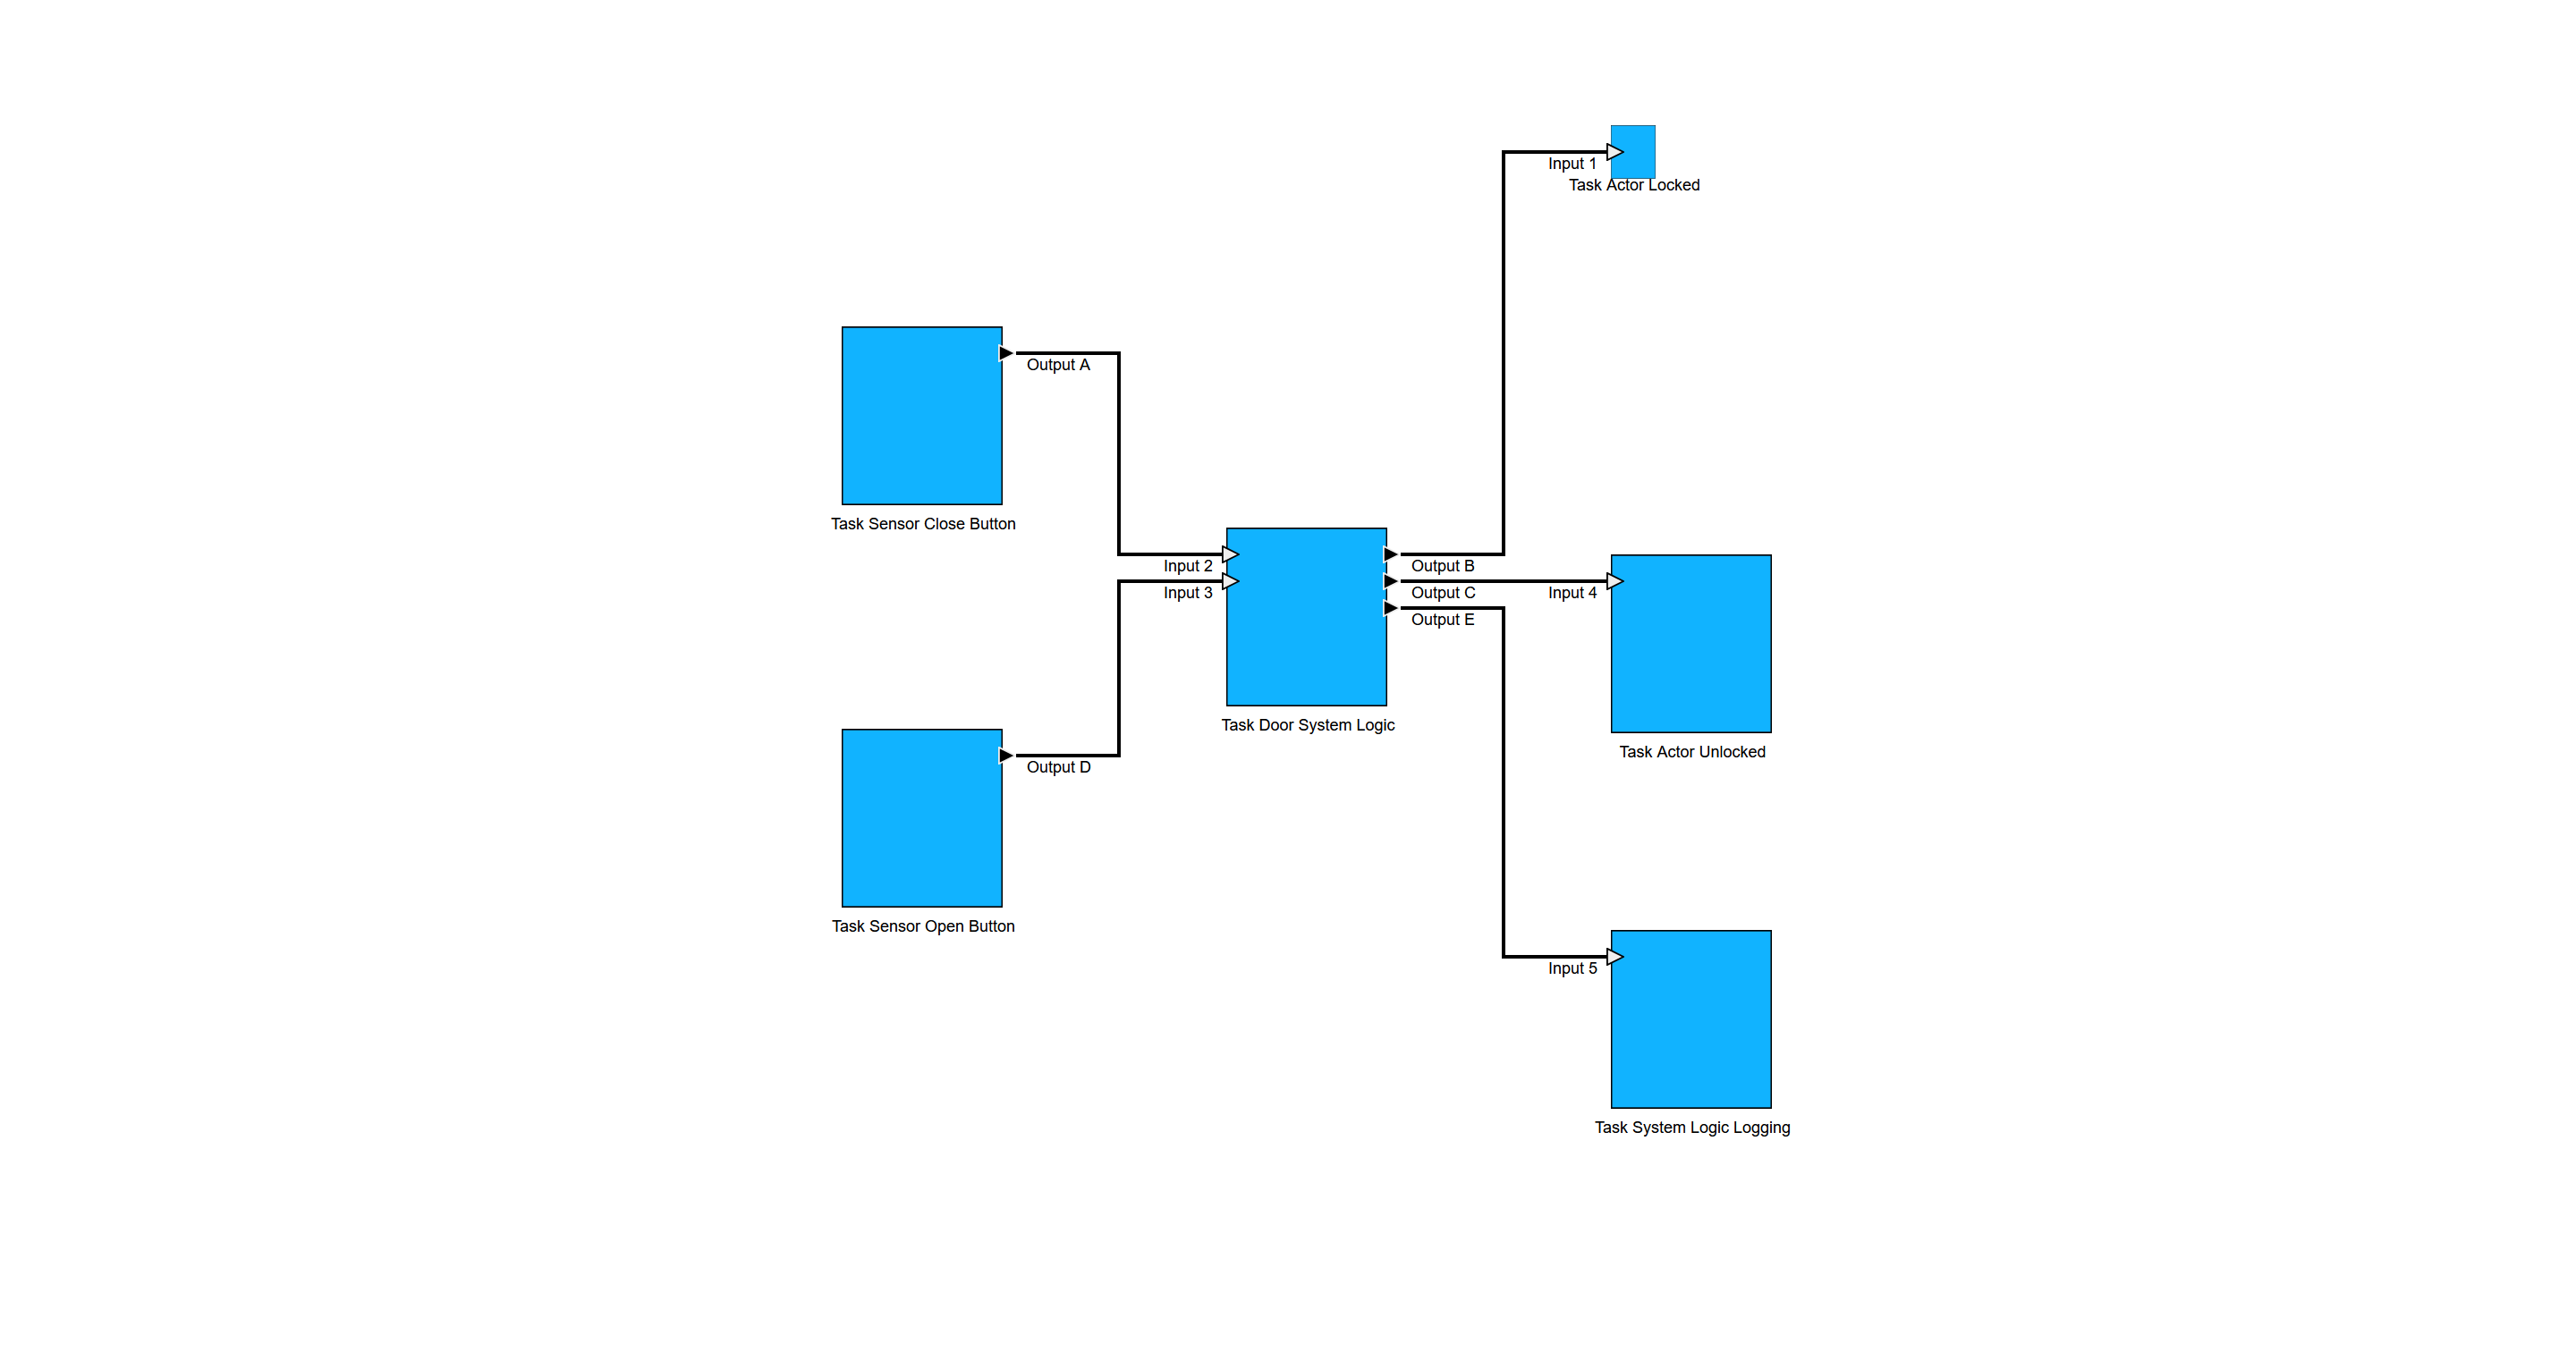
\includegraphics[width=\textwidth]{testcases/vertex_too_small/133525-210774_input_image_after_preprocessing.png}
        \caption*{\textit{Before}}
    \end{subfigure}
    \newline
    \begin{subfigure}[t]{0.9\textwidth}
        \centering
        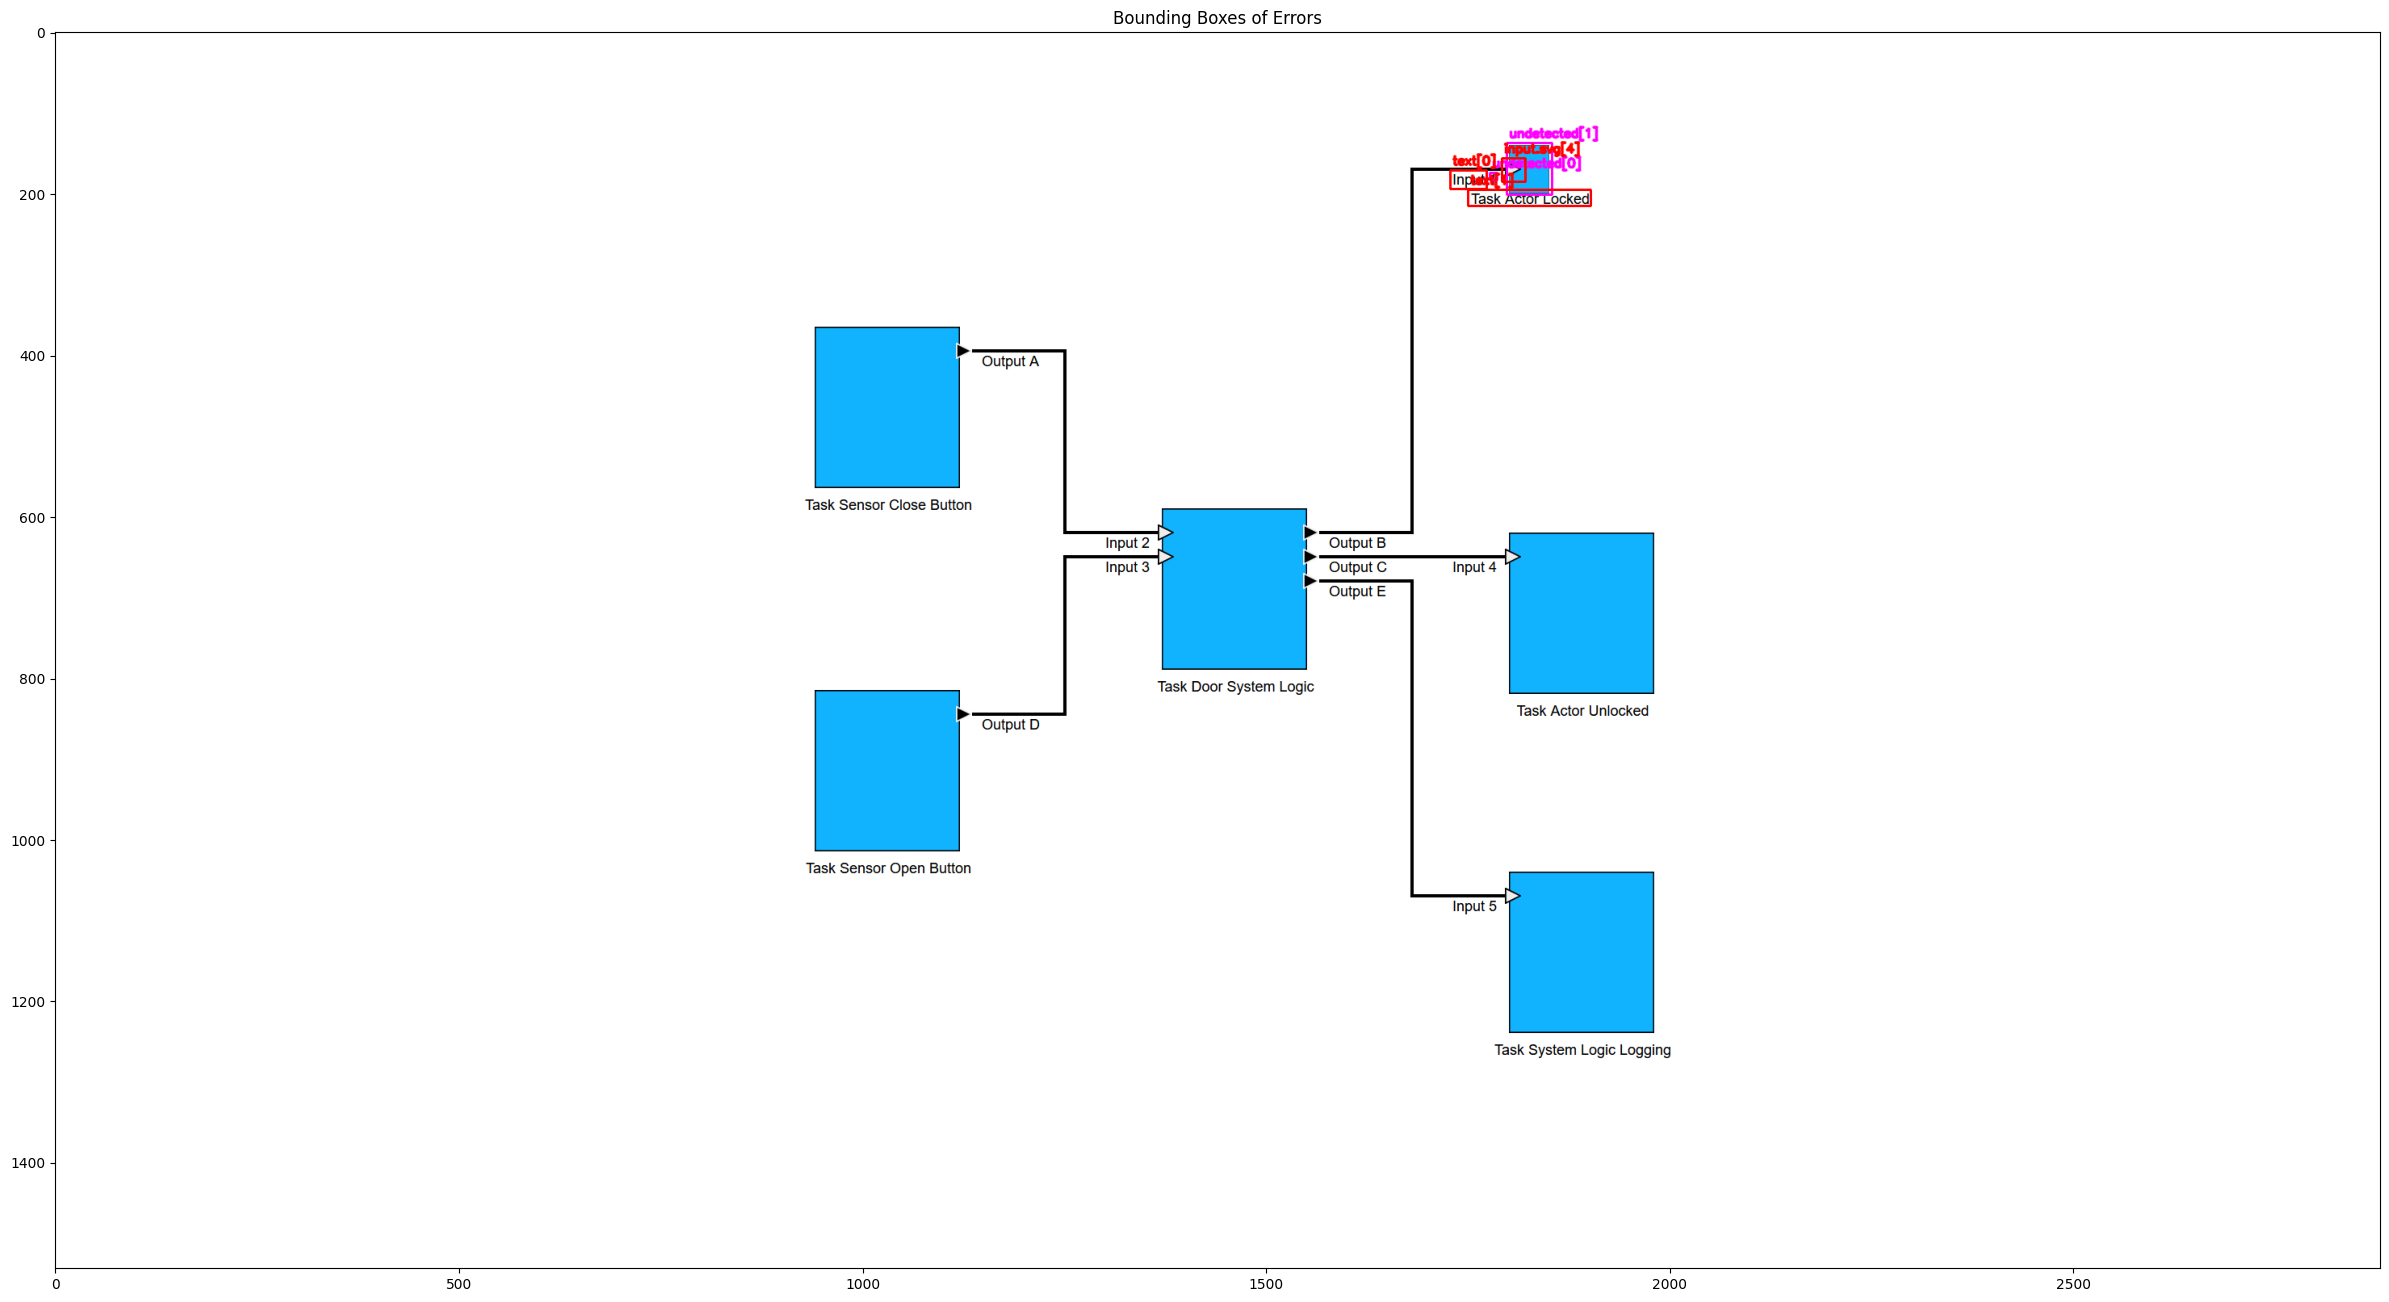
\includegraphics[width=\textwidth]{testcases/vertex_too_small/133600-817717_element_bbox_errors_labeled_colored.png}
        \caption*{\textit{After}}
    \end{subfigure}
    % \caption{Vertex too small}
    \label{fig:vertex_too_small}
\end{figure}
\newpage

\section{Vertex too large}
\begin{figure}[H]
    \centering
    \begin{subfigure}[t]{0.9\textwidth}
        \centering
        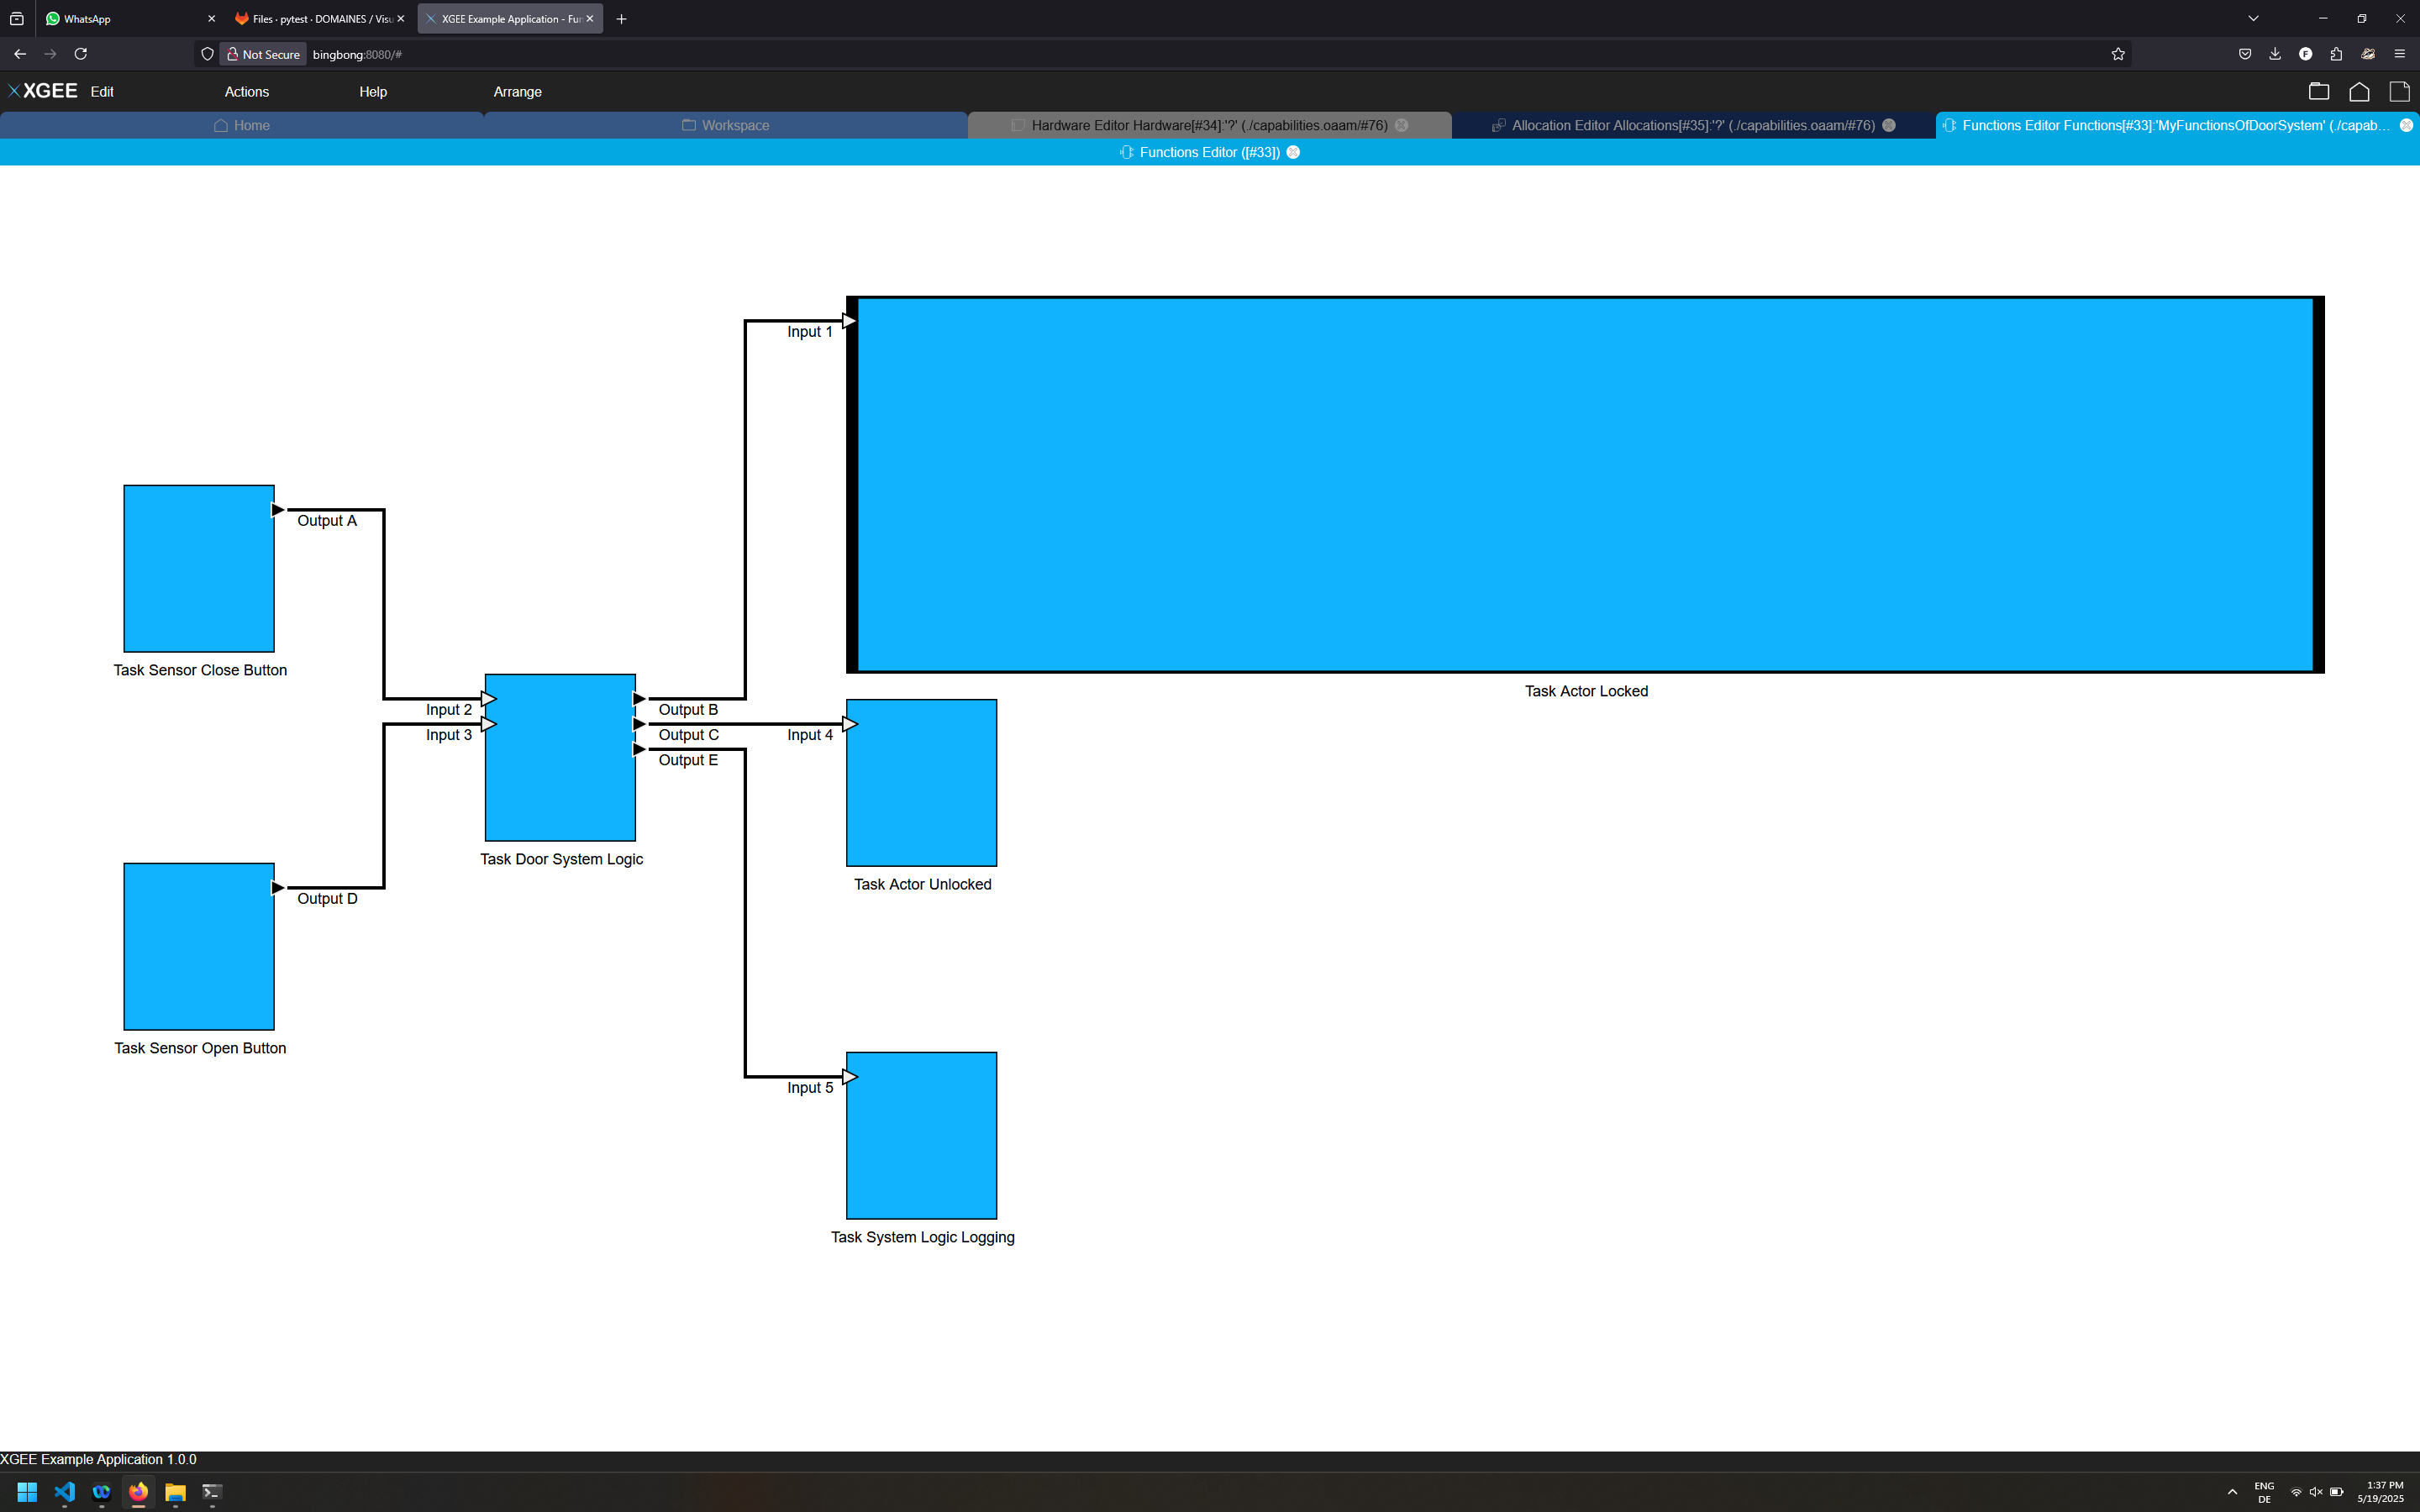
\includegraphics[width=\textwidth]{testcases/vertex_too_large/133708-898563_input_image.png}
        \caption*{\textit{Before}}
    \end{subfigure}
    \newline
    \begin{subfigure}[t]{0.9\textwidth}
        \centering
        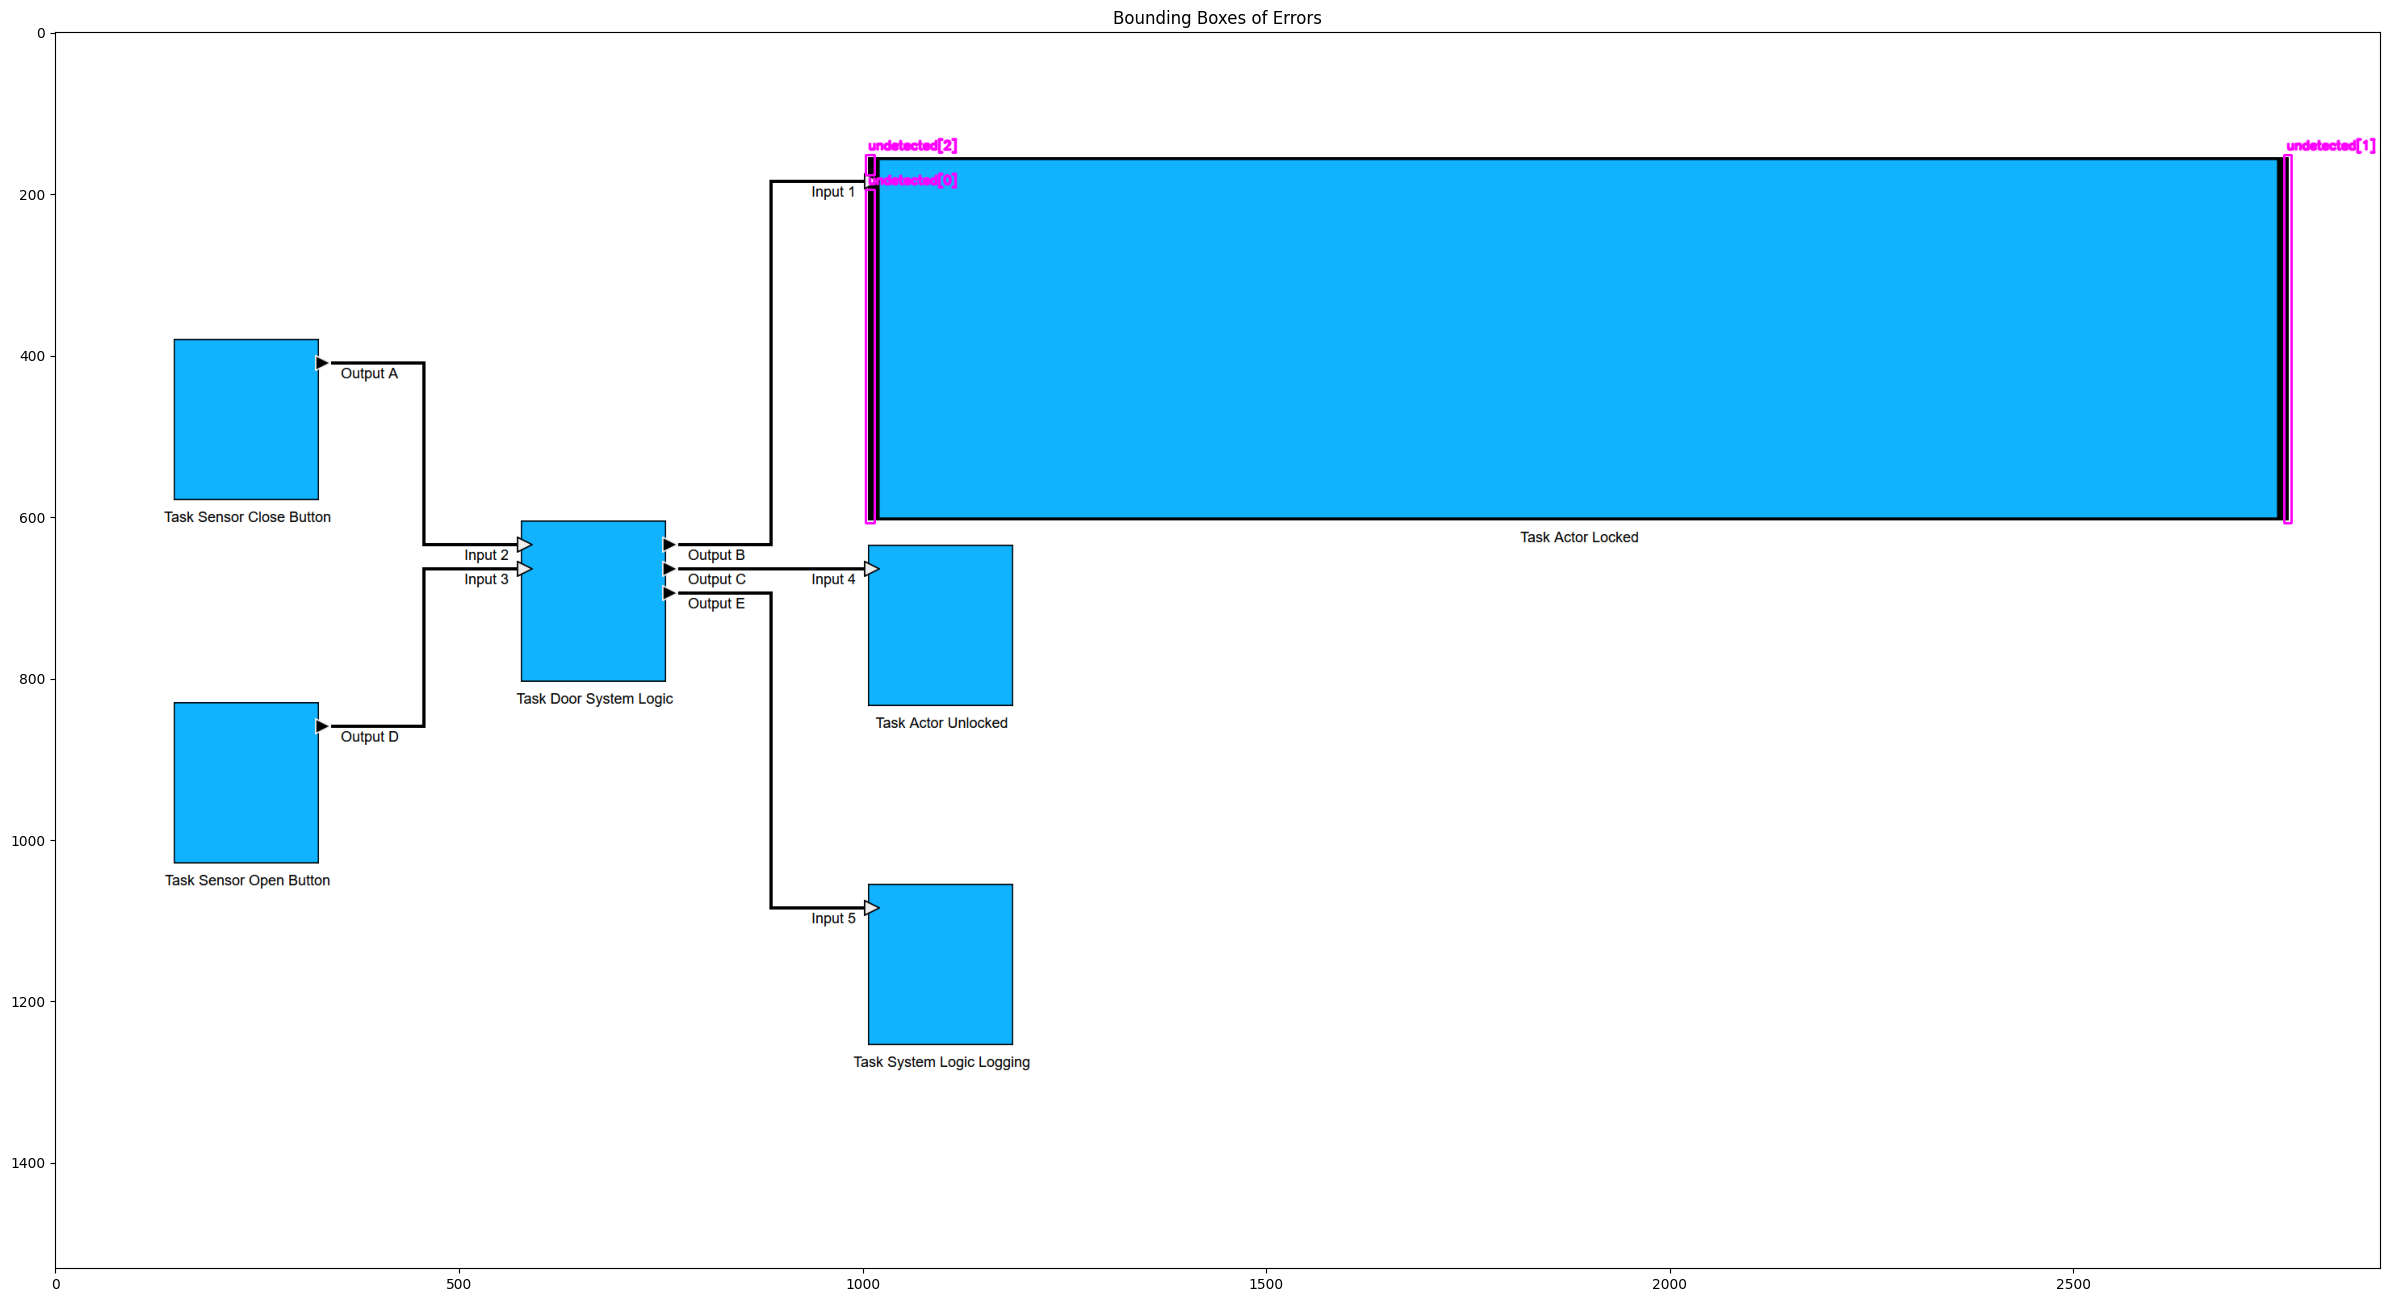
\includegraphics[width=\textwidth]{testcases/vertex_too_large/133744-868019_element_bbox_errors_labeled_colored.png}
        \caption*{\textit{After}}
    \end{subfigure}
    % \caption{Vertex too large}
    \label{fig:vertex_too_large}
\end{figure}
\newpage

\section{Vertex wrong color}
\begin{figure}[H]
    \centering
    \begin{subfigure}[t]{0.9\textwidth}
        \centering
        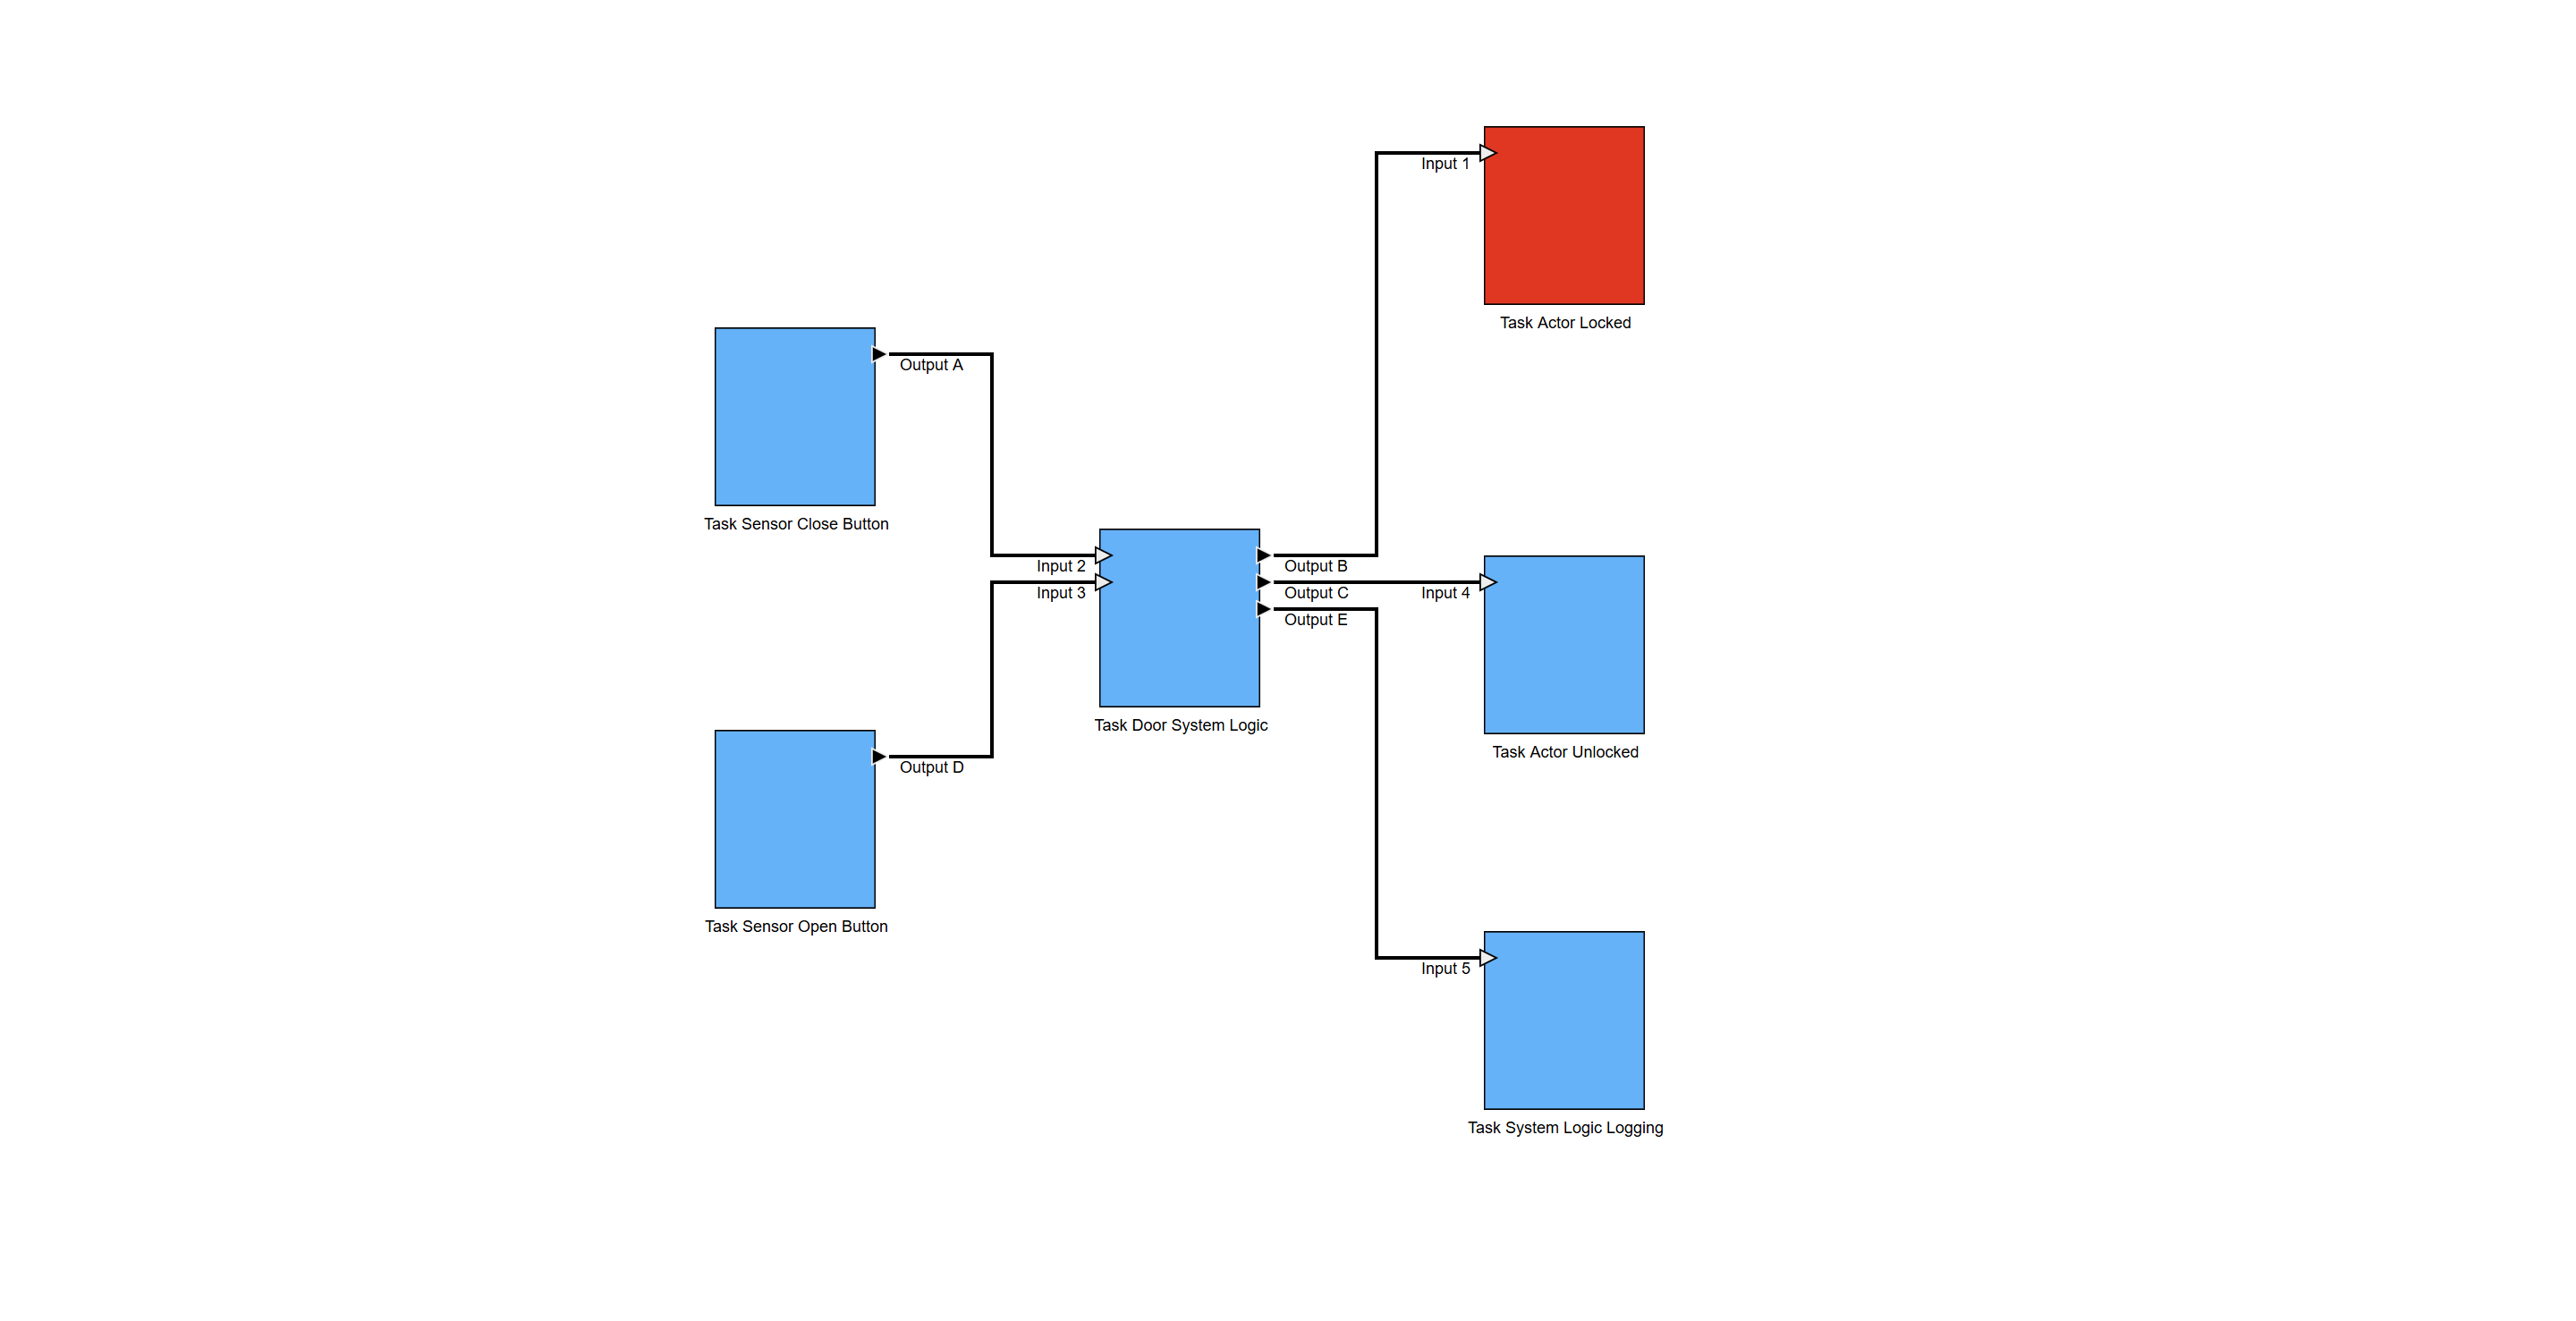
\includegraphics[width=\textwidth]{testcases/vertex_wrong_color/134341-480129_input_image_after_preprocessing.png}
        \caption*{\textit{Before}}
    \end{subfigure}
    \newline    
    \begin{subfigure}[t]{0.9\textwidth}
        \centering
        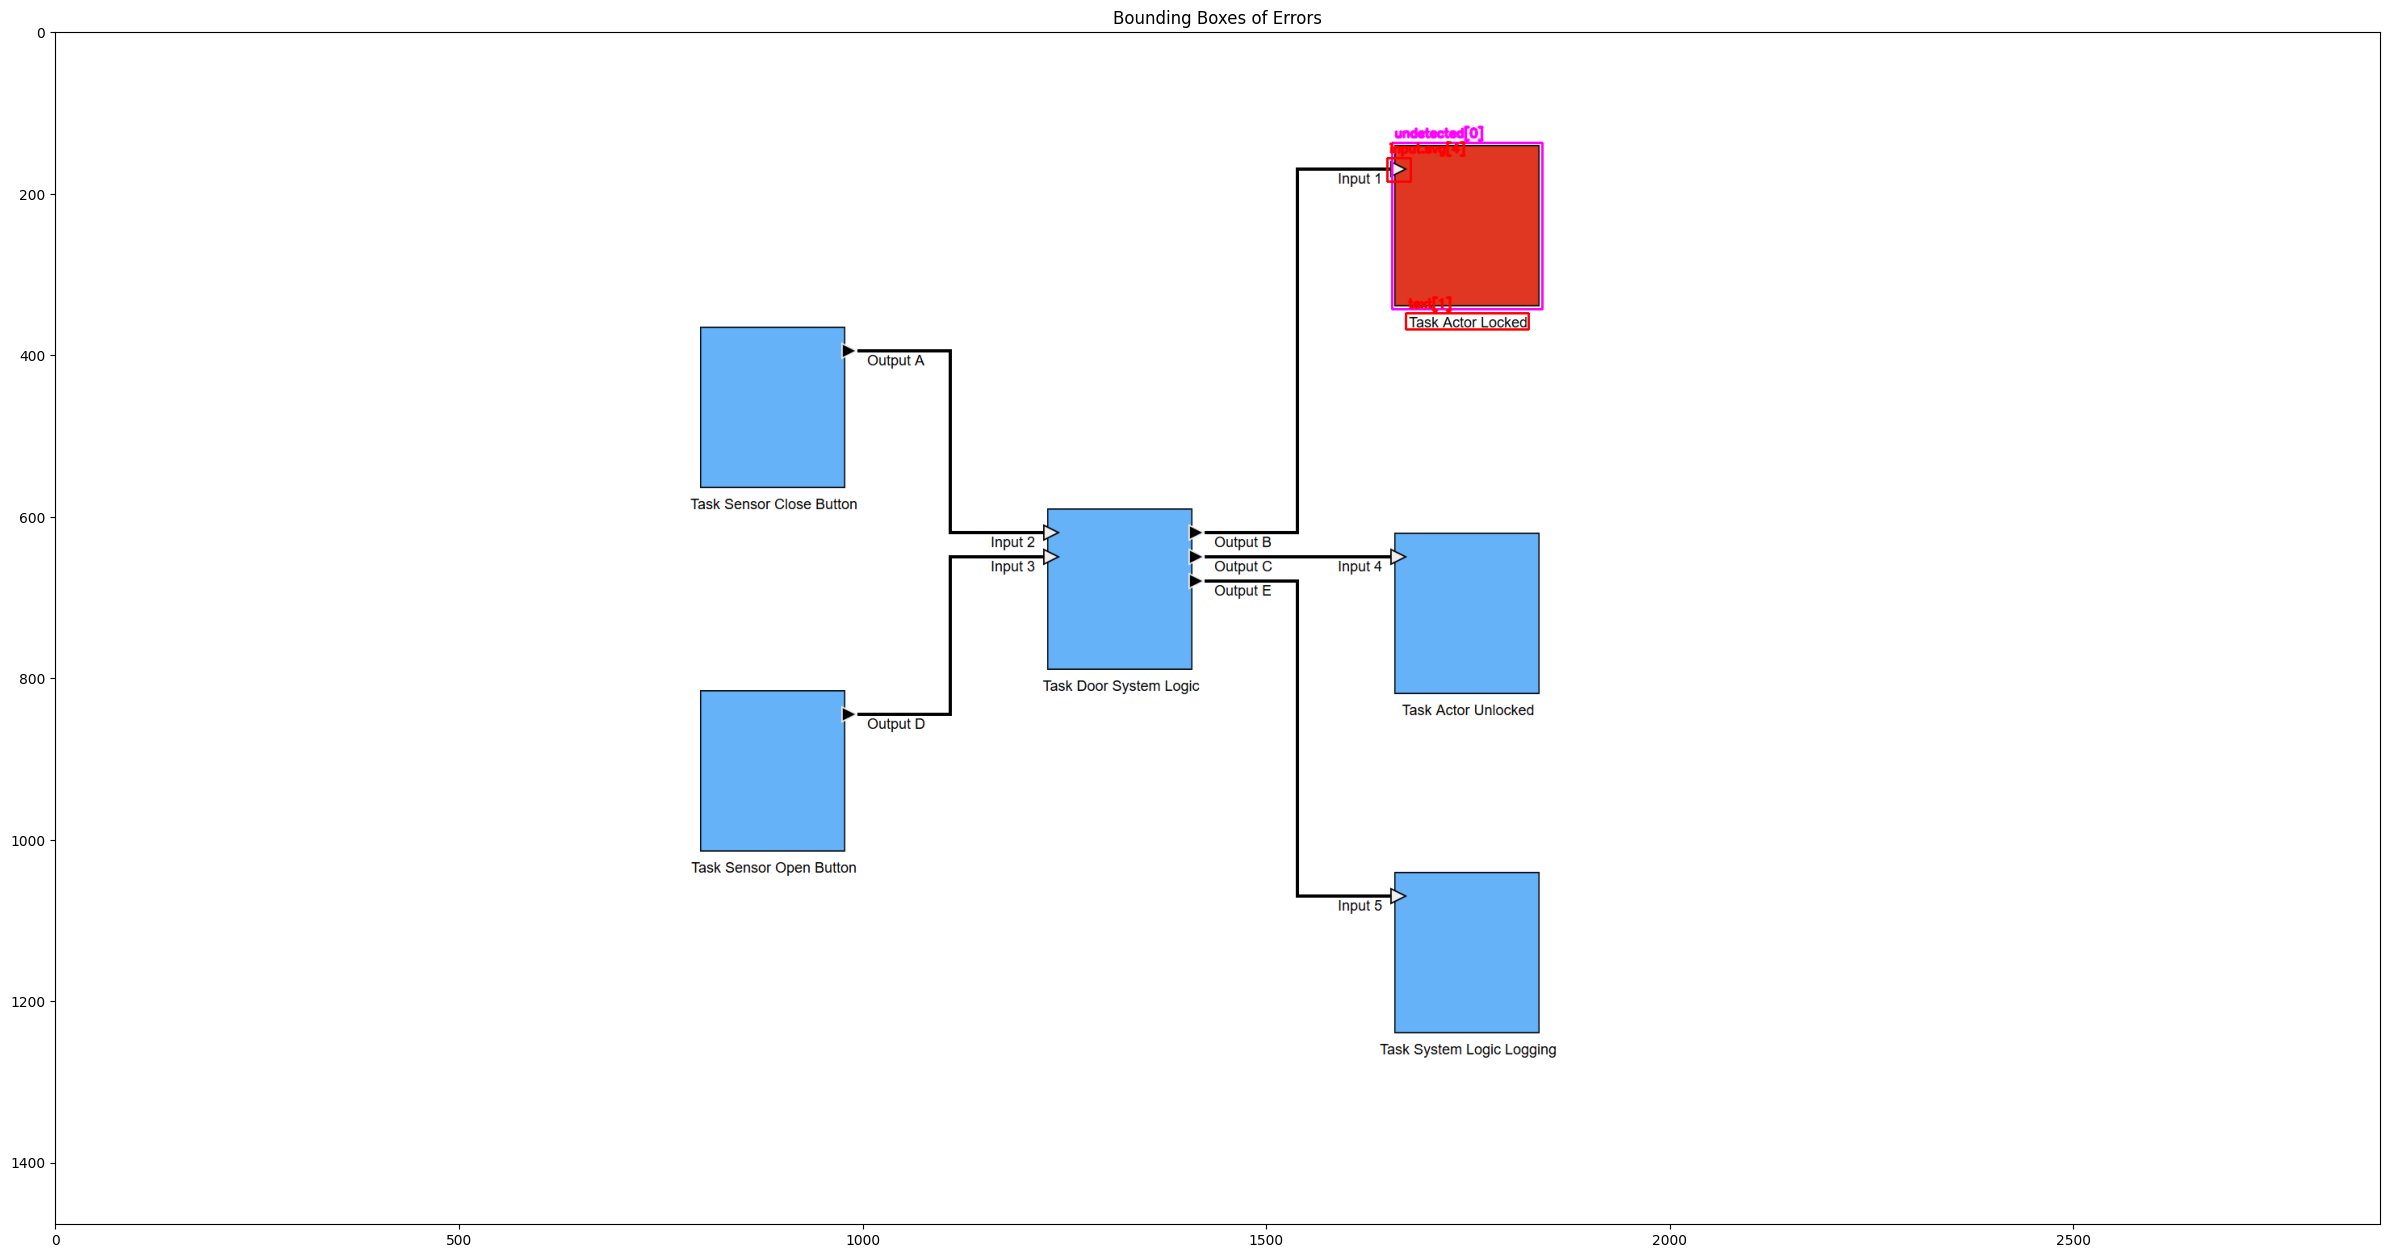
\includegraphics[width=\textwidth]{testcases/vertex_wrong_color/134401-825366_element_bbox_errors_labeled_colored.png}
        \caption*{\textit{After}}
    \end{subfigure}
    % \caption{Vertex wrong color}
    \label{fig:vertex_wrong_color}
\end{figure}
\newpage

\section{Vertex in wrong position}
\begin{figure}[H]
    \centering
    \begin{subfigure}[t]{0.9\textwidth}
        \centering
        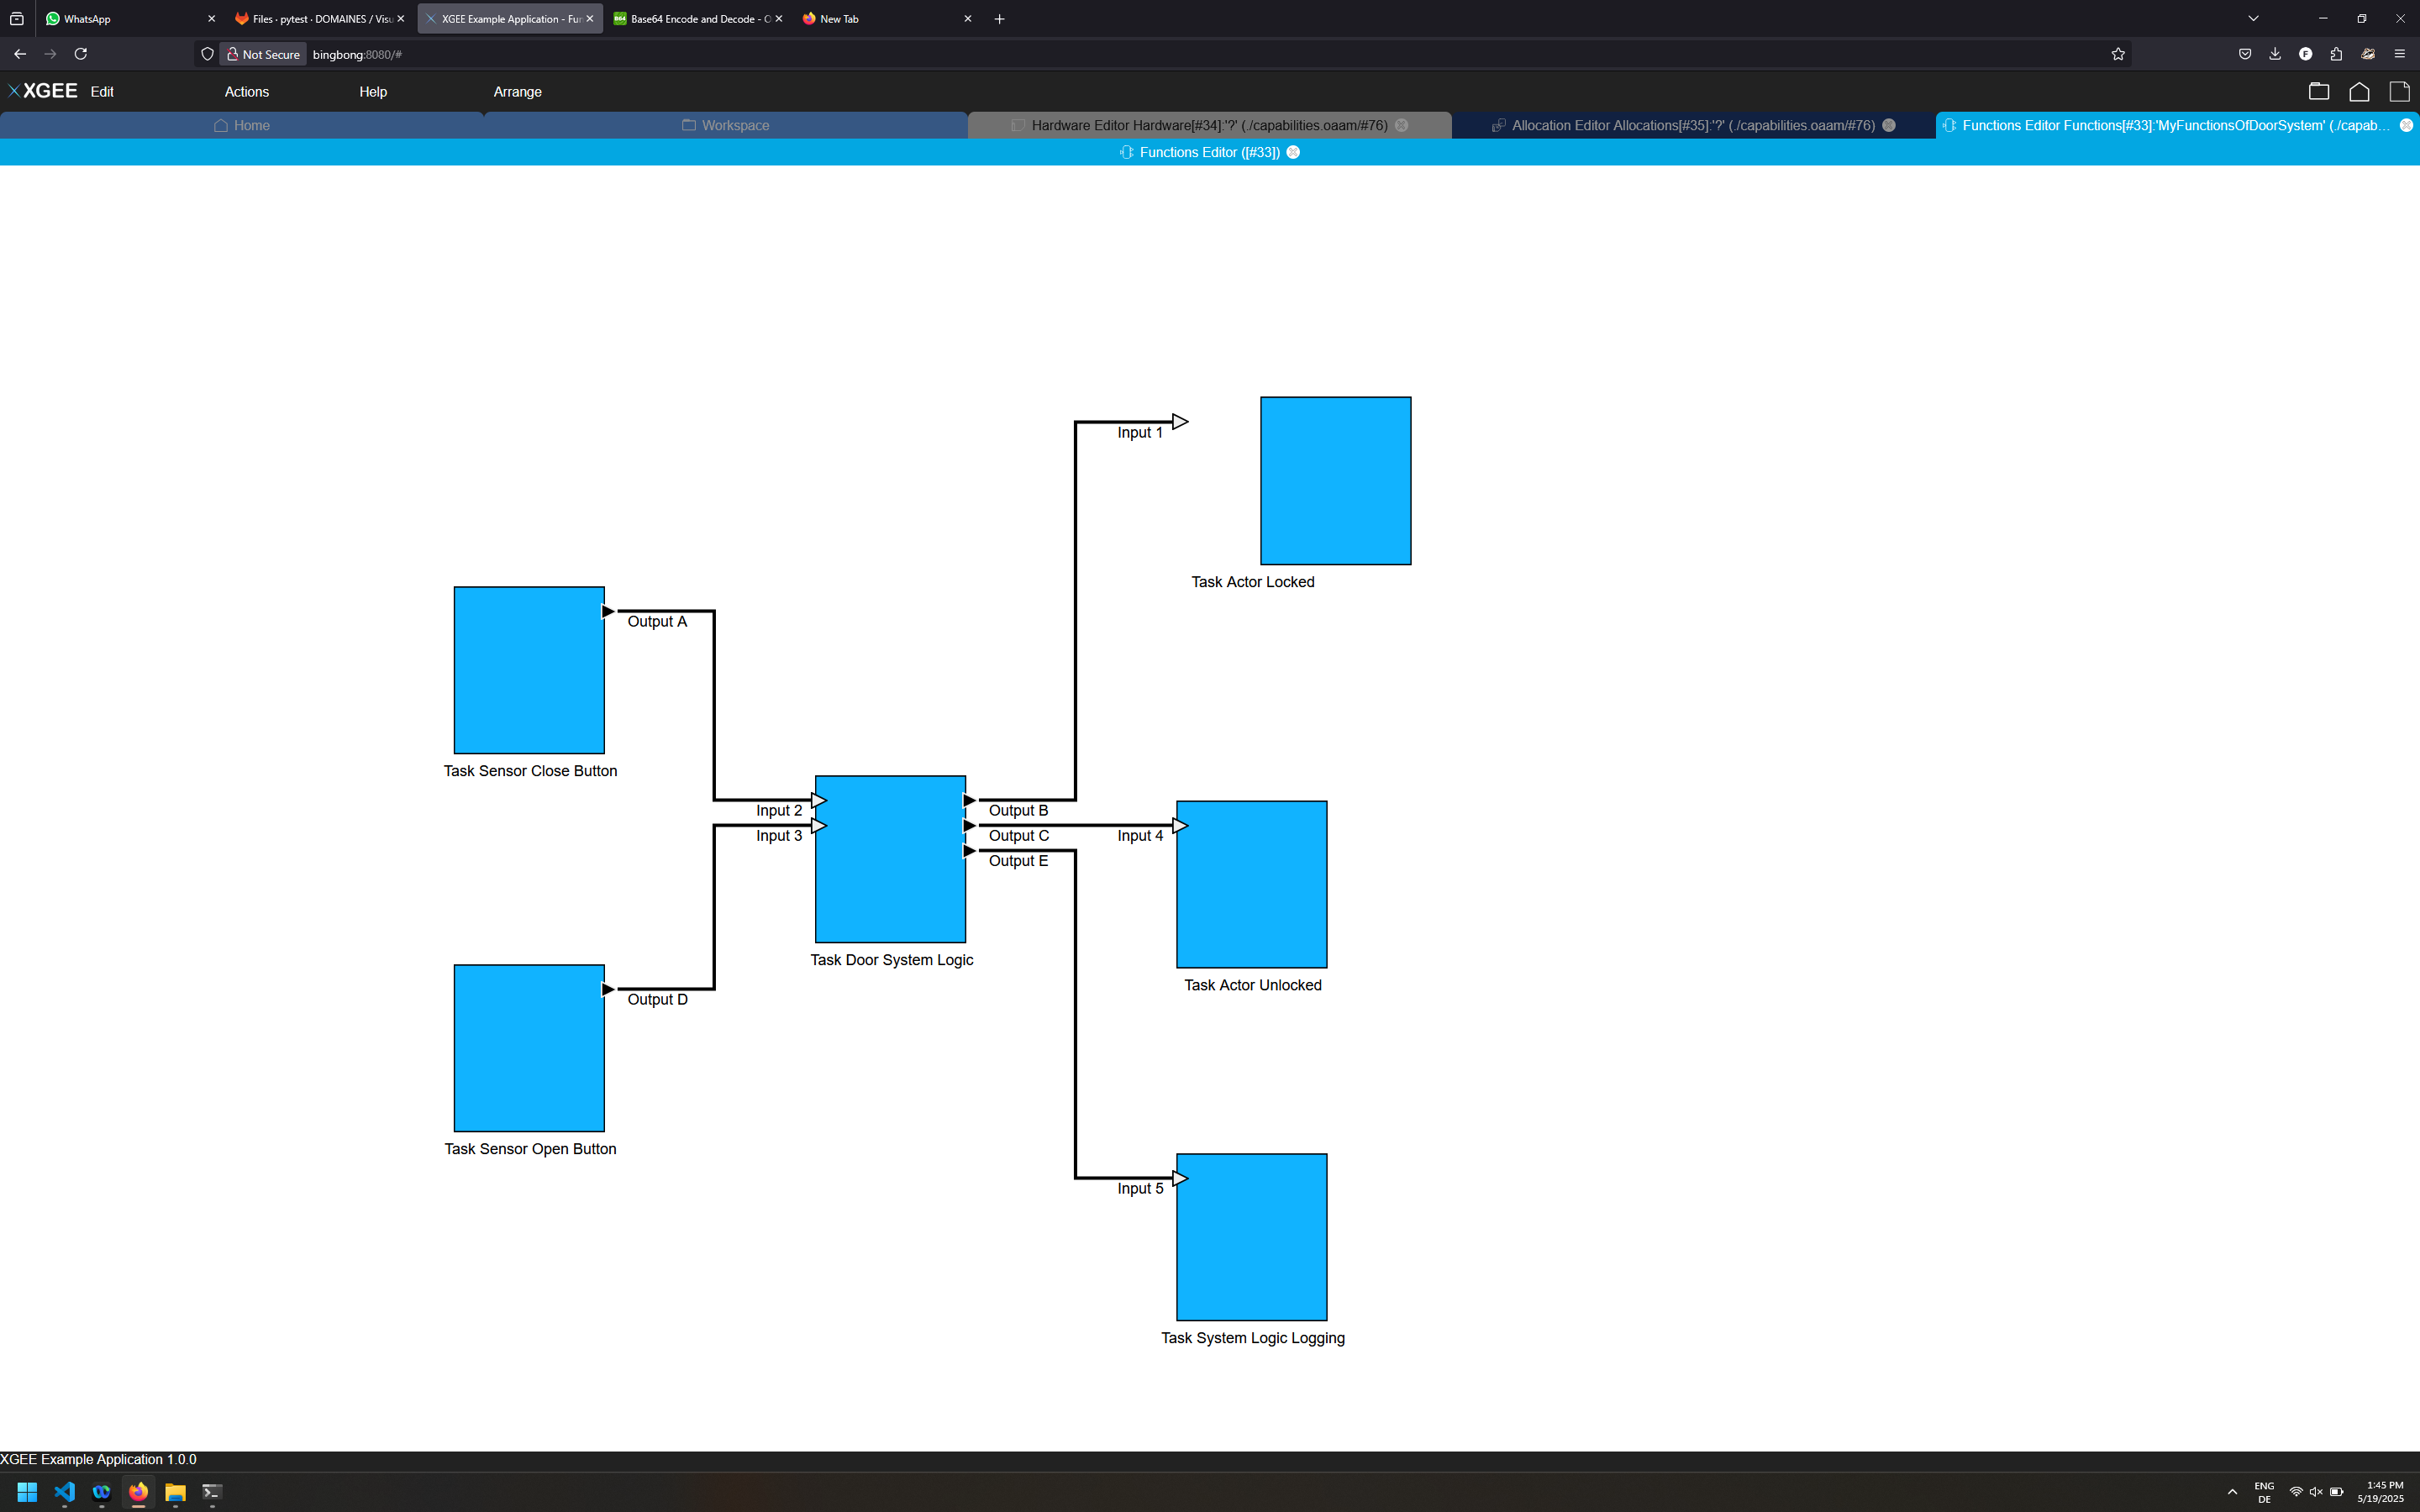
\includegraphics[width=\textwidth]{testcases/vertex_task_wrong_position/134530-573593_input_image.png}
        \caption*{\textit{Before}}
    \end{subfigure}
    \newline
    \begin{subfigure}[t]{0.9\textwidth}
        \centering
        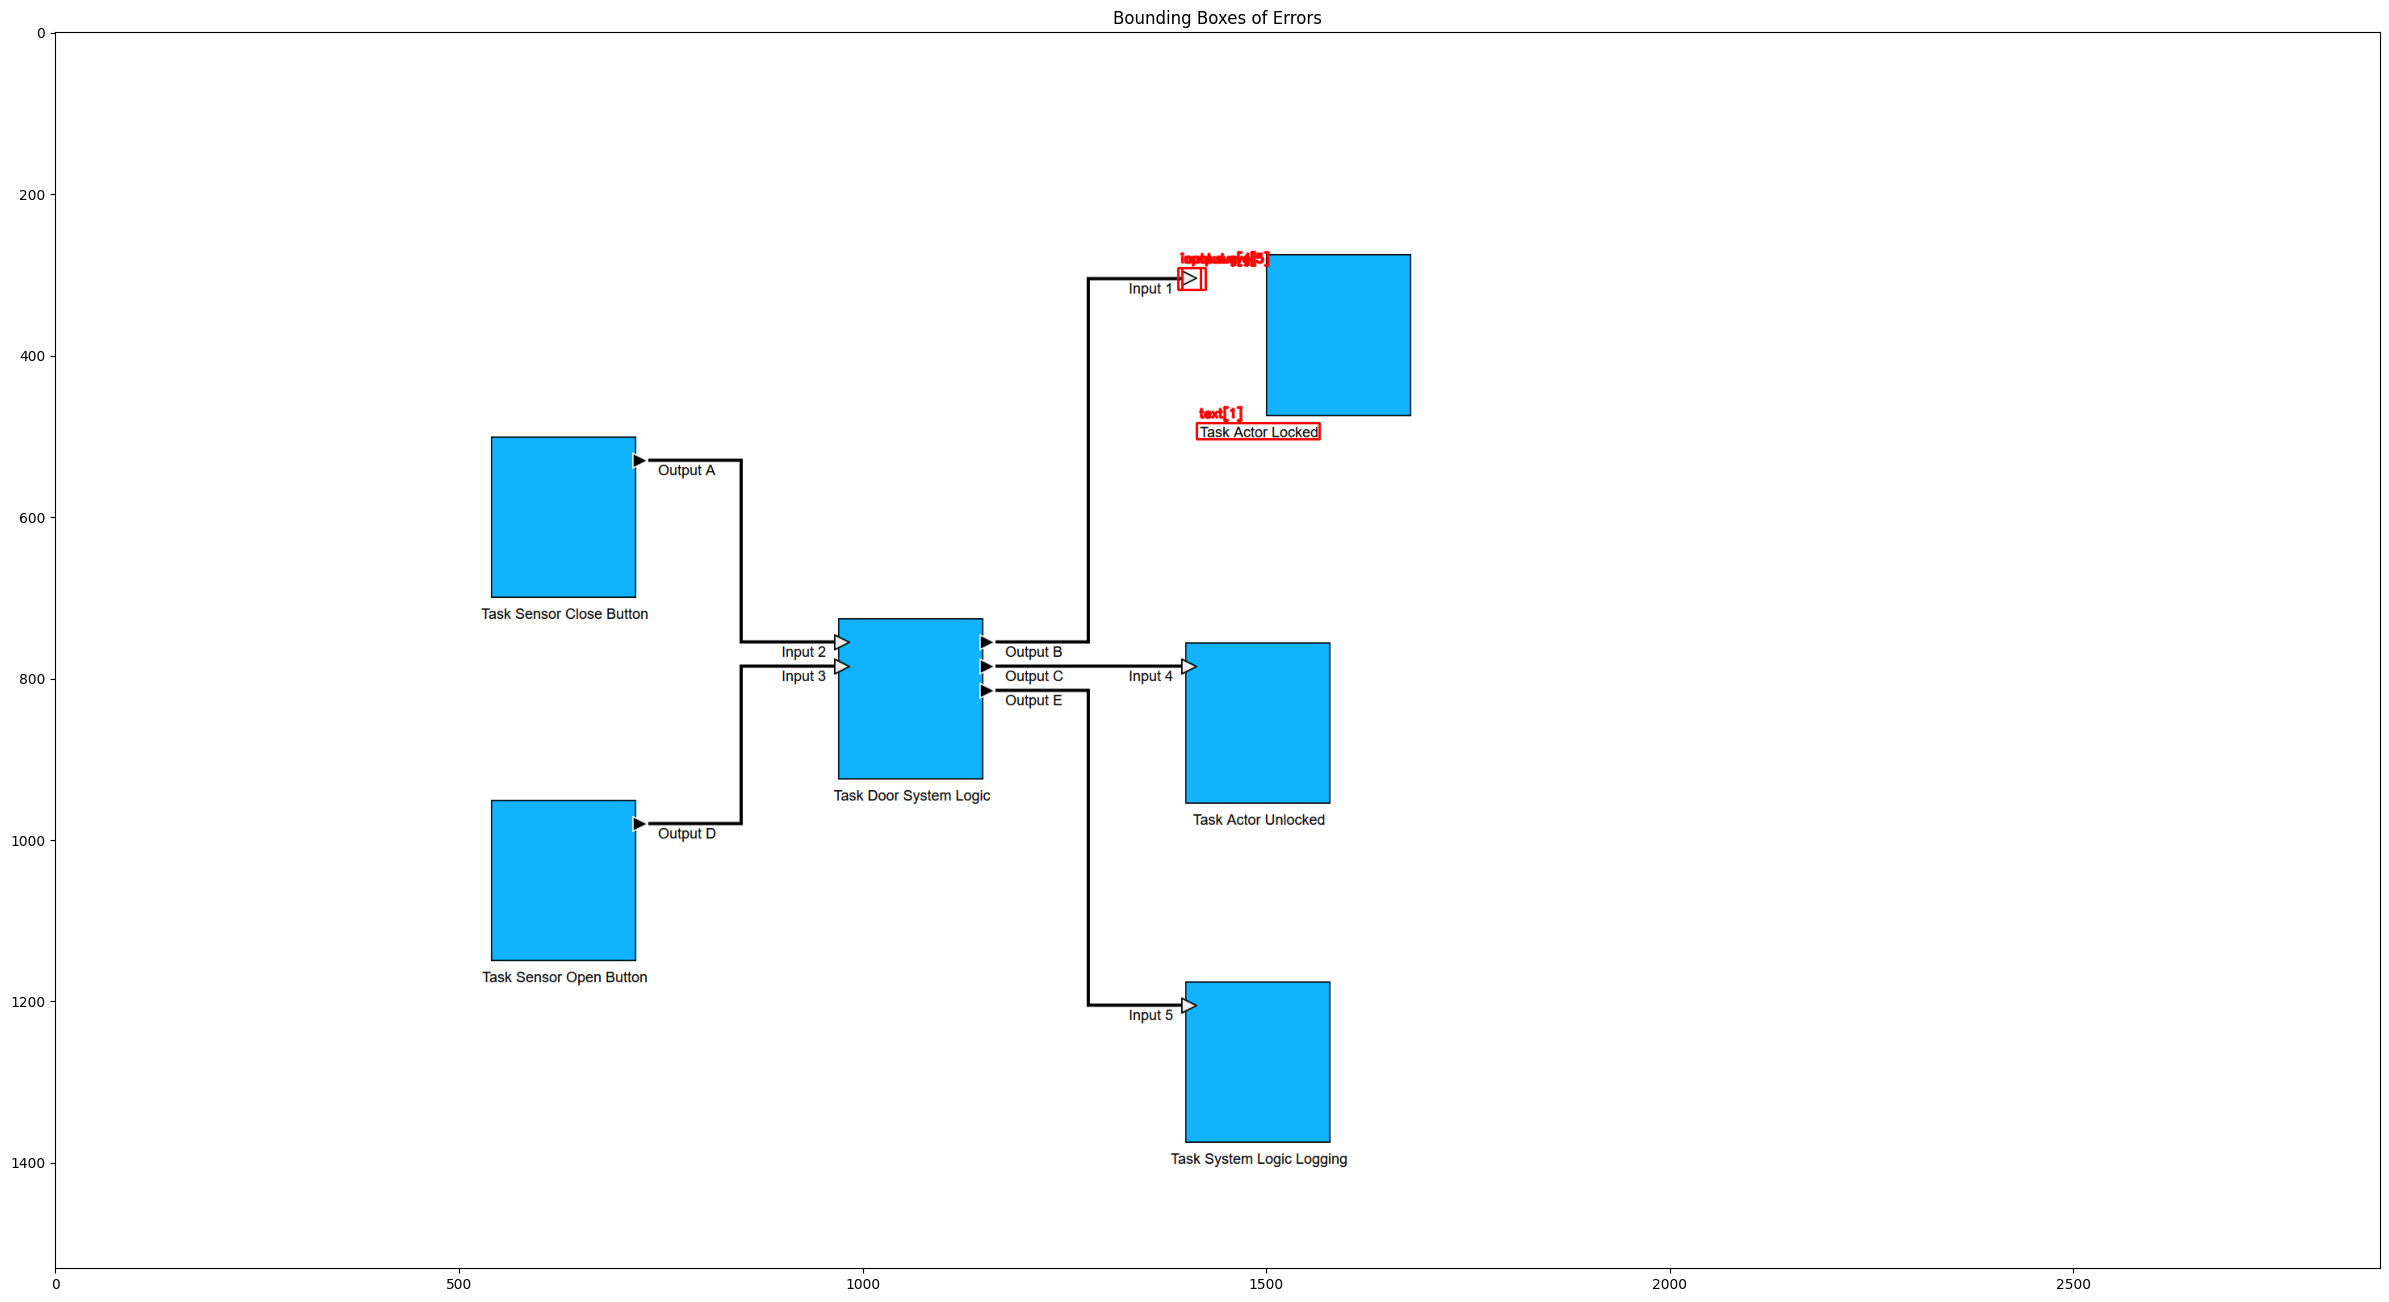
\includegraphics[width=\textwidth]{testcases/vertex_task_wrong_position/134550-162424_element_bbox_errors_labeled_colored.png}
        \caption*{\textit{After}}
    \end{subfigure}
    % \caption{Vertex in wrong position}
    \label{fig:vertex_wrong_position}
\end{figure}
\newpage

\section{Vertex input in wrong position}
\begin{figure}[H]
    \centering
    \begin{subfigure}[t]{0.9\textwidth}
        \centering
        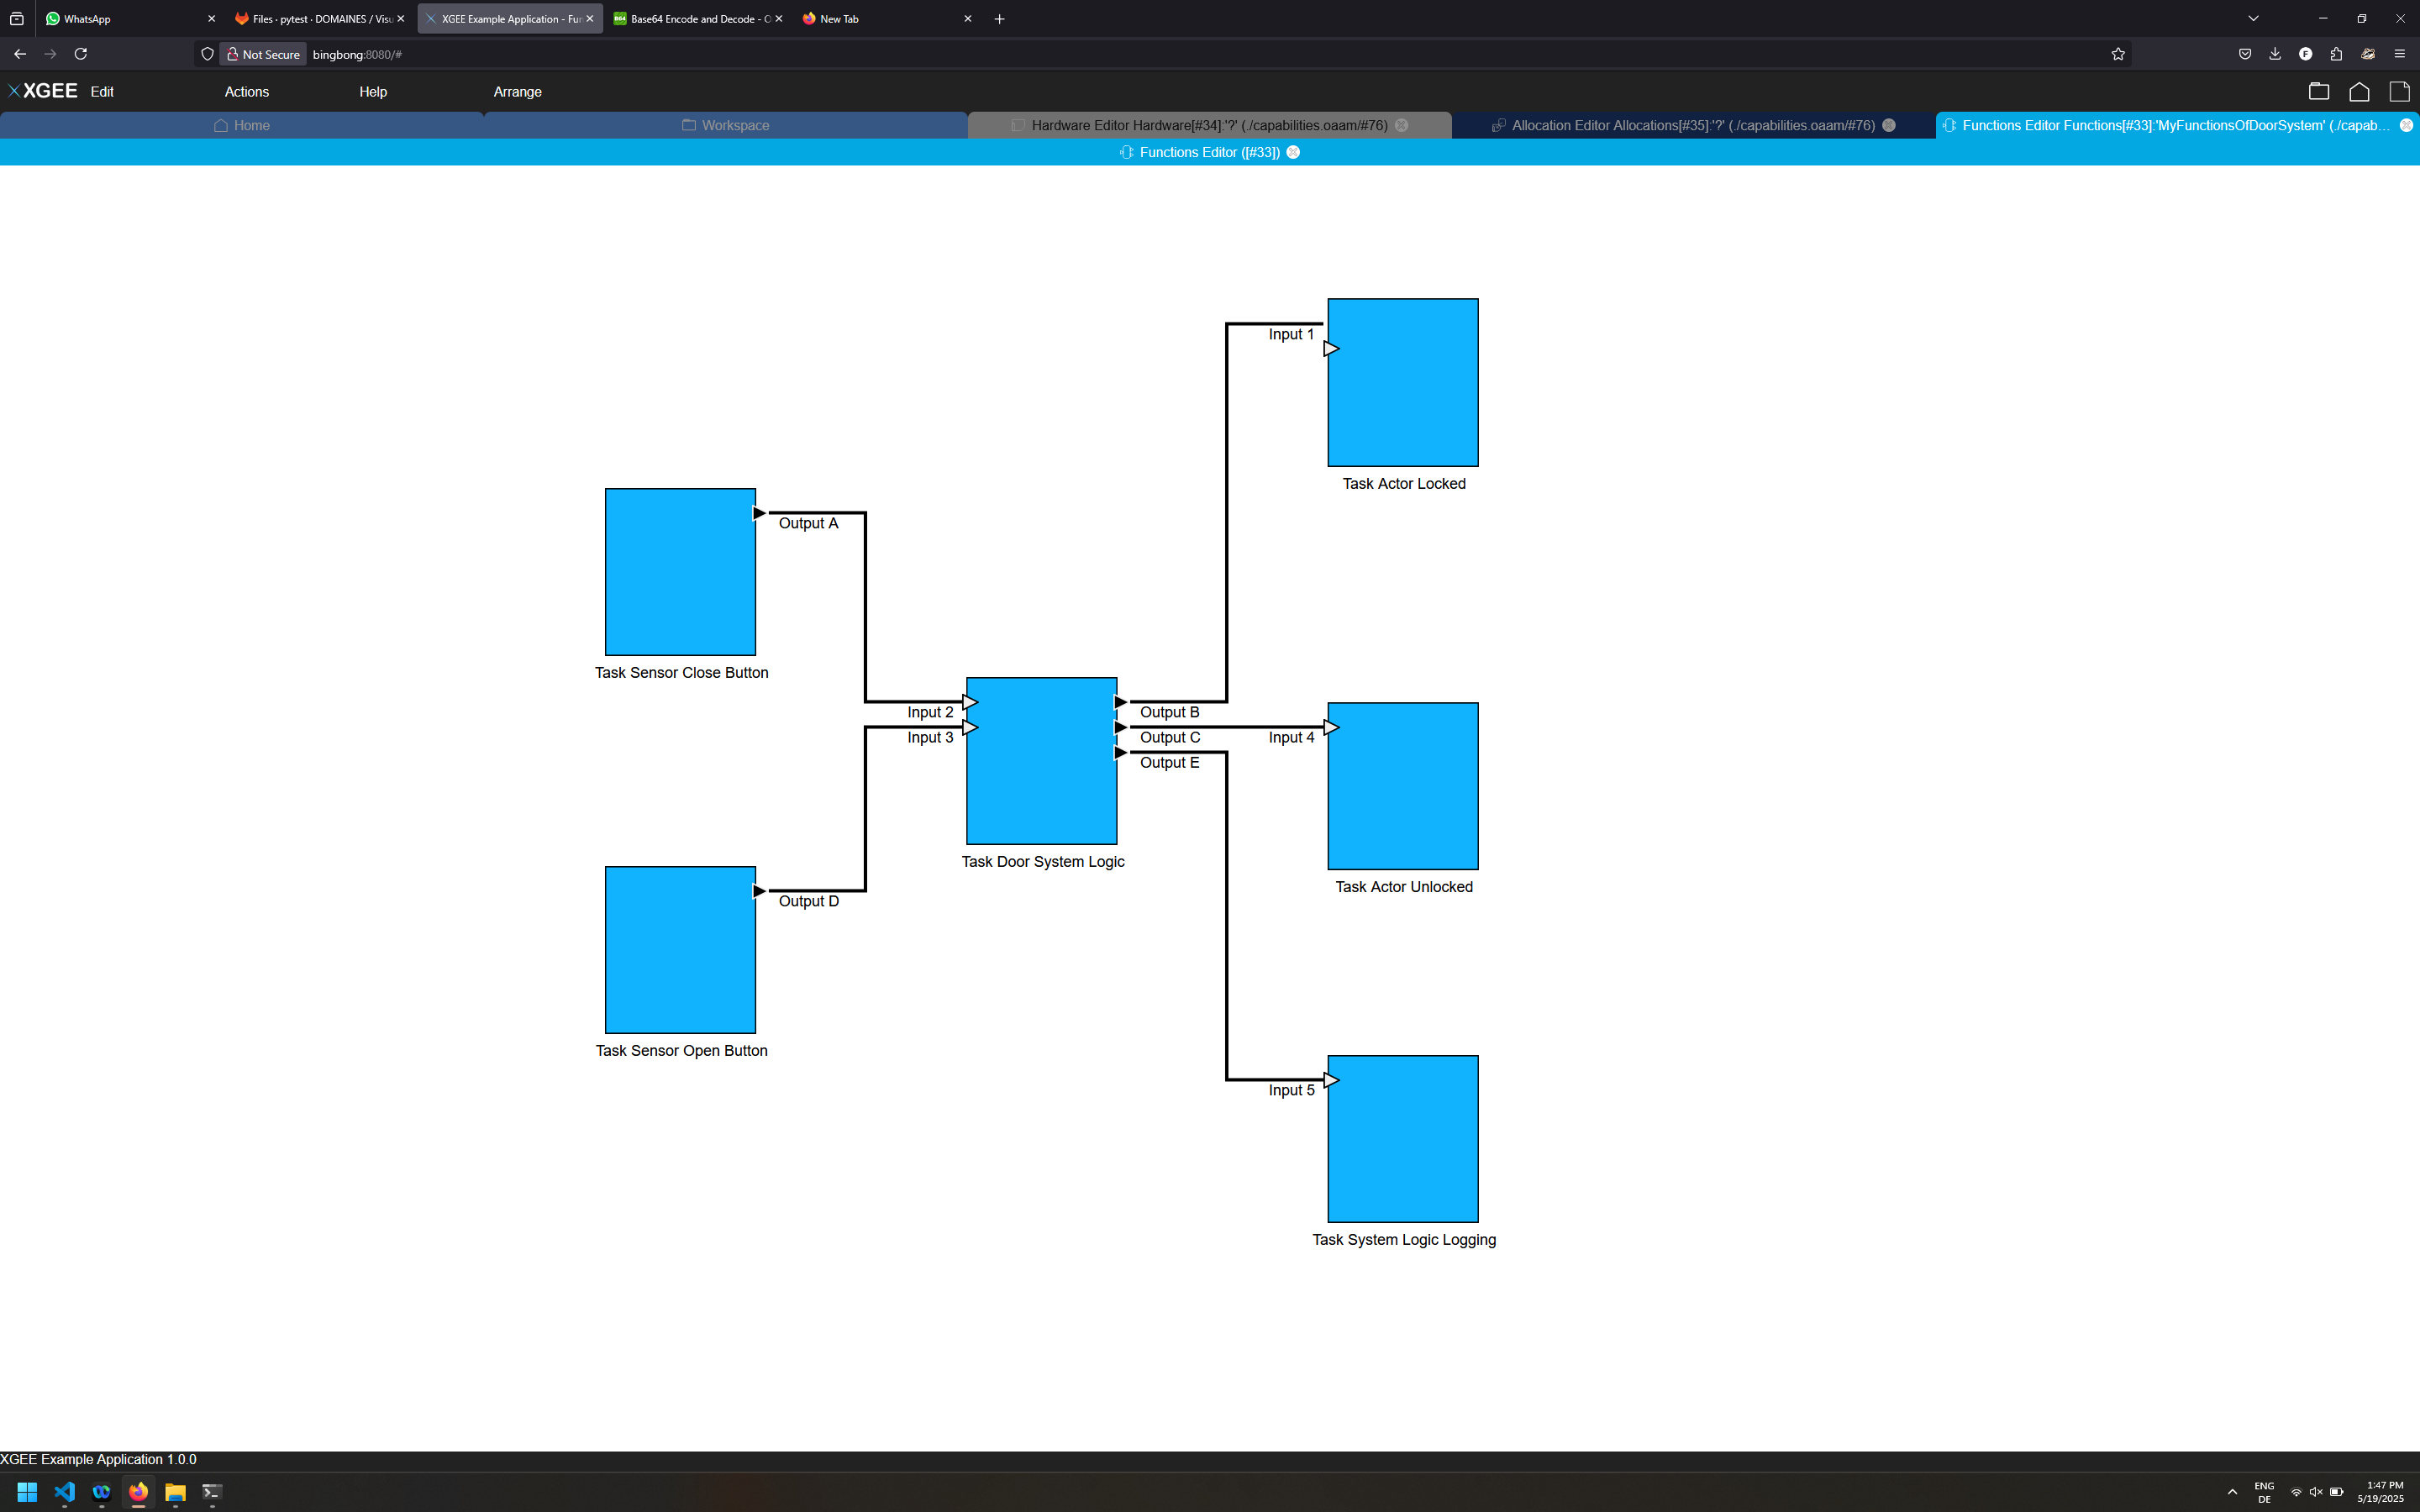
\includegraphics[width=\textwidth]{testcases/vertex_input_wrong_position/134736-128123_input_image.png}
        \caption*{\textit{Before}}
    \end{subfigure}
    \newline
    \begin{subfigure}[t]{0.9\textwidth}
        \centering
        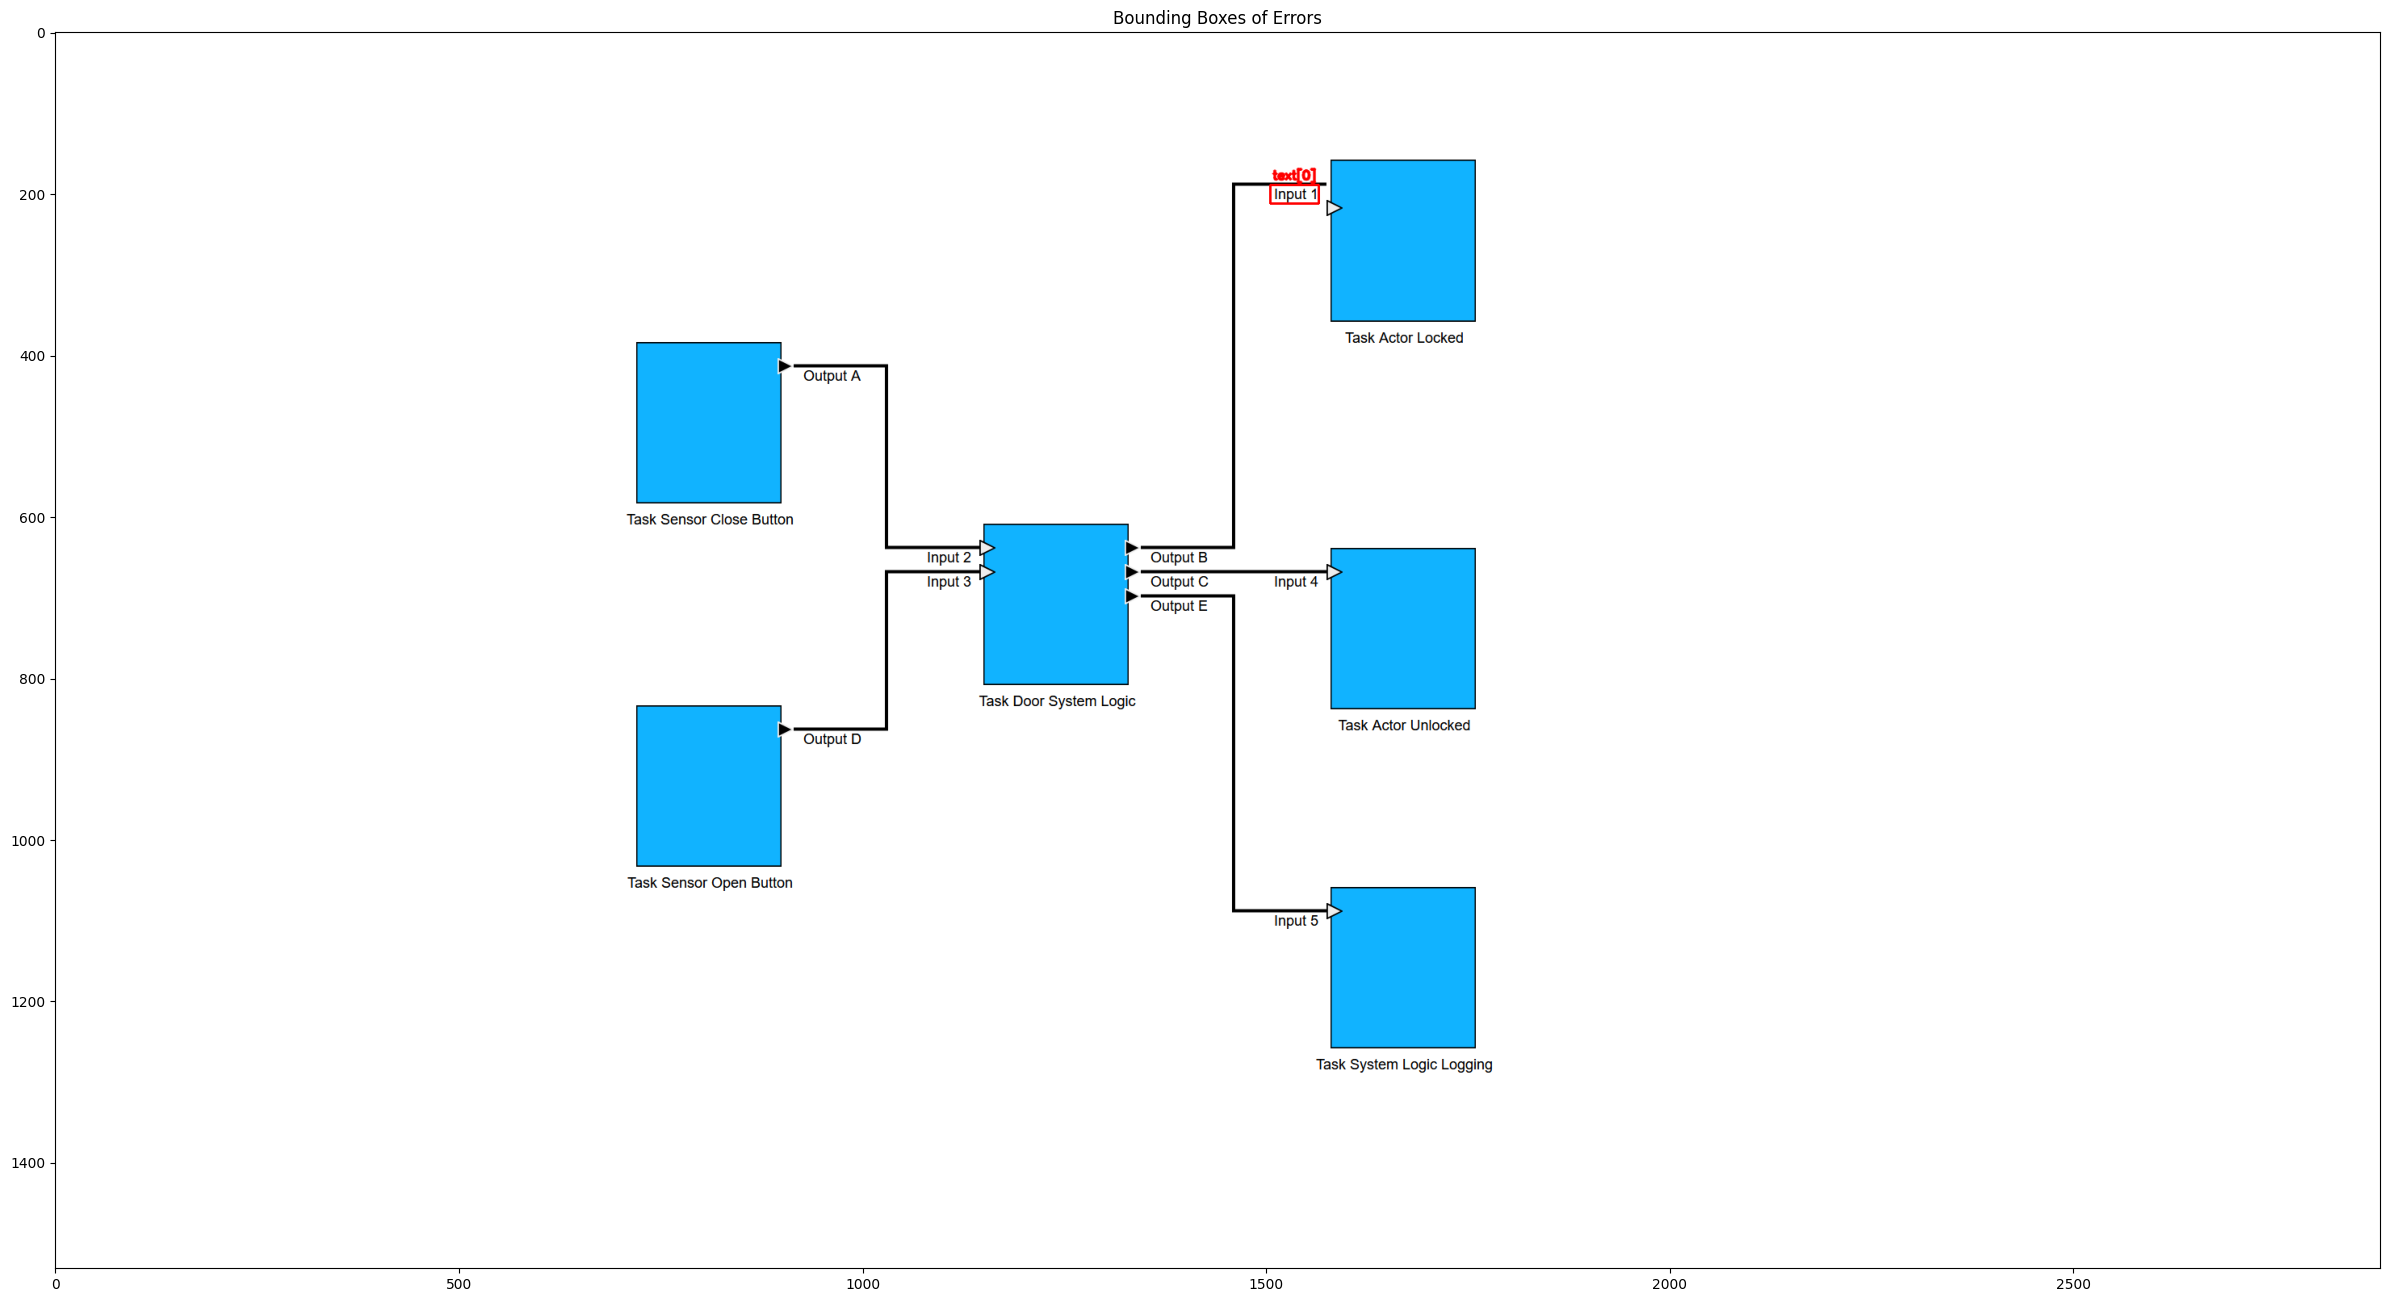
\includegraphics[width=\textwidth]{testcases/vertex_input_wrong_position/134756-619713_element_bbox_errors_labeled_colored.png}
        \caption*{\textit{After}}
    \end{subfigure}
    % \caption{Vertex in model, but not in visualization}
    \label{fig:vertex_input_wrong_position}
\end{figure}
\newpage

\section{Vertex task in wrong position}
\begin{figure}[H]
    \centering
    \begin{subfigure}[t]{0.9\textwidth}
        \centering
        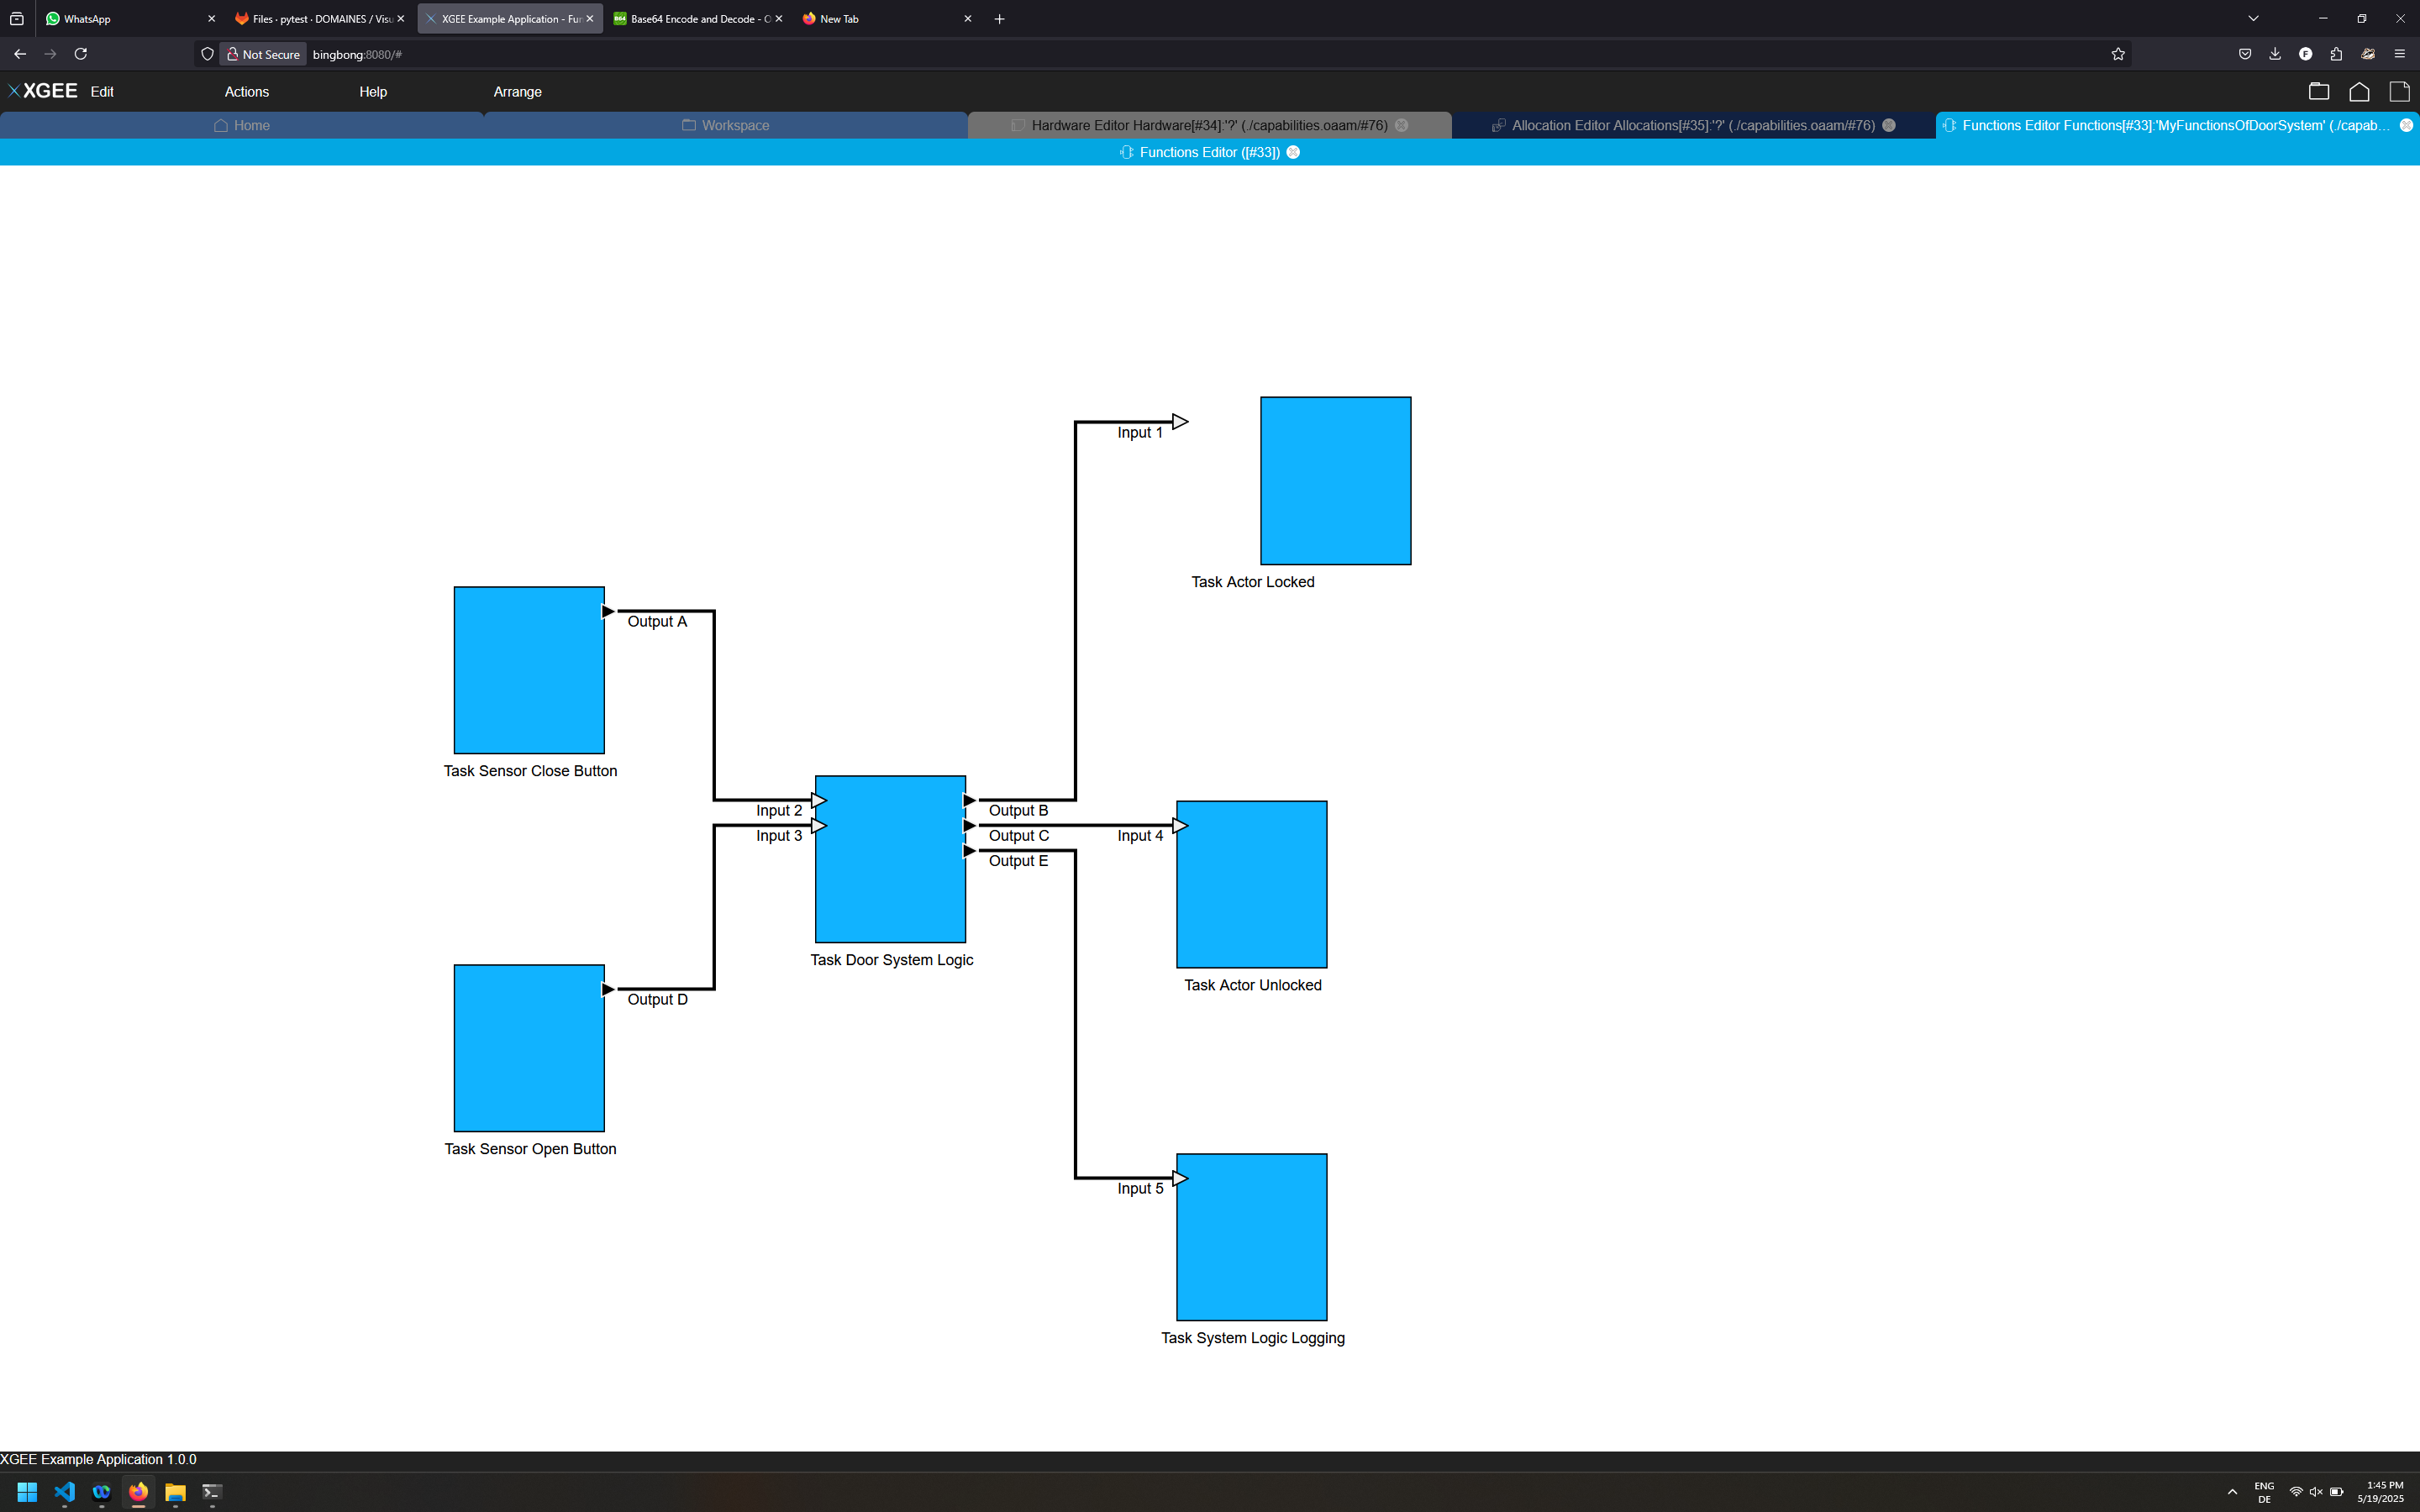
\includegraphics[width=\textwidth]{testcases/vertex_task_wrong_position/134530-573593_input_image.png}
        \caption*{\textit{Before}}
    \end{subfigure}
    \newline
    \begin{subfigure}[t]{0.9\textwidth}
        \centering
        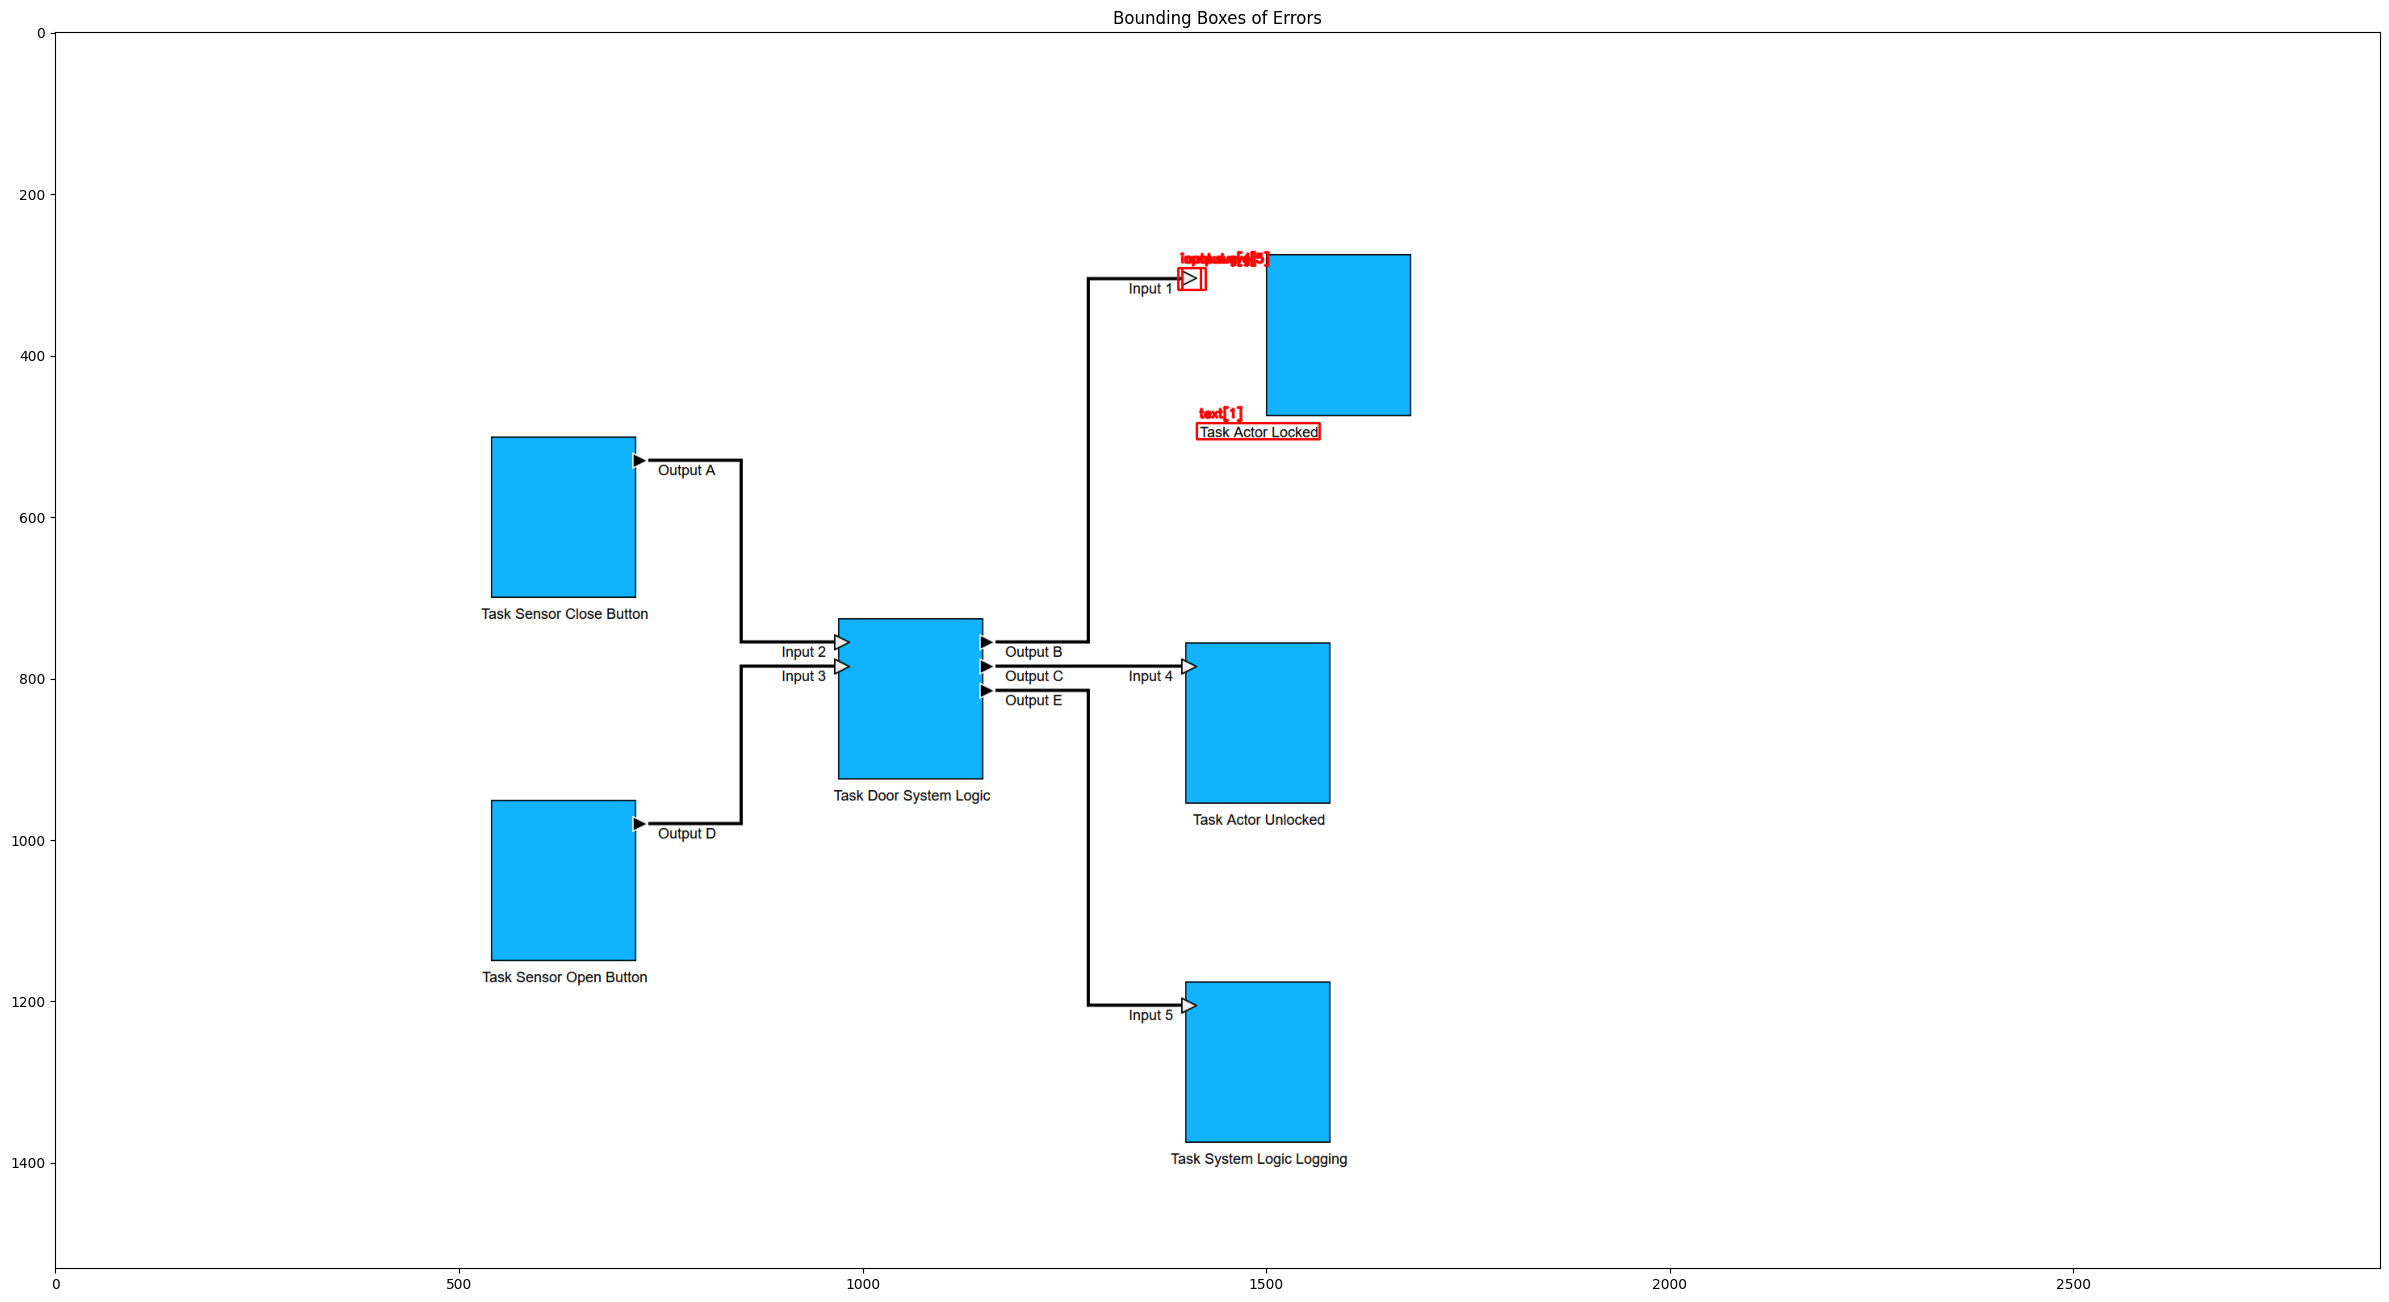
\includegraphics[width=\textwidth]{testcases/vertex_task_wrong_position/134550-162424_element_bbox_errors_labeled_colored.png}
        \caption*{\textit{After}}
    \end{subfigure}
    % \caption{Vertex in model, but not in visualization}
    \label{fig:vertex_task_wrong_position}
\end{figure}
\newpage

\section{Vertices too close to each other}
\begin{figure}[H]
    \centering
    \begin{subfigure}[t]{0.9\textwidth}
        \centering
        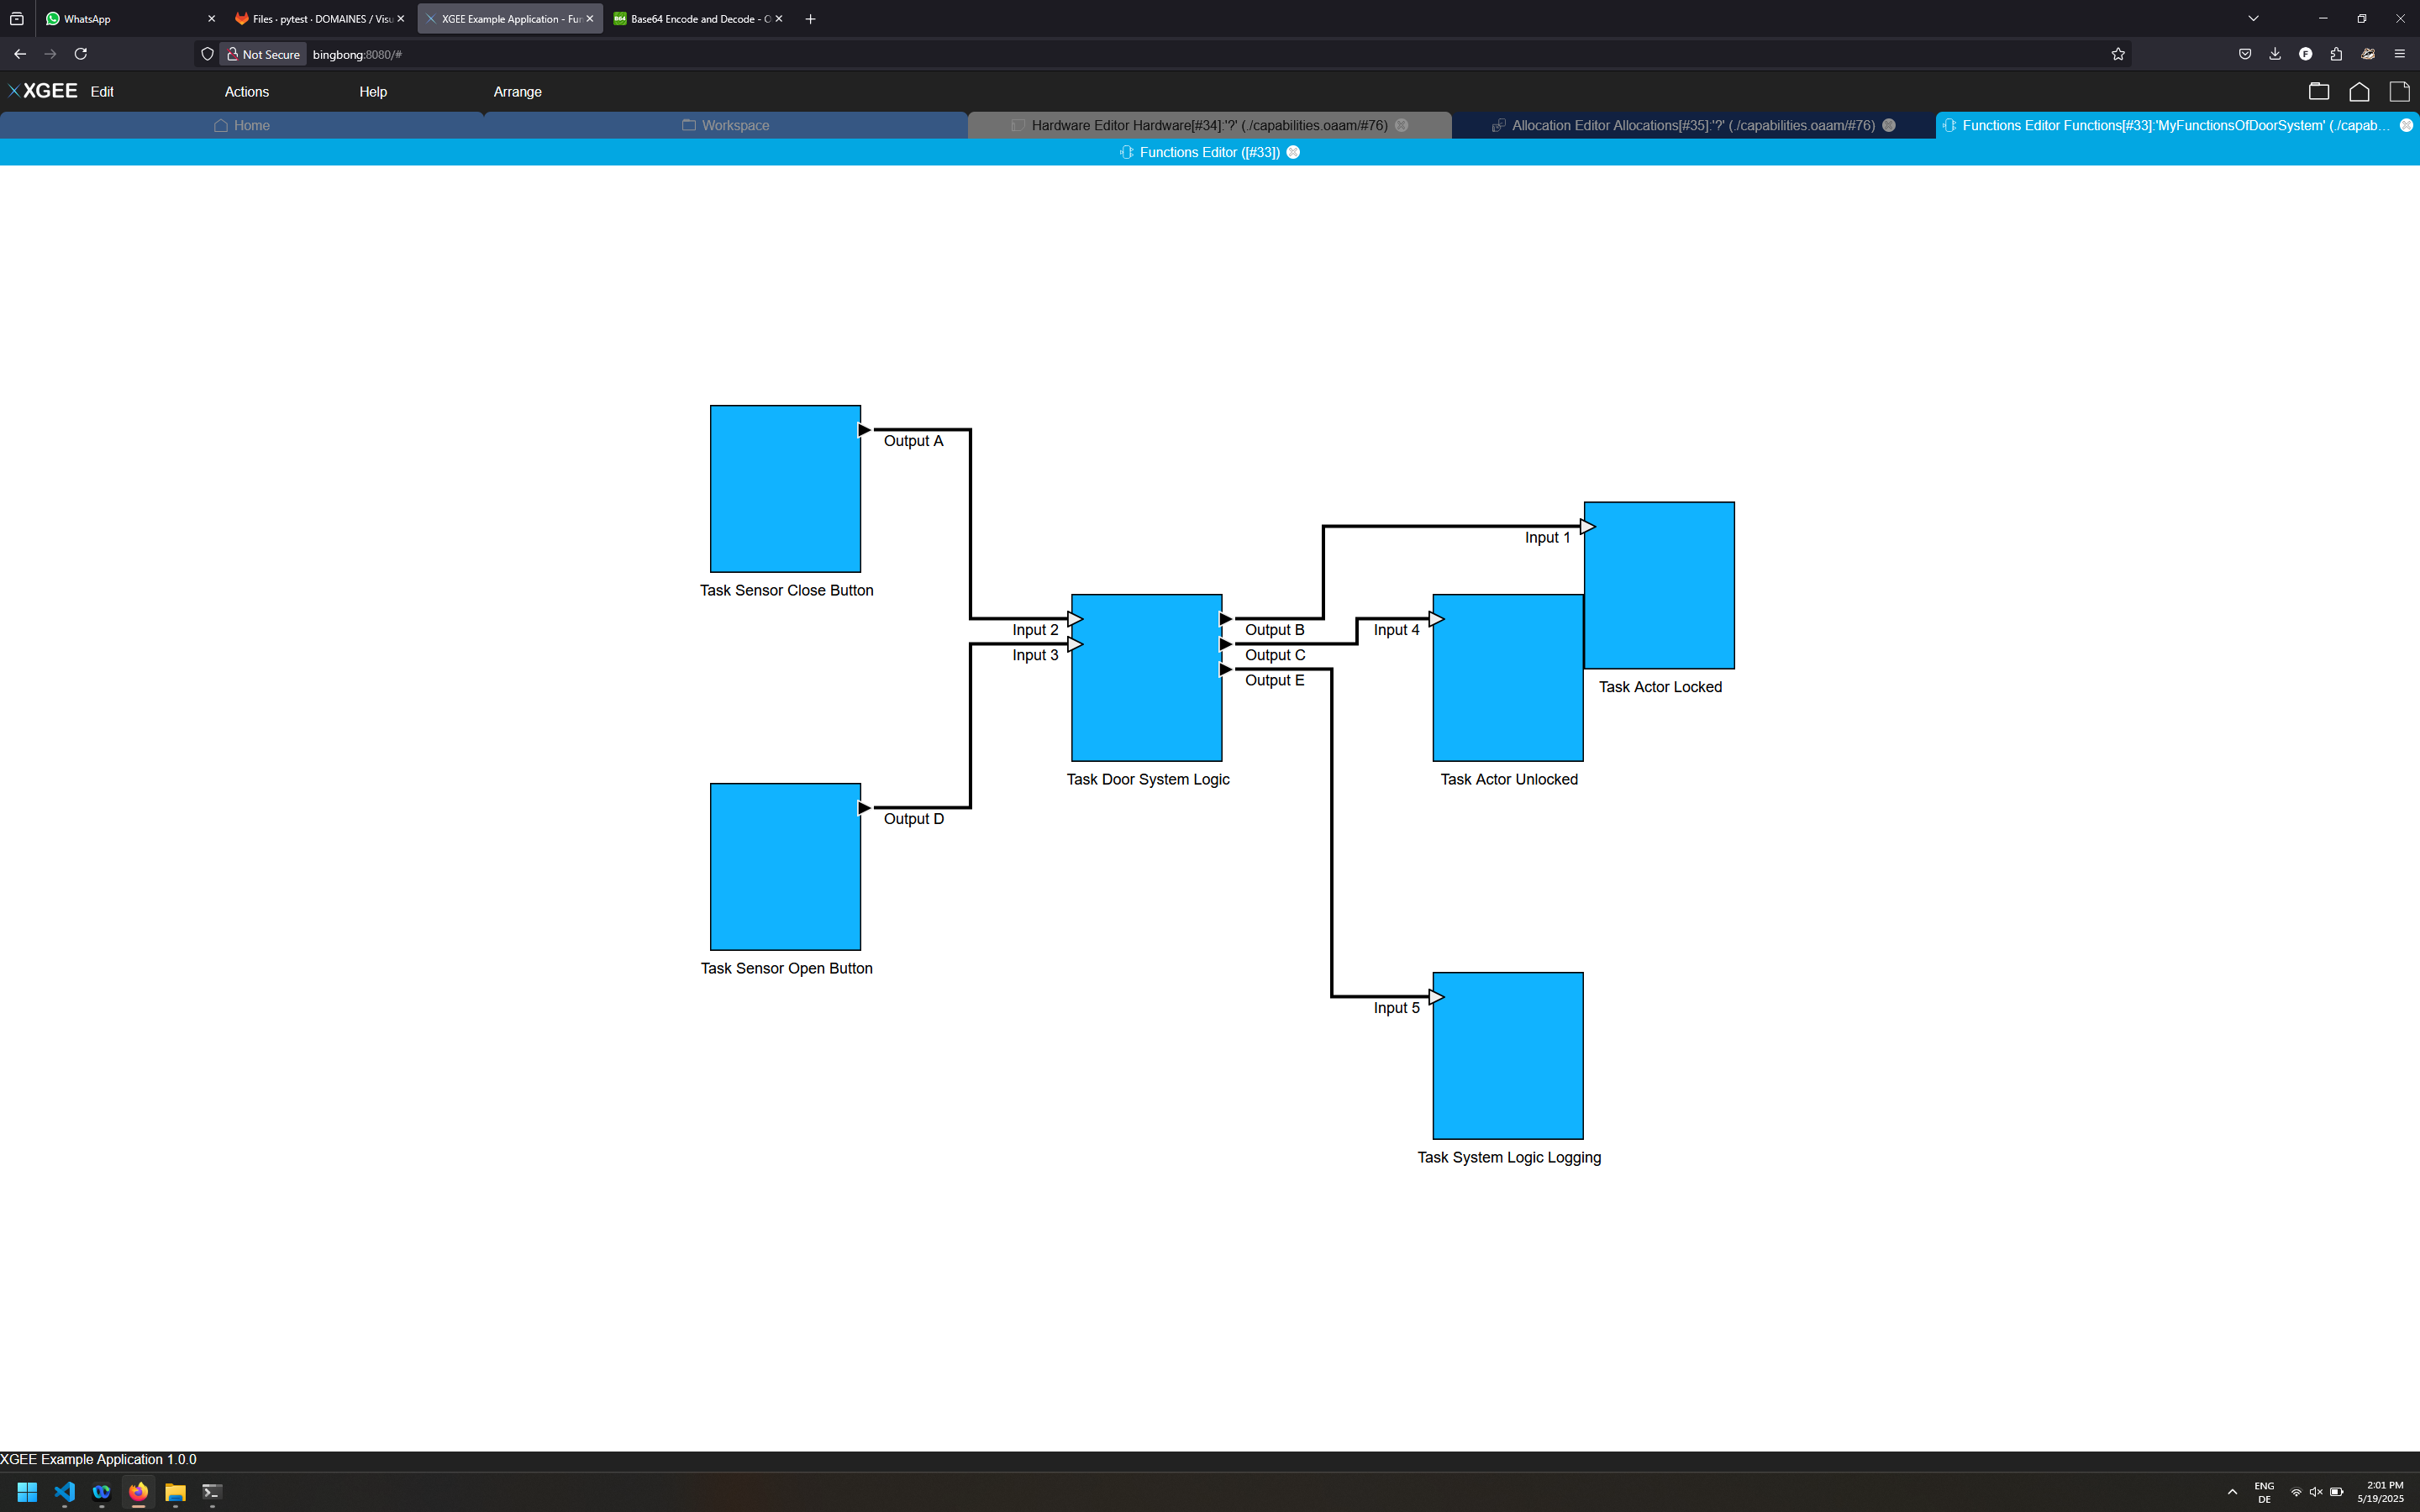
\includegraphics[width=\textwidth]{testcases/vertices_too_close/140151-897377_input_image.png}
        \caption*{\textit{Before}}
    \end{subfigure}
    \newline
    \begin{subfigure}[t]{0.9\textwidth}
        \centering
        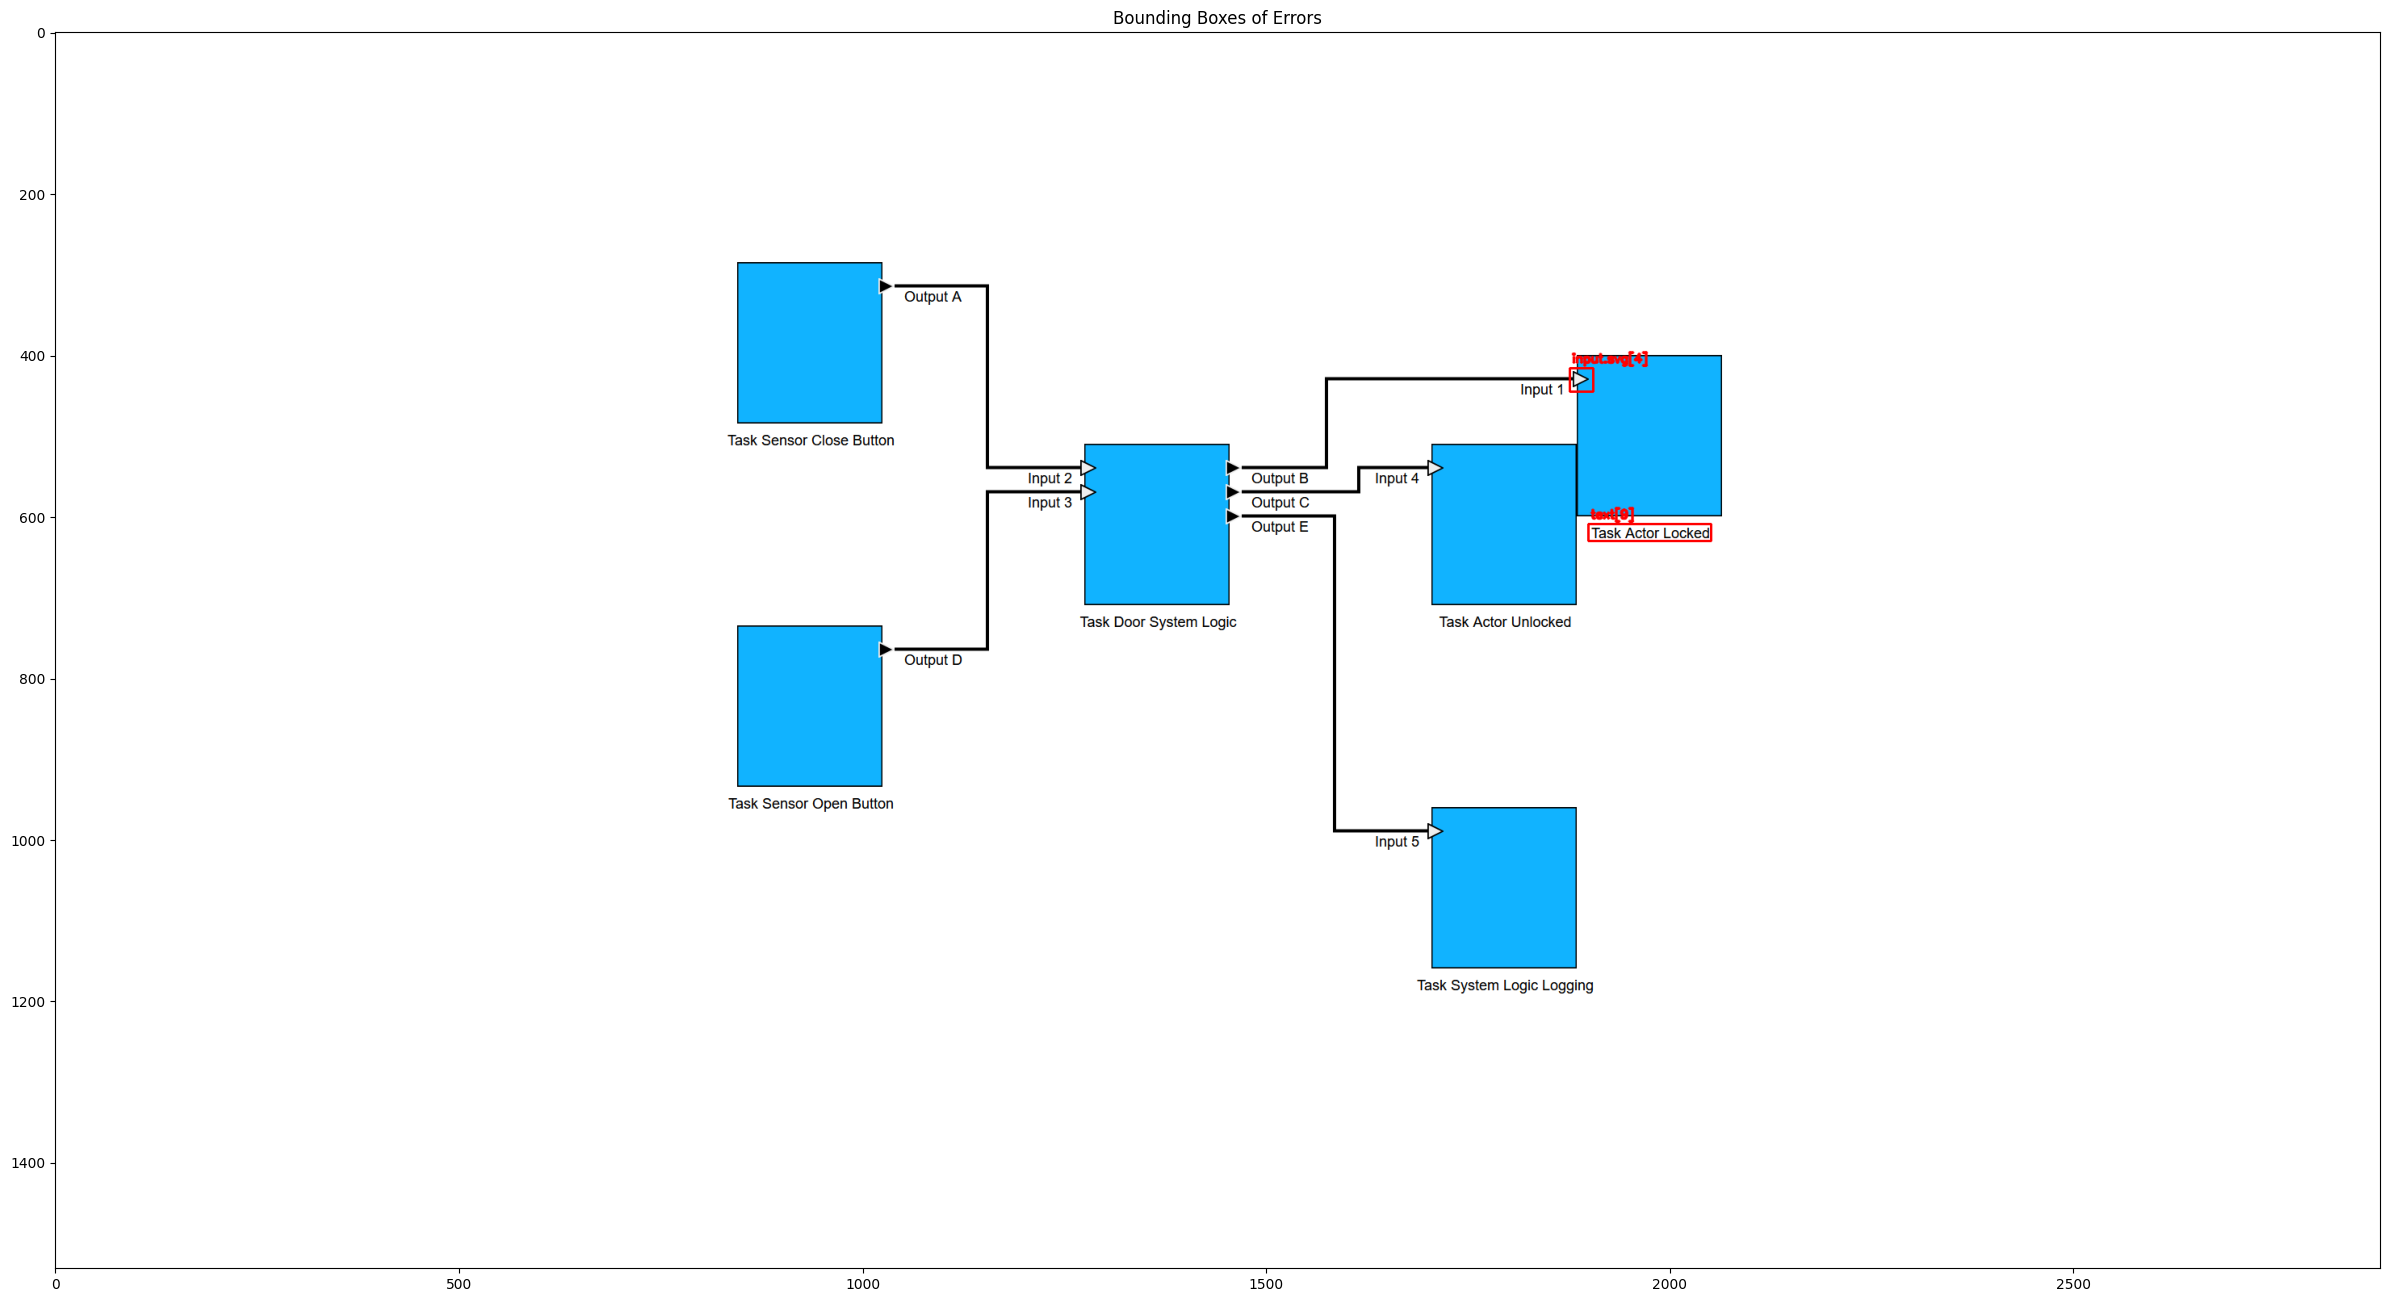
\includegraphics[width=\textwidth]{testcases/vertices_too_close/140211-889490_element_bbox_errors_labeled_colored.png}
        \caption*{\textit{After}}
    \end{subfigure}
    % \caption{Vertices too close to each other}
    \label{fig:vertices_too_close}
\end{figure}
\newpage

\section{Vertices overlapping}
\begin{figure}[H]
    \centering
    \begin{subfigure}[t]{0.9\textwidth}
        \centering
        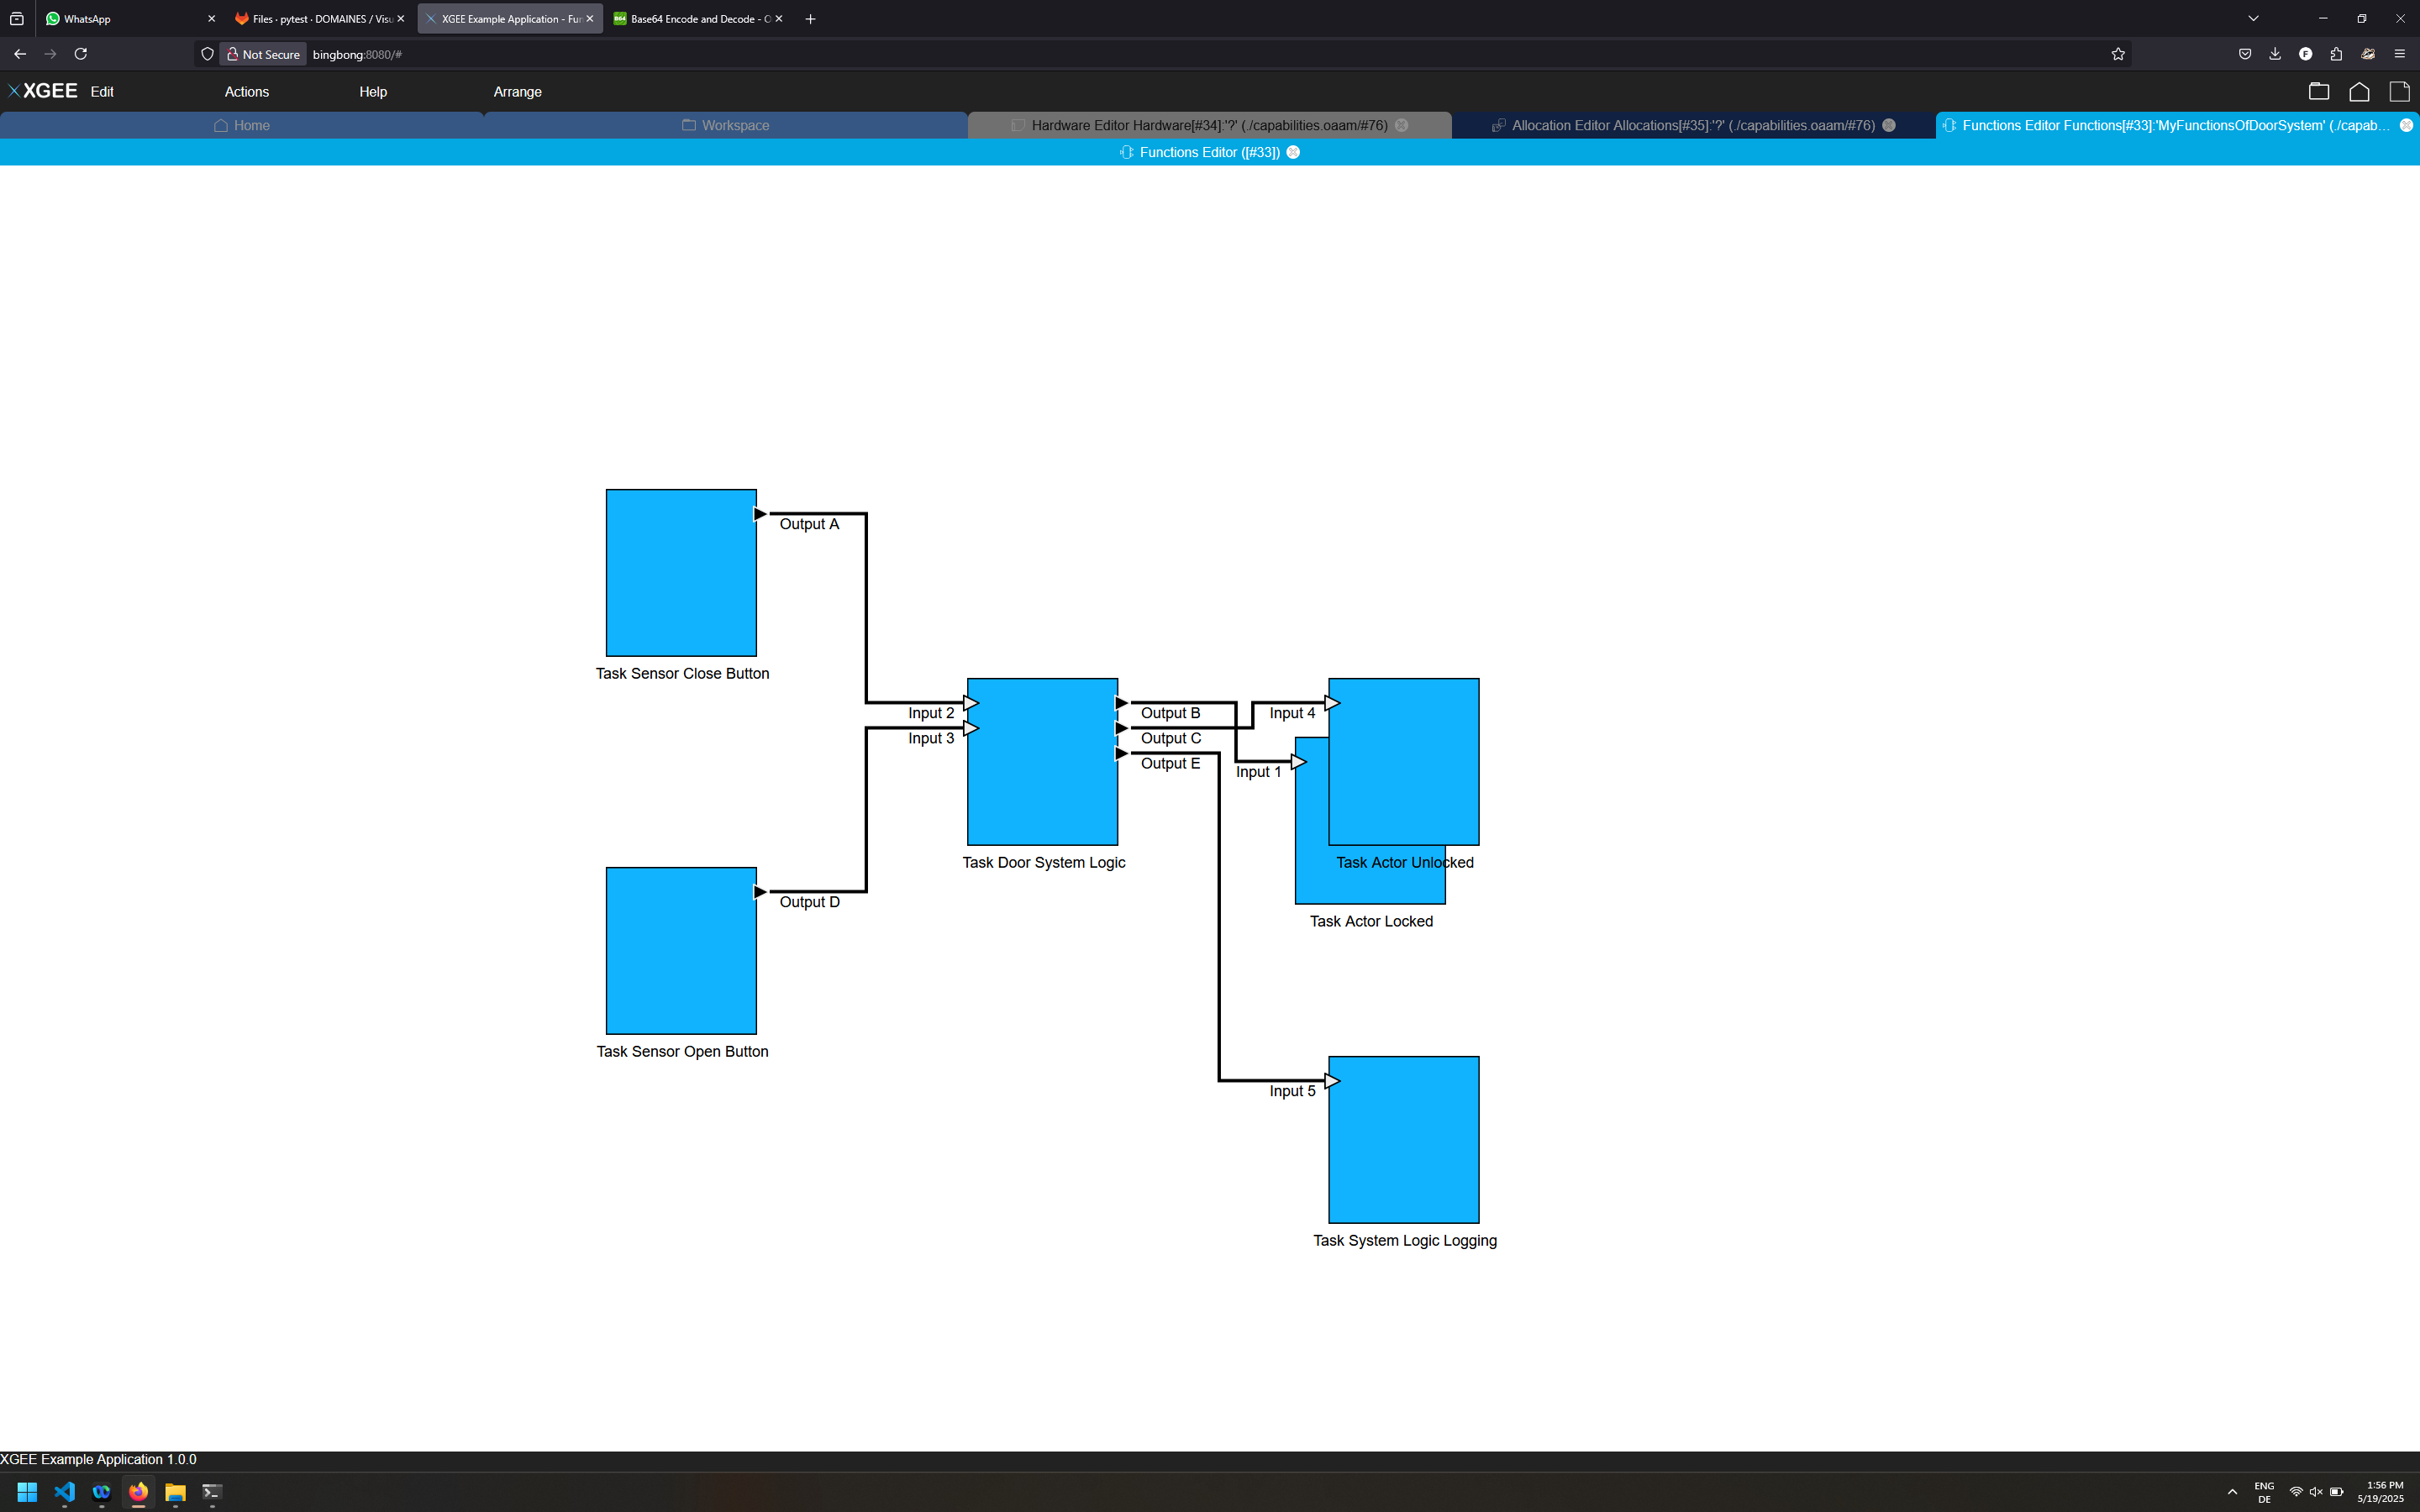
\includegraphics[width=\textwidth]{testcases/vertices_overlapping/135655-256834_input_image.png}
        \caption*{\textit{Before}}
    \end{subfigure}
    \newline
    \begin{subfigure}[t]{0.9\textwidth}
        \centering
        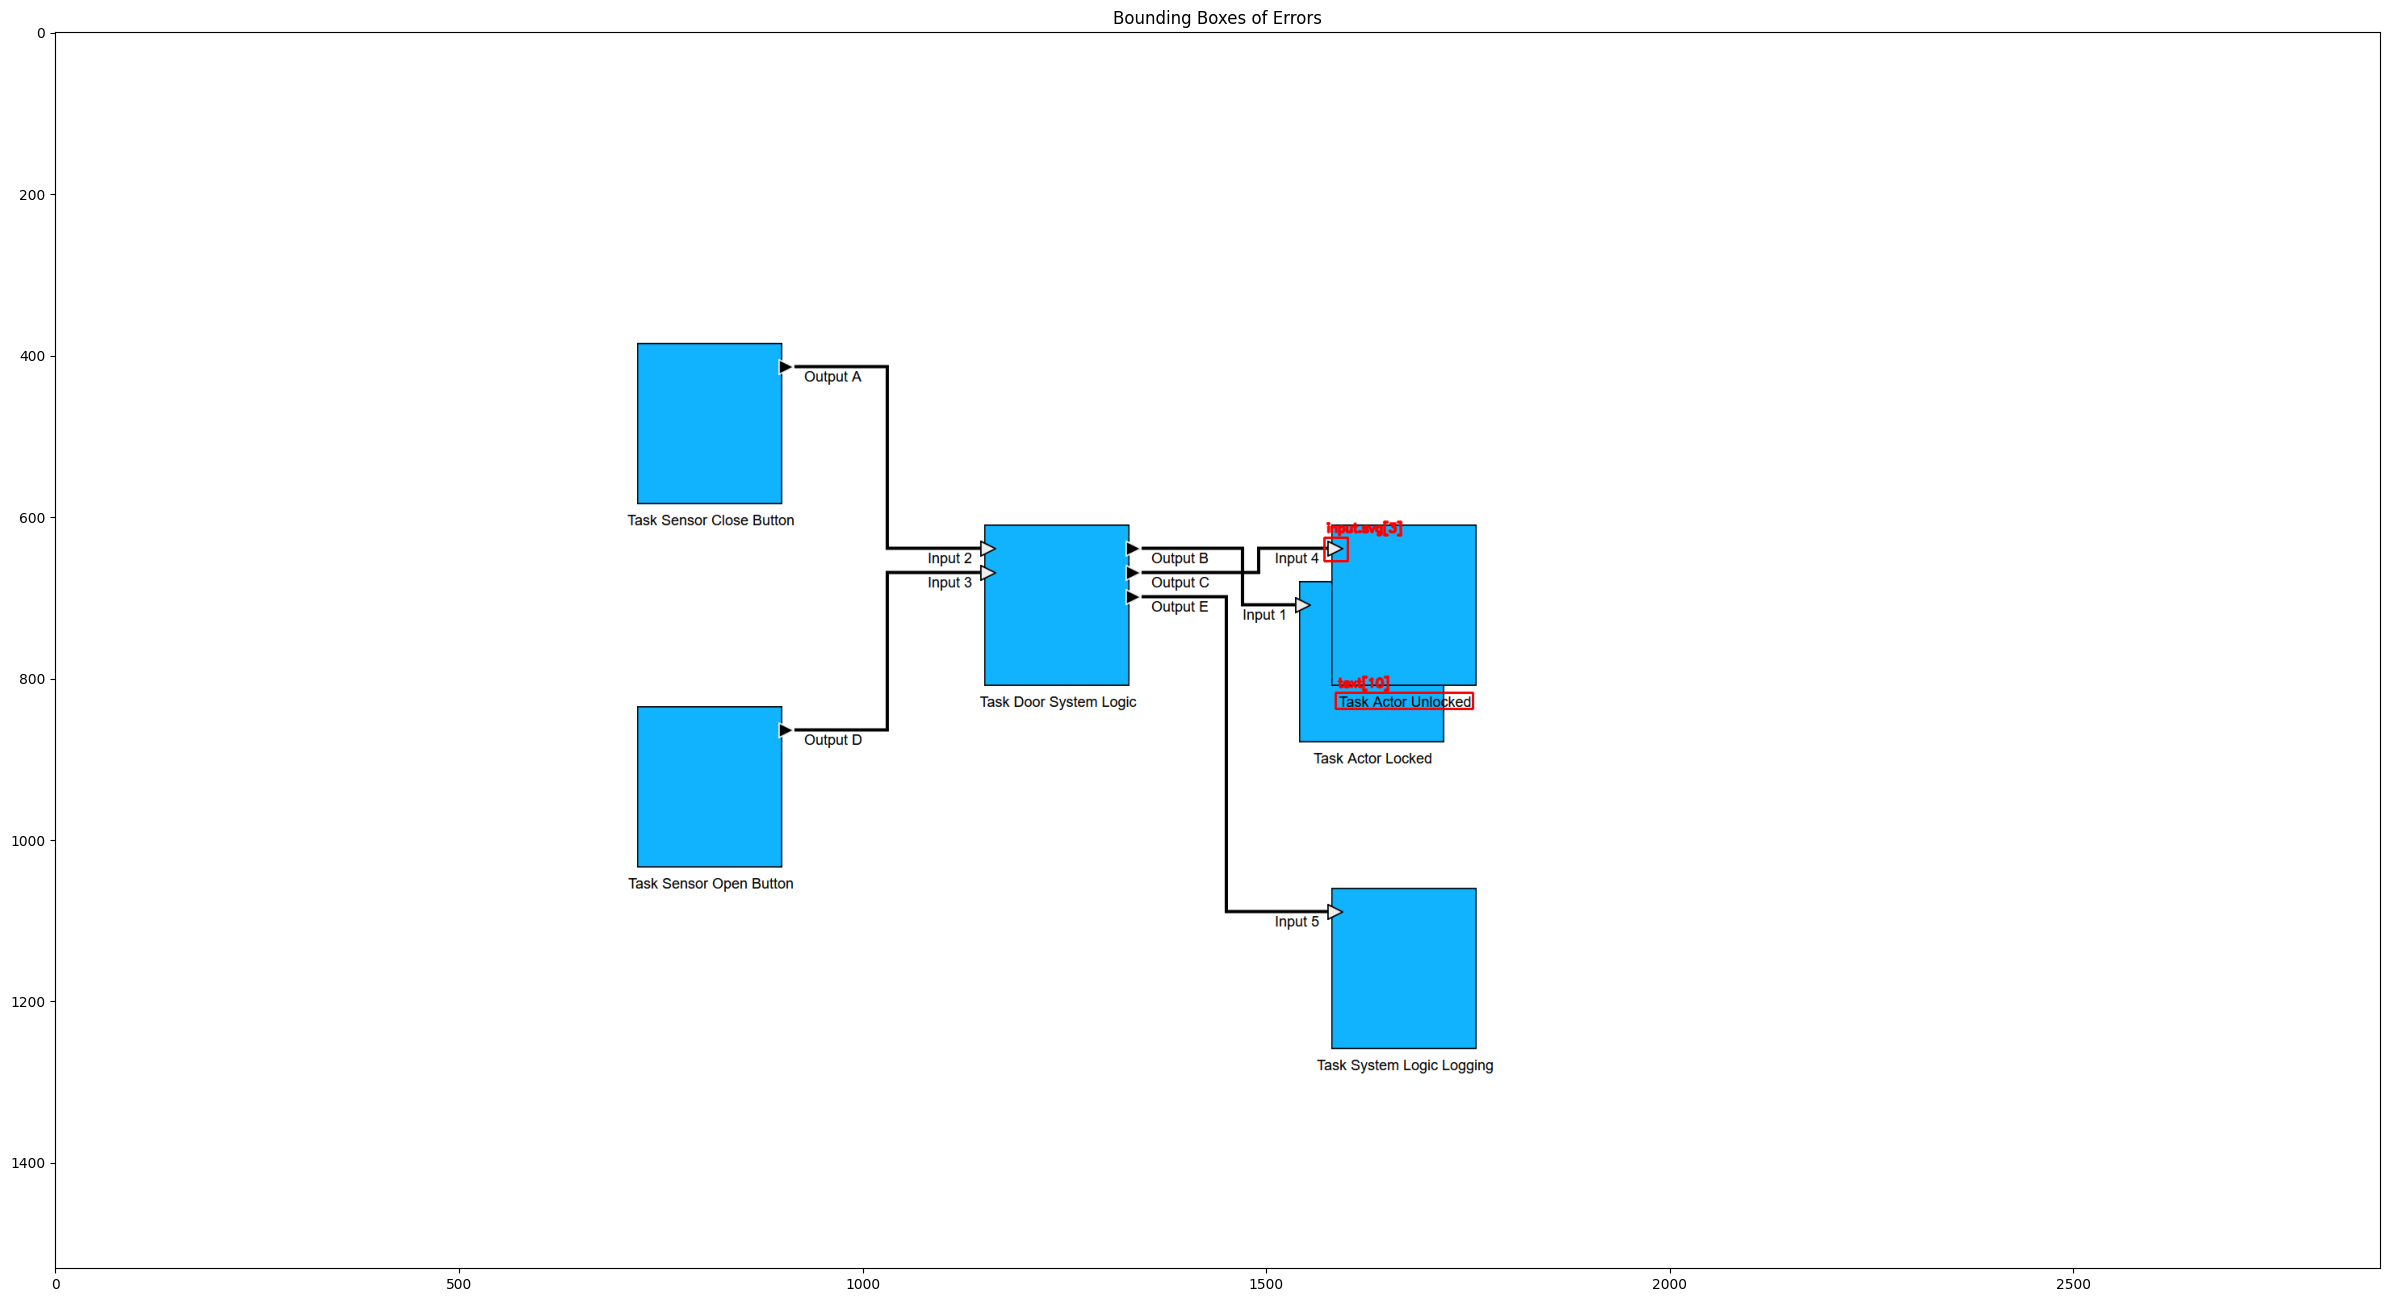
\includegraphics[width=\textwidth]{testcases/vertices_overlapping/135714-844562_element_bbox_errors_labeled_colored.png}
        \caption*{\textit{After}}
    \end{subfigure}
    % \caption{Vertices overlapping}
    \label{fig:vertices_overlapping}
\end{figure}
\newpage

\section{Vertices Partly offscreen}
\begin{figure}[H]
    \centering
    \begin{subfigure}[t]{0.9\textwidth}
        \centering
        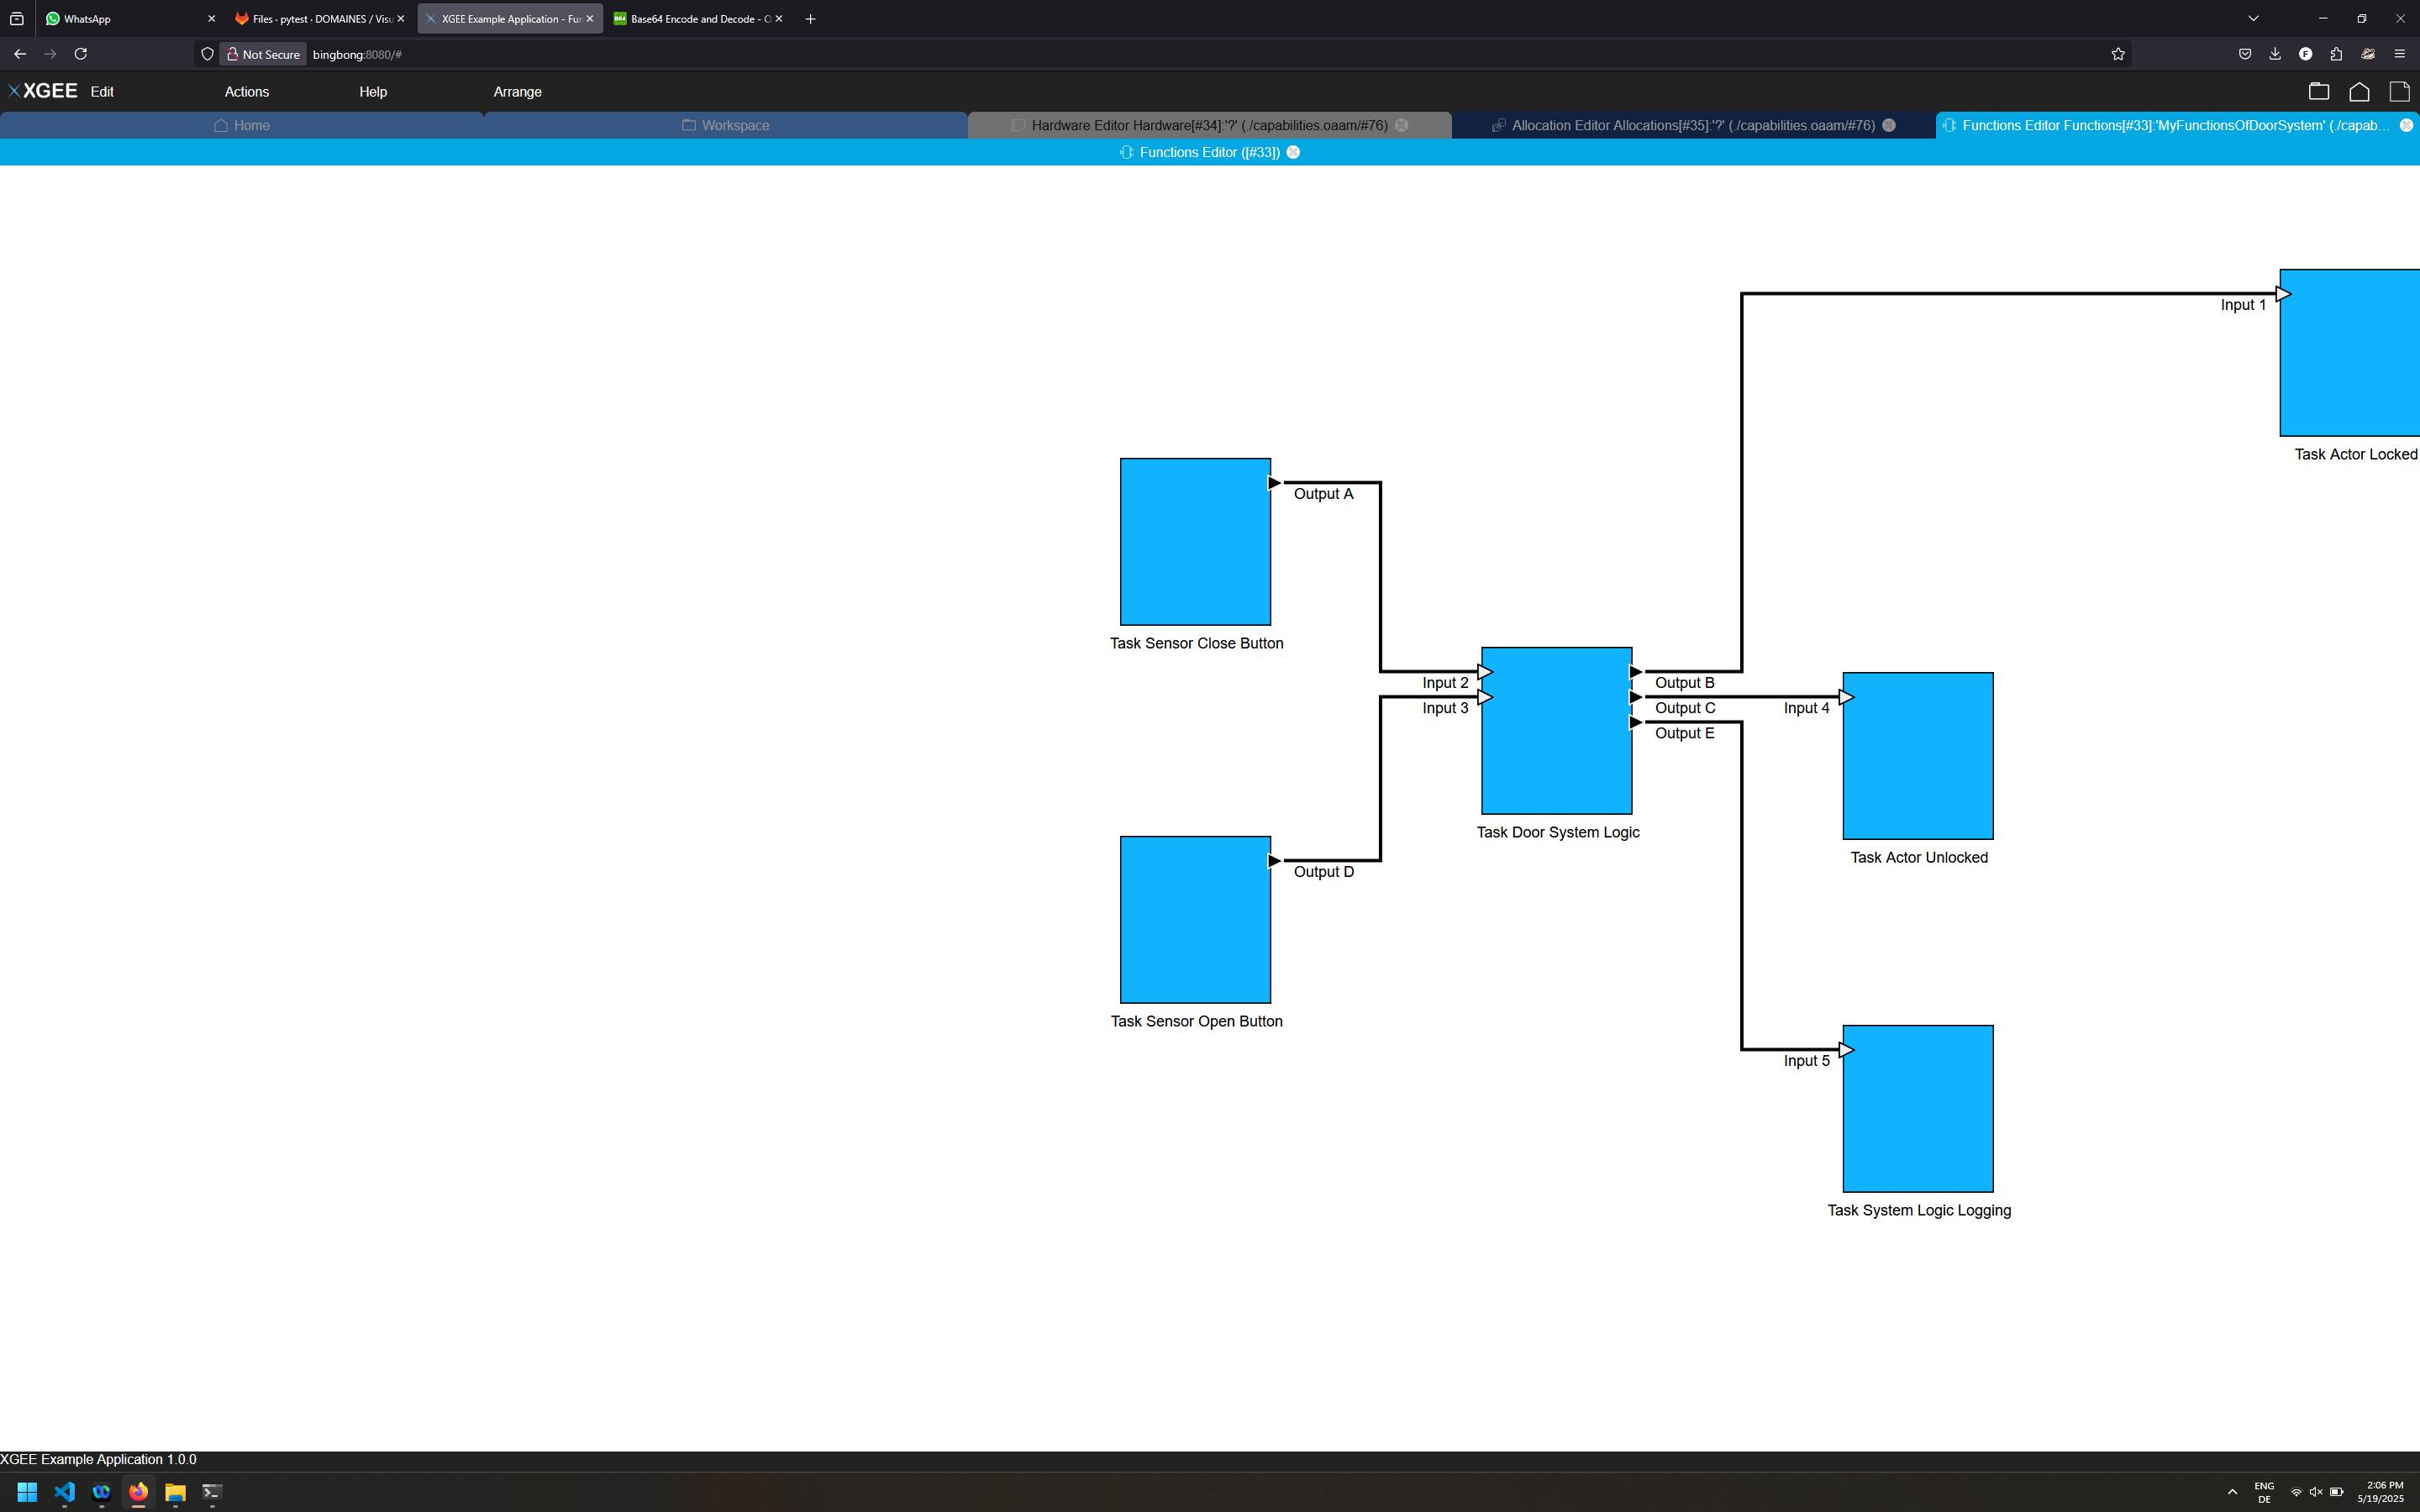
\includegraphics[width=\textwidth]{testcases/vertex_offscreen_partly/140634-098602_input_image.png}
        \caption*{\textit{Before}}
    \end{subfigure}
    \newline
    \begin{subfigure}[t]{0.9\textwidth}
        \centering
        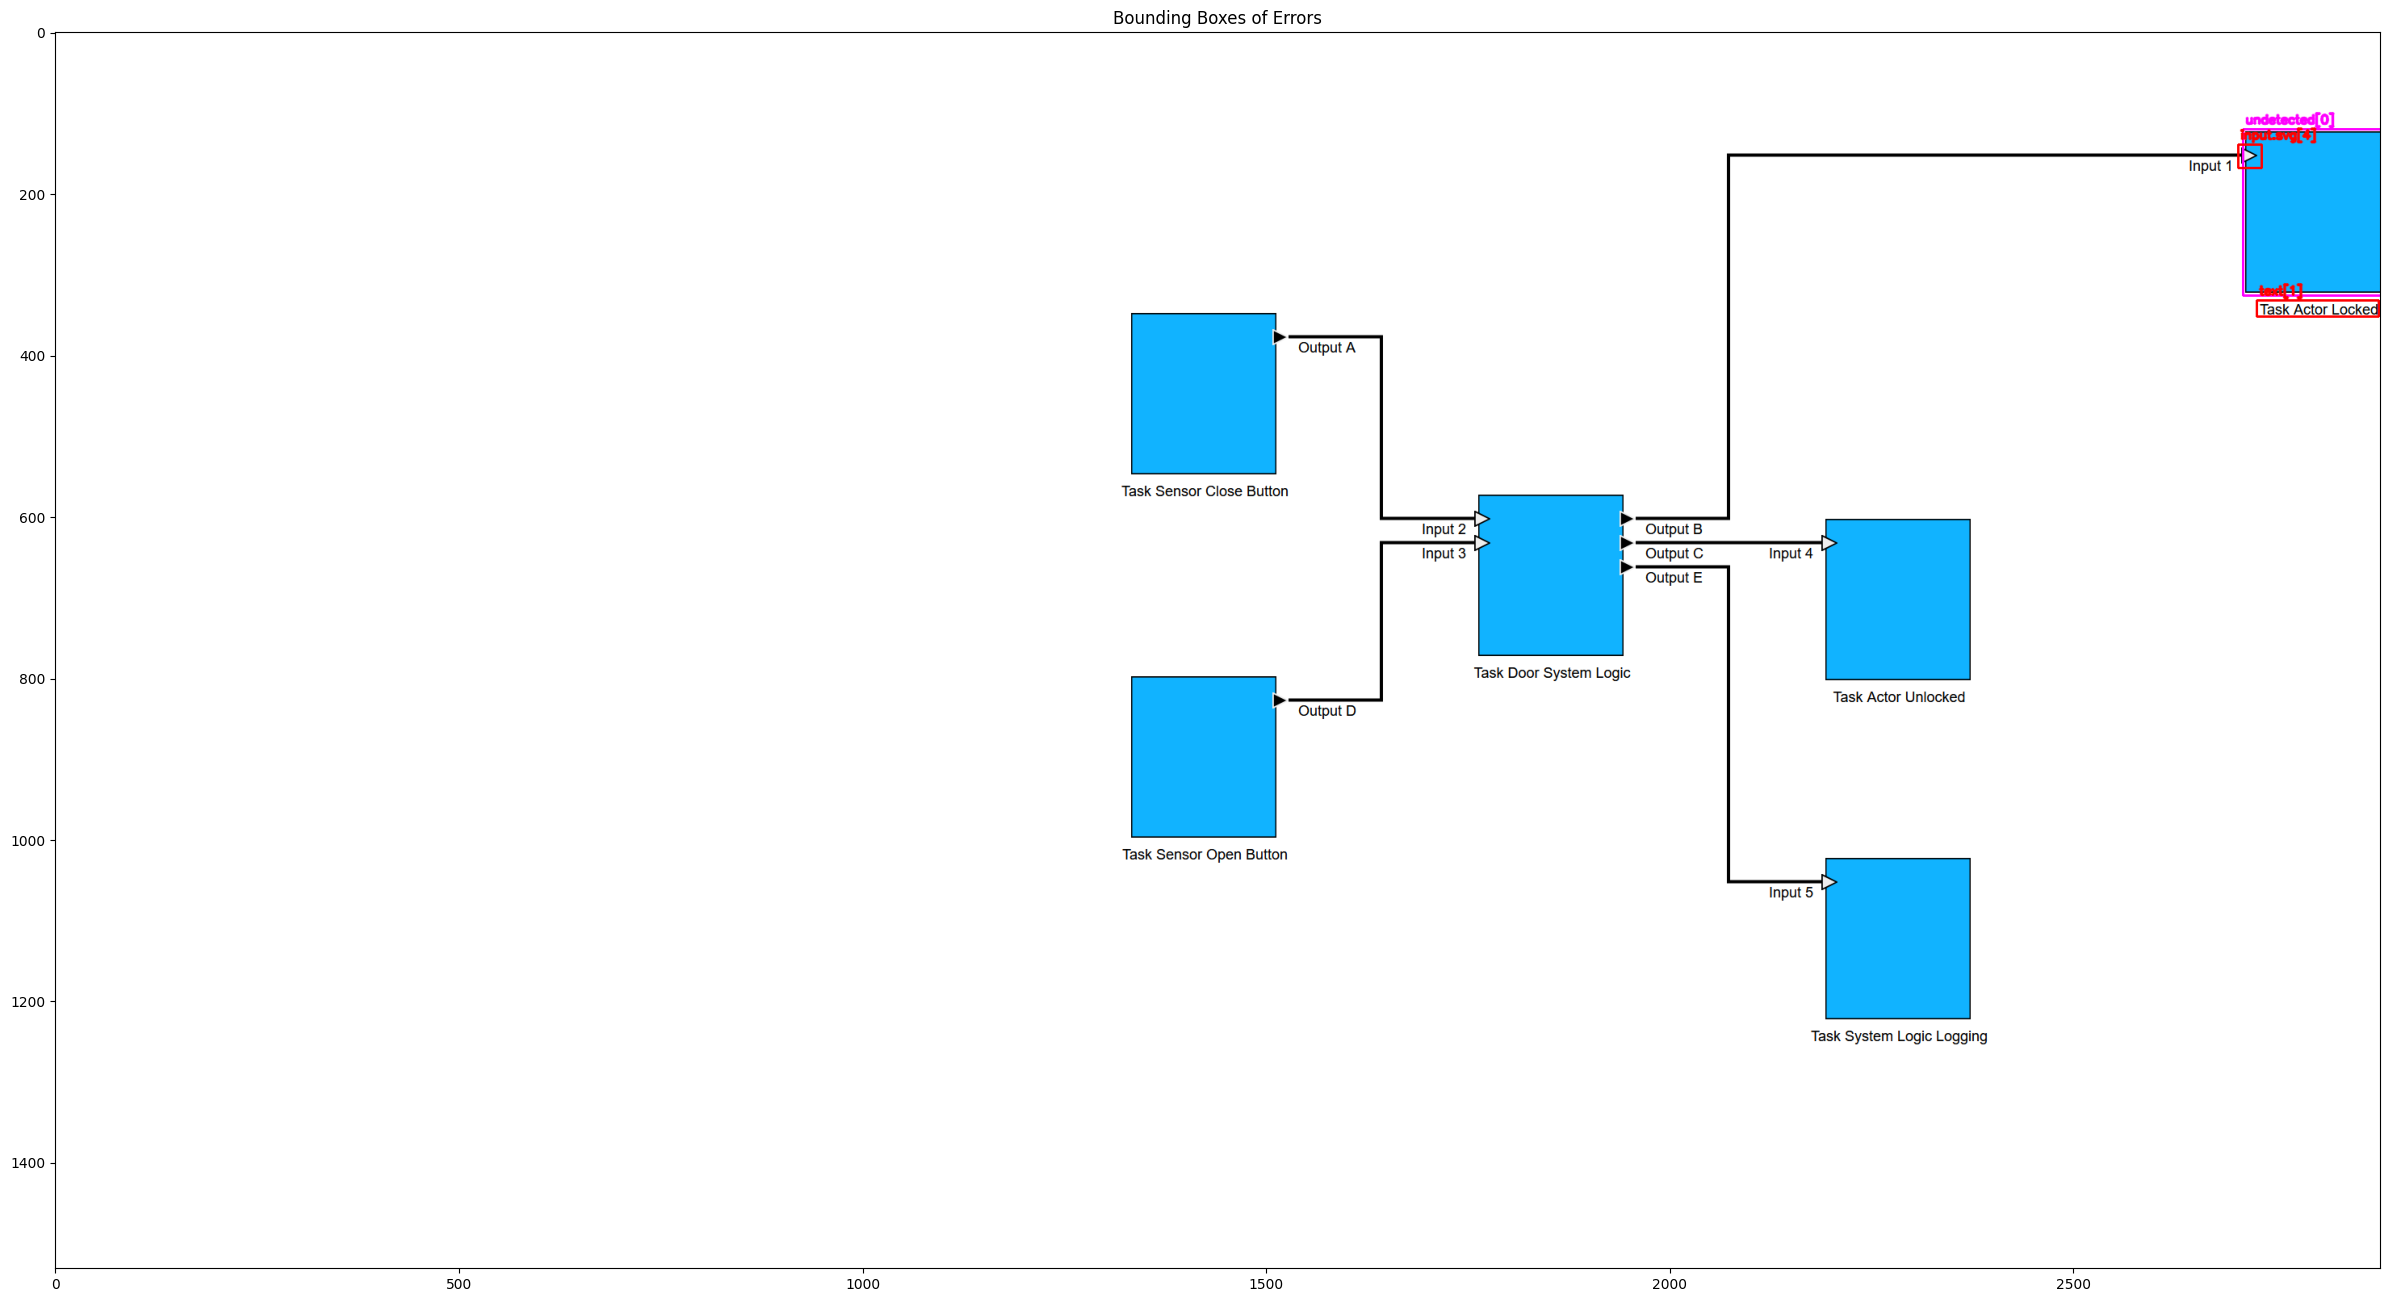
\includegraphics[width=\textwidth]{testcases/vertex_offscreen_partly/140653-729498_element_bbox_errors_labeled_colored.png}
        \caption*{\textit{After}}
    \end{subfigure}
    % \caption{Vertices offscreen}
    \label{fig:vertices_partly_offscreen}
\end{figure}
\newpage

\section{Vertices Completly offscreen}
\begin{figure}[H]
    \centering
    \begin{subfigure}[t]{0.9\textwidth}
        \centering
        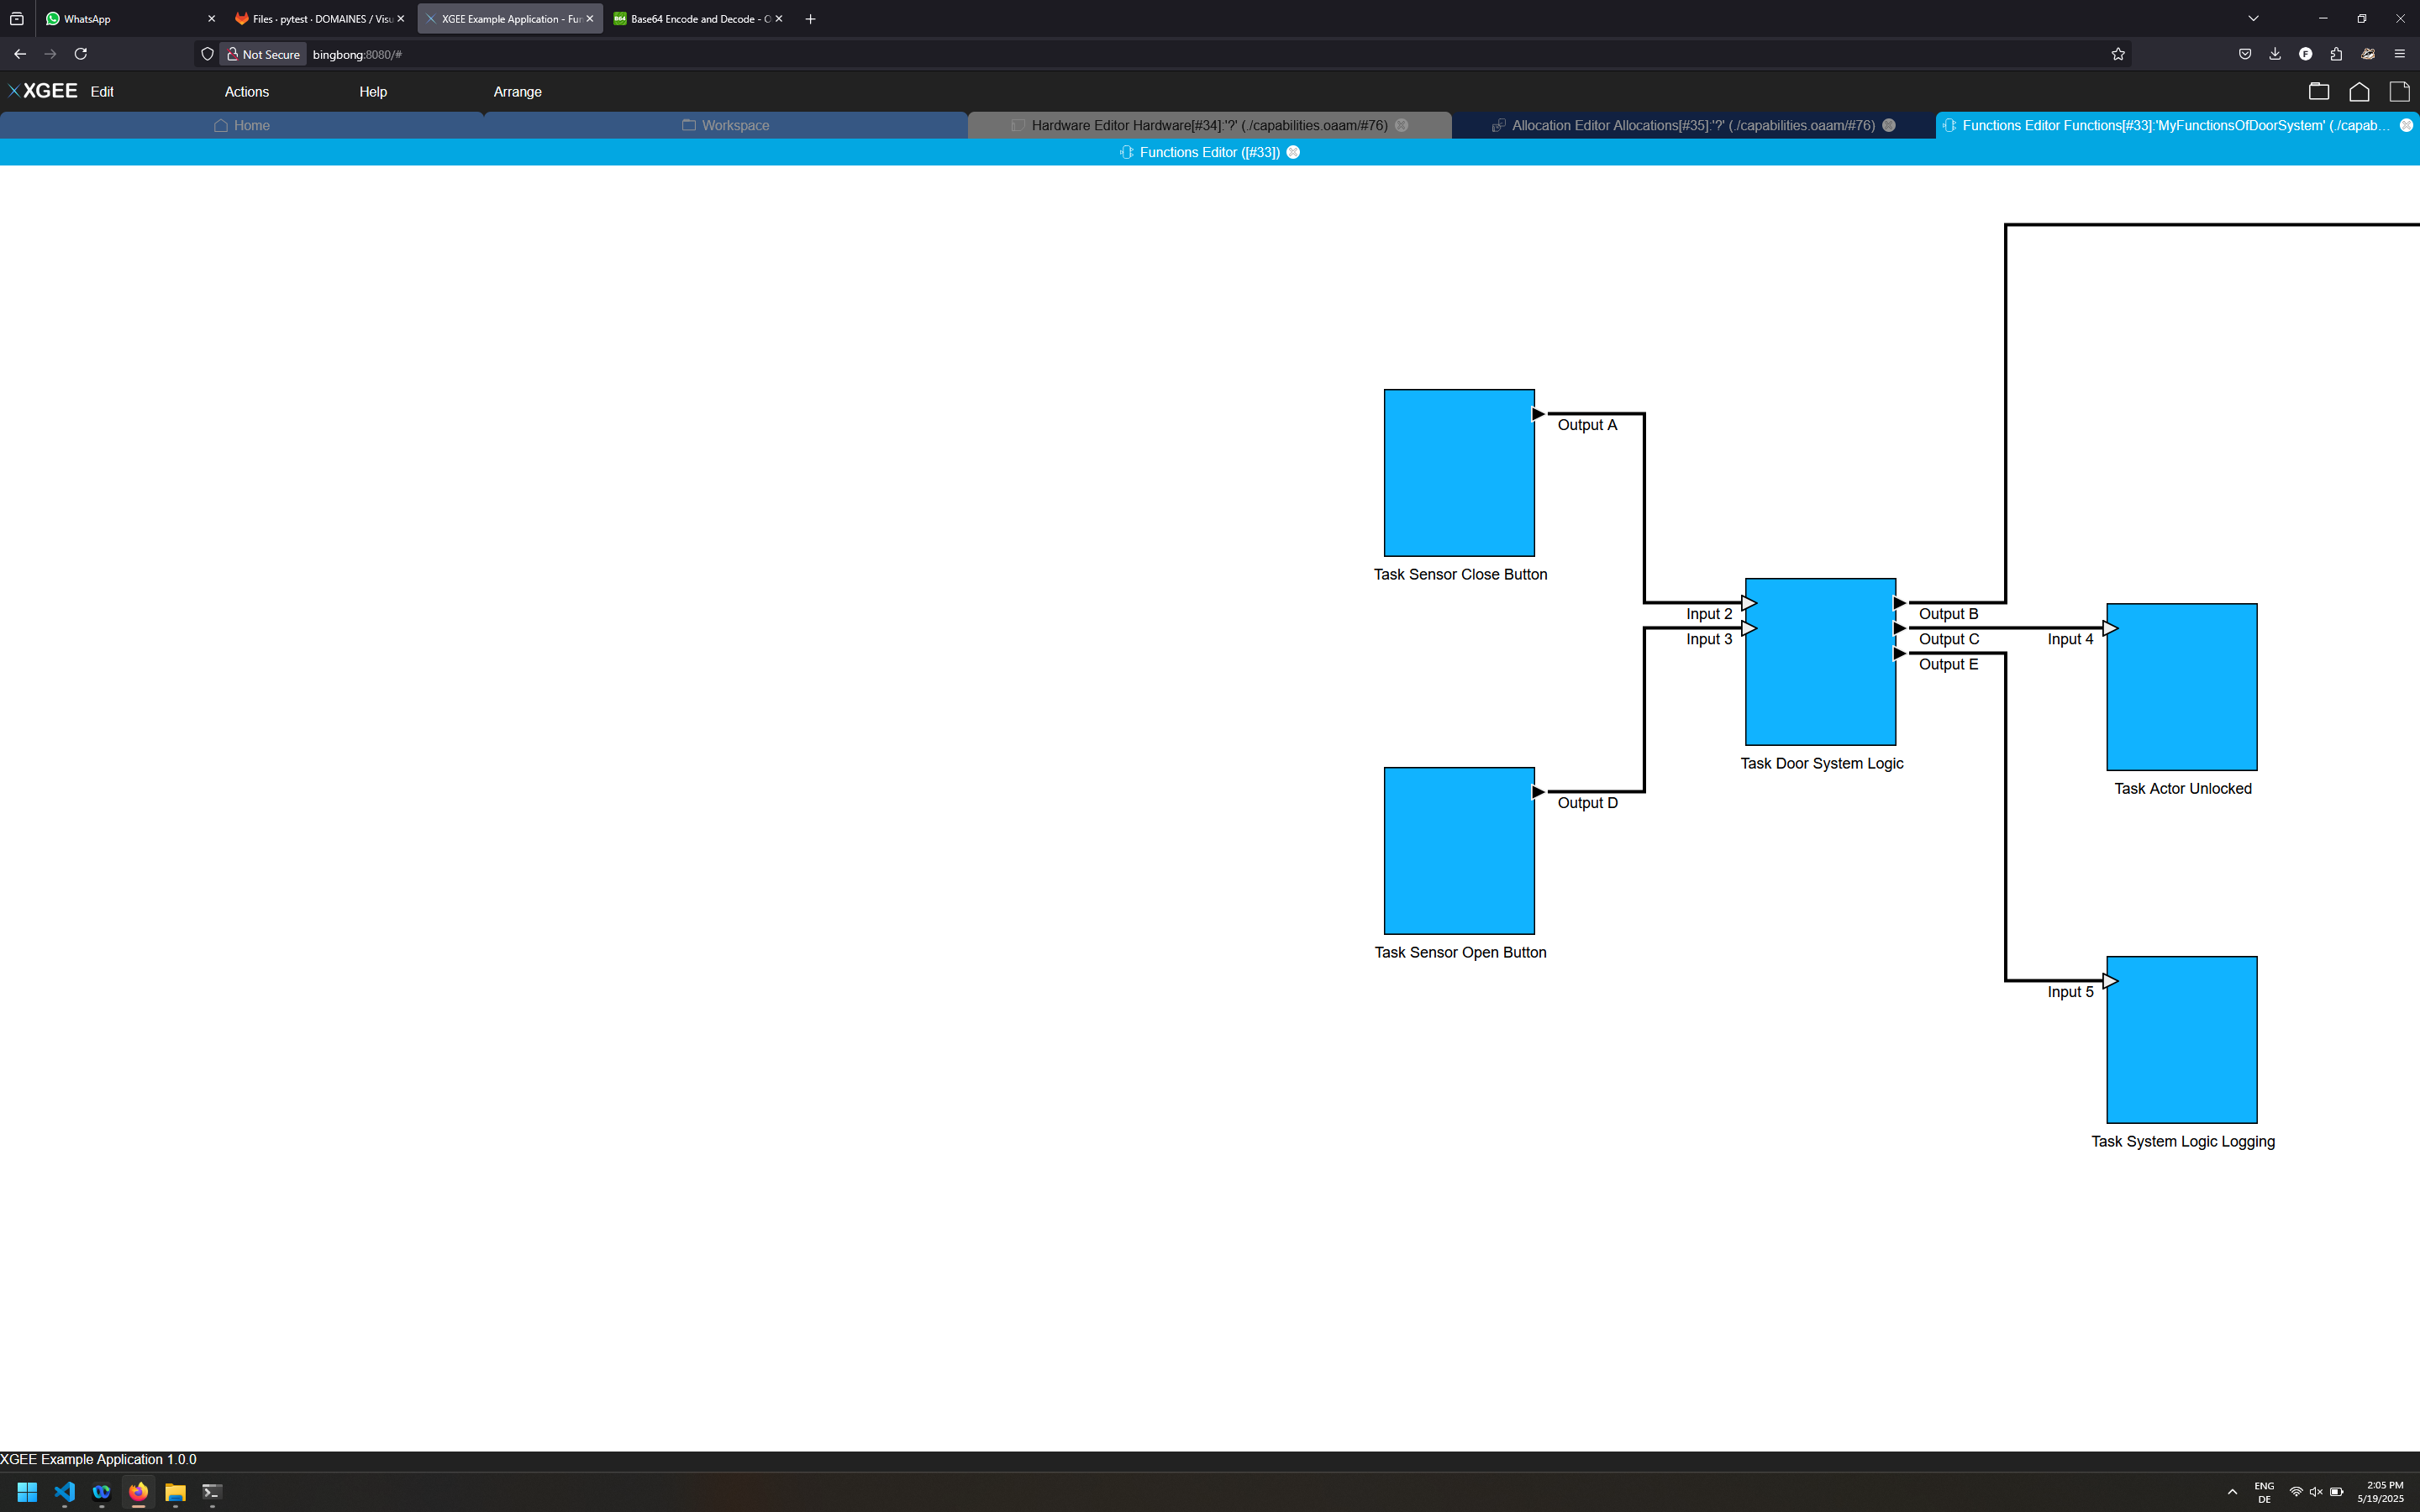
\includegraphics[width=\textwidth]{testcases/vertices_offscreen_completely/140516-946679_input_image.png}
        \caption*{\textit{Before}}
    \end{subfigure}
    \newline
    \begin{subfigure}[t]{0.9\textwidth}
        \centering
        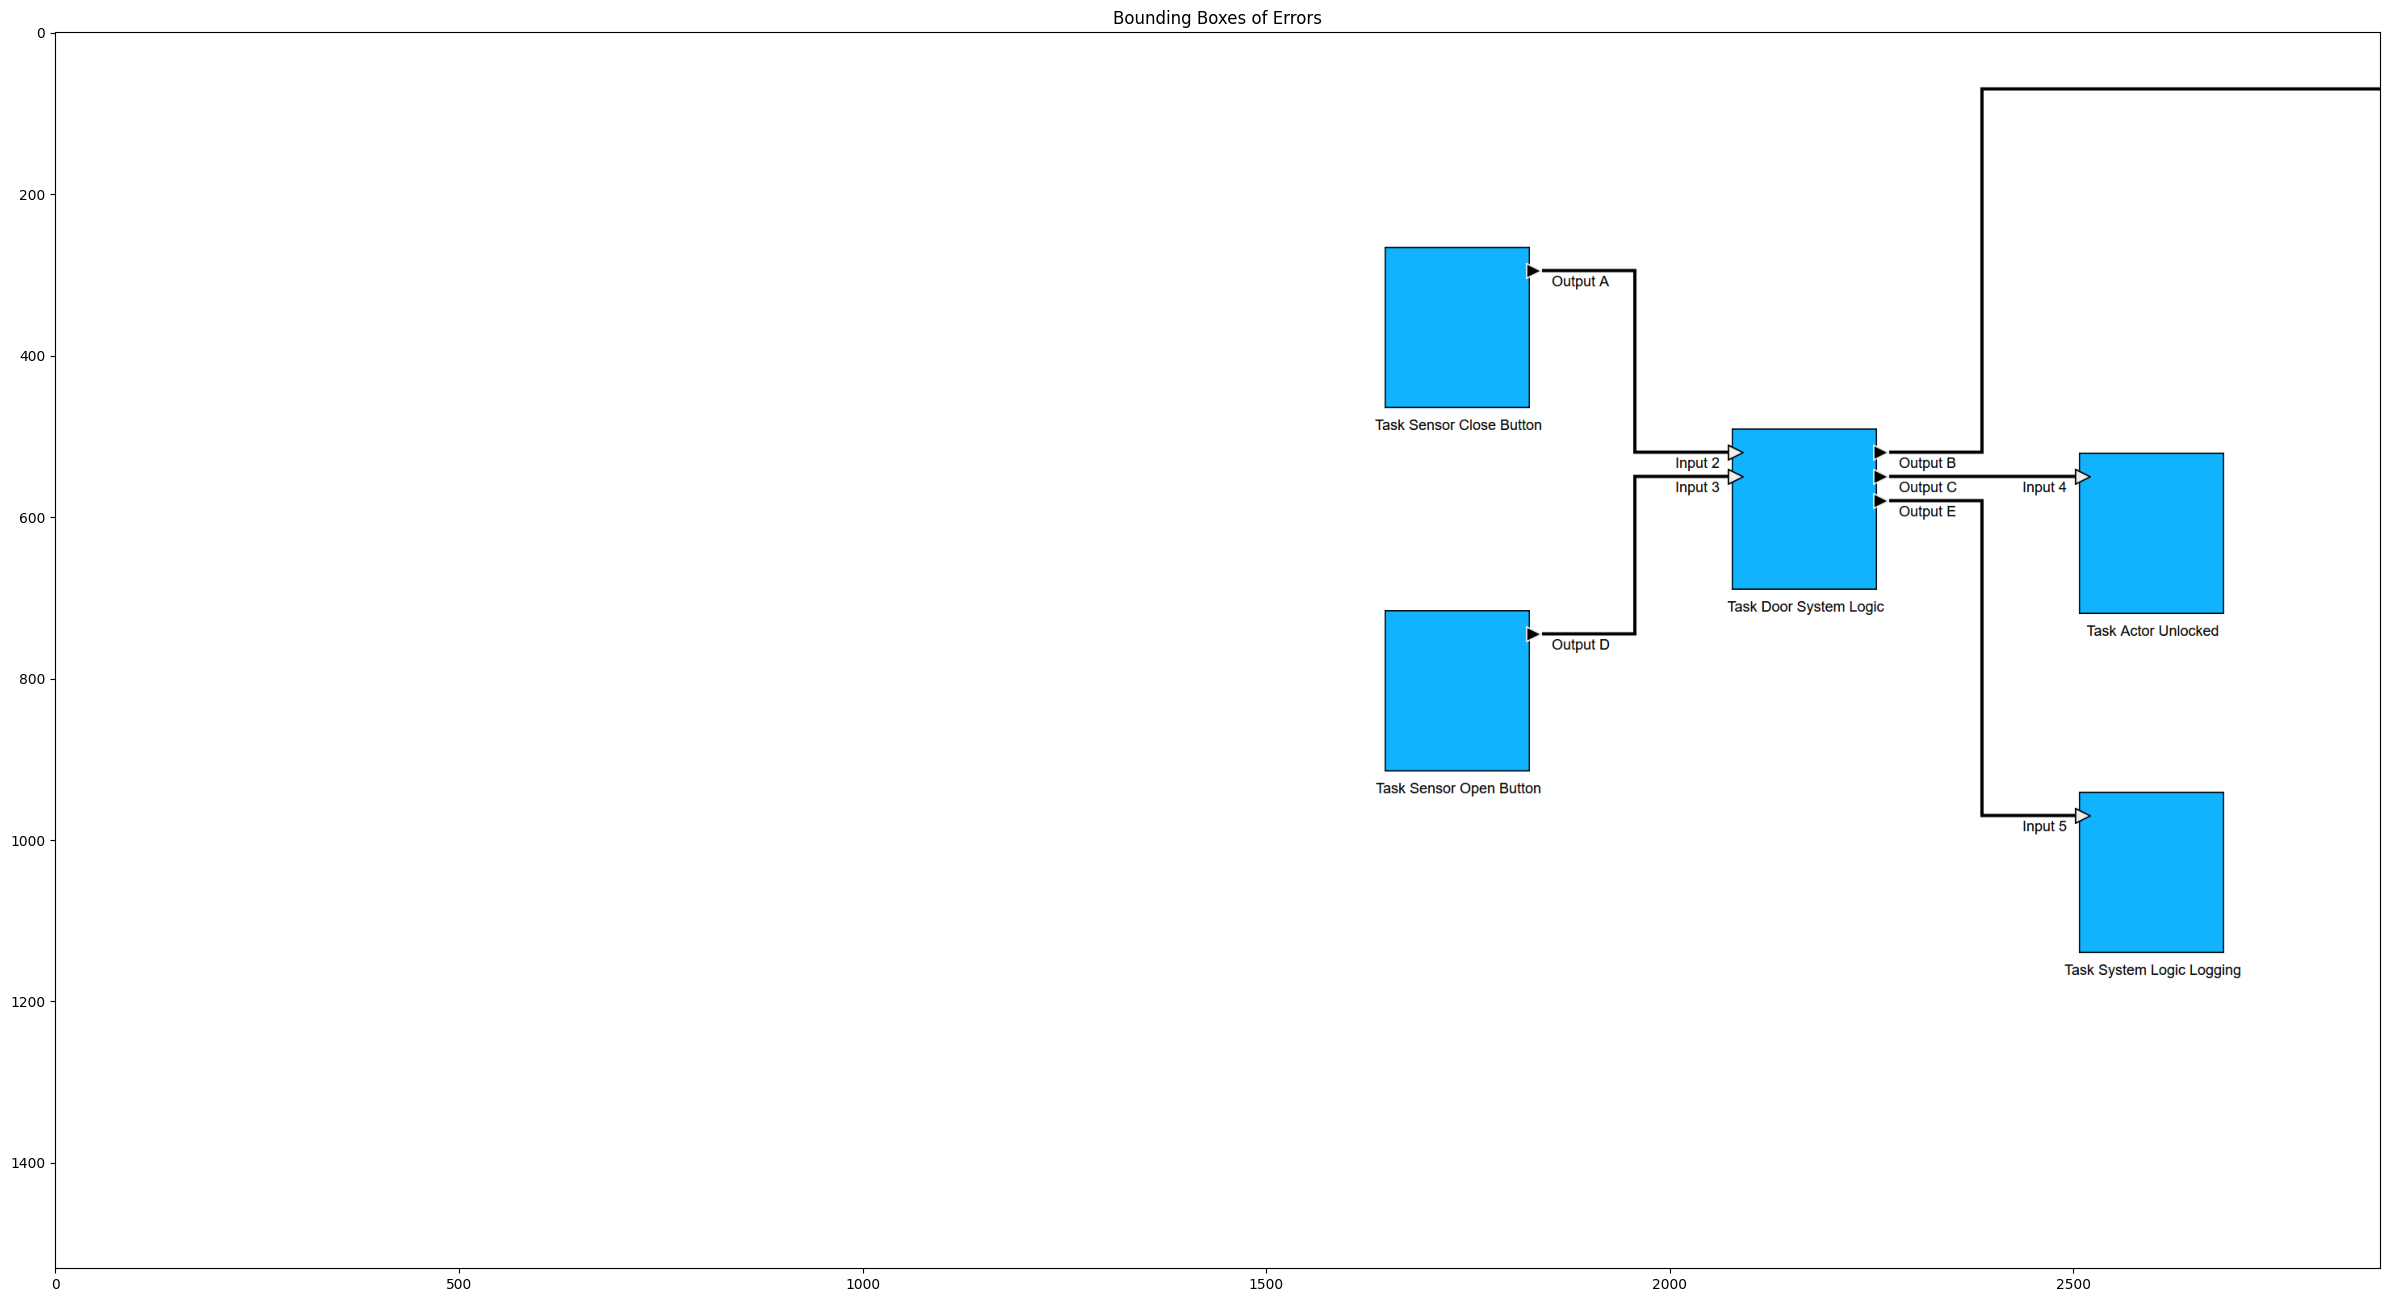
\includegraphics[width=\textwidth]{testcases/vertices_offscreen_completely/140536-824919_element_bbox_errors_labeled_colored.png}
        \caption*{\textit{After}}
    \end{subfigure}
    % \caption{Vertices offscreen}
    \label{fig:vertices_completly_offscreen}
\end{figure}
\newpage

\section{Vertex without parent element}
\begin{figure}[H]
    \centering
    \begin{subfigure}[t]{0.9\textwidth}
        \centering
        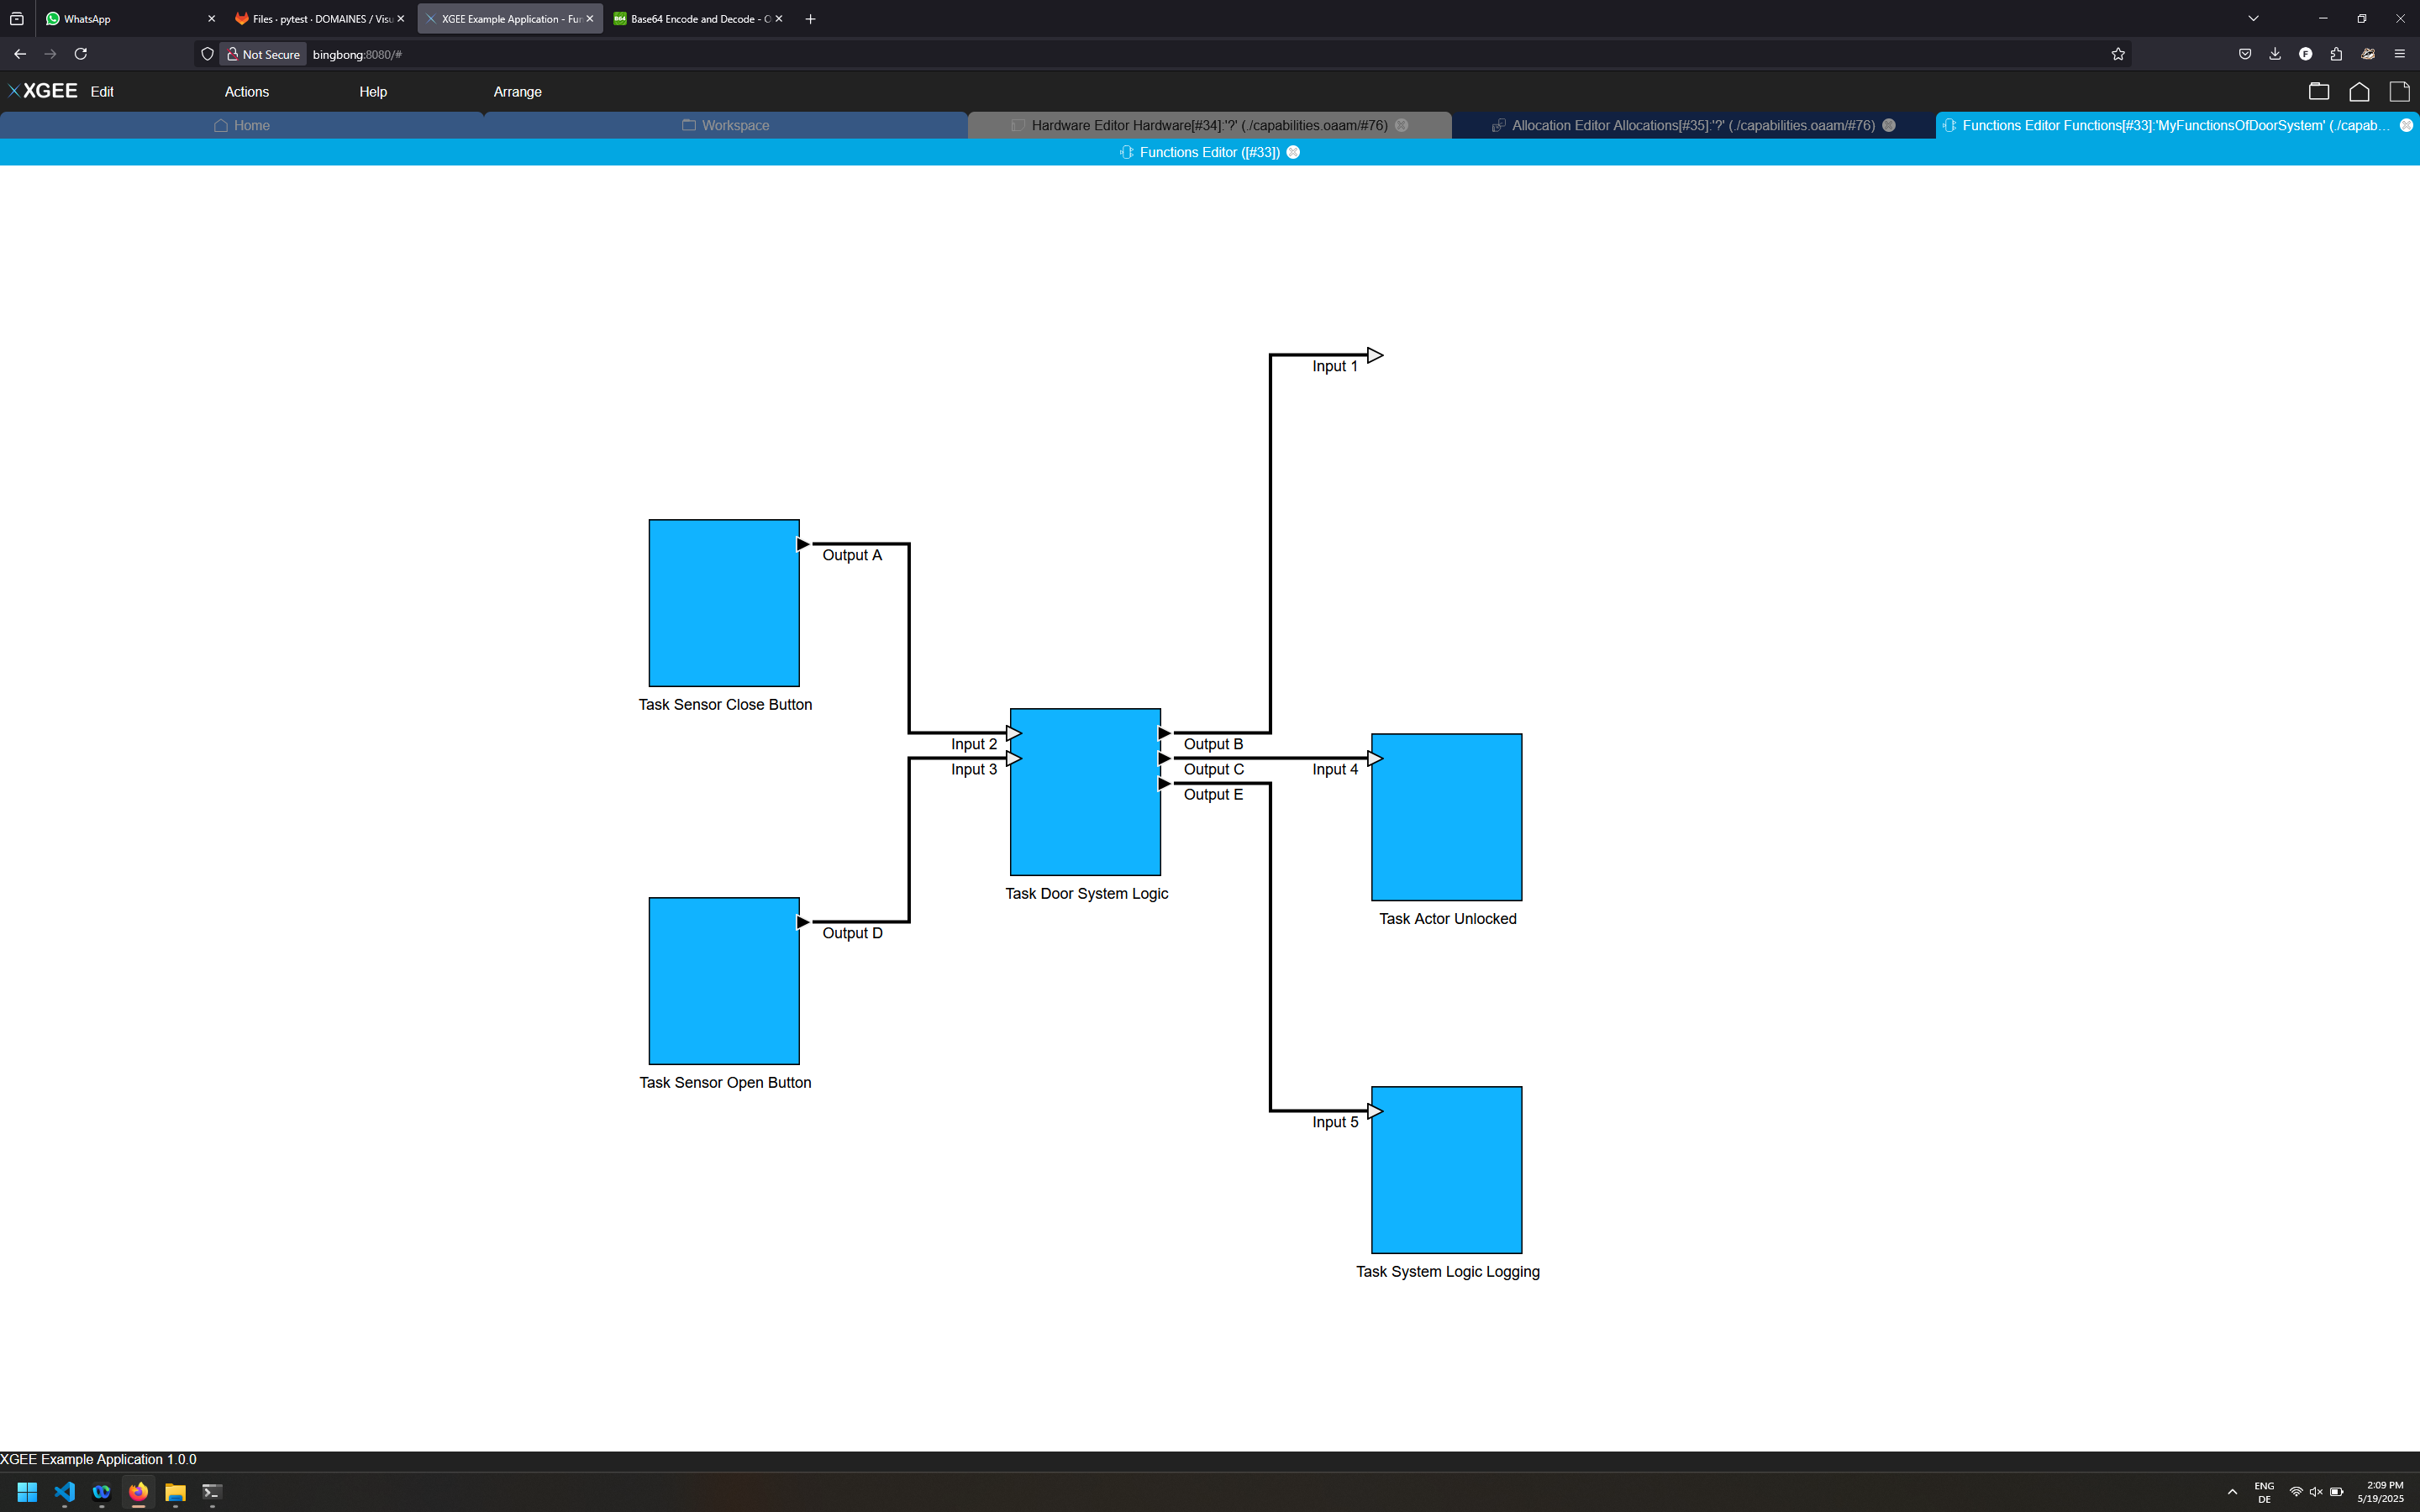
\includegraphics[width=\textwidth]{testcases/vertex_without_parent/140908-928722_input_image.png}
        \caption*{\textit{Before}}
    \end{subfigure}
    \newline
    \begin{subfigure}[t]{0.9\textwidth}
        \centering
        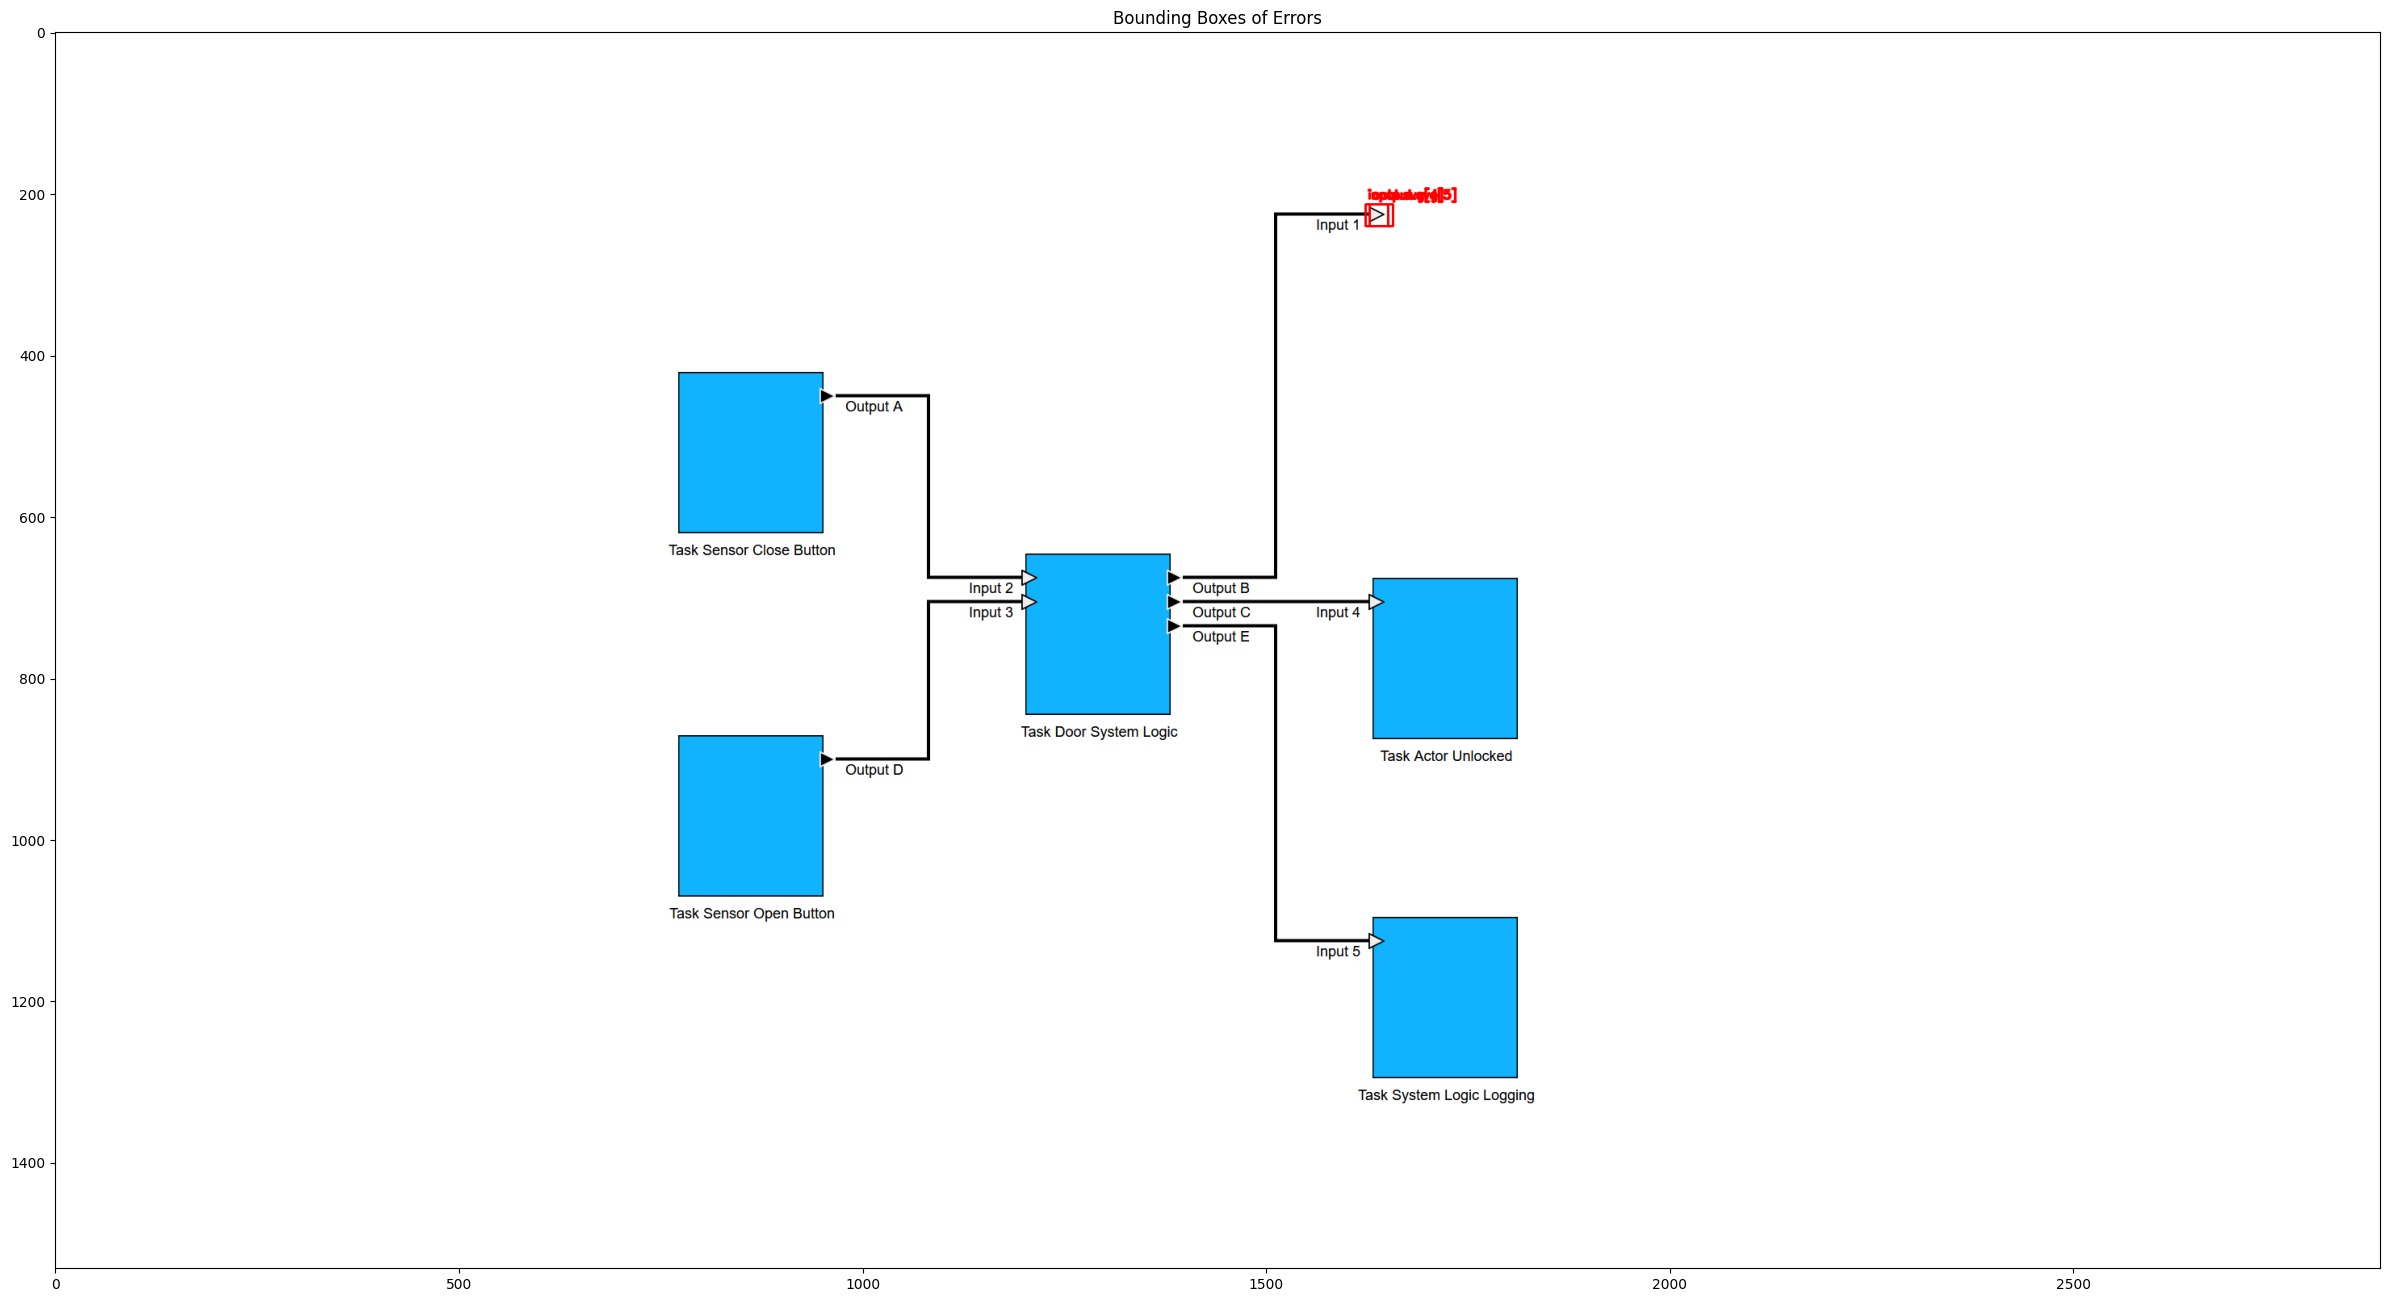
\includegraphics[width=\textwidth]{testcases/vertex_without_parent/140928-590960_element_bbox_errors_labeled_colored.png}
        \caption*{\textit{After}}
    \end{subfigure}
    % \caption{Vertex without parent element}
    \label{fig:vertex_without_parent}
\end{figure}
\newpage

\section{Vertex displayed incorrectly}
\begin{figure}[H]
    \centering
    \begin{subfigure}[t]{0.9\textwidth}
        \centering
        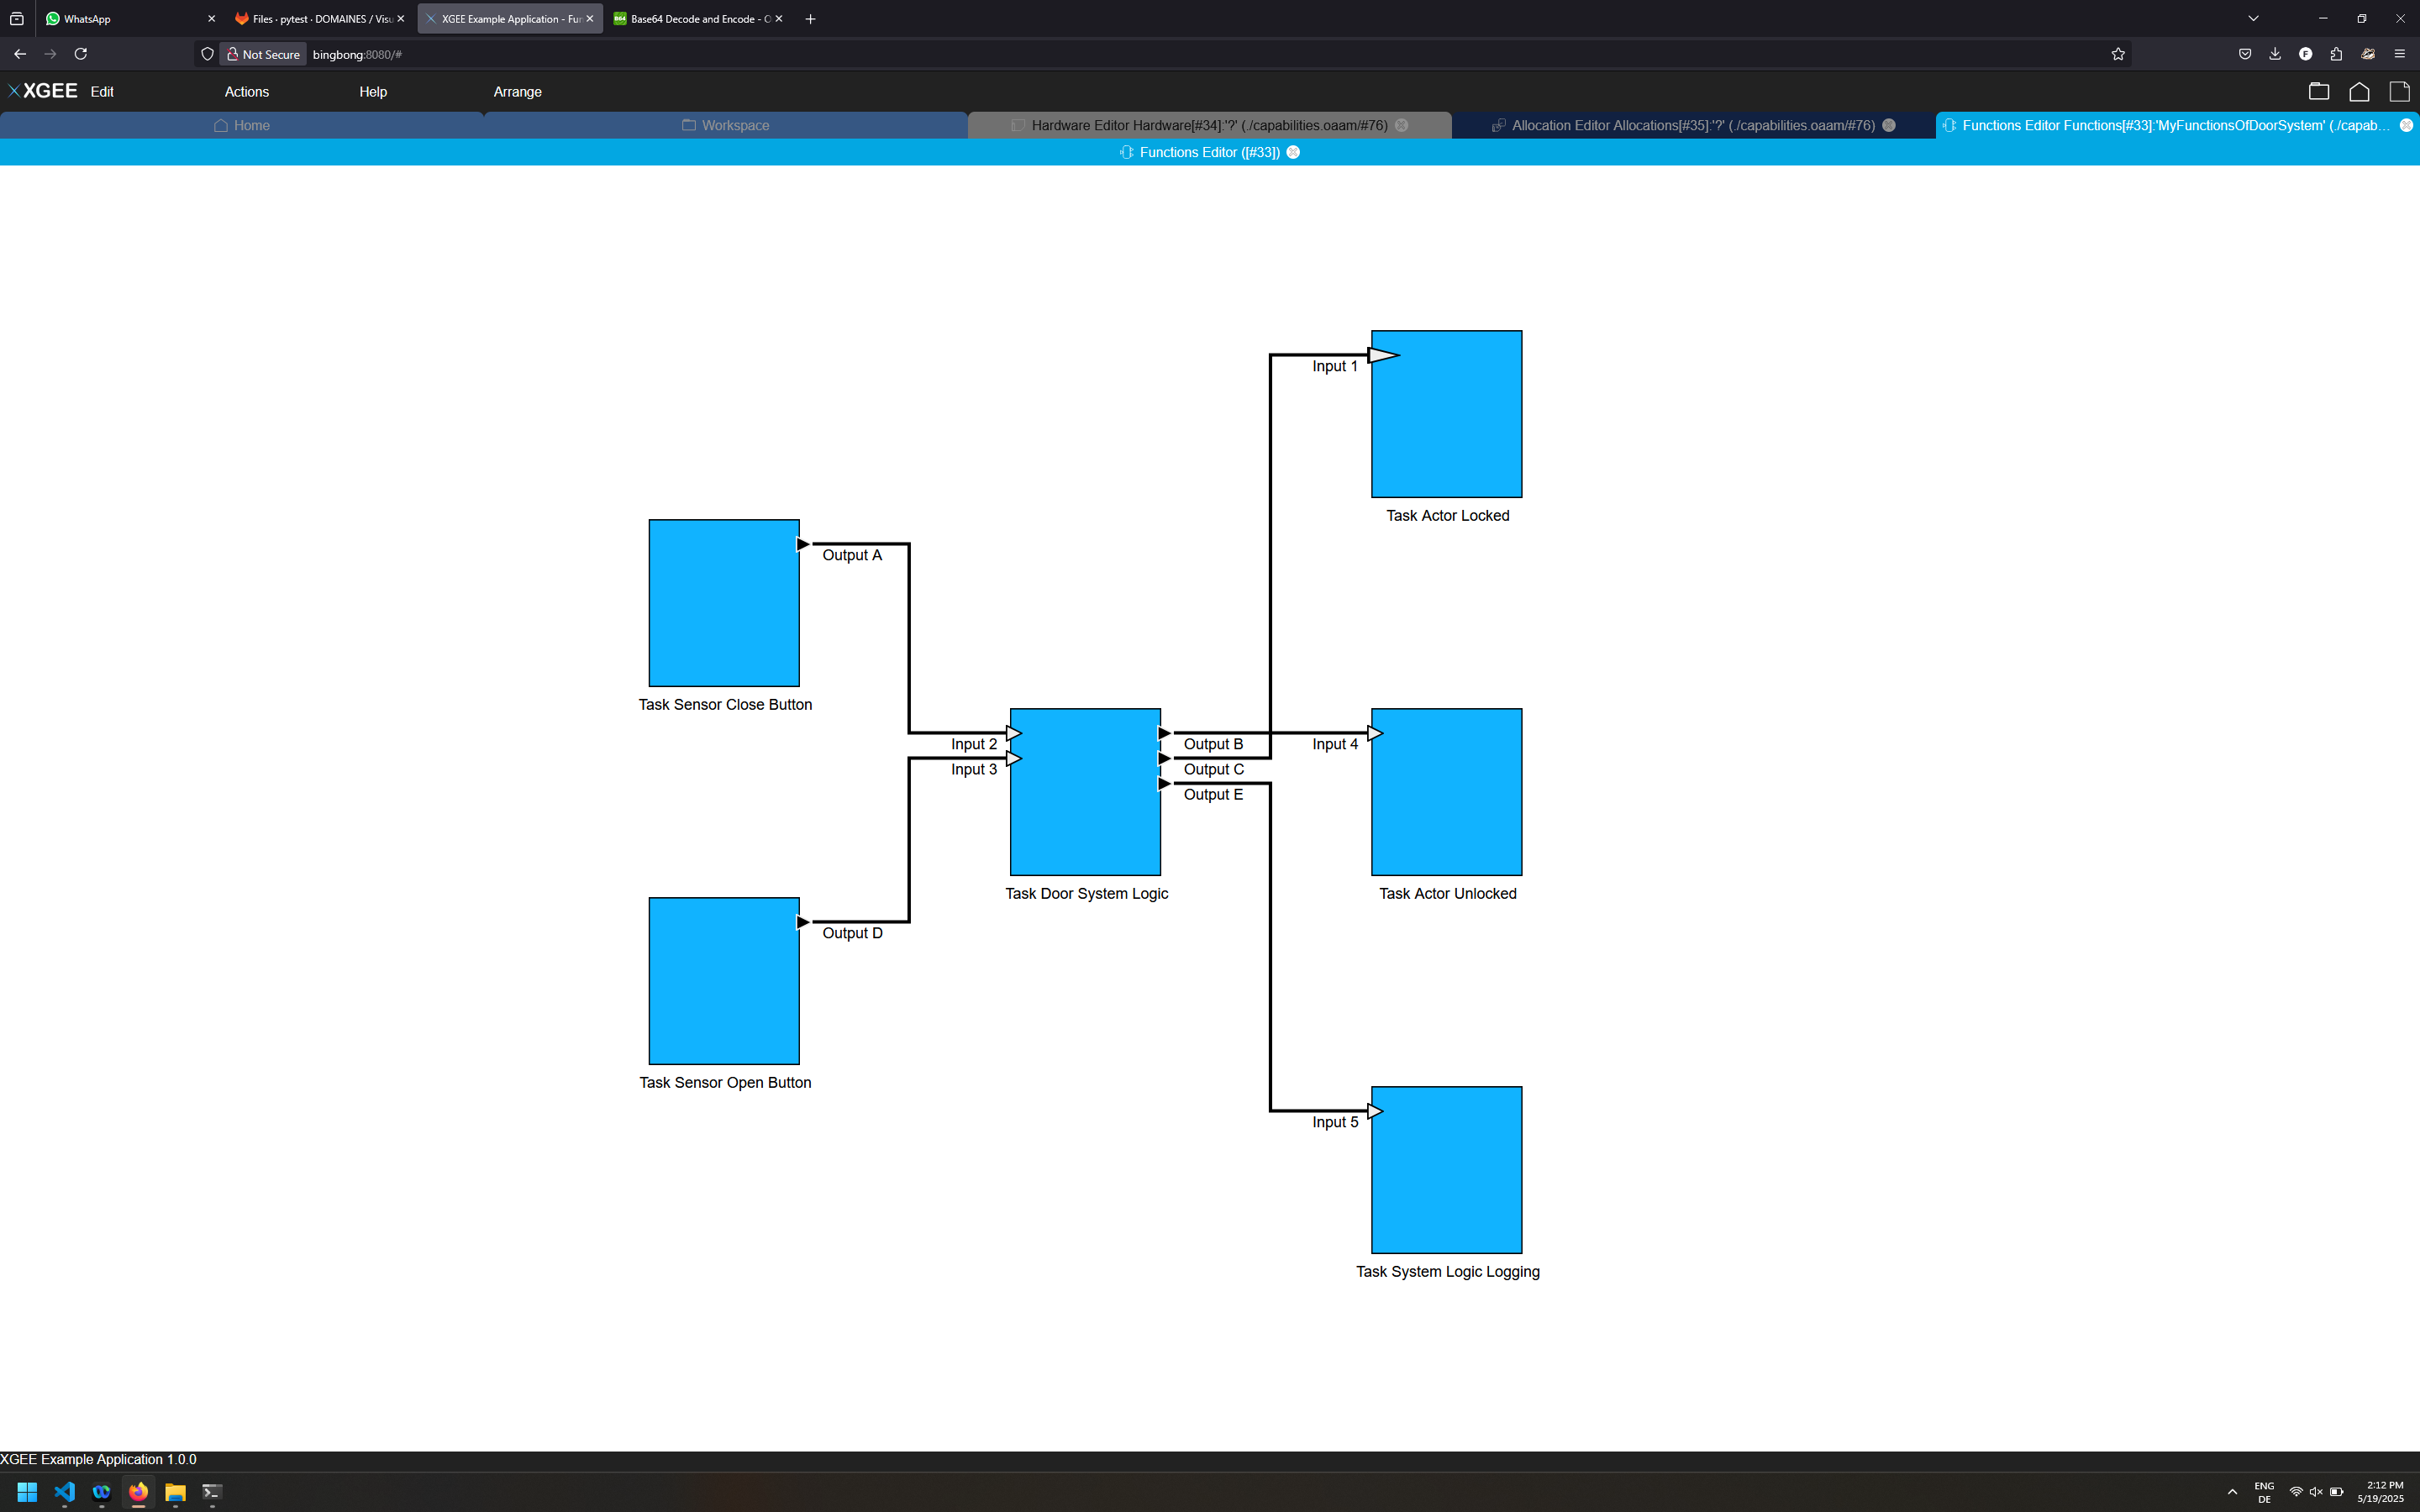
\includegraphics[width=\textwidth]{testcases/vertex_displayed_incorrectly/141215-507428_input_image.png}
        \caption*{\textit{Before}}
    \end{subfigure}
    \newline
    \begin{subfigure}[t]{0.9\textwidth}
        \centering
        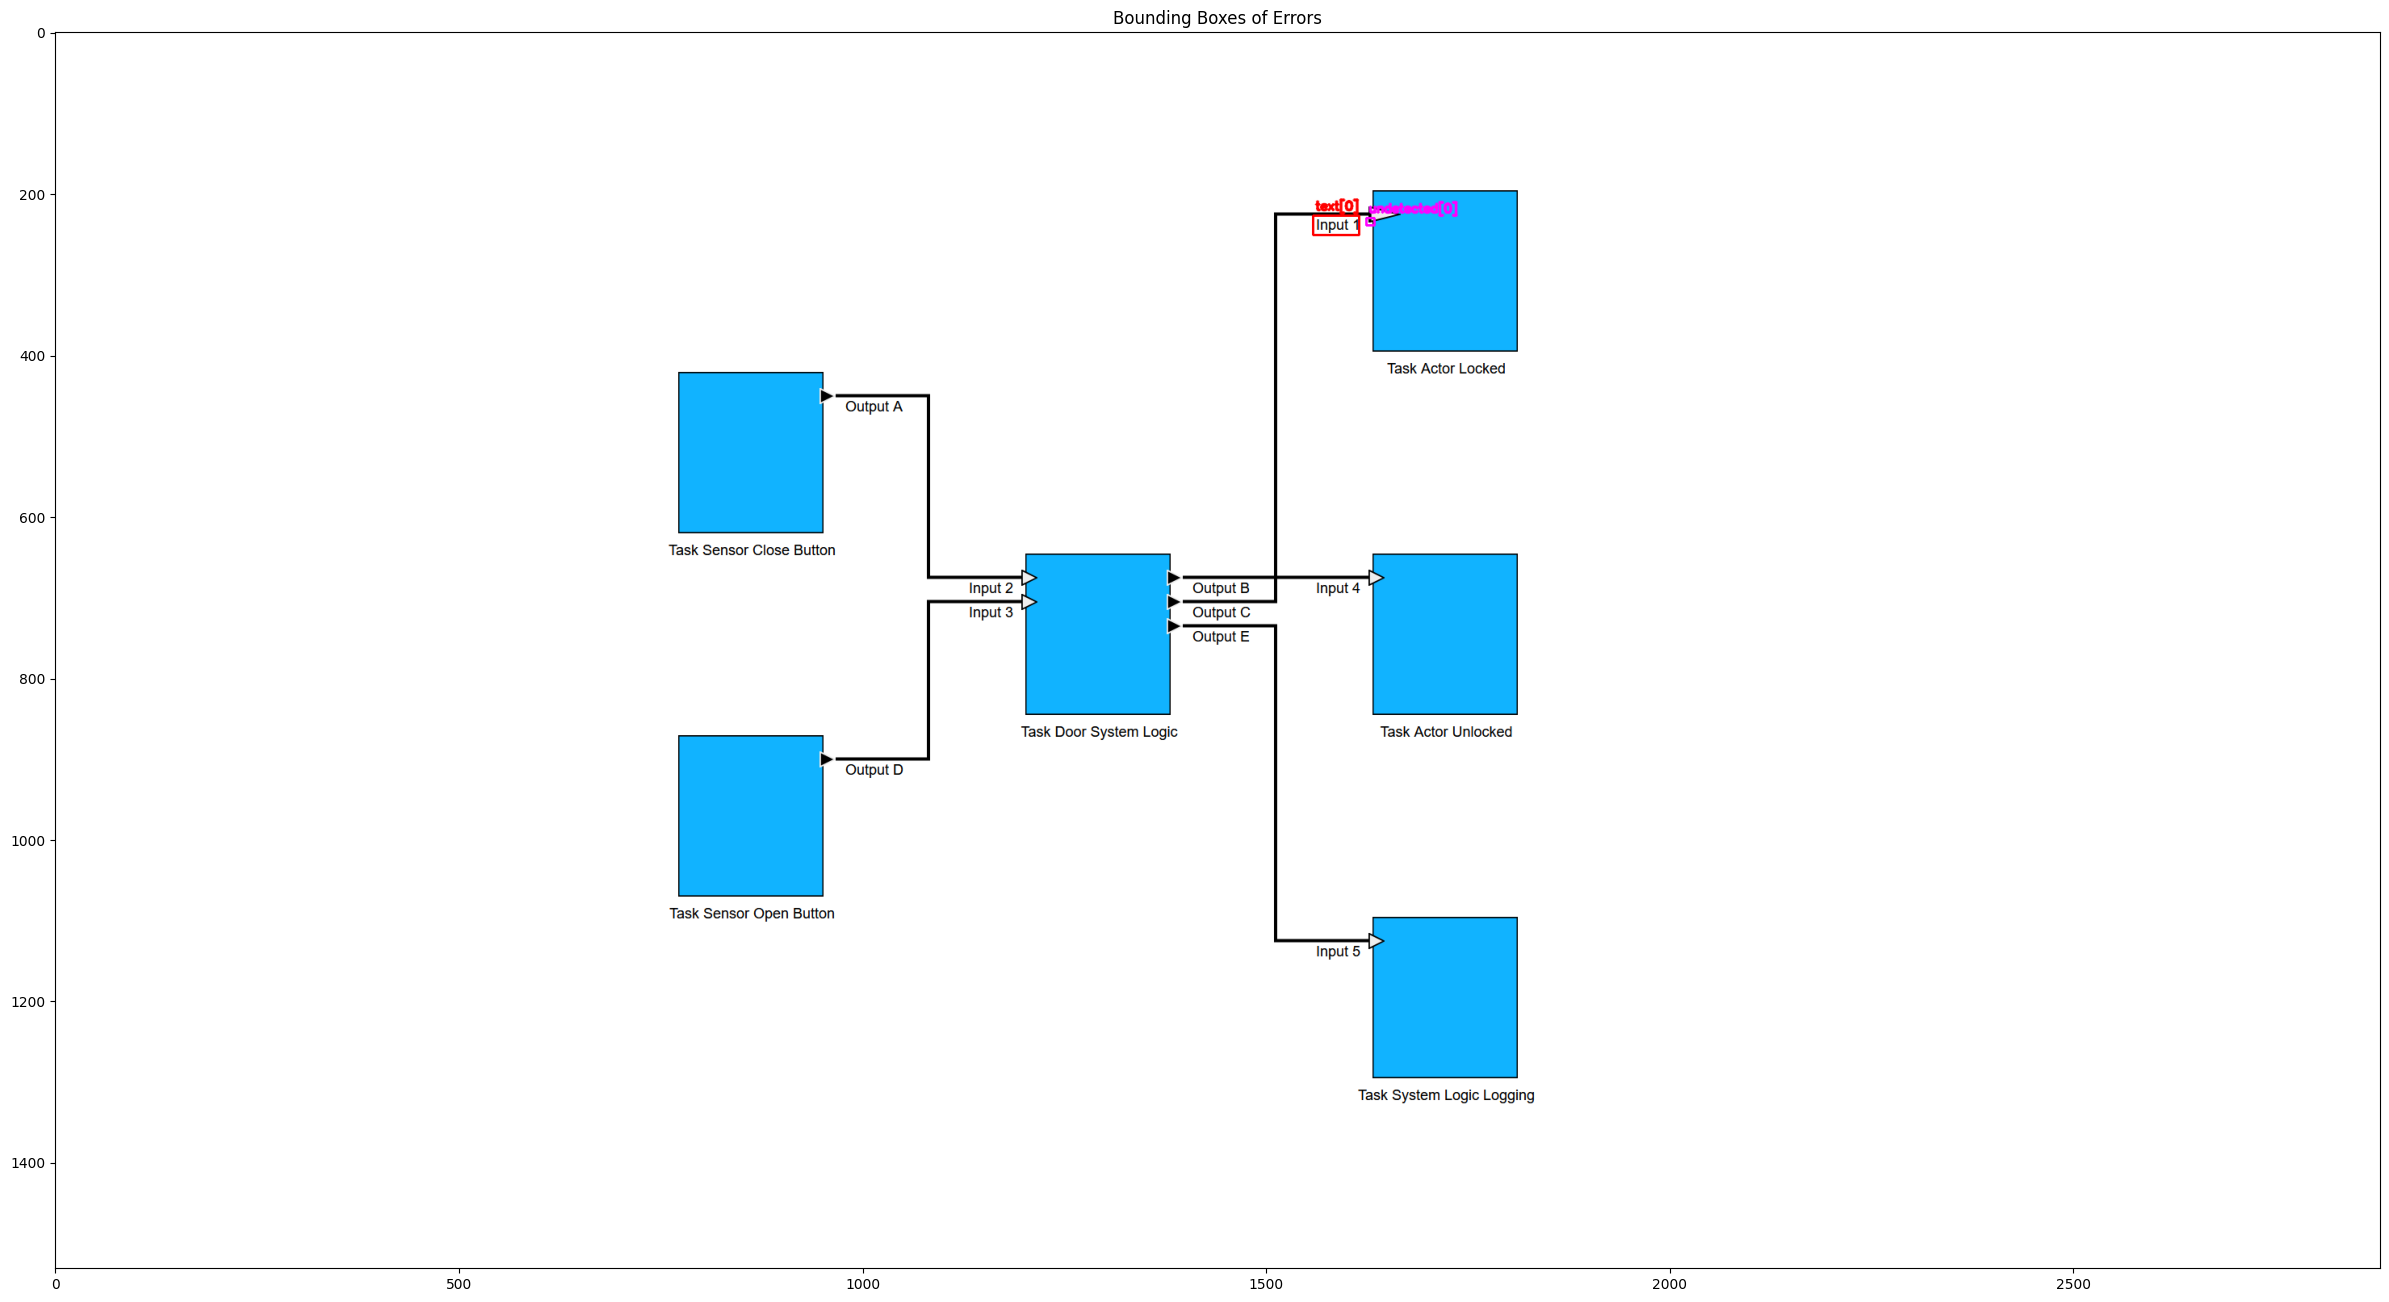
\includegraphics[width=\textwidth]{testcases/vertex_displayed_incorrectly/141236-249257_element_bbox_errors_labeled_colored.png}
        \caption*{\textit{After}}
    \end{subfigure}
    % \caption{Vertex displayed incorrectly}
    \label{fig:vertex_displayed_incorrectly}
\end{figure}
\newpage

\section{Vertex in visualization, but not in model}

\newpage

\section{Vertex in model, but not in visualization}
\begin{figure}[H]
    \centering
    \begin{subfigure}[t]{0.9\textwidth}
        \centering
        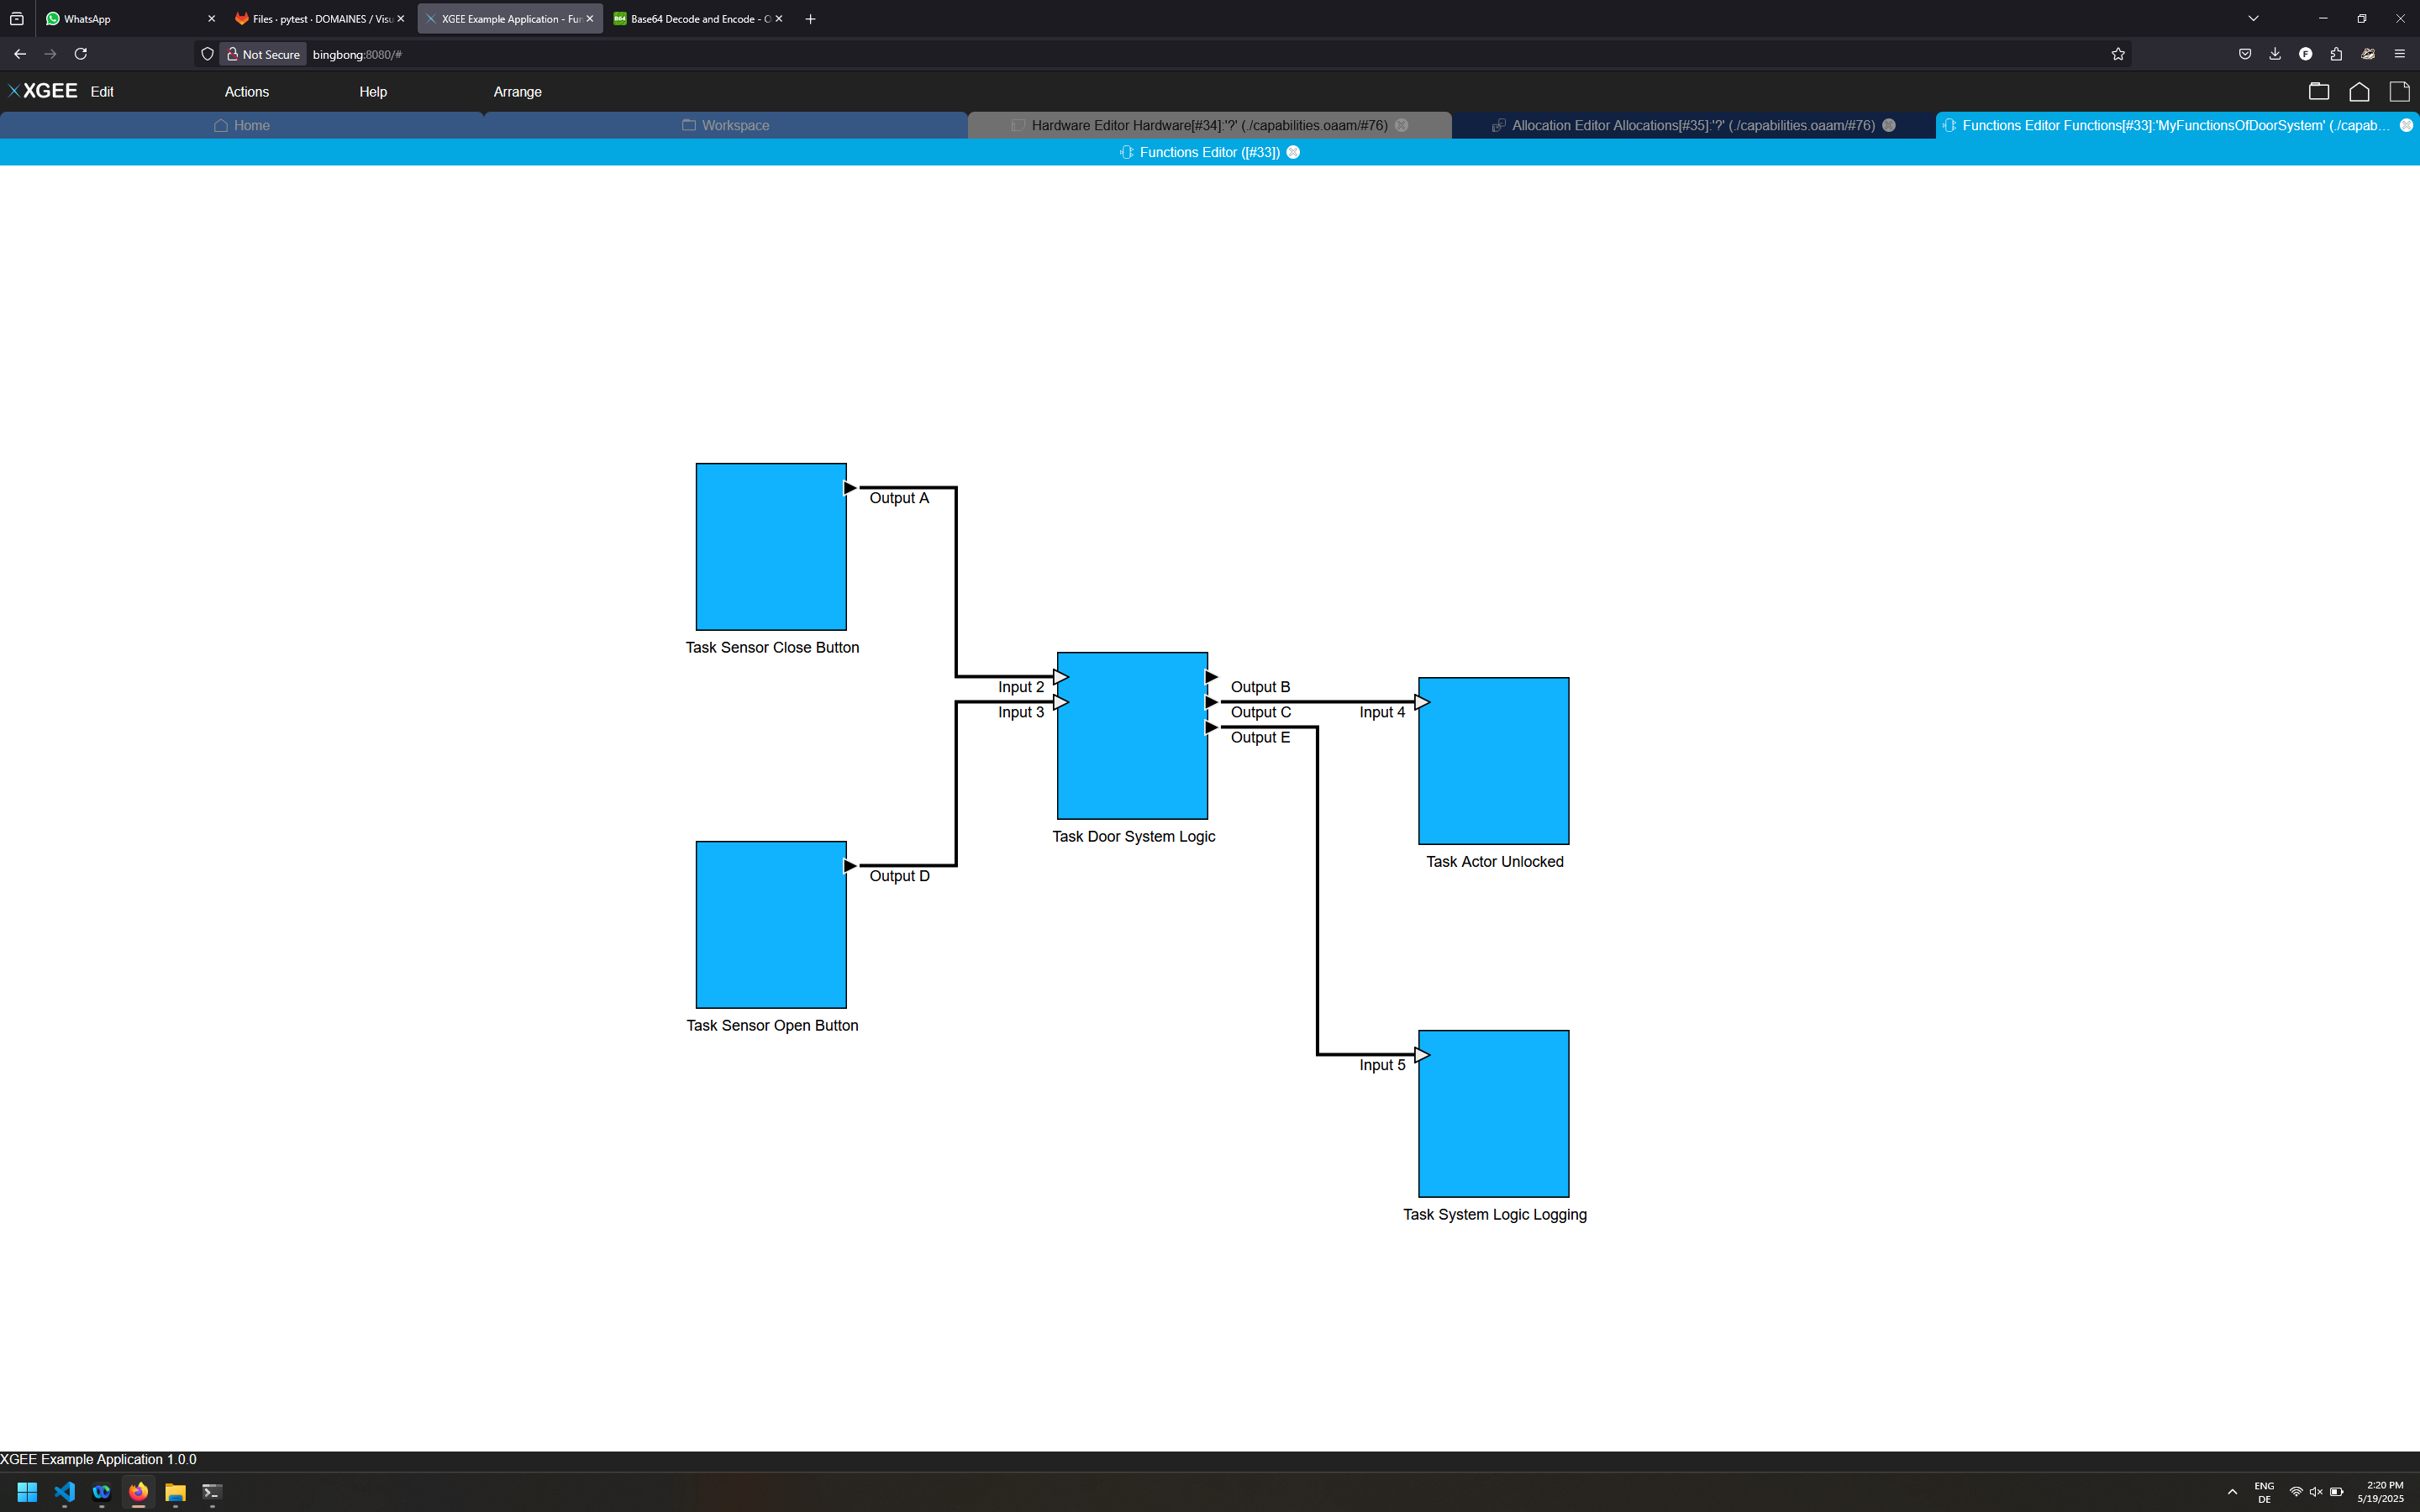
\includegraphics[width=\textwidth]{testcases/vertex_in_model_not_in_visualization/142027-594237_input_image.png}
        \caption*{\textit{Before}}
    \end{subfigure}
    \newline
    \begin{subfigure}[t]{0.9\textwidth}
        \centering
        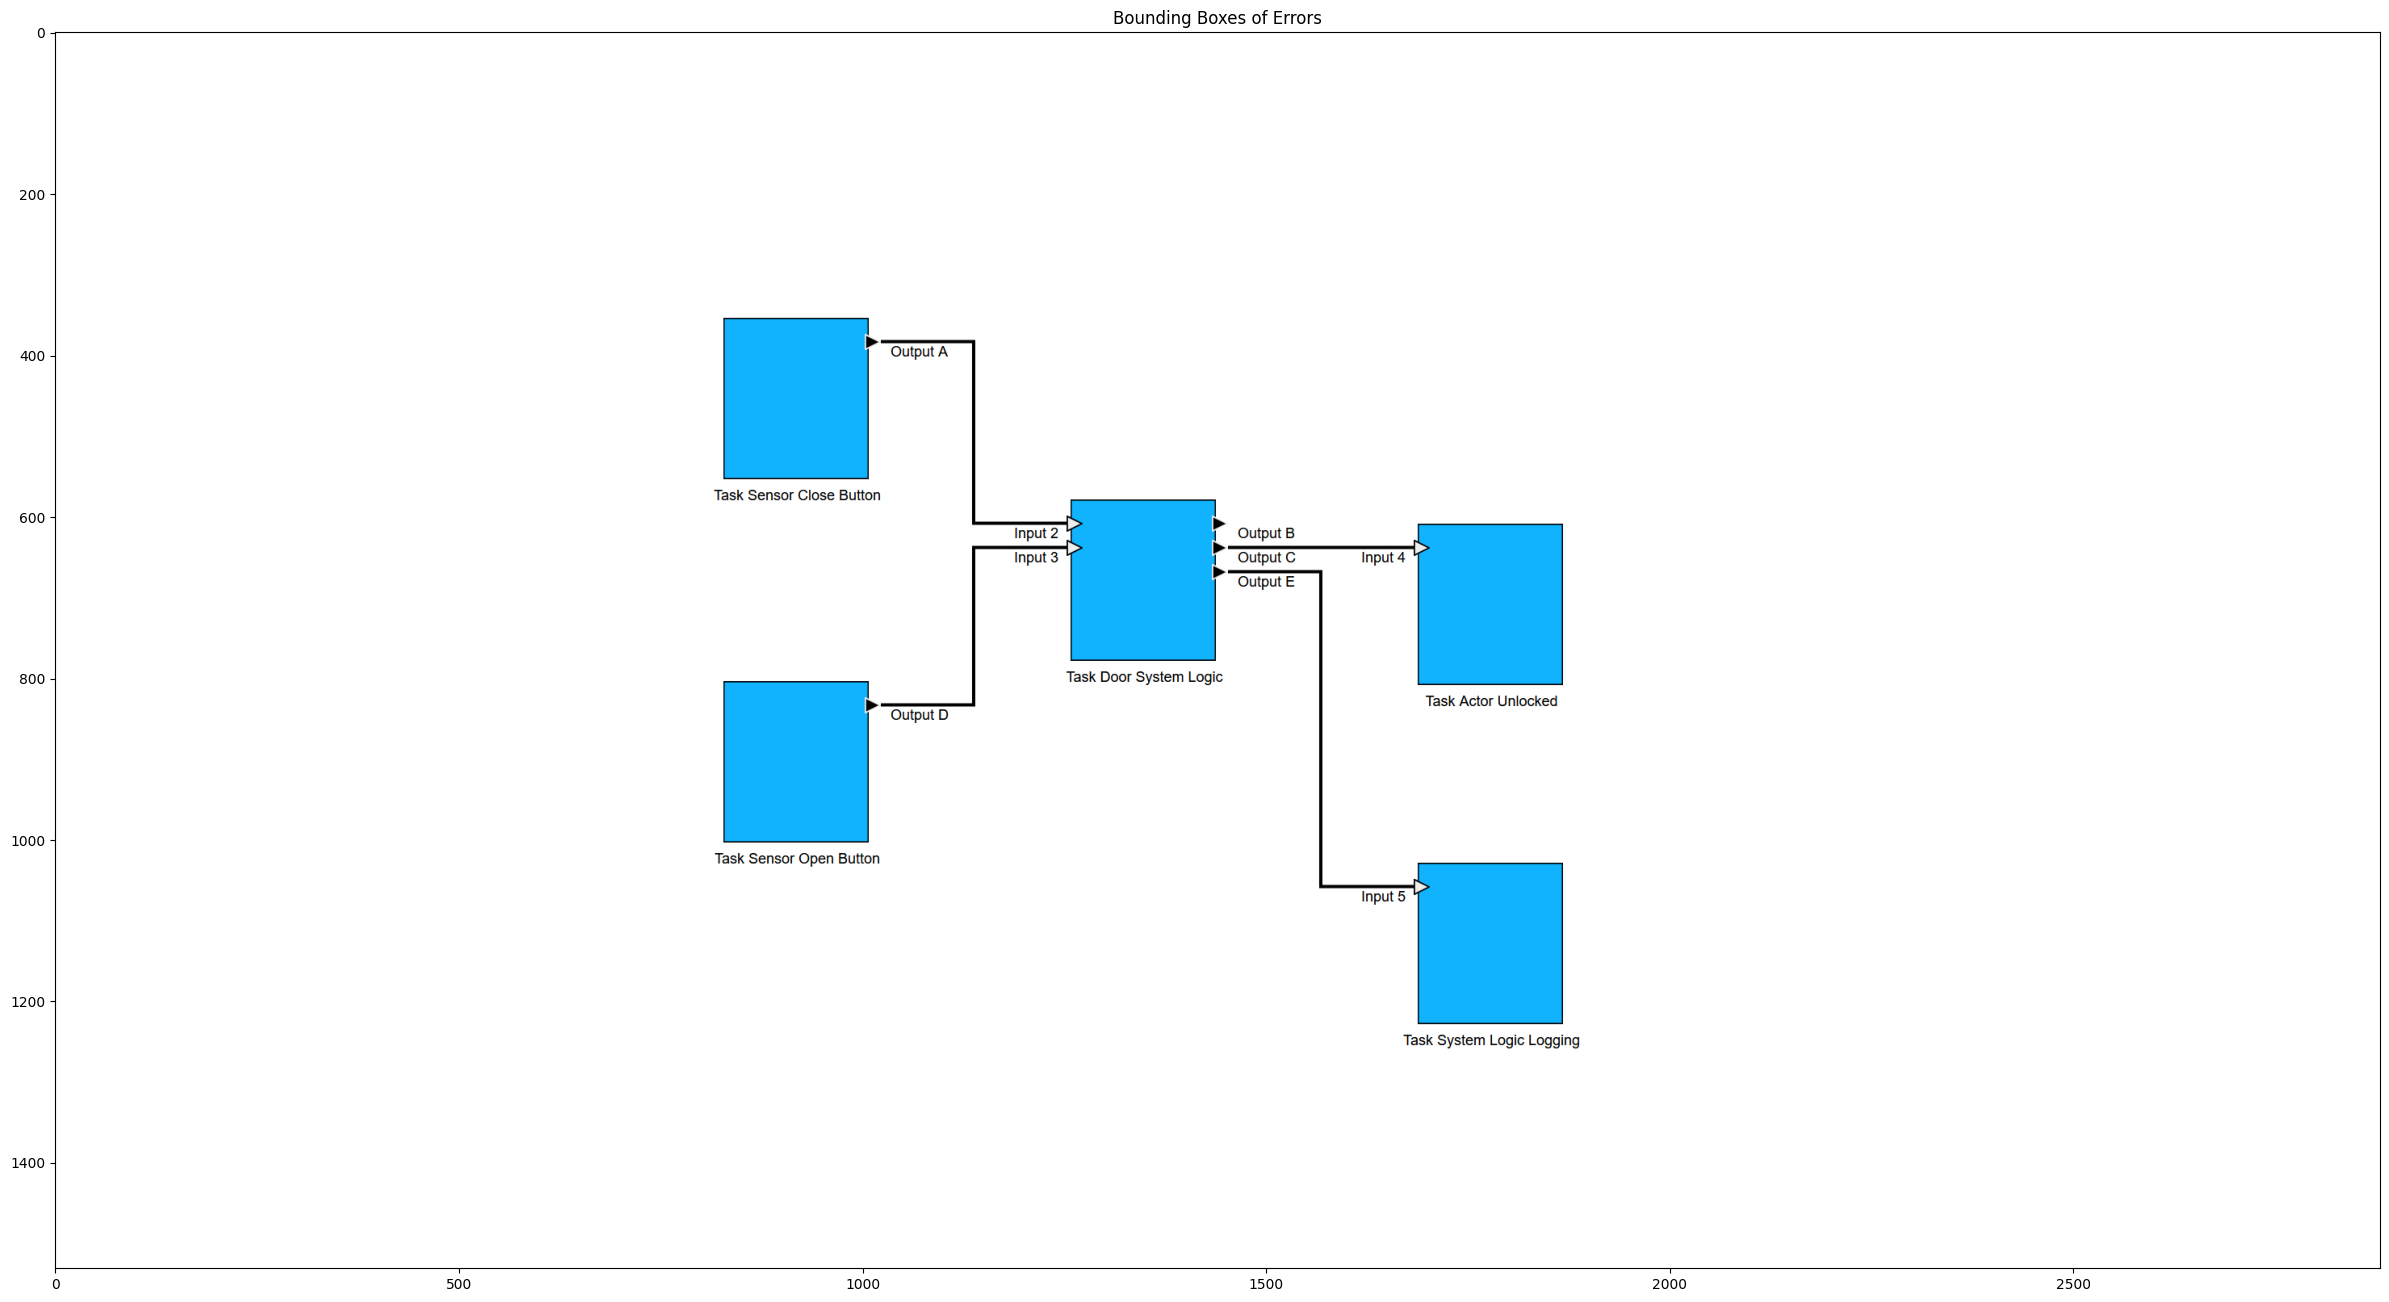
\includegraphics[width=\textwidth]{testcases/vertex_in_model_not_in_visualization/142047-652879_element_bbox_errors_labeled_colored.png}
        \caption*{\textit{After}}
    \end{subfigure}
    % \caption{Vertex in model, but not in visualization}
    \label{fig:vertex_in_model_not_viz}
\end{figure}
\newpage

% ------------------------
% Edge Issues
% ------------------------

\section{Edge too thin}
\begin{figure}[H]
    \centering
    \begin{subfigure}[t]{0.9\textwidth}
        \centering
        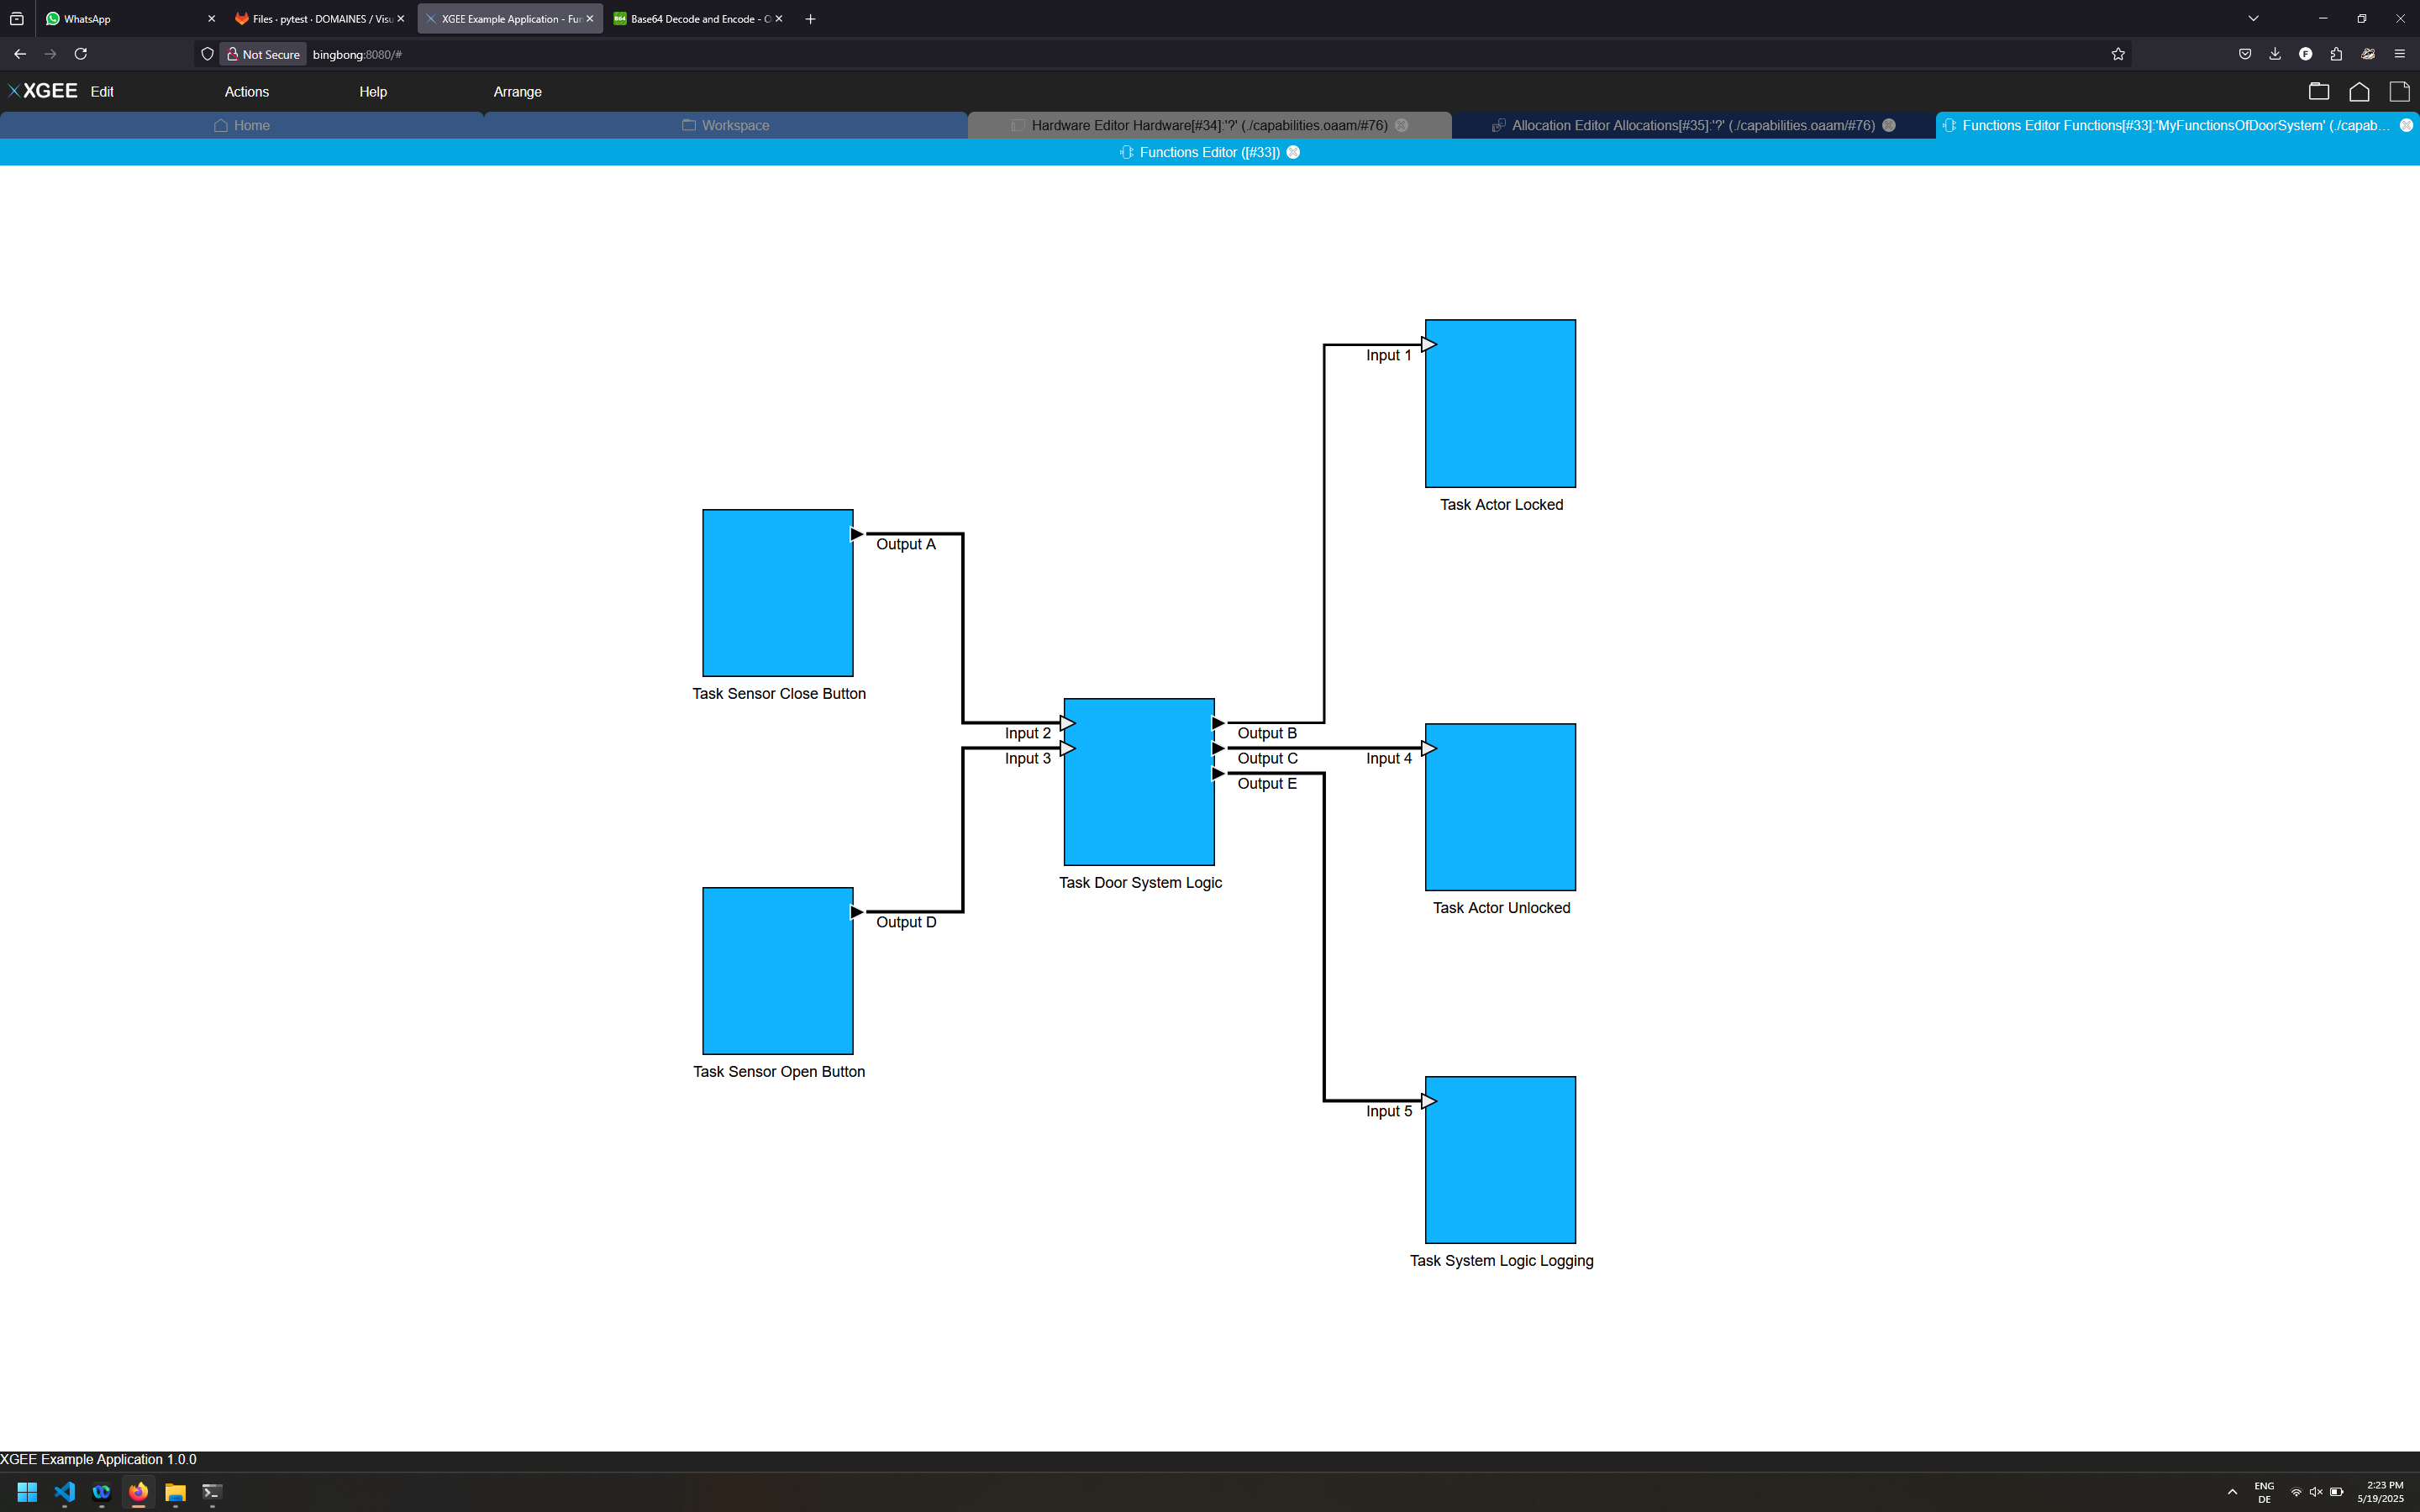
\includegraphics[width=\textwidth]{testcases/edge_1px_too_thin/142331-026220_input_image.png}
        \caption*{\textit{Before}}
    \end{subfigure}
    \newline    
    \begin{subfigure}[t]{0.9\textwidth}
        \centering
        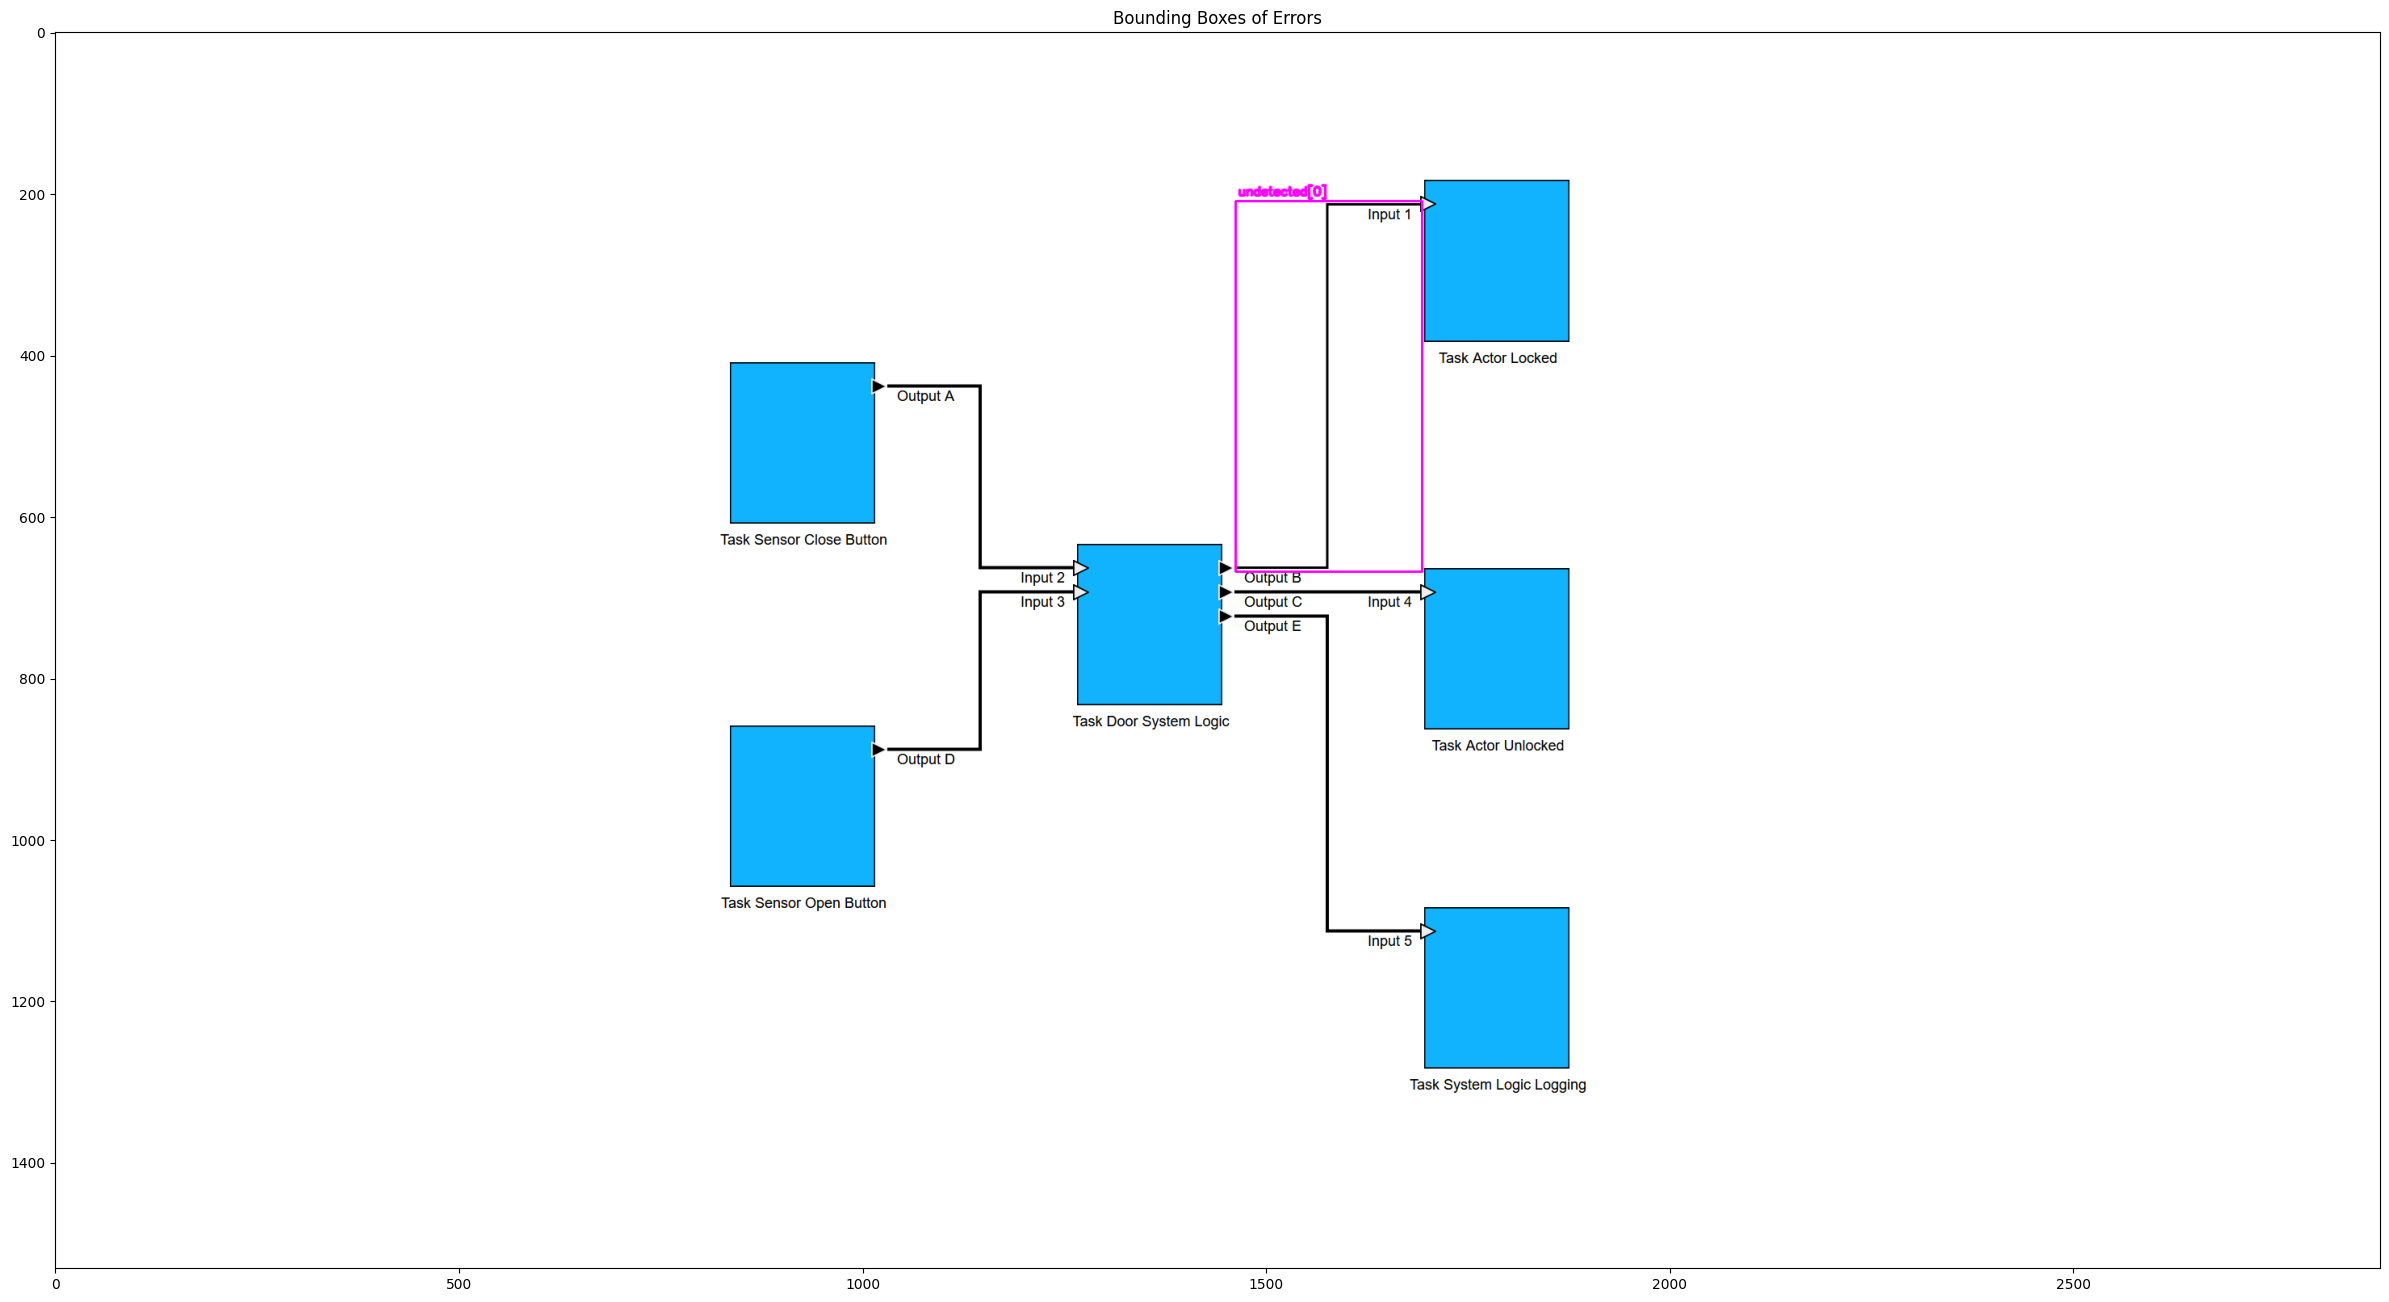
\includegraphics[width=\textwidth]{testcases/edge_1px_too_thin/142351-849844_element_bbox_errors_labeled_colored.png}
        \caption*{\textit{After}}
    \end{subfigure}
    % \caption{Edge too thin}
    \label{fig:edge_too_thin}
\end{figure}
\newpage

\section{Edge 1px too wide}
\begin{figure}[H]
    \centering
    \begin{subfigure}[t]{0.9\textwidth}
        \centering
        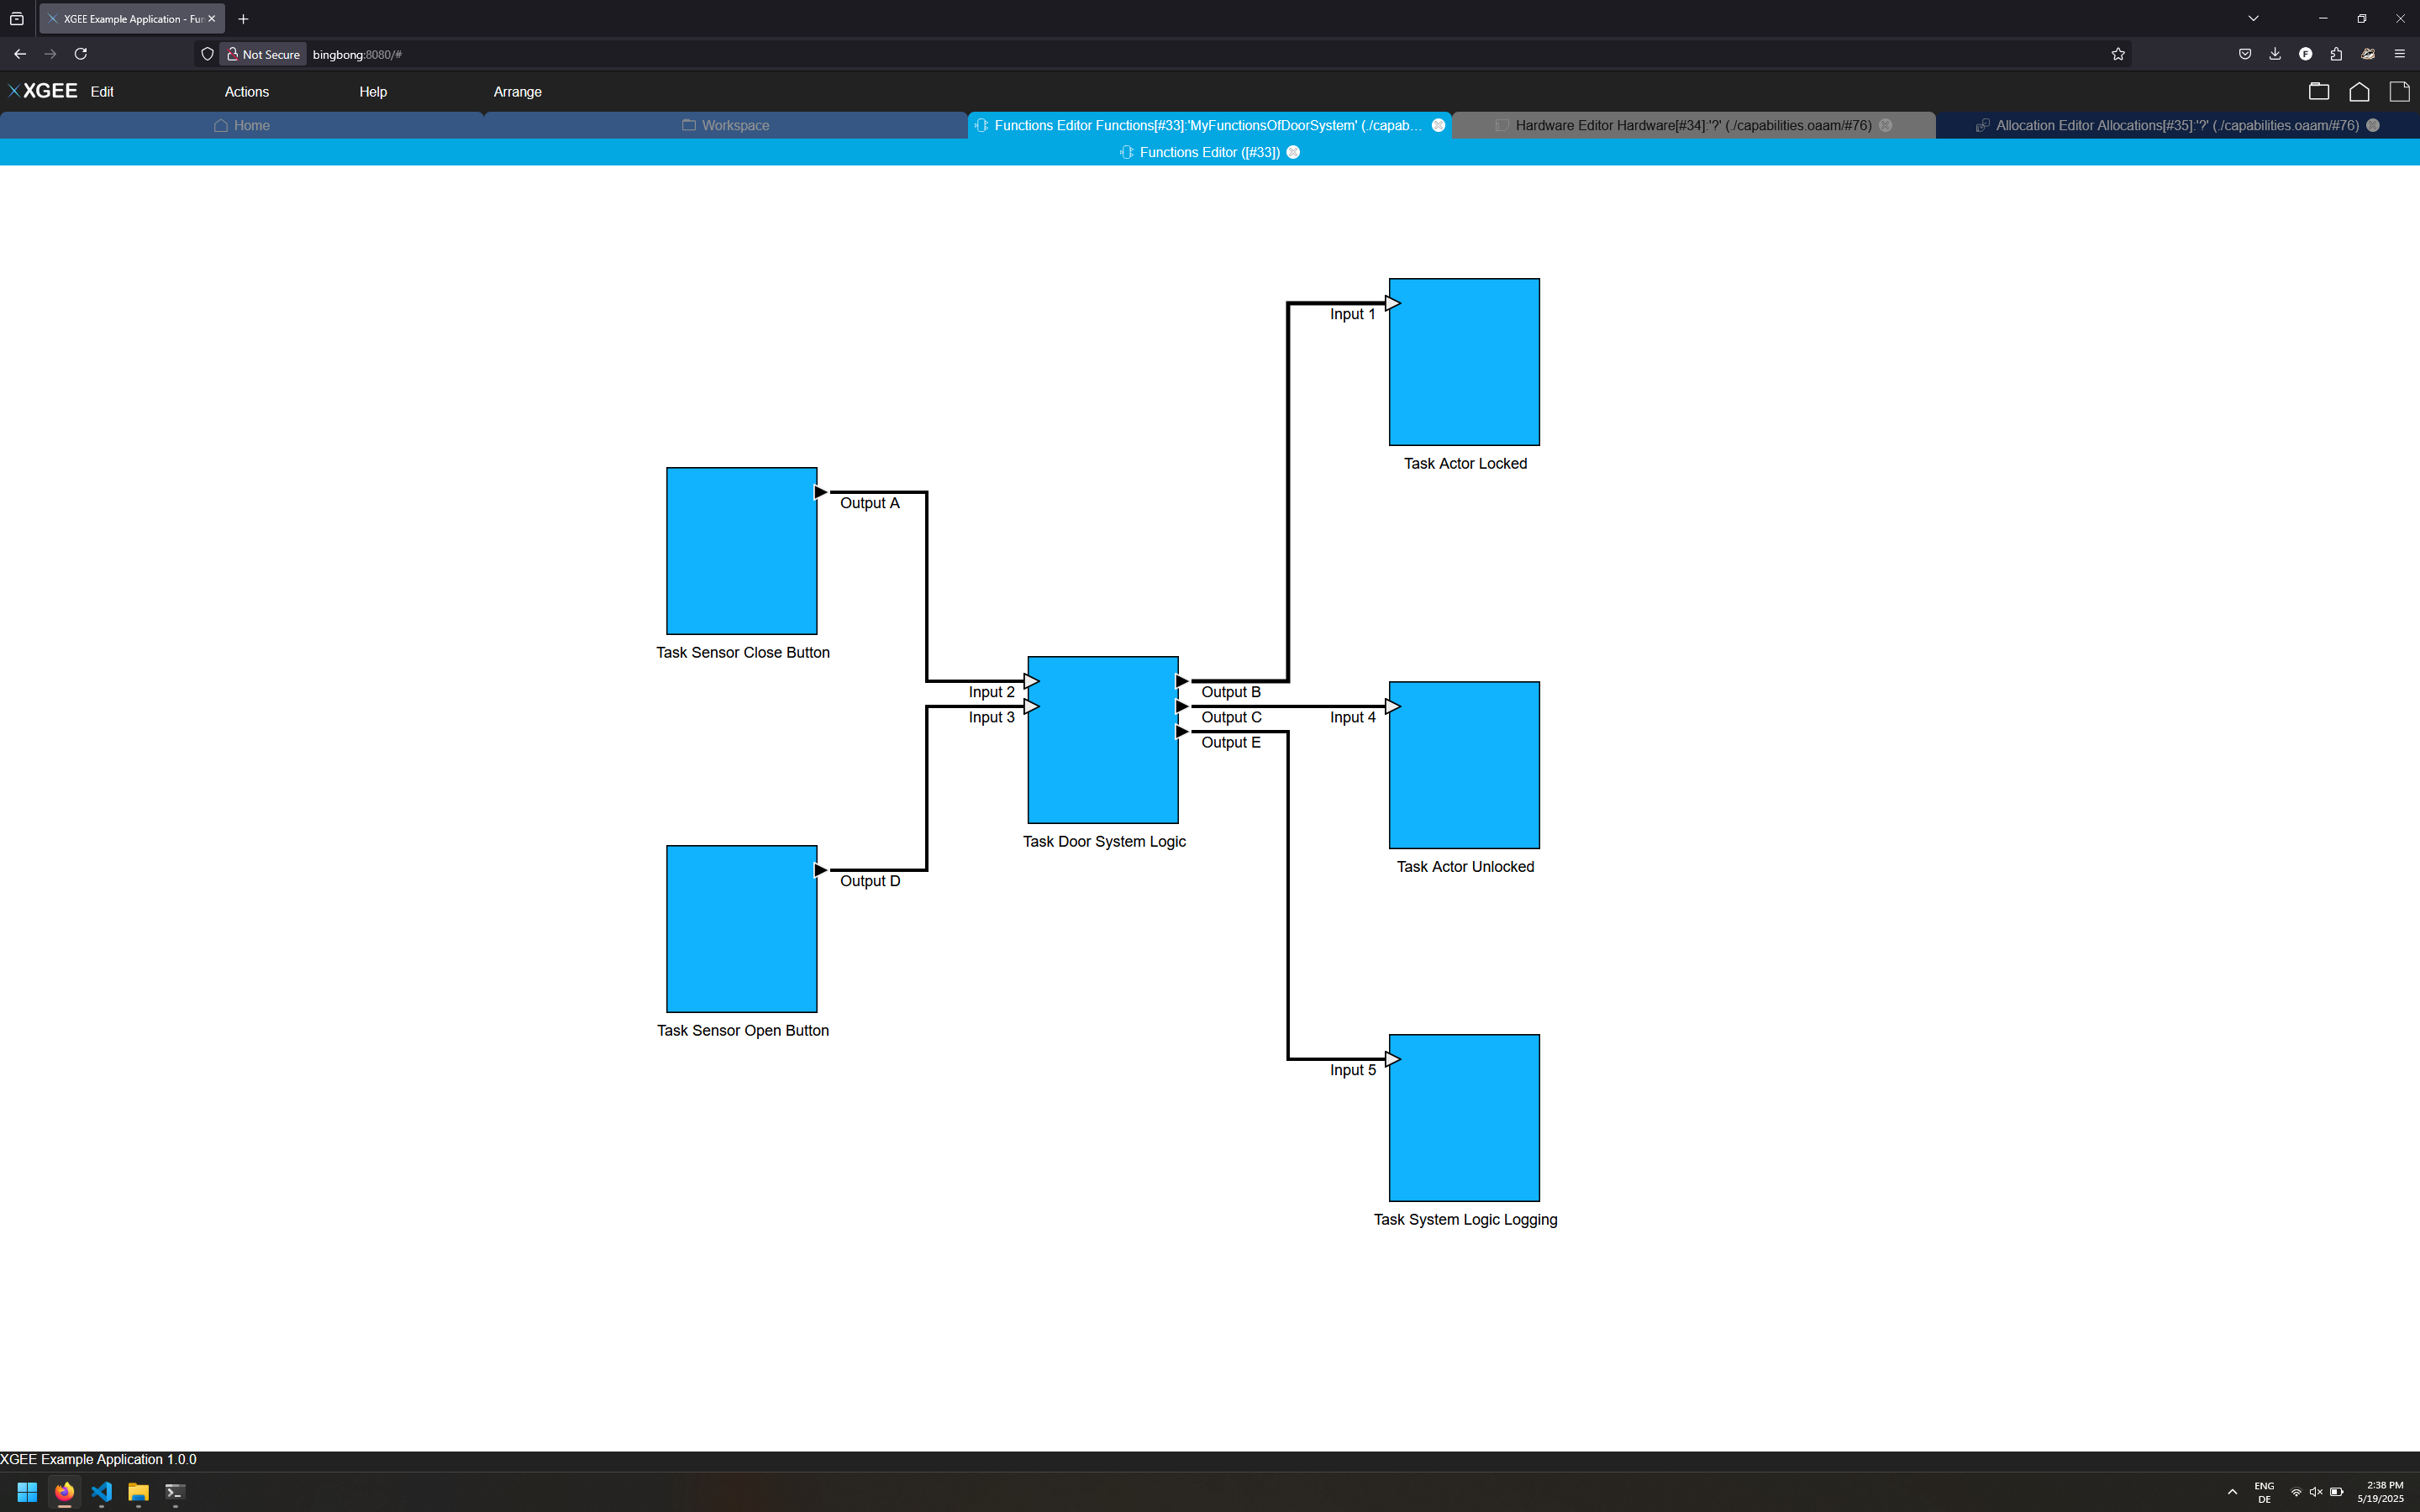
\includegraphics[width=\textwidth]{testcases/edge_1px_too_wide/143815-341162_input_image.png}
        \caption*{\textit{Before}}
    \end{subfigure}
    \newline    
    \begin{subfigure}[t]{0.9\textwidth}
        \centering
        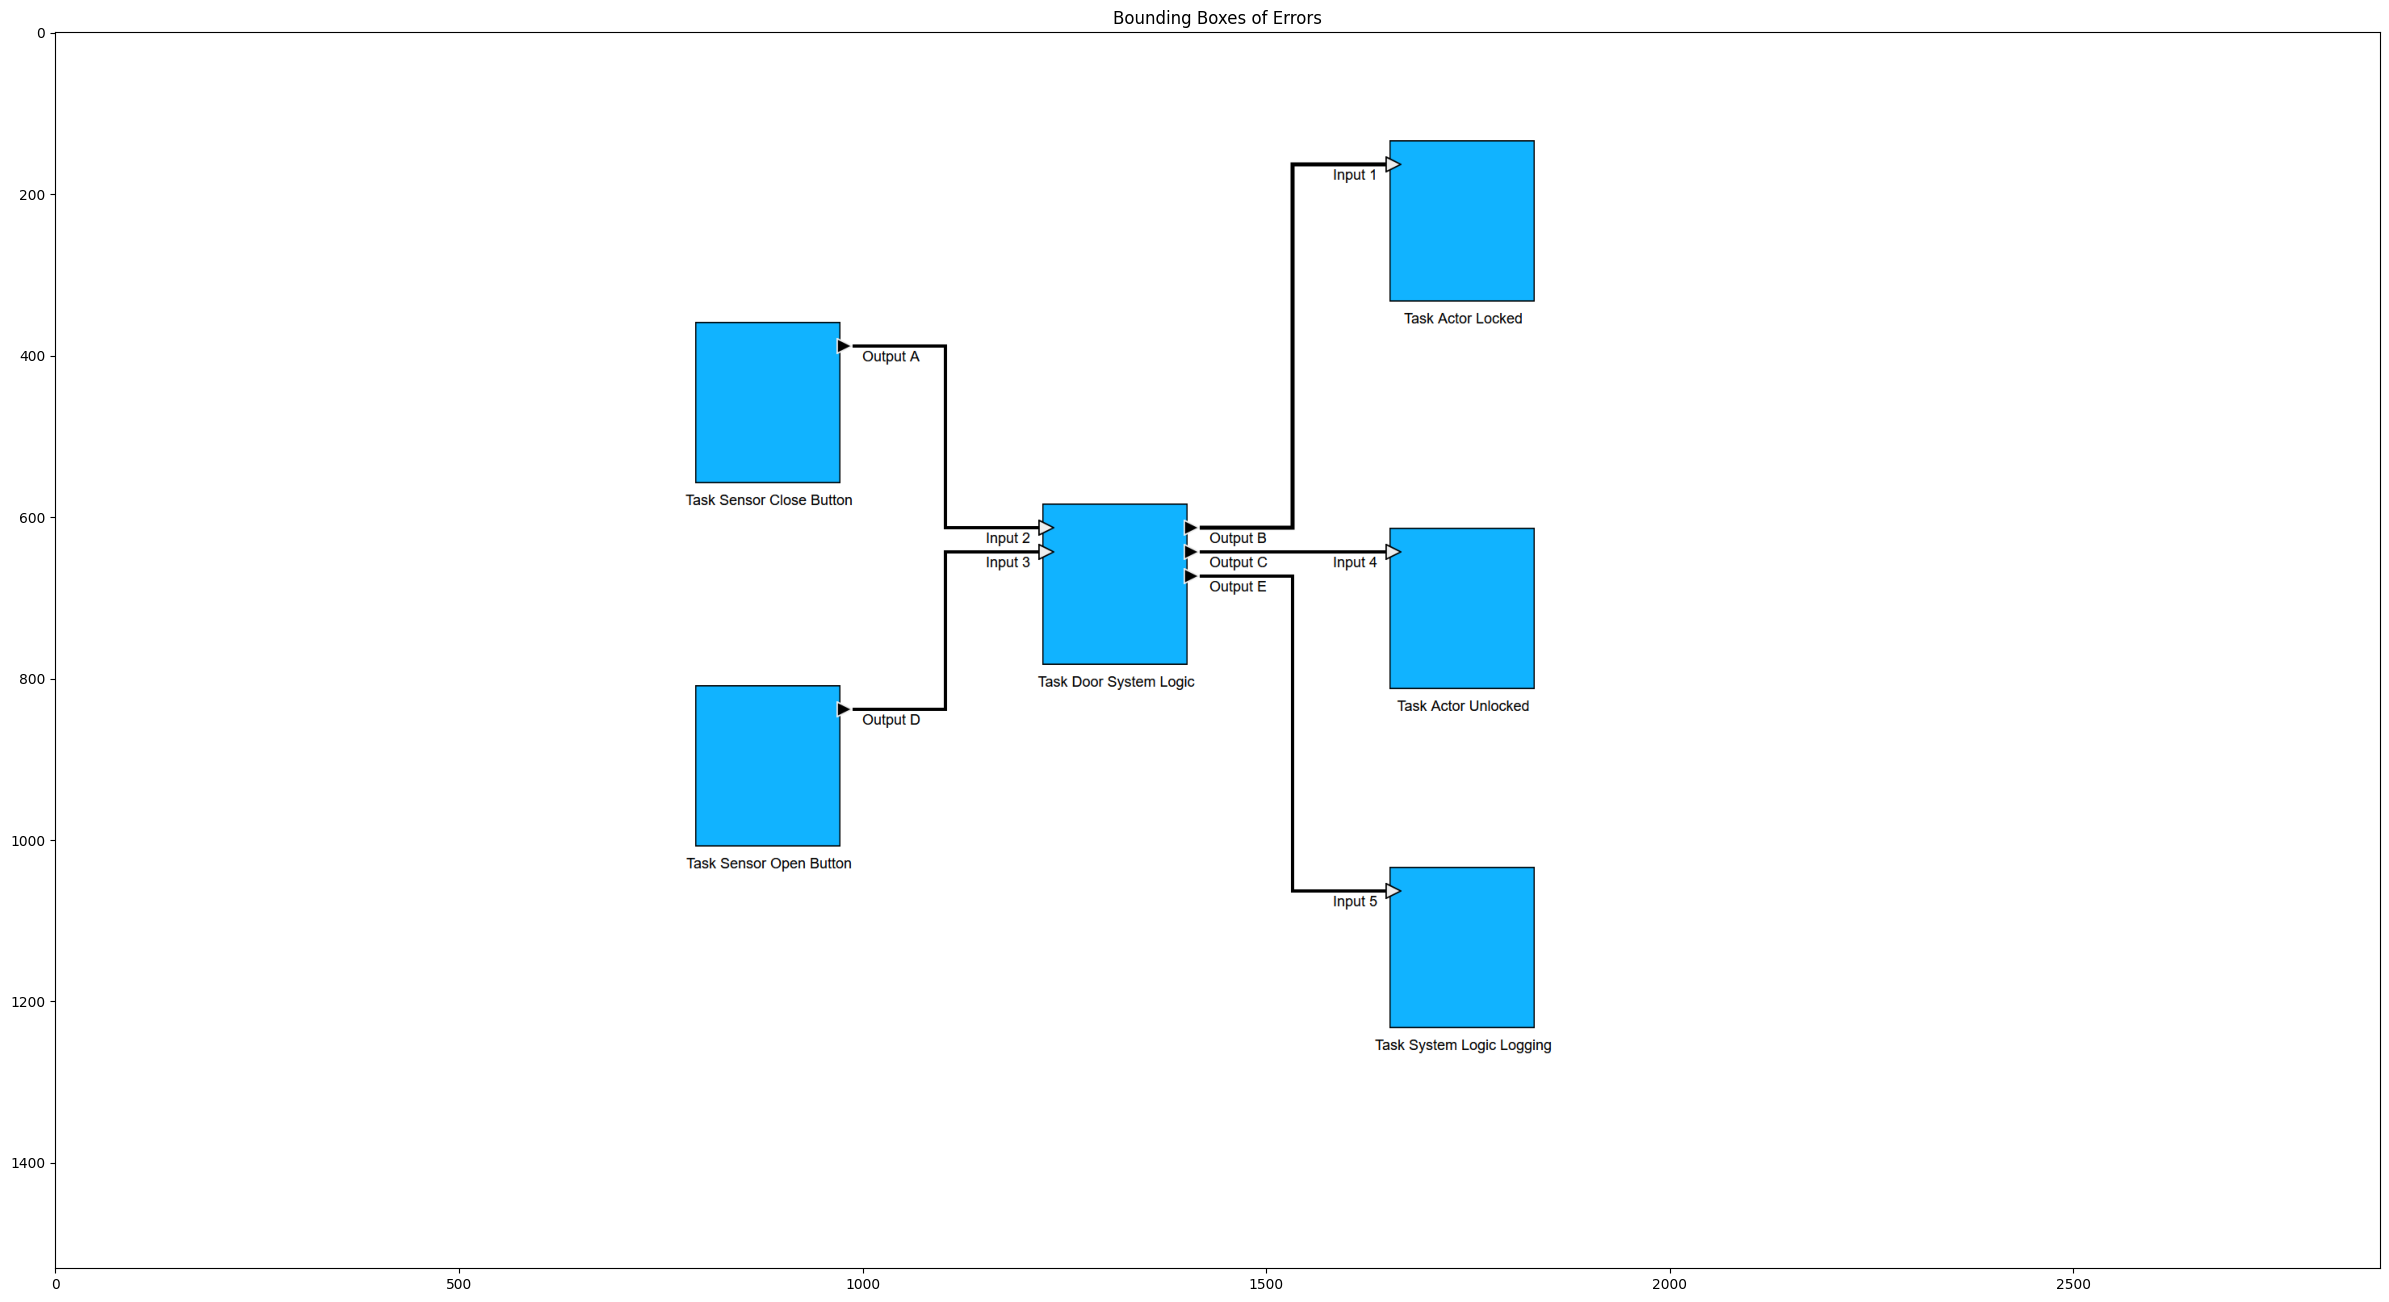
\includegraphics[width=\textwidth]{testcases/edge_1px_too_wide/143838-662391_element_bbox_errors_labeled_colored.png}
        \caption*{\textit{After}}
    \end{subfigure}
    % \caption{Edge too wide}
    \label{fig:edge_too_wide_1}
\end{figure}
\newpage

\section{Edge 2px too wide}
\begin{figure}[H]
    \centering
    \begin{subfigure}[t]{0.9\textwidth}
        \centering
        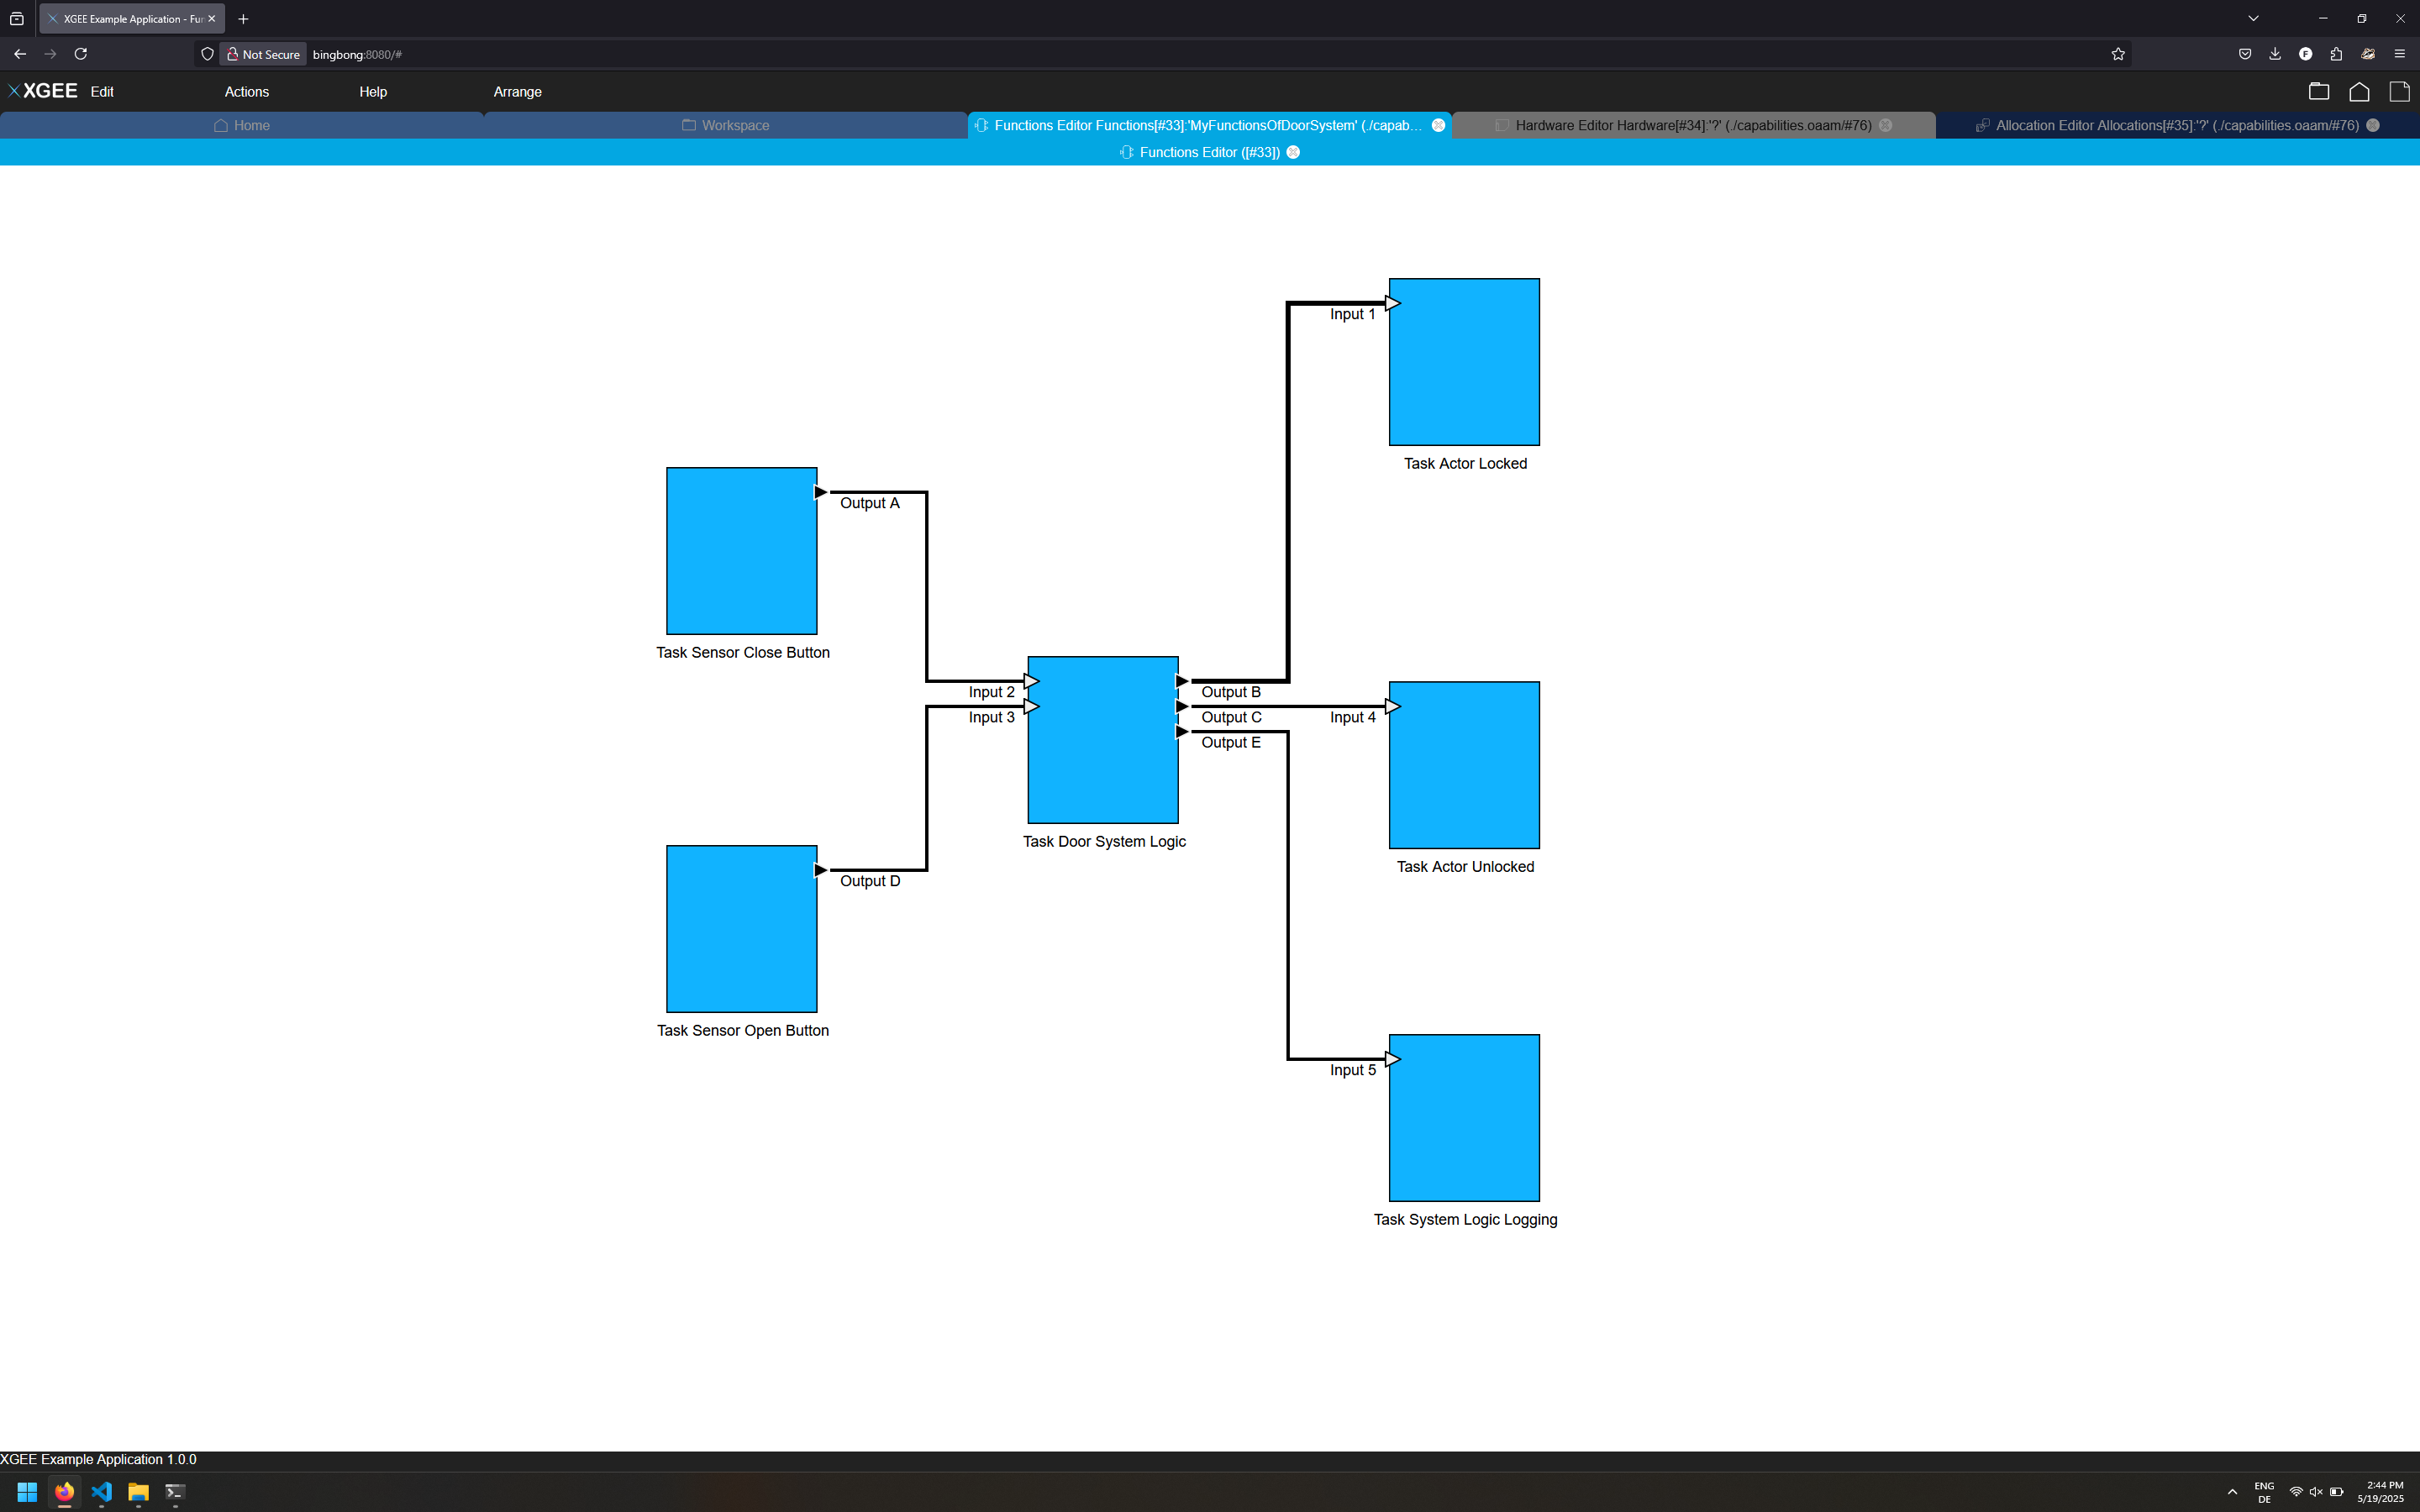
\includegraphics[width=\textwidth]{testcases/edge_2px_too_wide/144434-620311_input_image.png}
        \caption*{\textit{Before}}
    \end{subfigure}
    \newline    
    \begin{subfigure}[t]{0.9\textwidth}
        \centering
        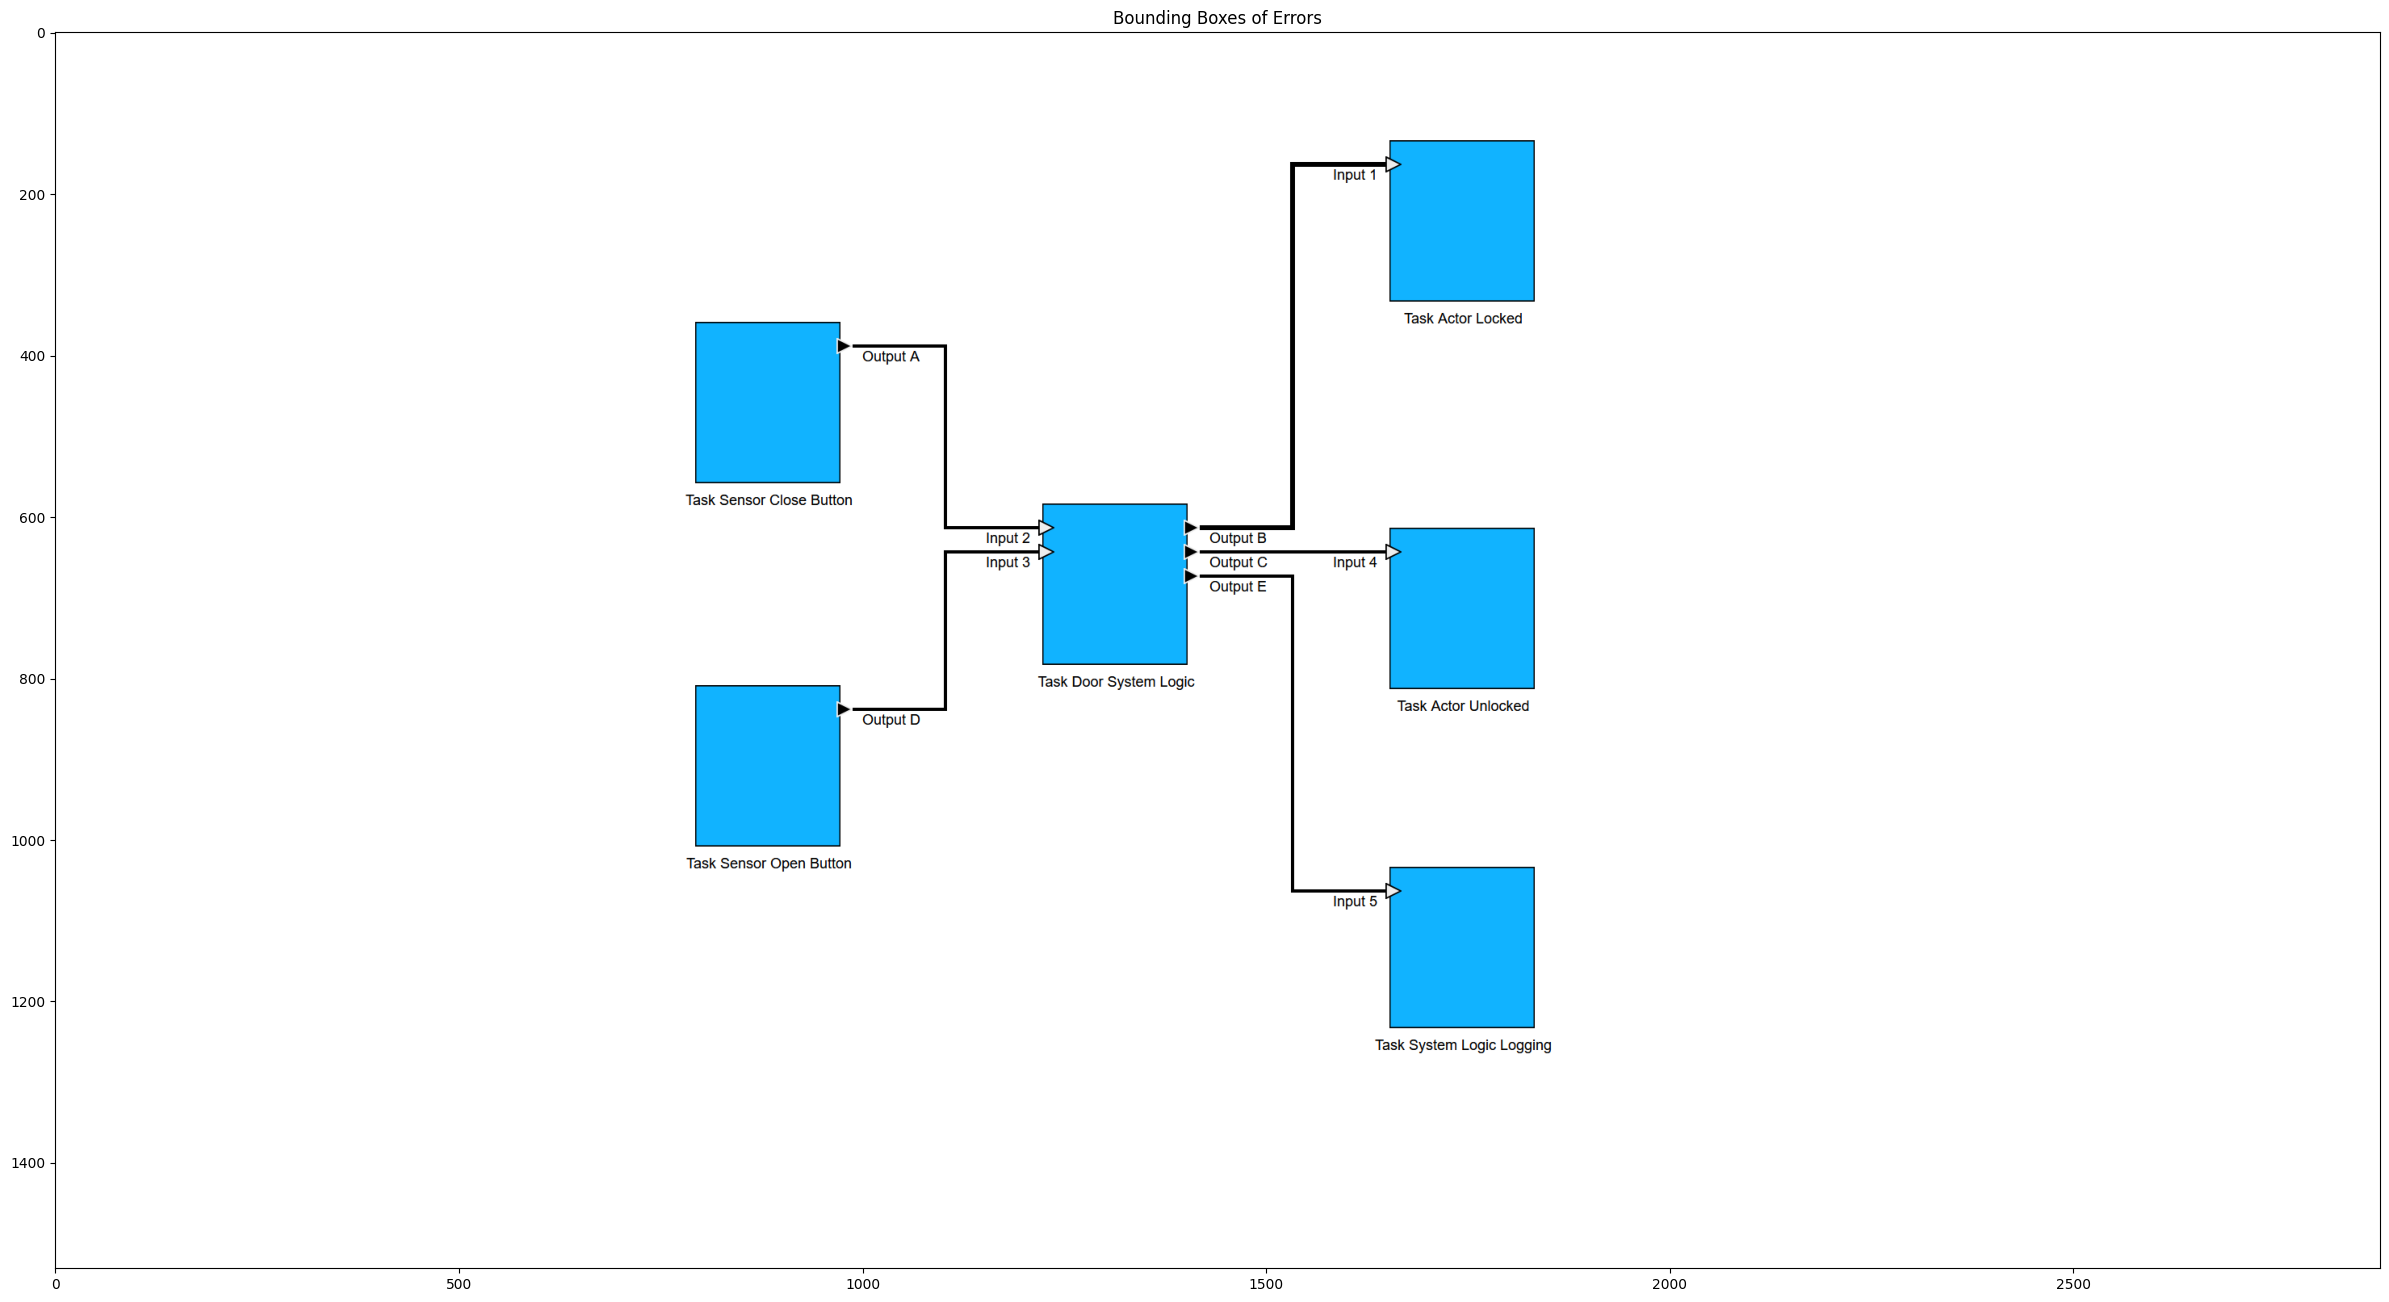
\includegraphics[width=\textwidth]{testcases/edge_2px_too_wide/144456-554148_element_bbox_errors_labeled_colored.png}
        \caption*{\textit{After}}
    \end{subfigure}
    % \caption{Edge too wide}
    \label{fig:edge_too_wide_2}
\end{figure}
\newpage

\section{Edge 3px too wide}
\begin{figure}[H]
    \centering
    \begin{subfigure}[t]{0.9\textwidth}
        \centering
        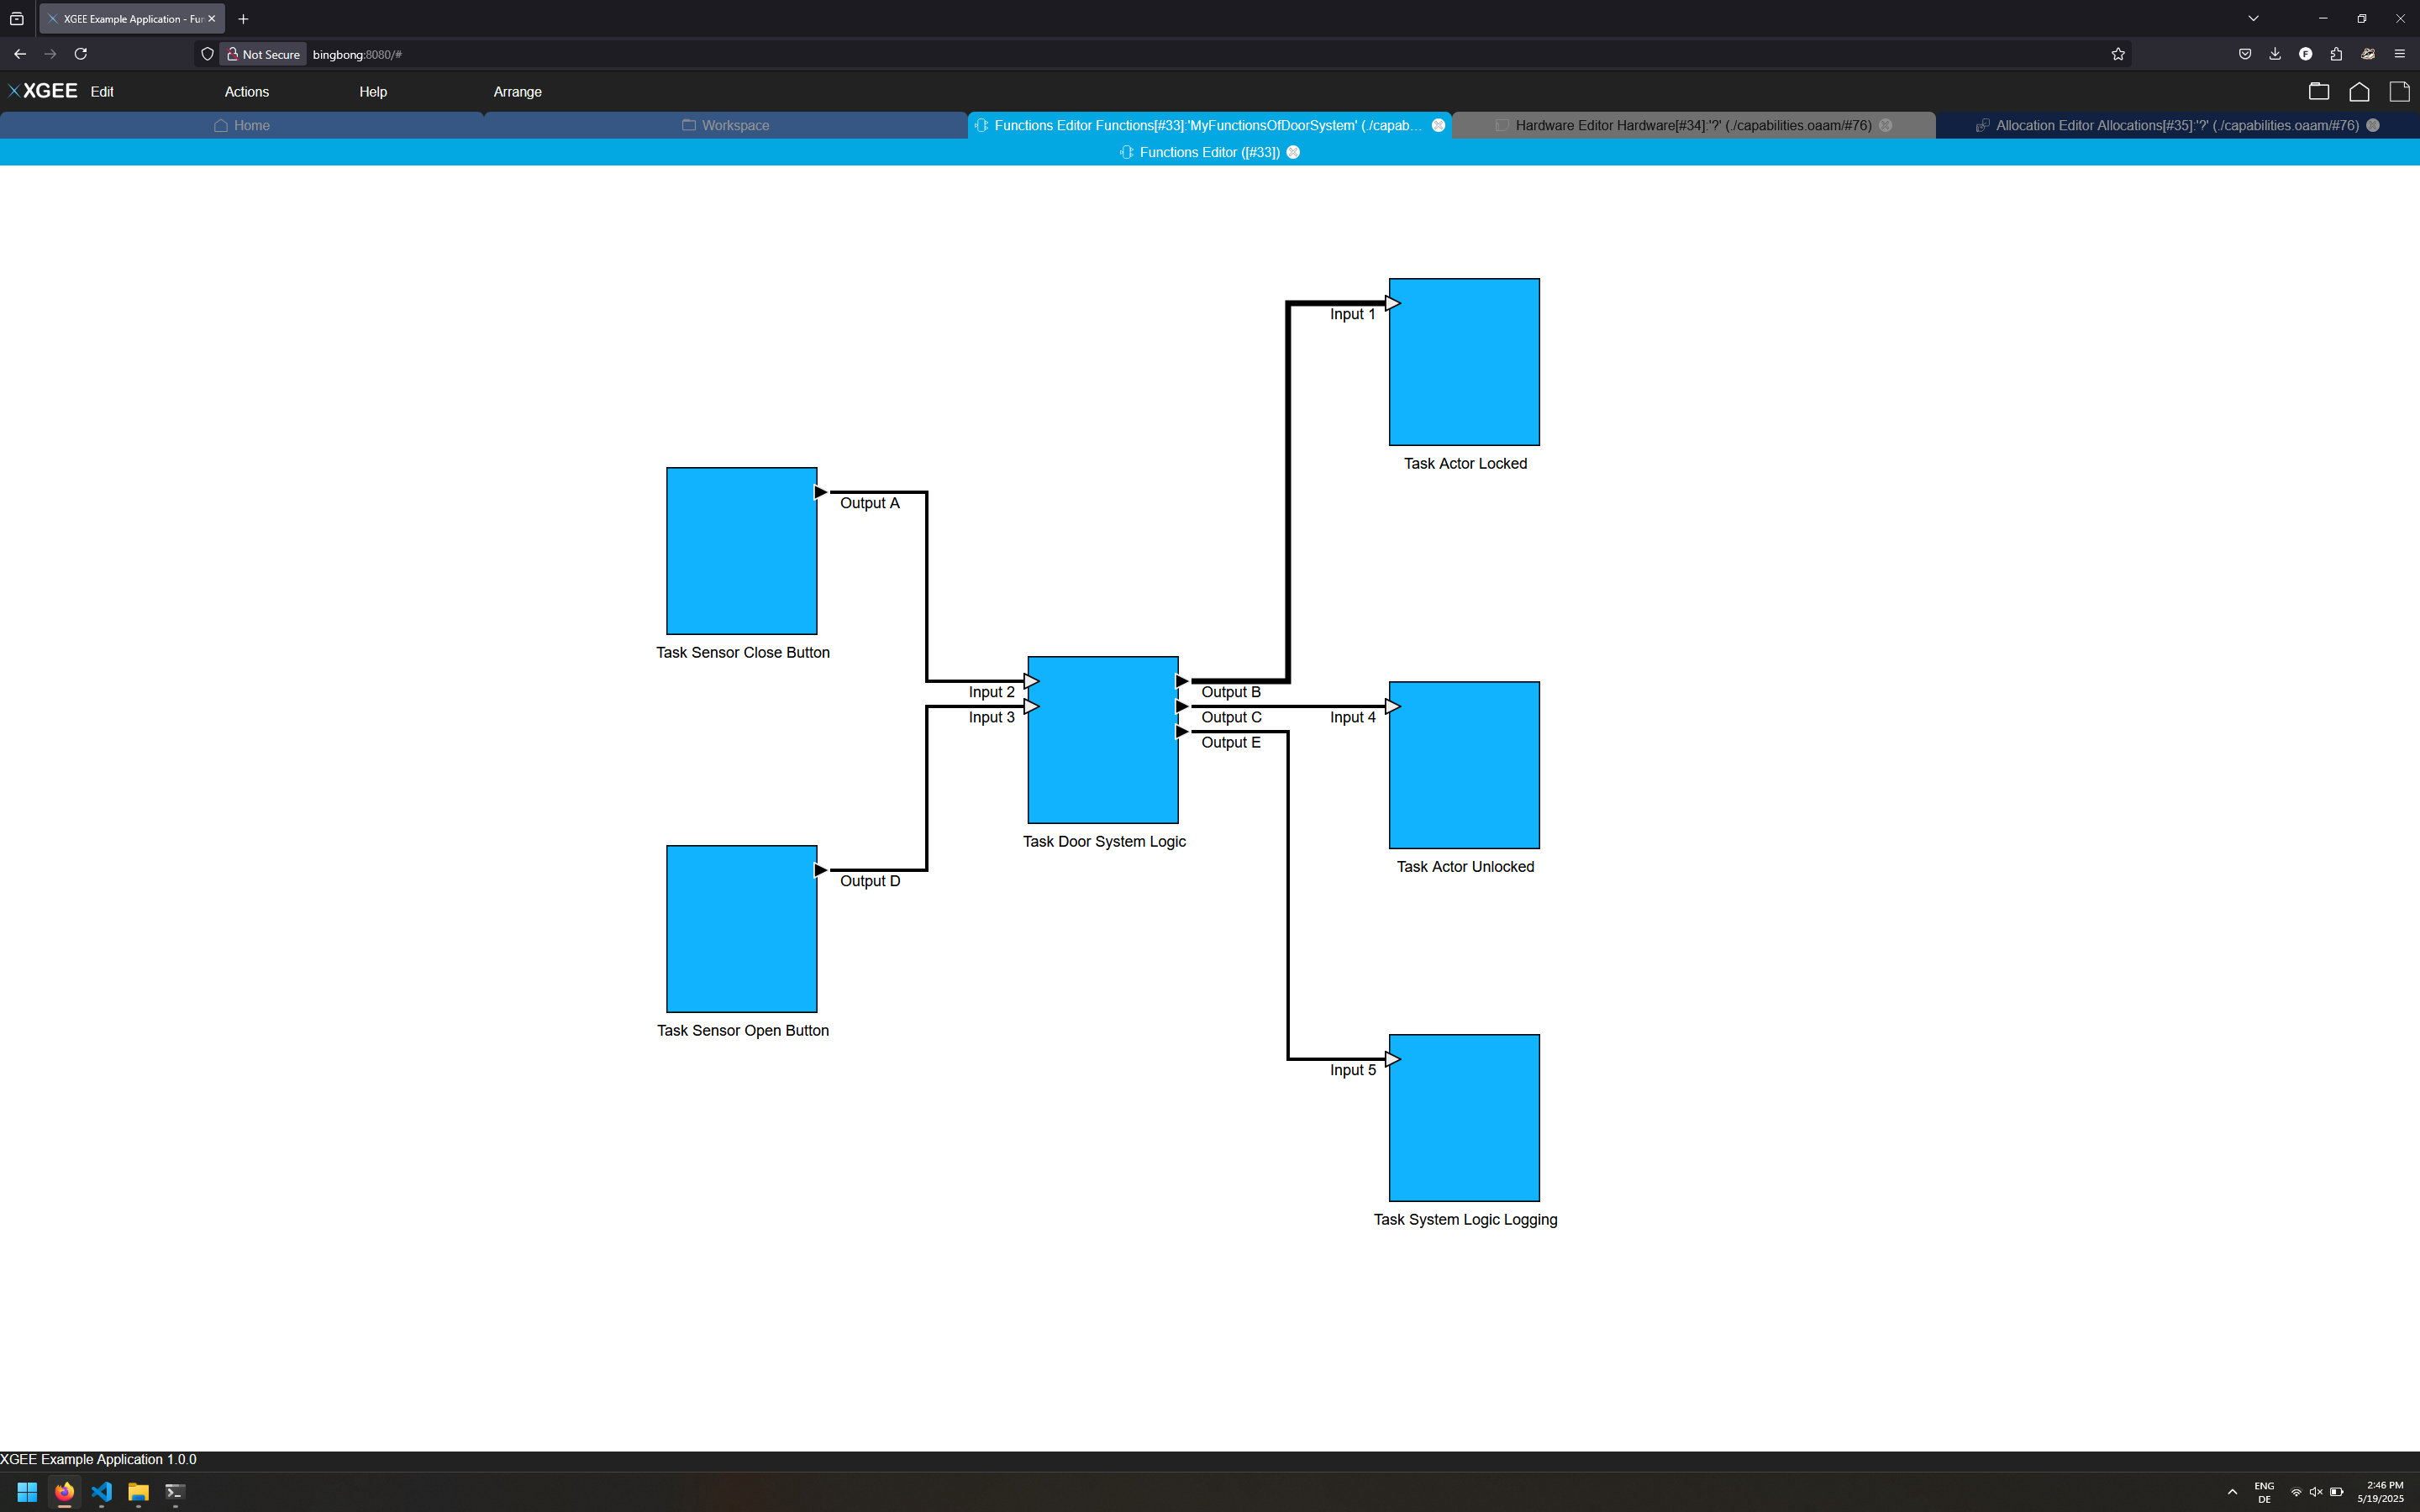
\includegraphics[width=\textwidth]{testcases/edge_3px_too_wide/144613-921105_input_image.png}
        \caption*{\textit{Before}}
    \end{subfigure}
    \newline    
    \begin{subfigure}[t]{0.9\textwidth}
        \centering
        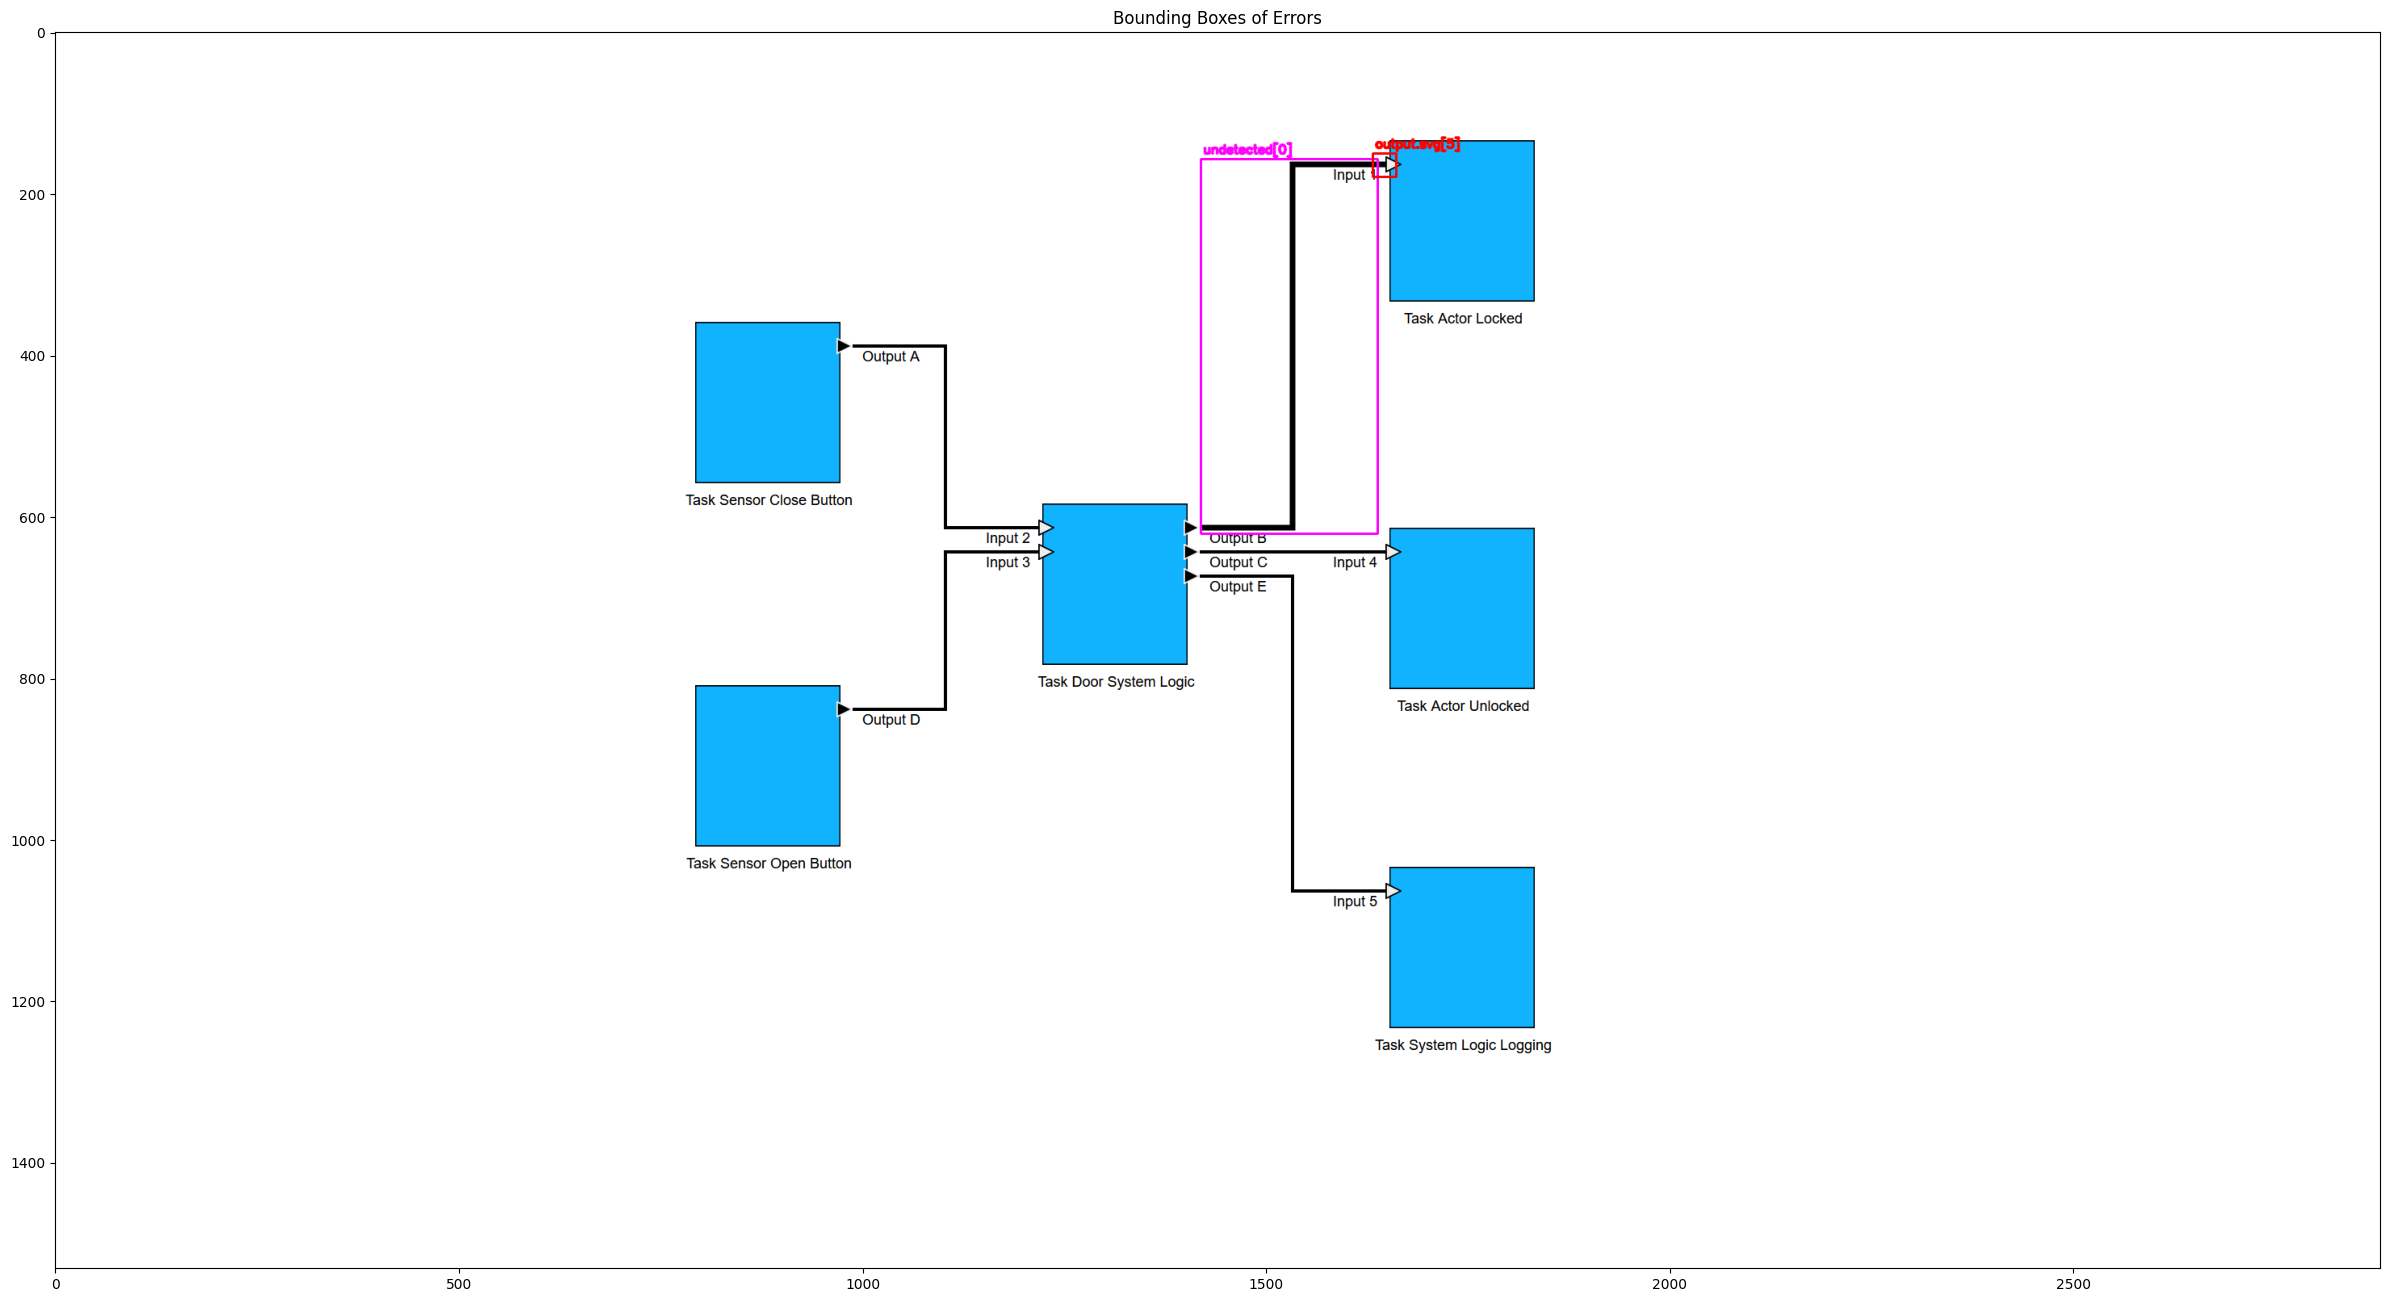
\includegraphics[width=\textwidth]{testcases/edge_3px_too_wide/144634-044834_element_bbox_errors_labeled_colored.png}
        \caption*{\textit{After}}
    \end{subfigure}
    % \caption{Edge too wide}
    \label{fig:edge_too_wide_3}
\end{figure}
\newpage

\section{Edge wrong color}
\begin{figure}[H]
    \centering
    \begin{subfigure}[t]{0.9\textwidth}
        \centering
        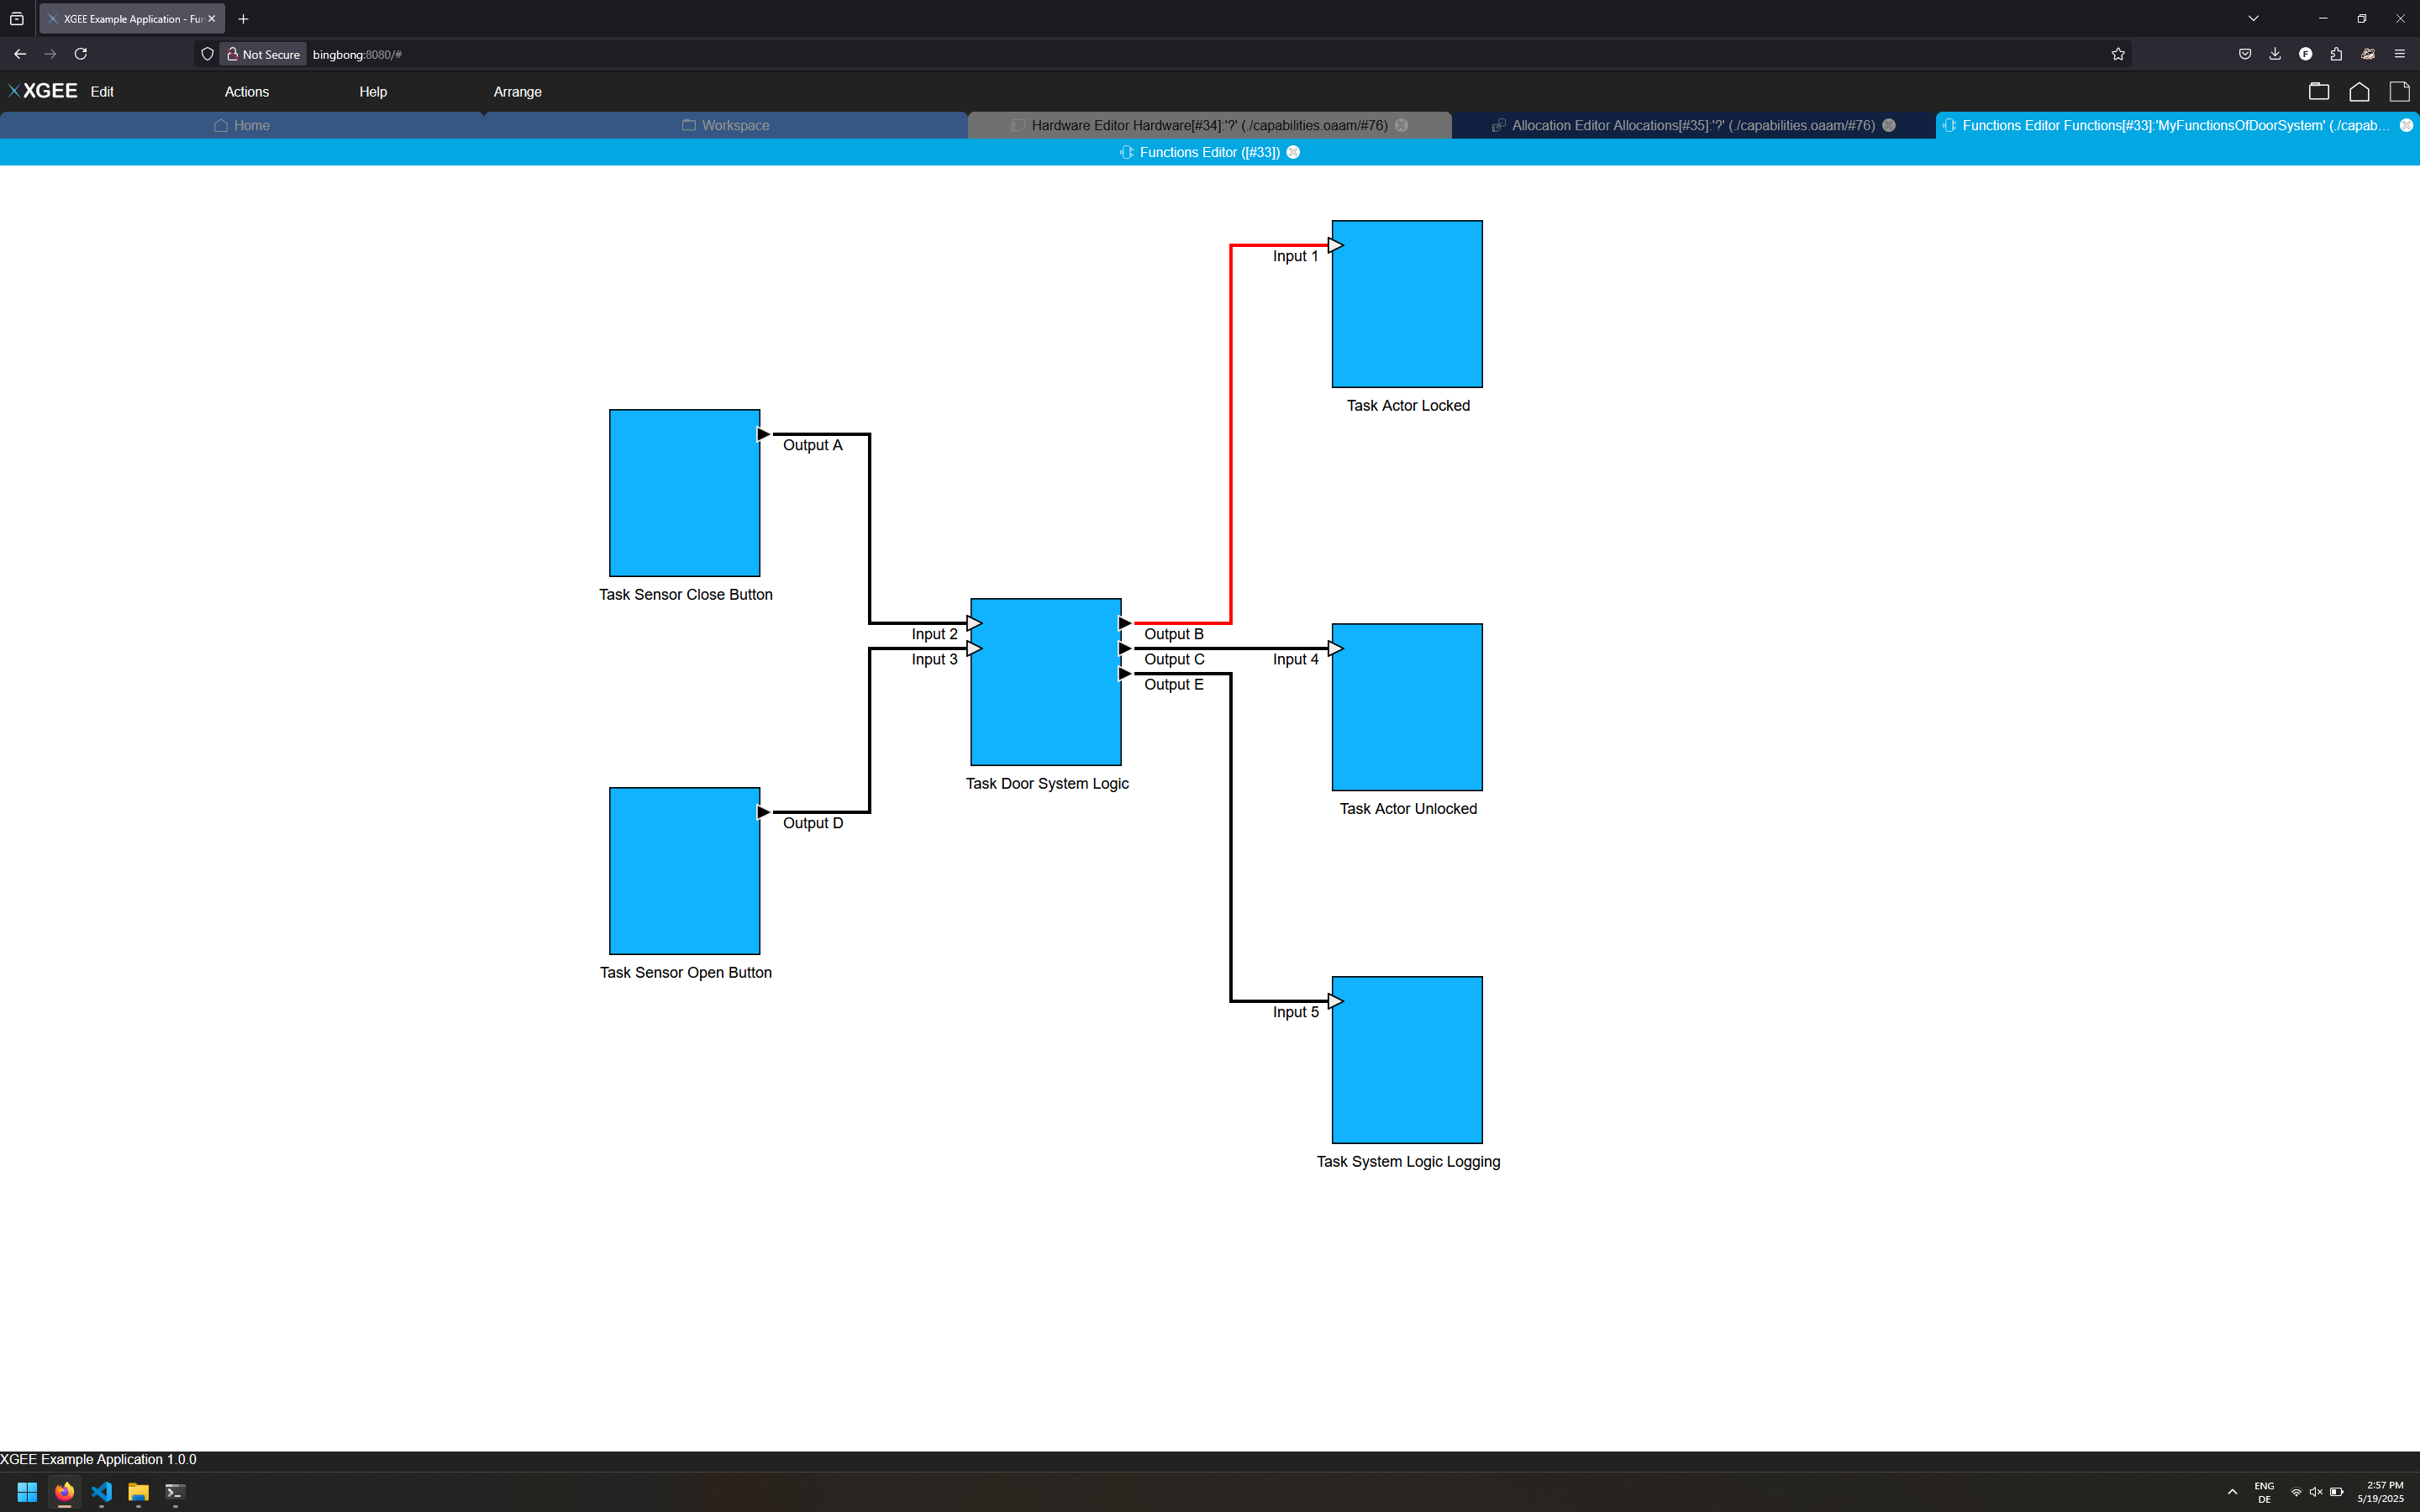
\includegraphics[width=\textwidth]{testcases/edge_wrong_color/145759-936864_input_image.png}
        \caption*{\textit{Before}}
    \end{subfigure}
    \newline    
    \begin{subfigure}[t]{0.9\textwidth}
        \centering
        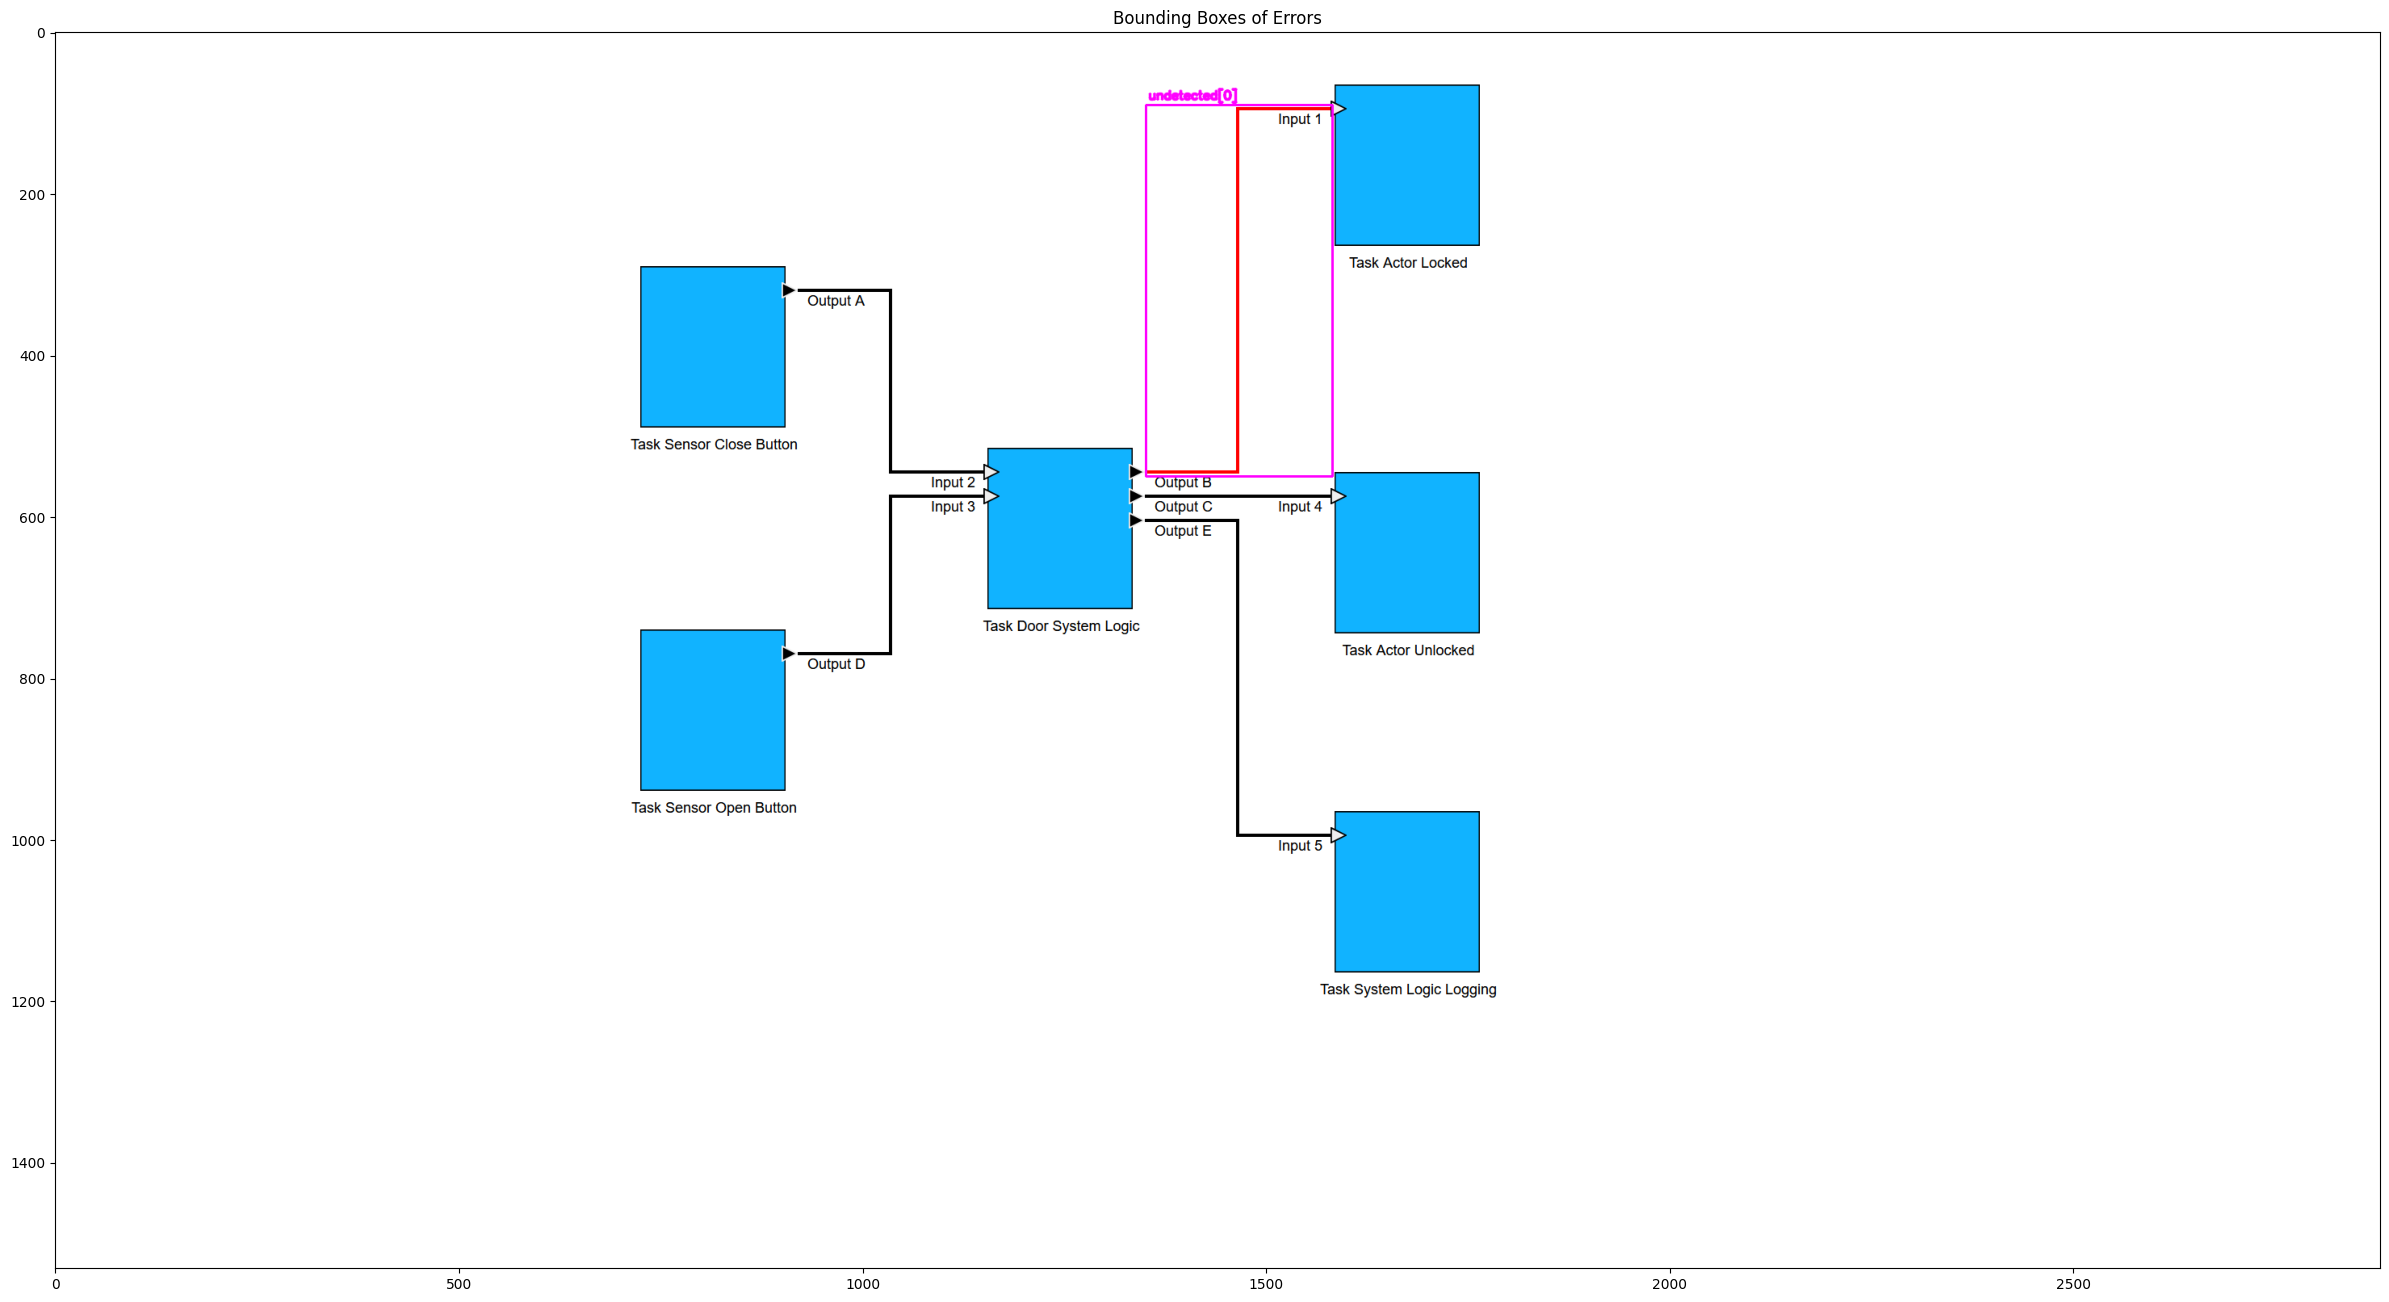
\includegraphics[width=\textwidth]{testcases/edge_wrong_color/145820-255866_element_bbox_errors_labeled_colored.png}
        \caption*{\textit{After}}
    \end{subfigure}
    % \caption{Edge wrong color}
    \label{fig:edge_wrong_color}
\end{figure}
\newpage

\section{Edge 10px too high}
\begin{figure}[H]
    \centering
    \begin{subfigure}[t]{0.9\textwidth}
        \centering
        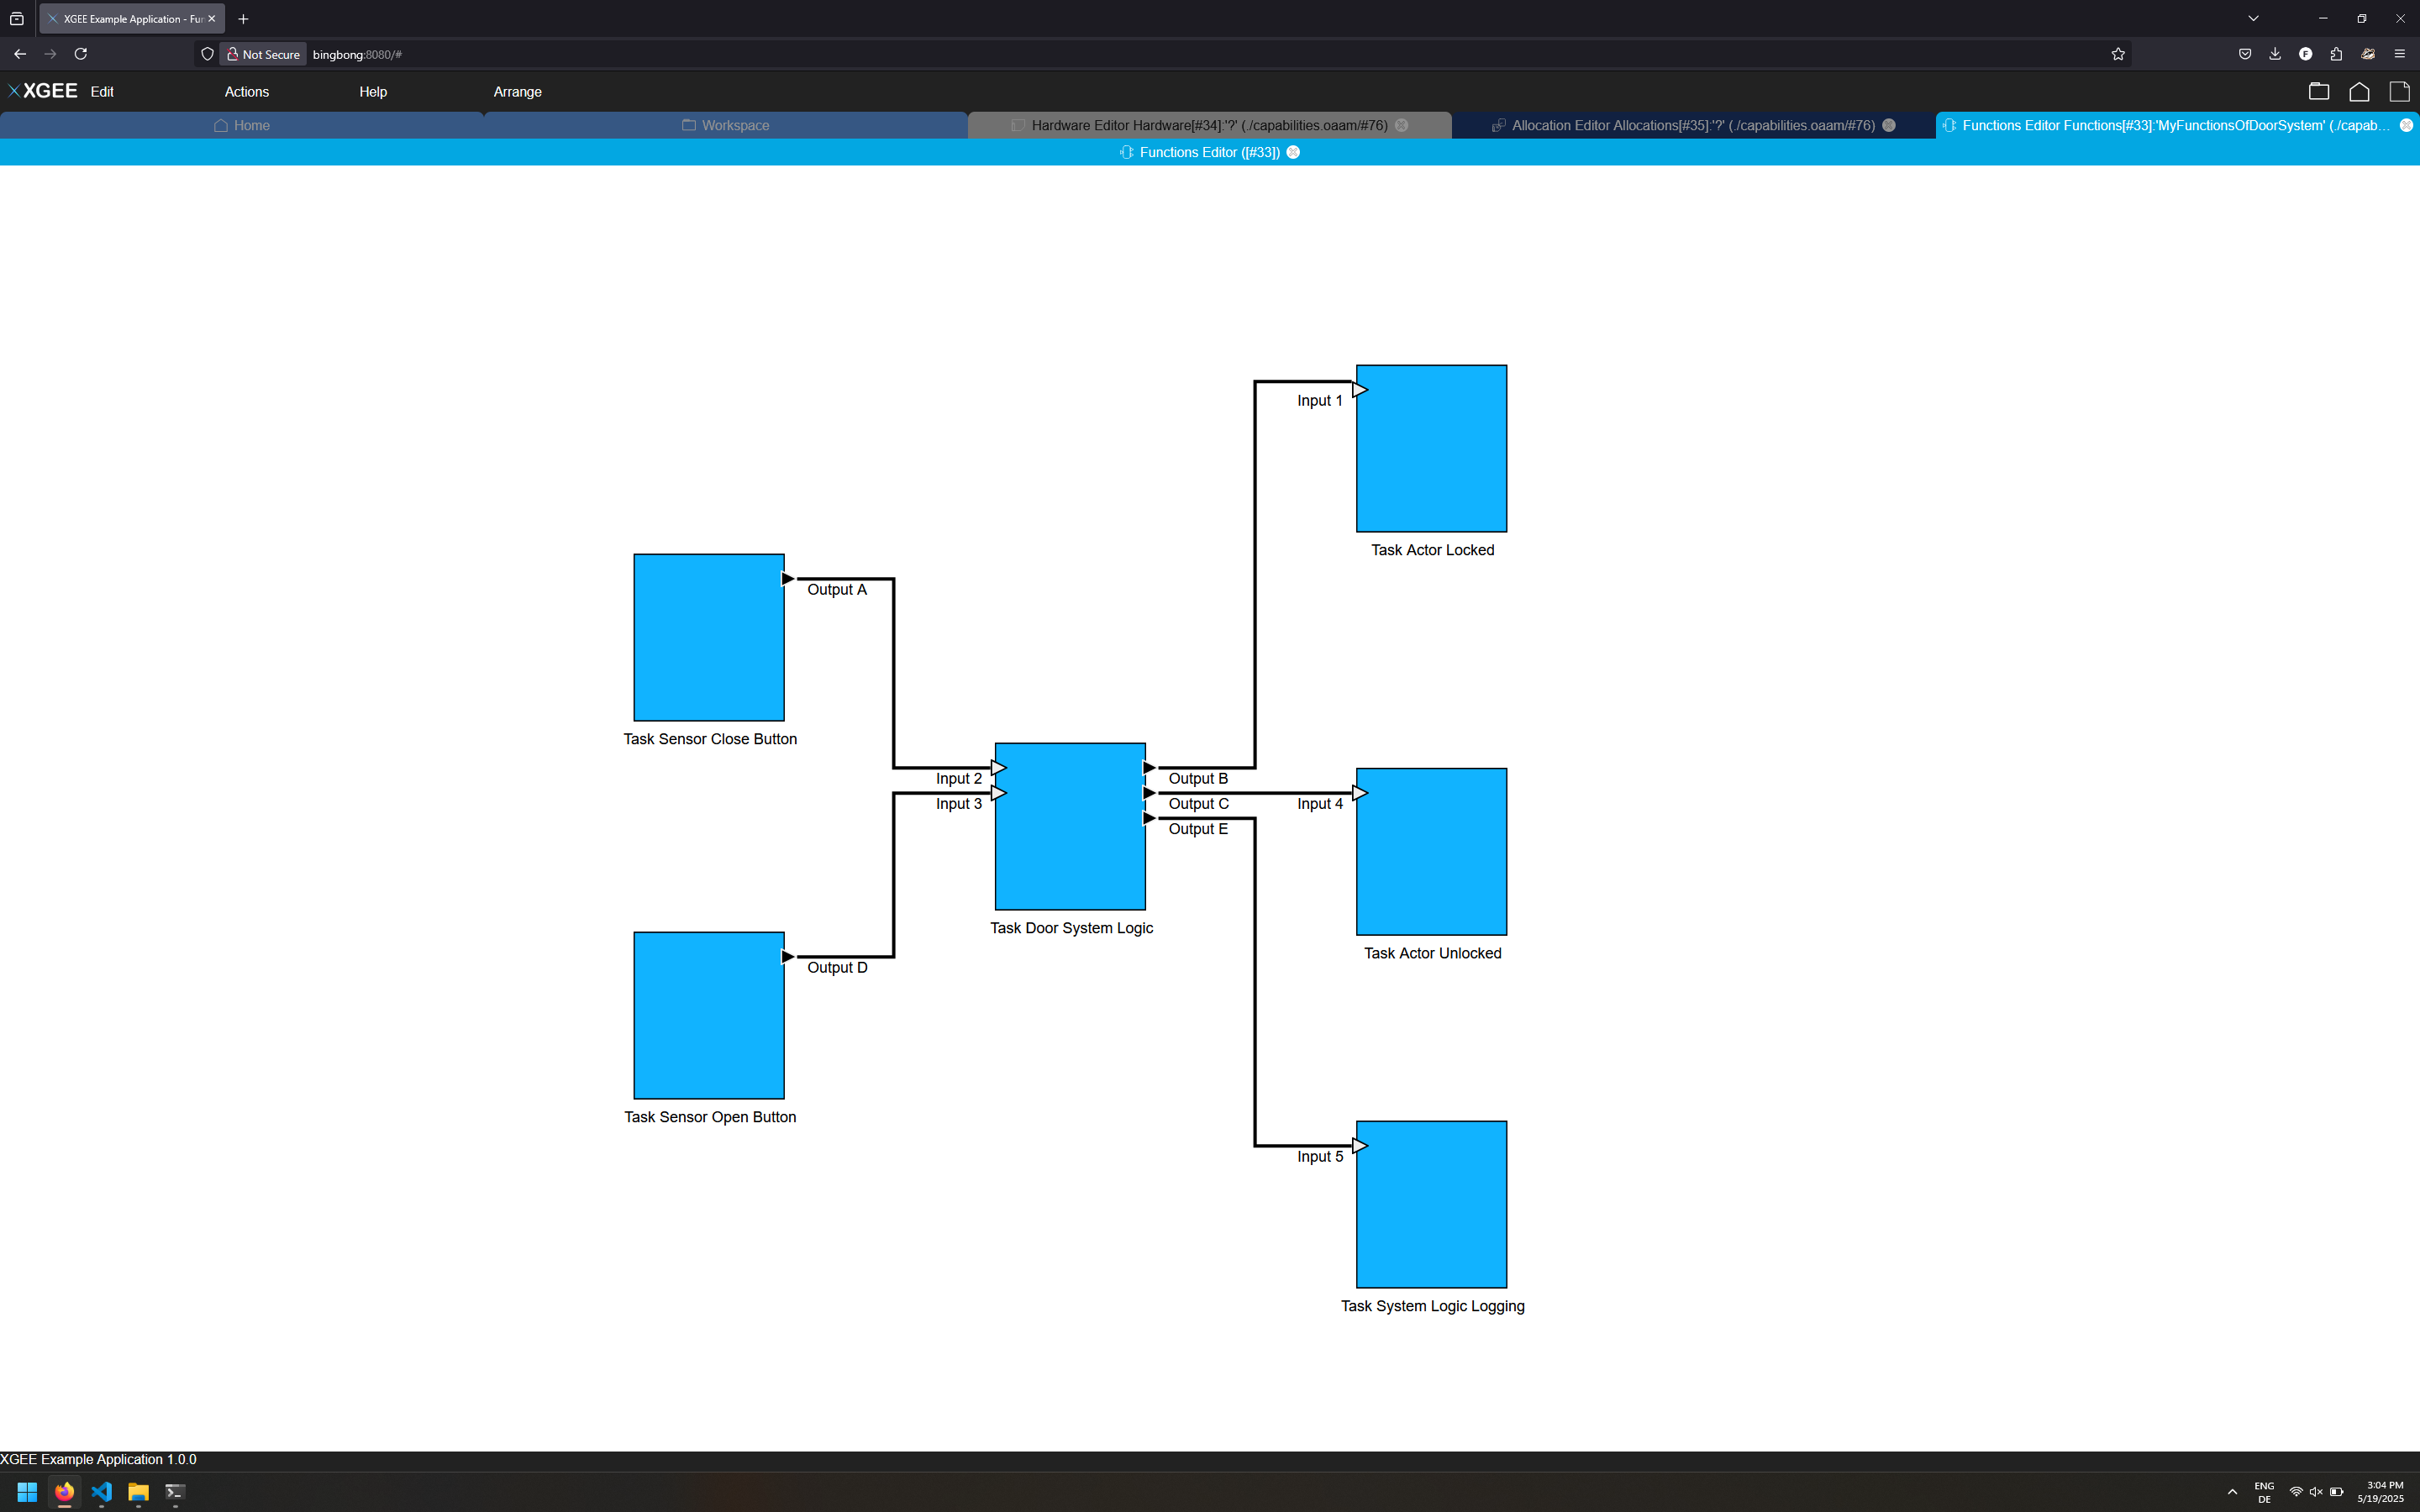
\includegraphics[width=\textwidth]{testcases/edge_10px_too_high/150452-500412_input_image.png}
        \caption*{\textit{Before}}
    \end{subfigure}
    \newline    
    \begin{subfigure}[t]{0.9\textwidth}
        \centering
        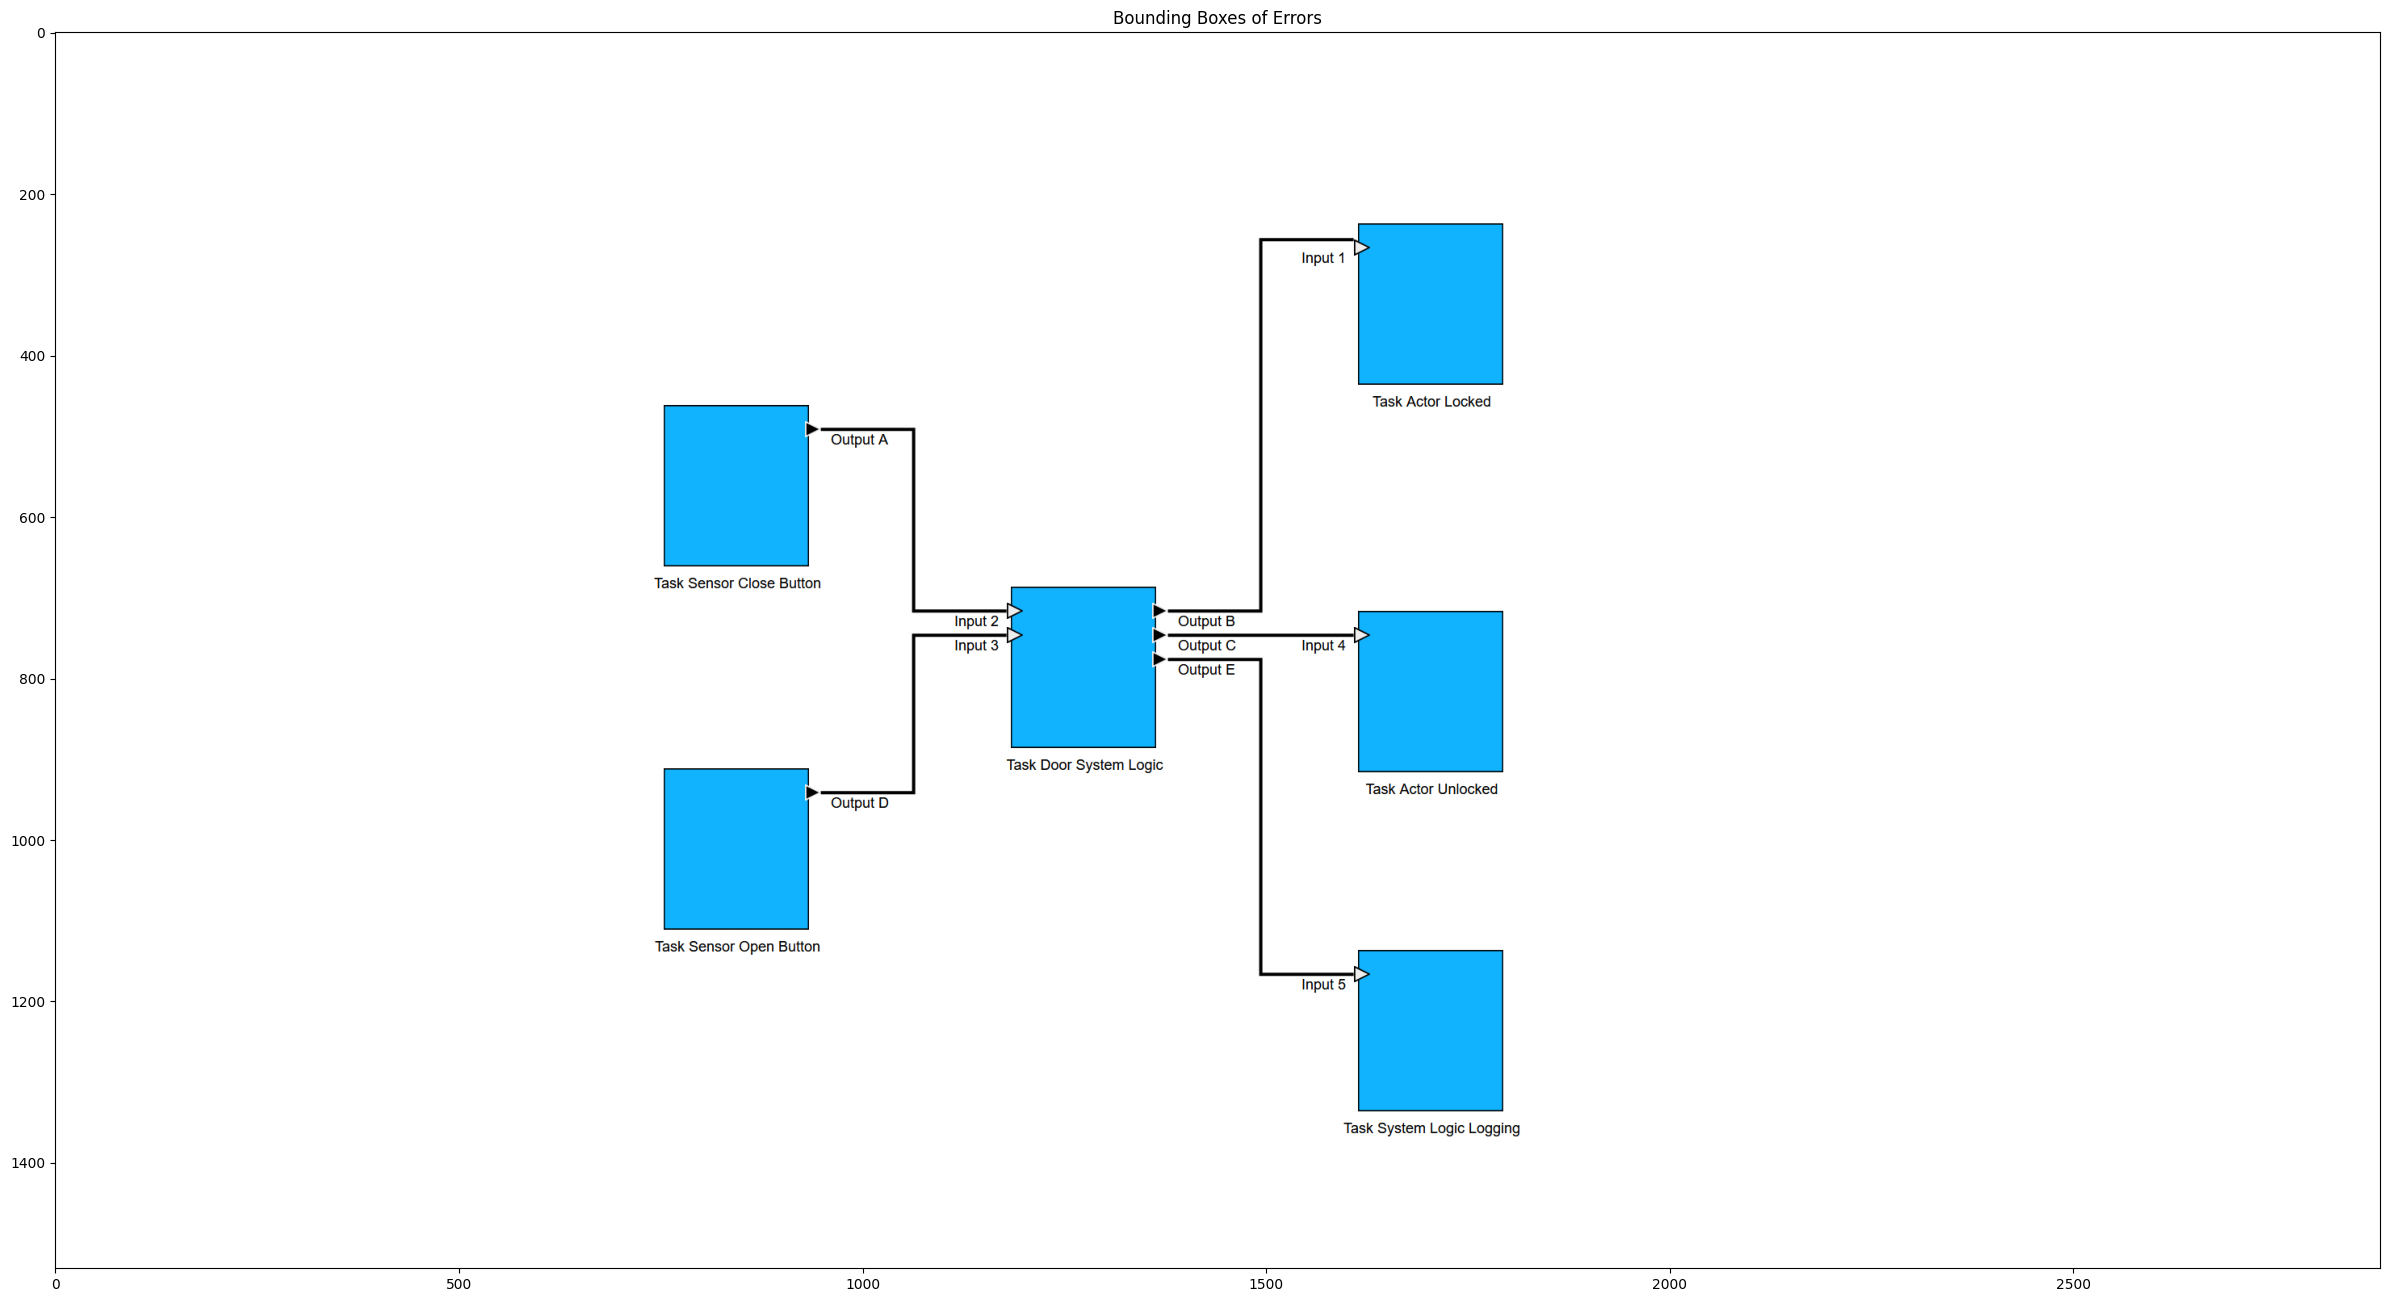
\includegraphics[width=\textwidth]{testcases/edge_10px_too_high/150513-636204_element_bbox_errors_labeled_colored.png}
        \caption*{\textit{After}}
    \end{subfigure}
    % \caption{Edge}
    \label{fig:edge_too_high_10}
\end{figure}
\newpage

\section{Edge 20px too high}
\begin{figure}[H]
    \centering
    \begin{subfigure}[t]{0.9\textwidth}
        \centering
        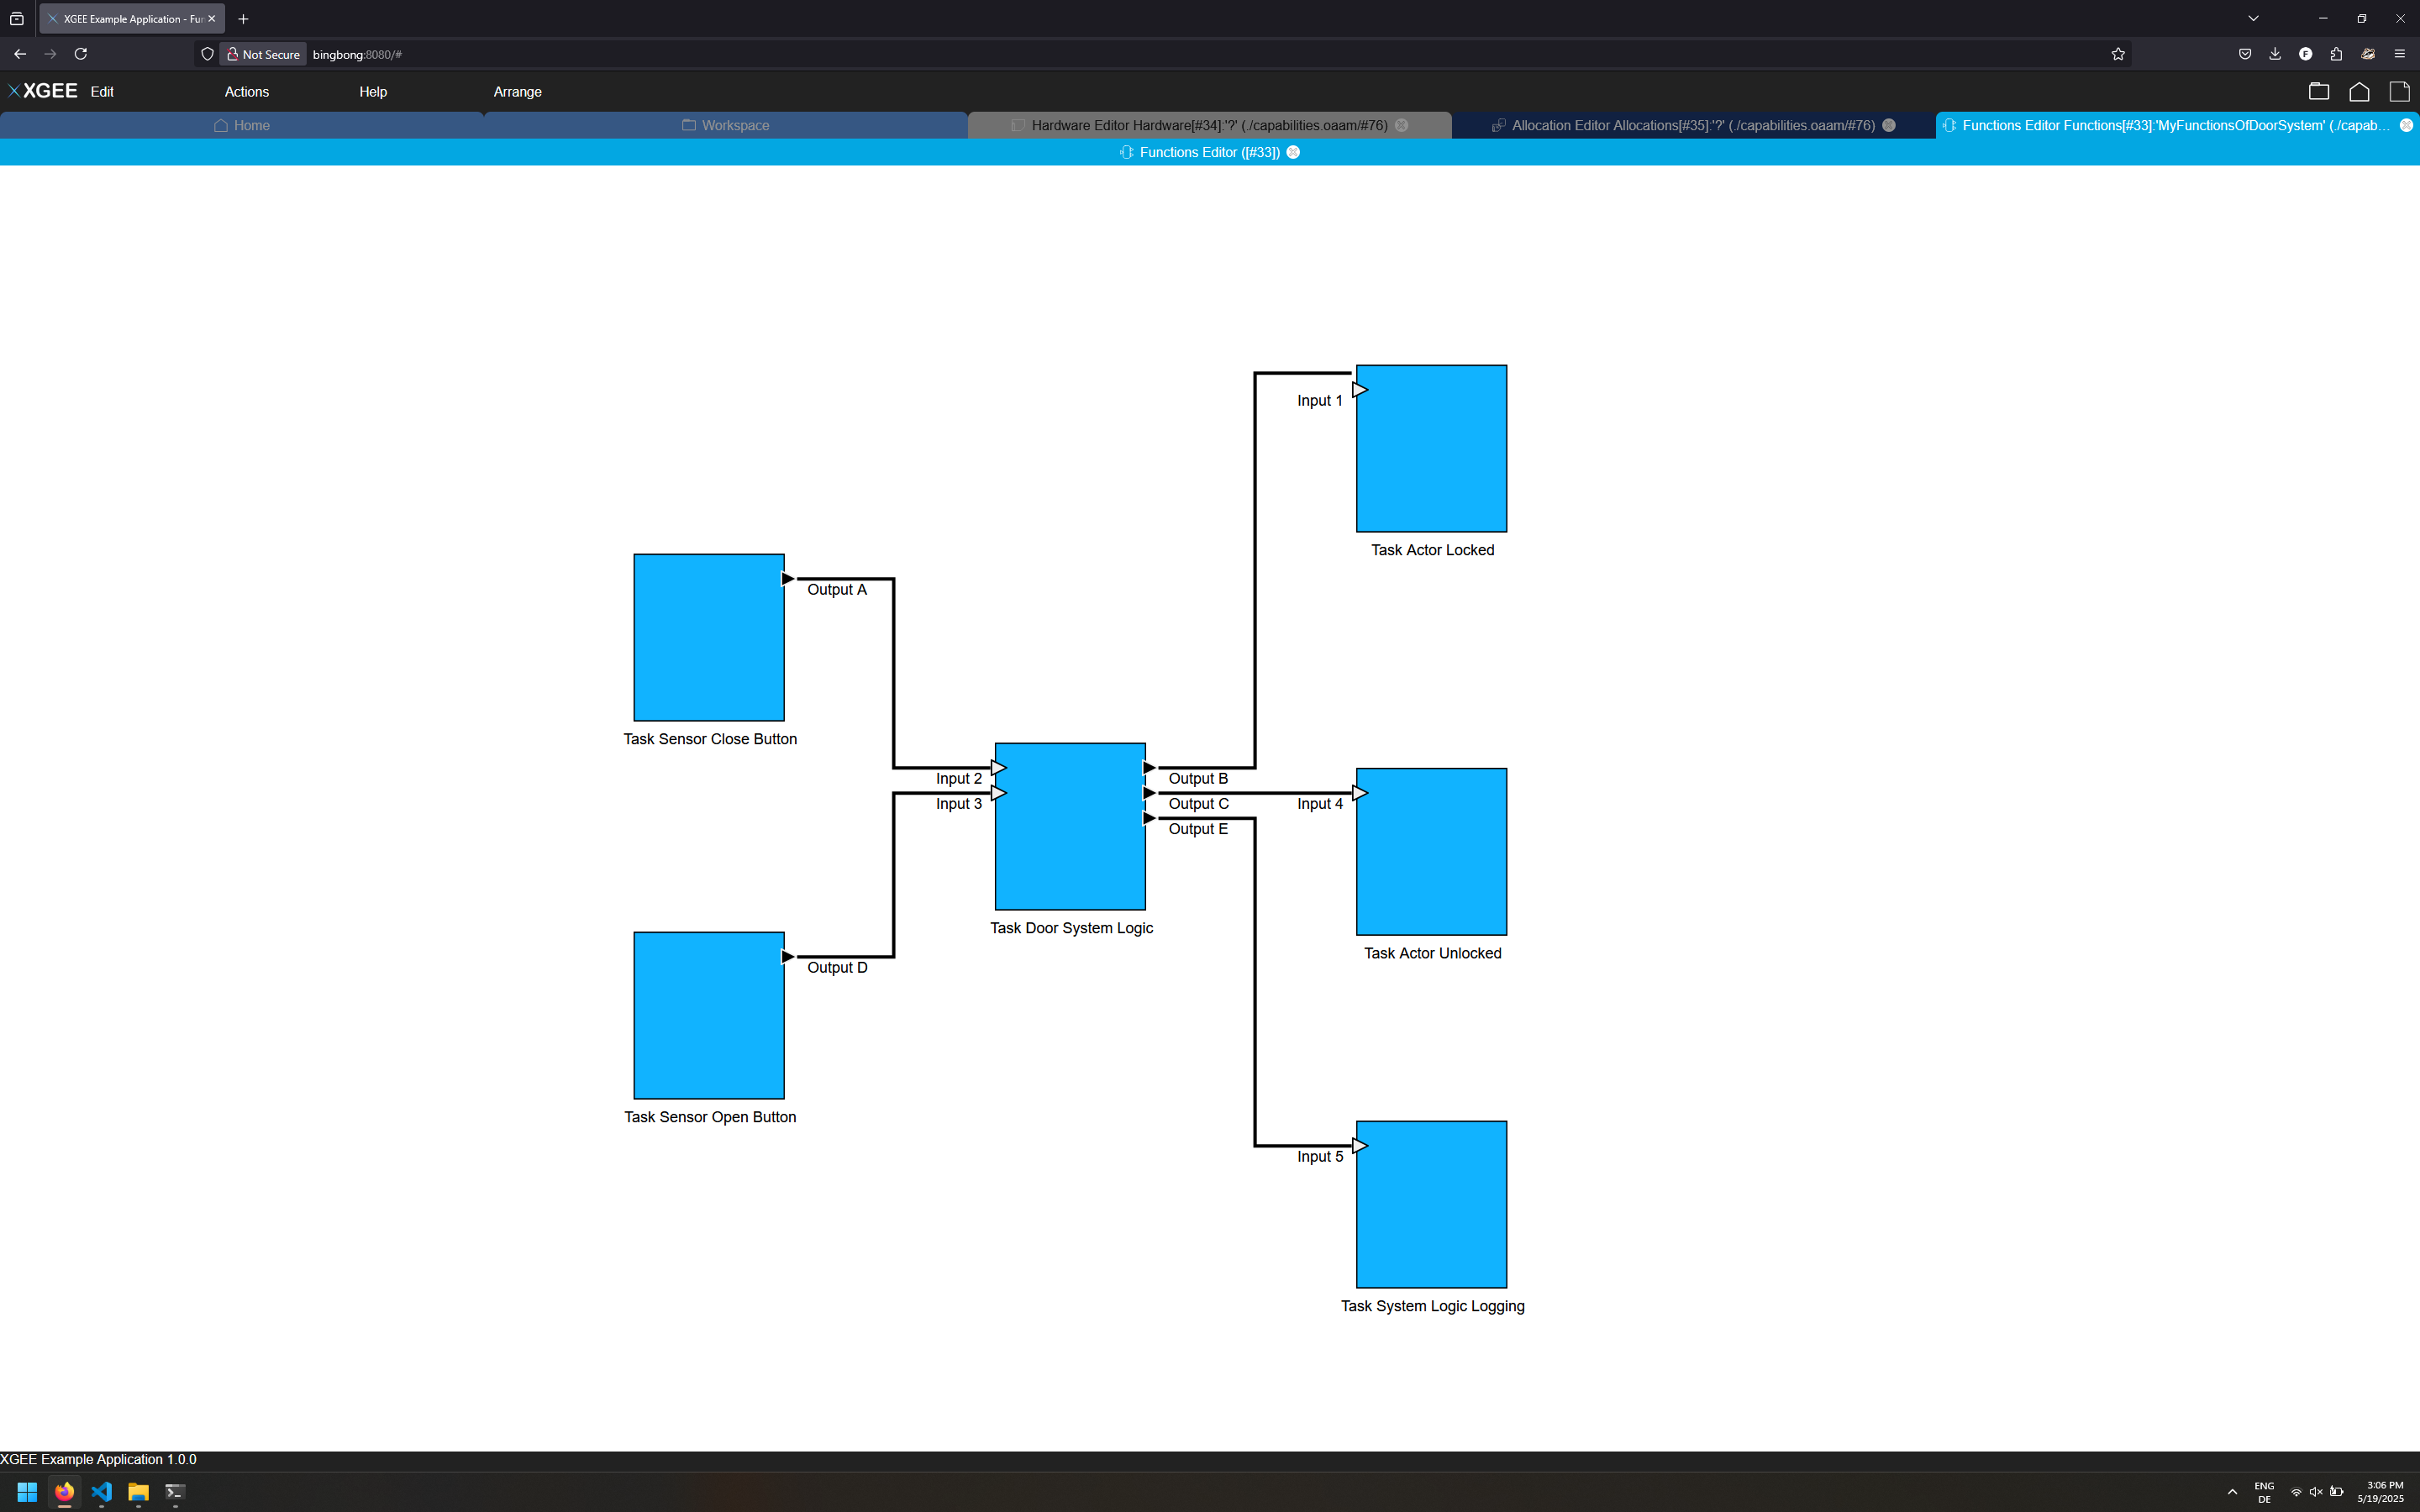
\includegraphics[width=\textwidth]{testcases/edge_20px_too_high/150645-838295_input_image.png}
        \caption*{\textit{Before}}
    \end{subfigure}
    \newline    
    \begin{subfigure}[t]{0.9\textwidth}
        \centering
        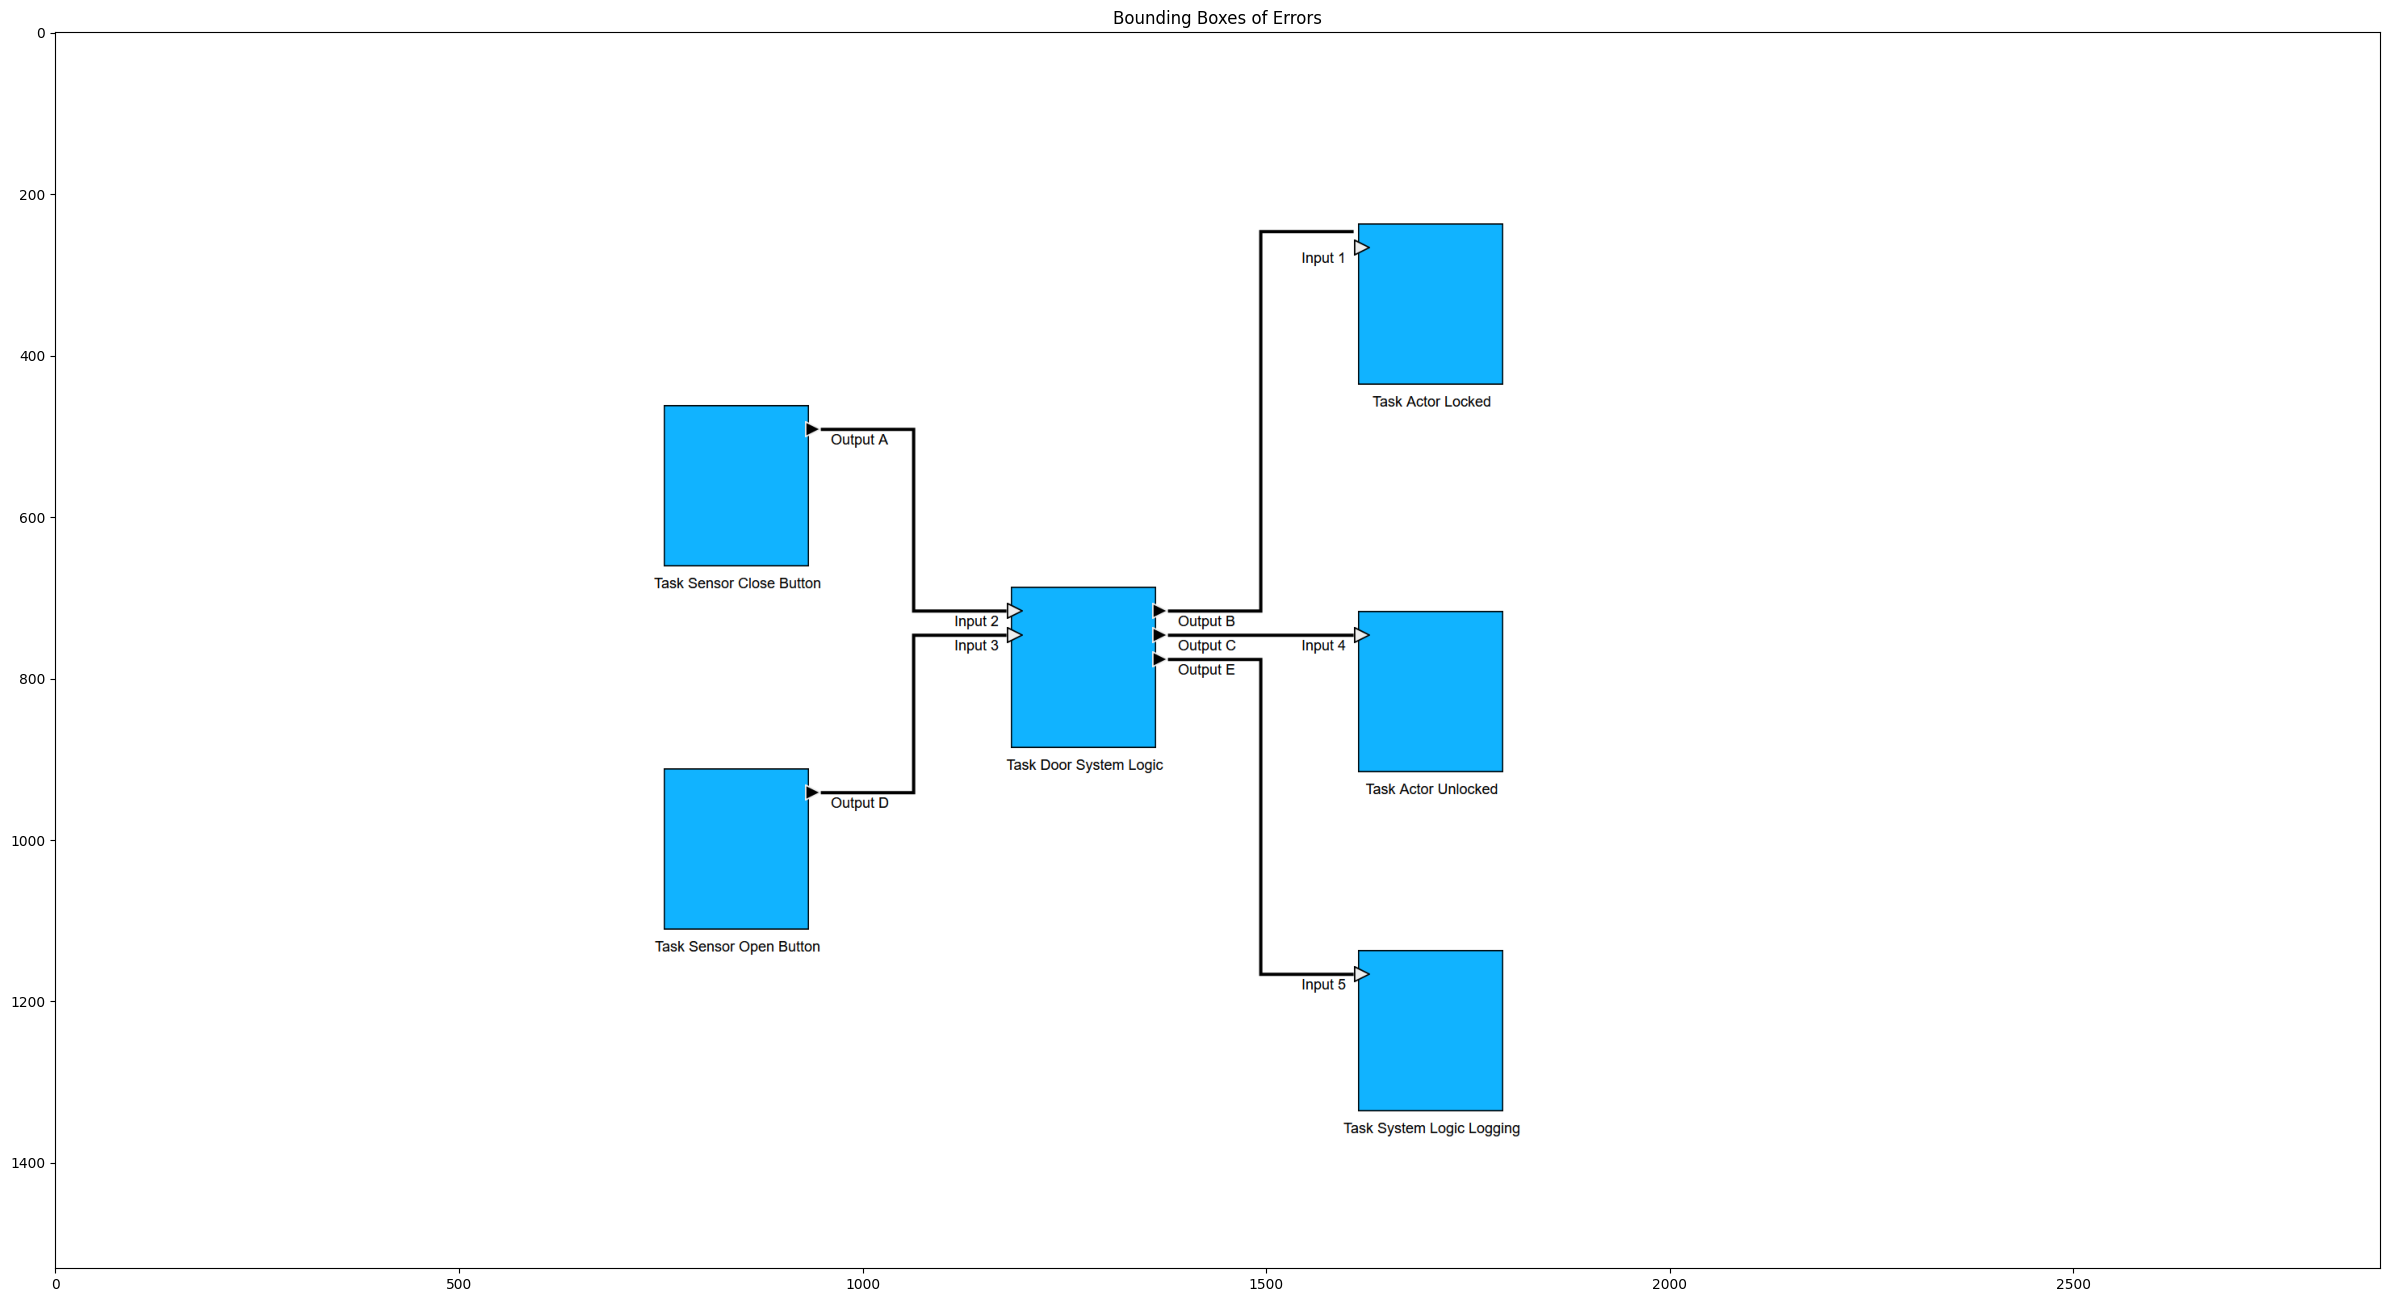
\includegraphics[width=\textwidth]{testcases/edge_20px_too_high/150658-463094_element_bbox_errors_labeled_colored.png}
        \caption*{\textit{After}}
    \end{subfigure}
    % \caption{Edge}
    \label{fig:edge_too_high_20}
\end{figure}
\newpage

\section{Edge 30px too high}
\begin{figure}[H]
    \centering
    \begin{subfigure}[t]{0.9\textwidth}
        \centering
        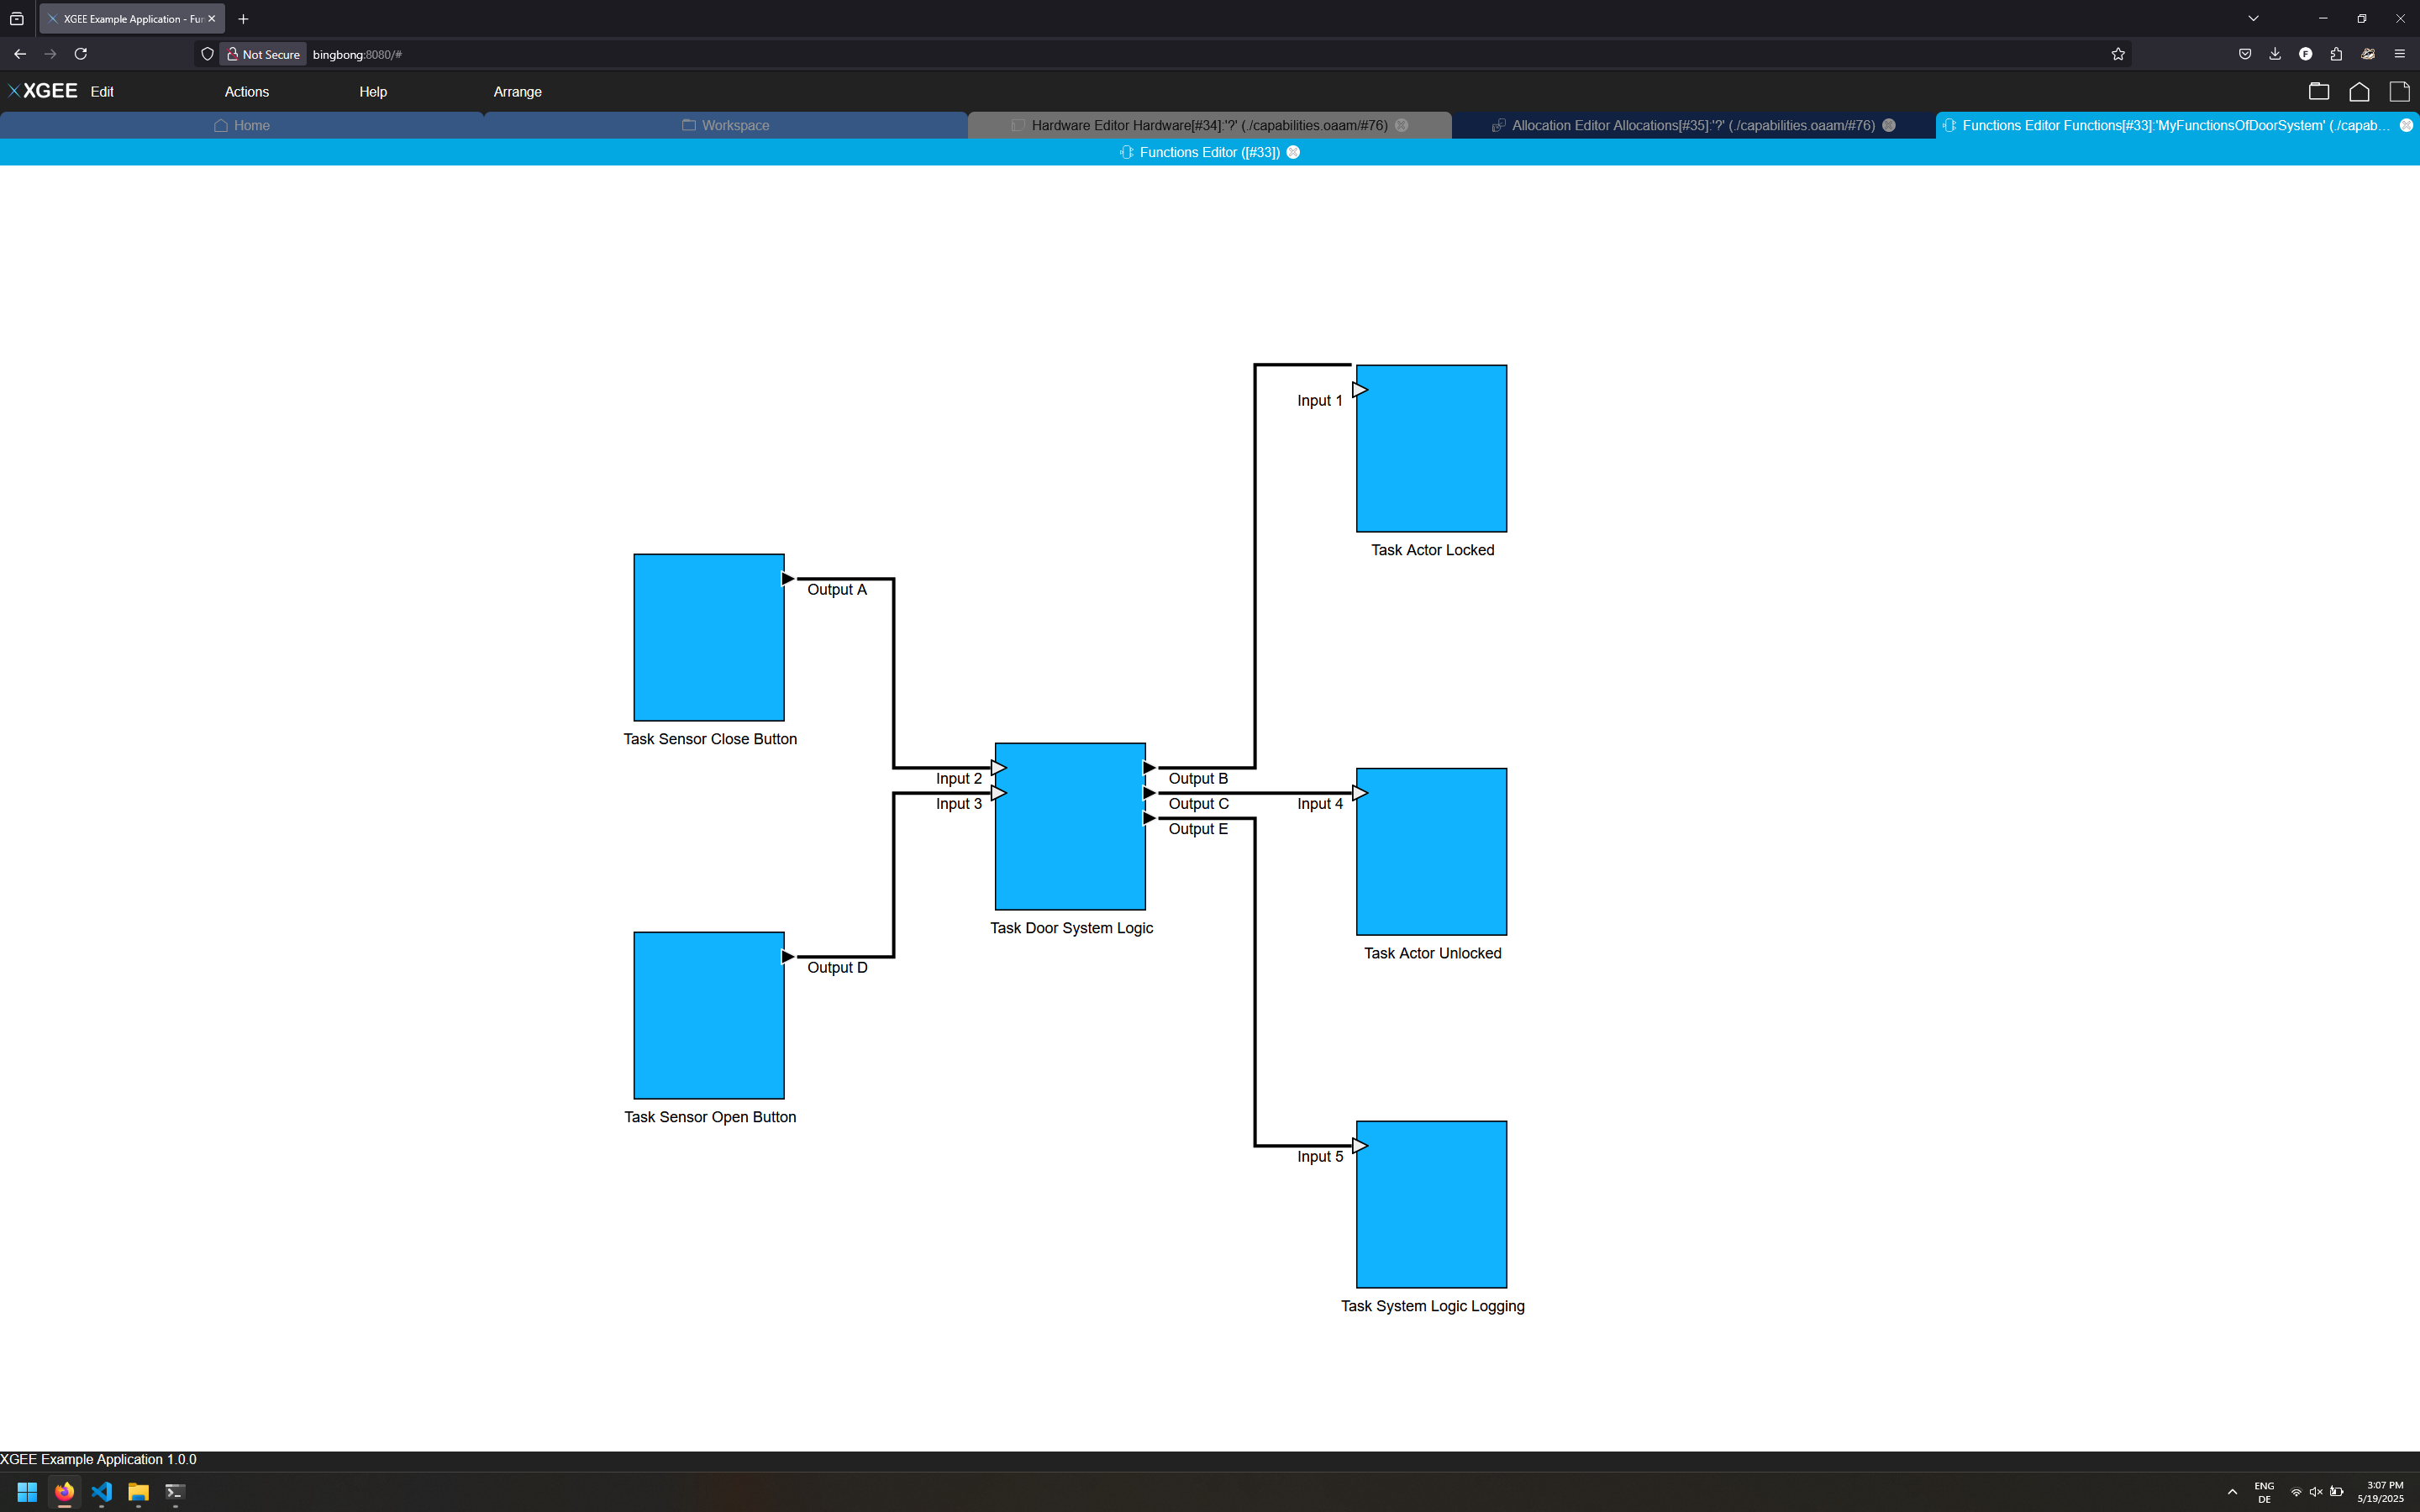
\includegraphics[width=\textwidth]{testcases/edge_30px_too_high/150756-999875_input_image.png}
        \caption*{\textit{Before}}
    \end{subfigure}
    \newline    
    \begin{subfigure}[t]{0.9\textwidth}
        \centering
        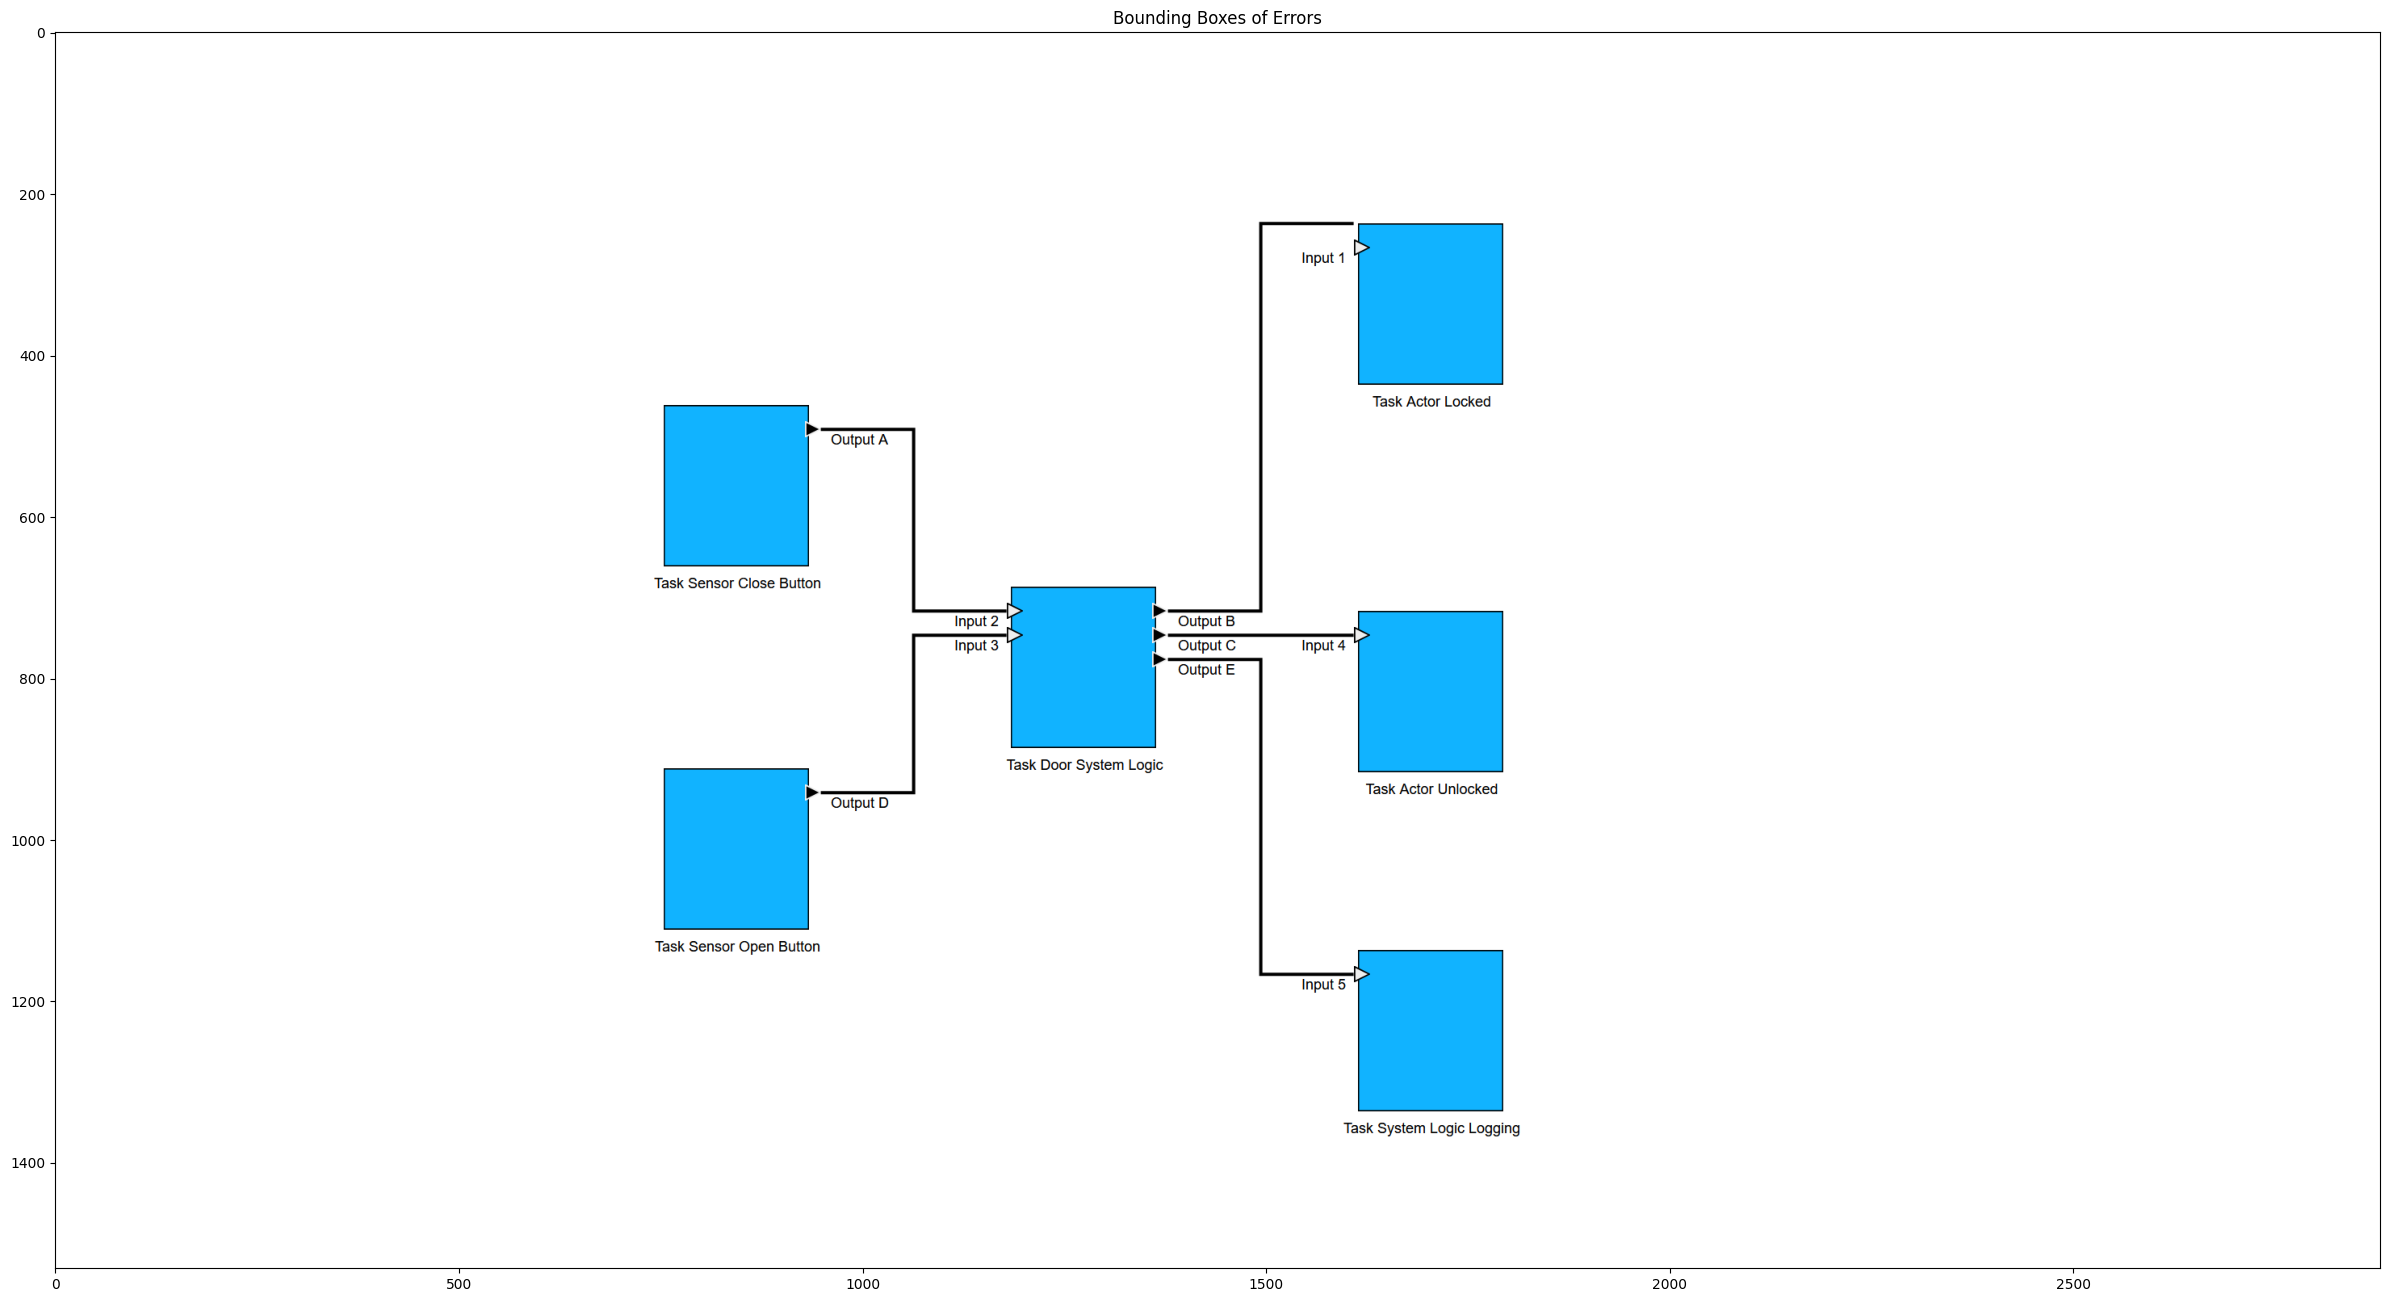
\includegraphics[width=\textwidth]{testcases/edge_30px_too_high/150809-647163_element_bbox_errors_labeled_colored.png}
        \caption*{\textit{After}}
    \end{subfigure}
    % \caption{Edge}
    \label{fig:edge_too_high_30}
\end{figure}
\newpage

\section{Edge 10px too long}
\begin{figure}[H]
    \centering
    \begin{subfigure}[t]{0.9\textwidth}
        \centering
        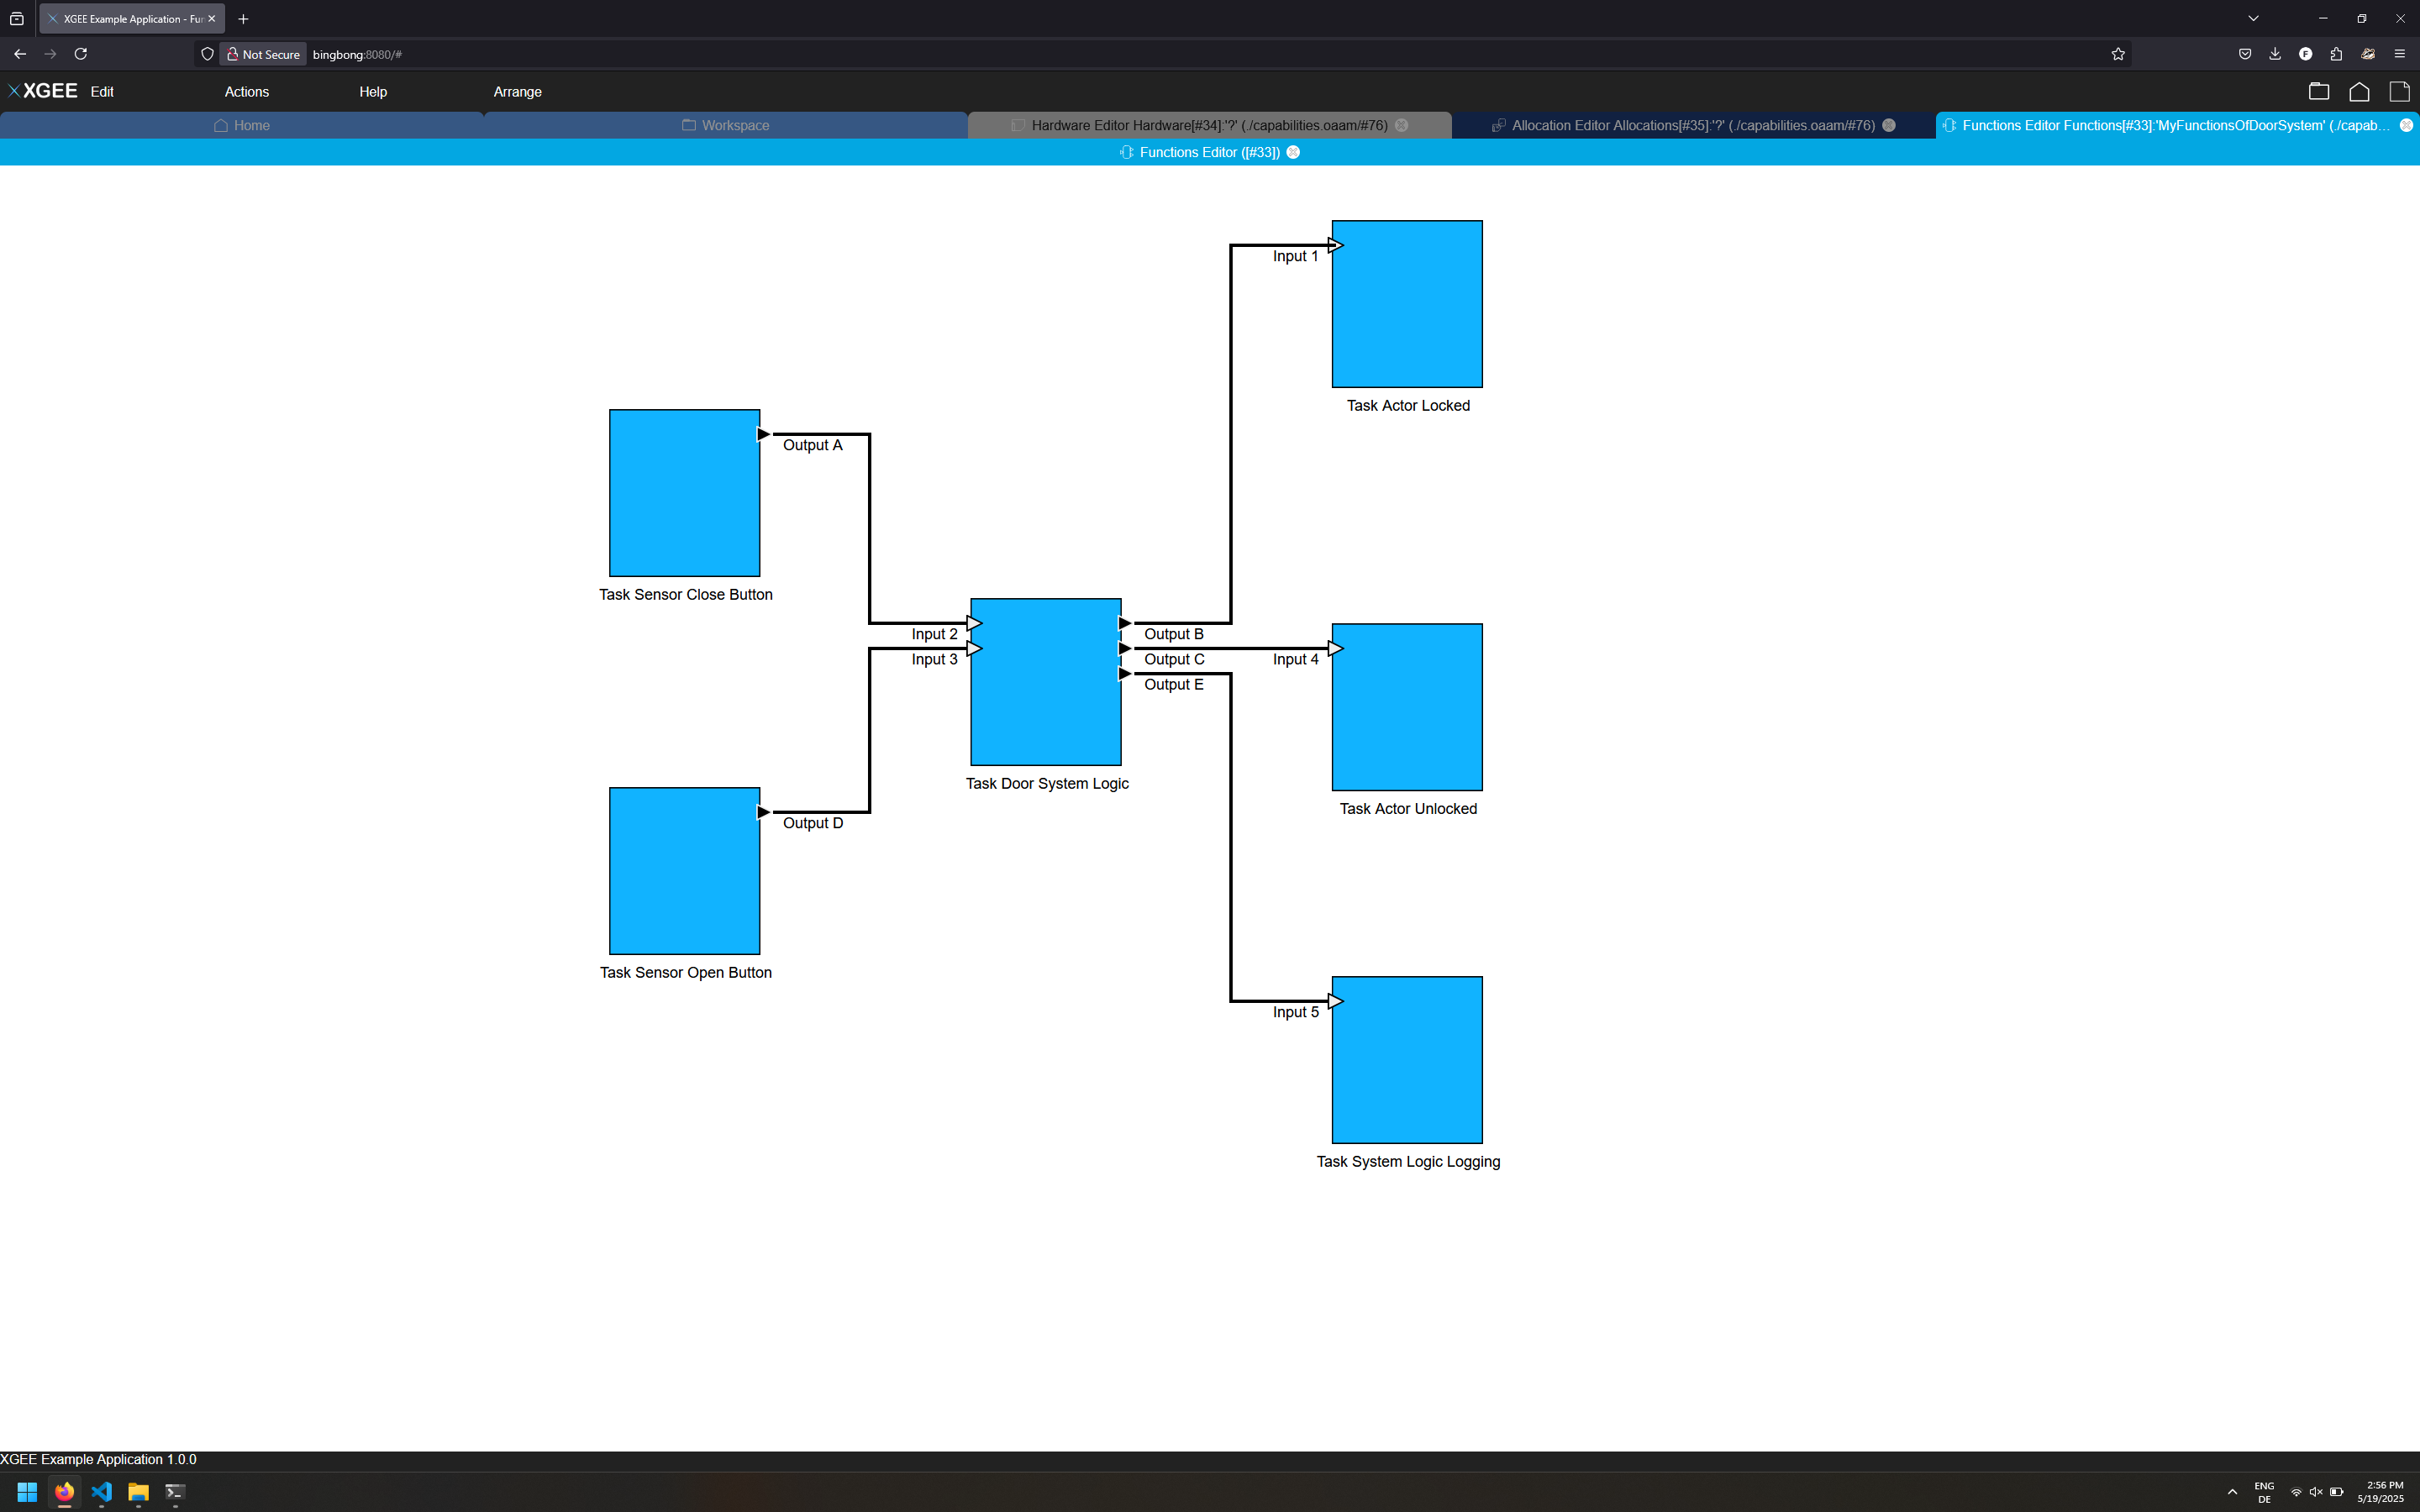
\includegraphics[width=\textwidth]{testcases/edge_10px_too_long/145613-303058_input_image.png}
        \caption*{\textit{Before}}
    \end{subfigure}
    \newline    
    \begin{subfigure}[t]{0.9\textwidth}
        \centering
        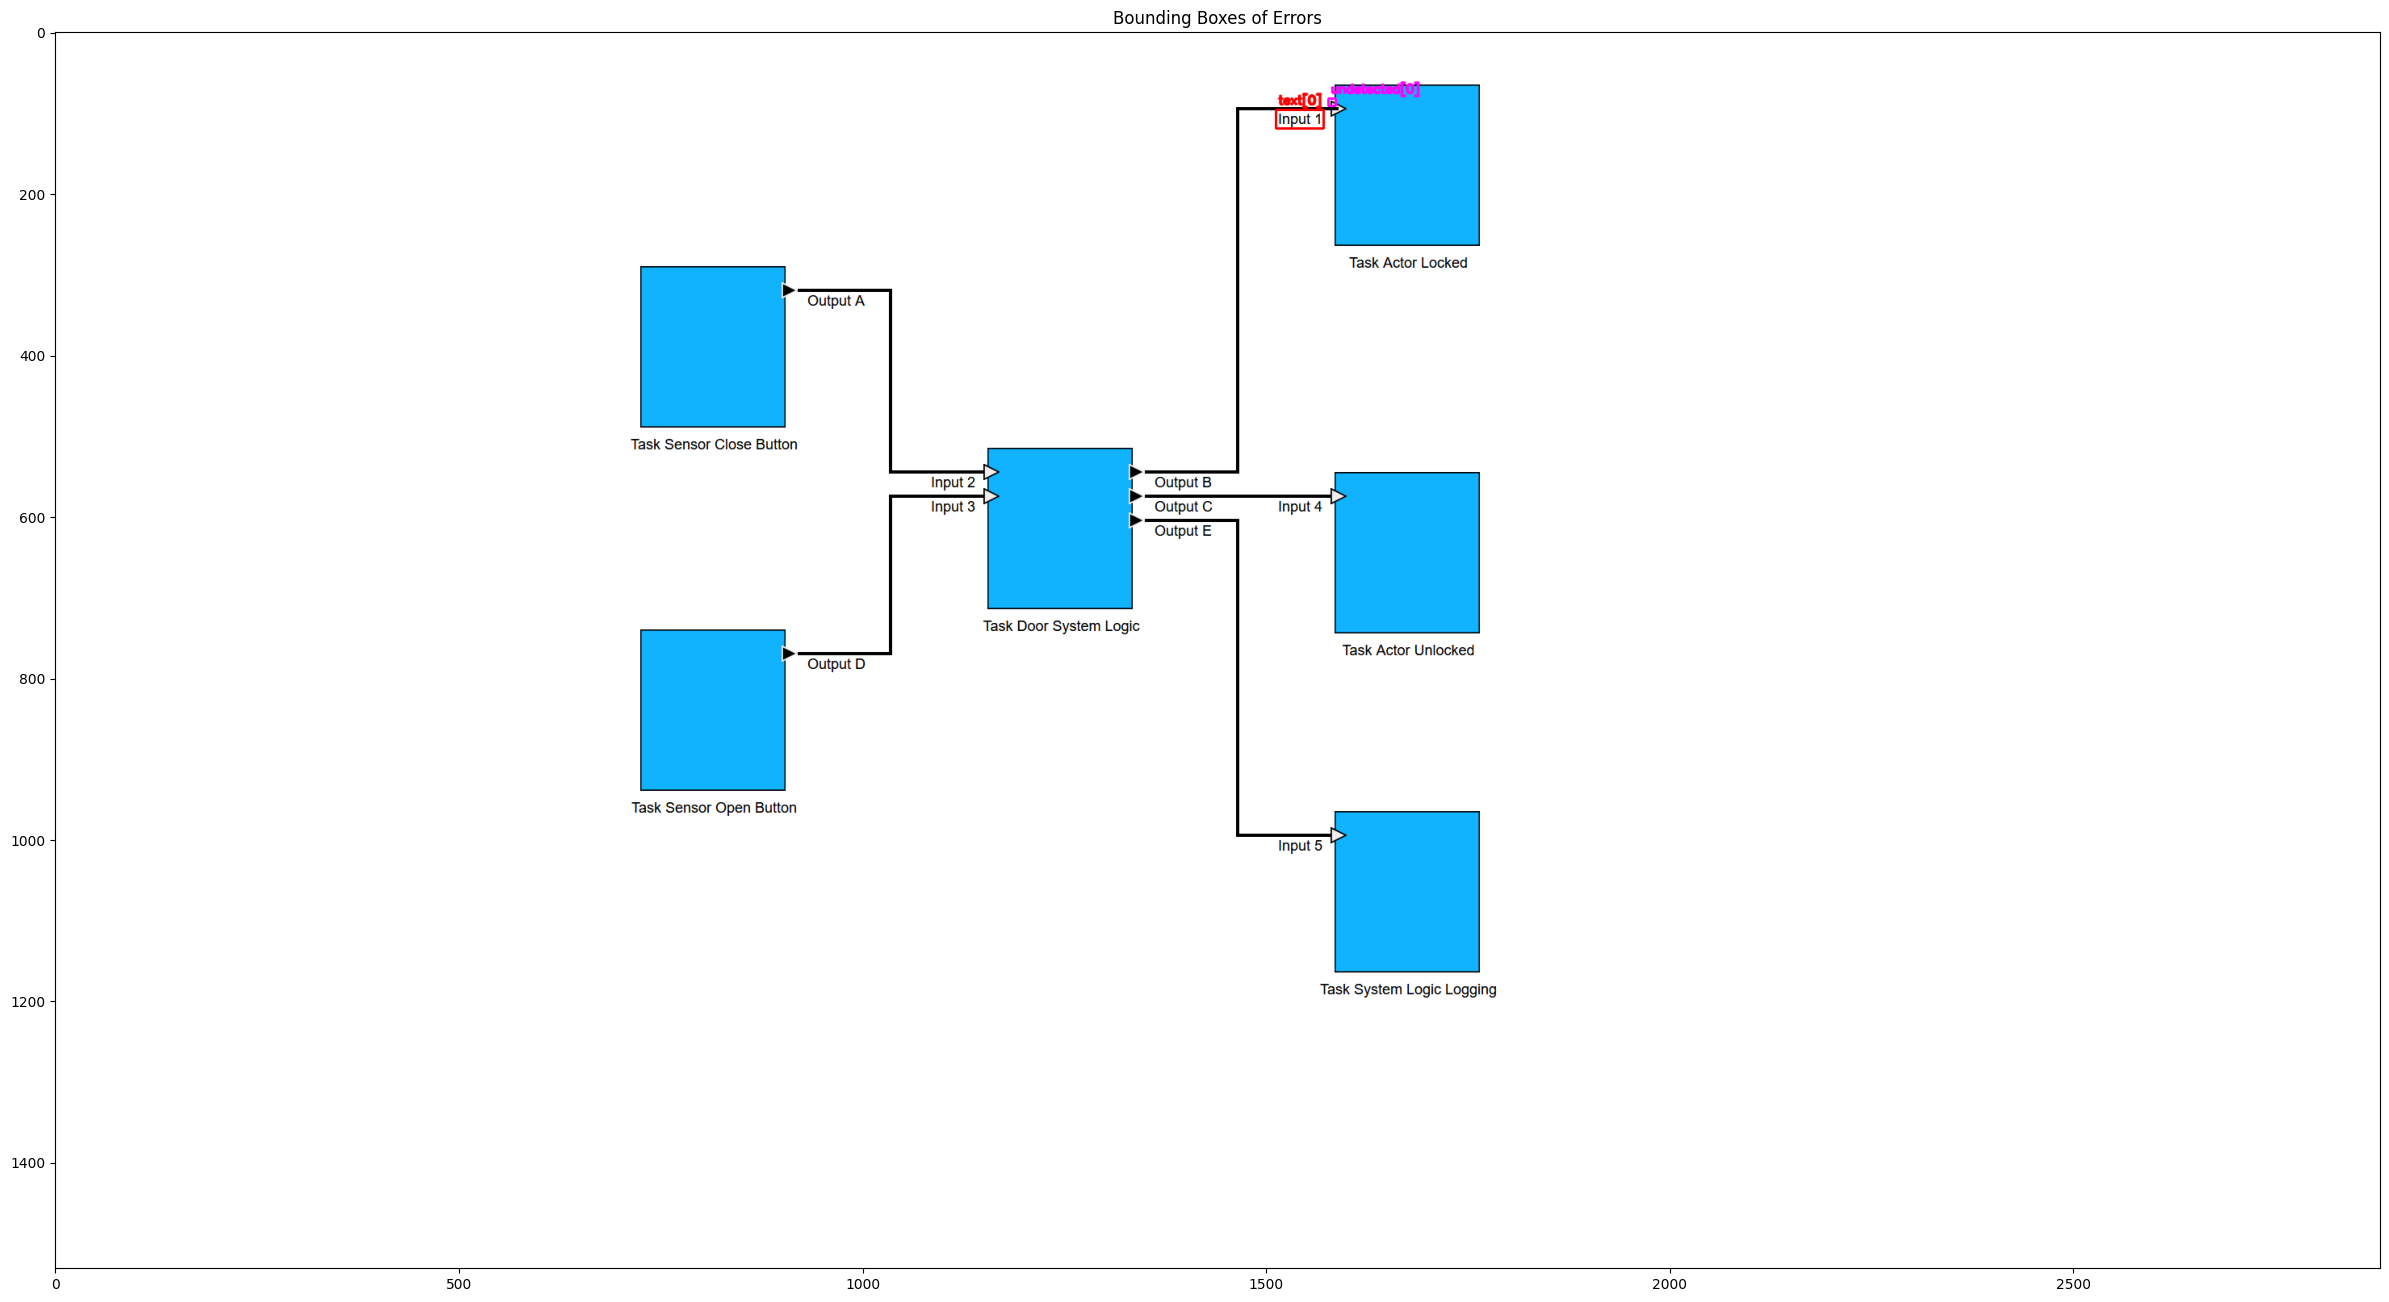
\includegraphics[width=\textwidth]{testcases/edge_10px_too_long/145632-779481_element_bbox_errors_labeled_colored.png}
        \caption*{\textit{After}}
    \end{subfigure}
    % \caption{Edge}
    \label{fig:edge_too_long_10}
\end{figure}
\newpage

\section{Edge 10px too short}
\begin{figure}[H]
    \centering
    \begin{subfigure}[t]{0.9\textwidth}
        \centering
        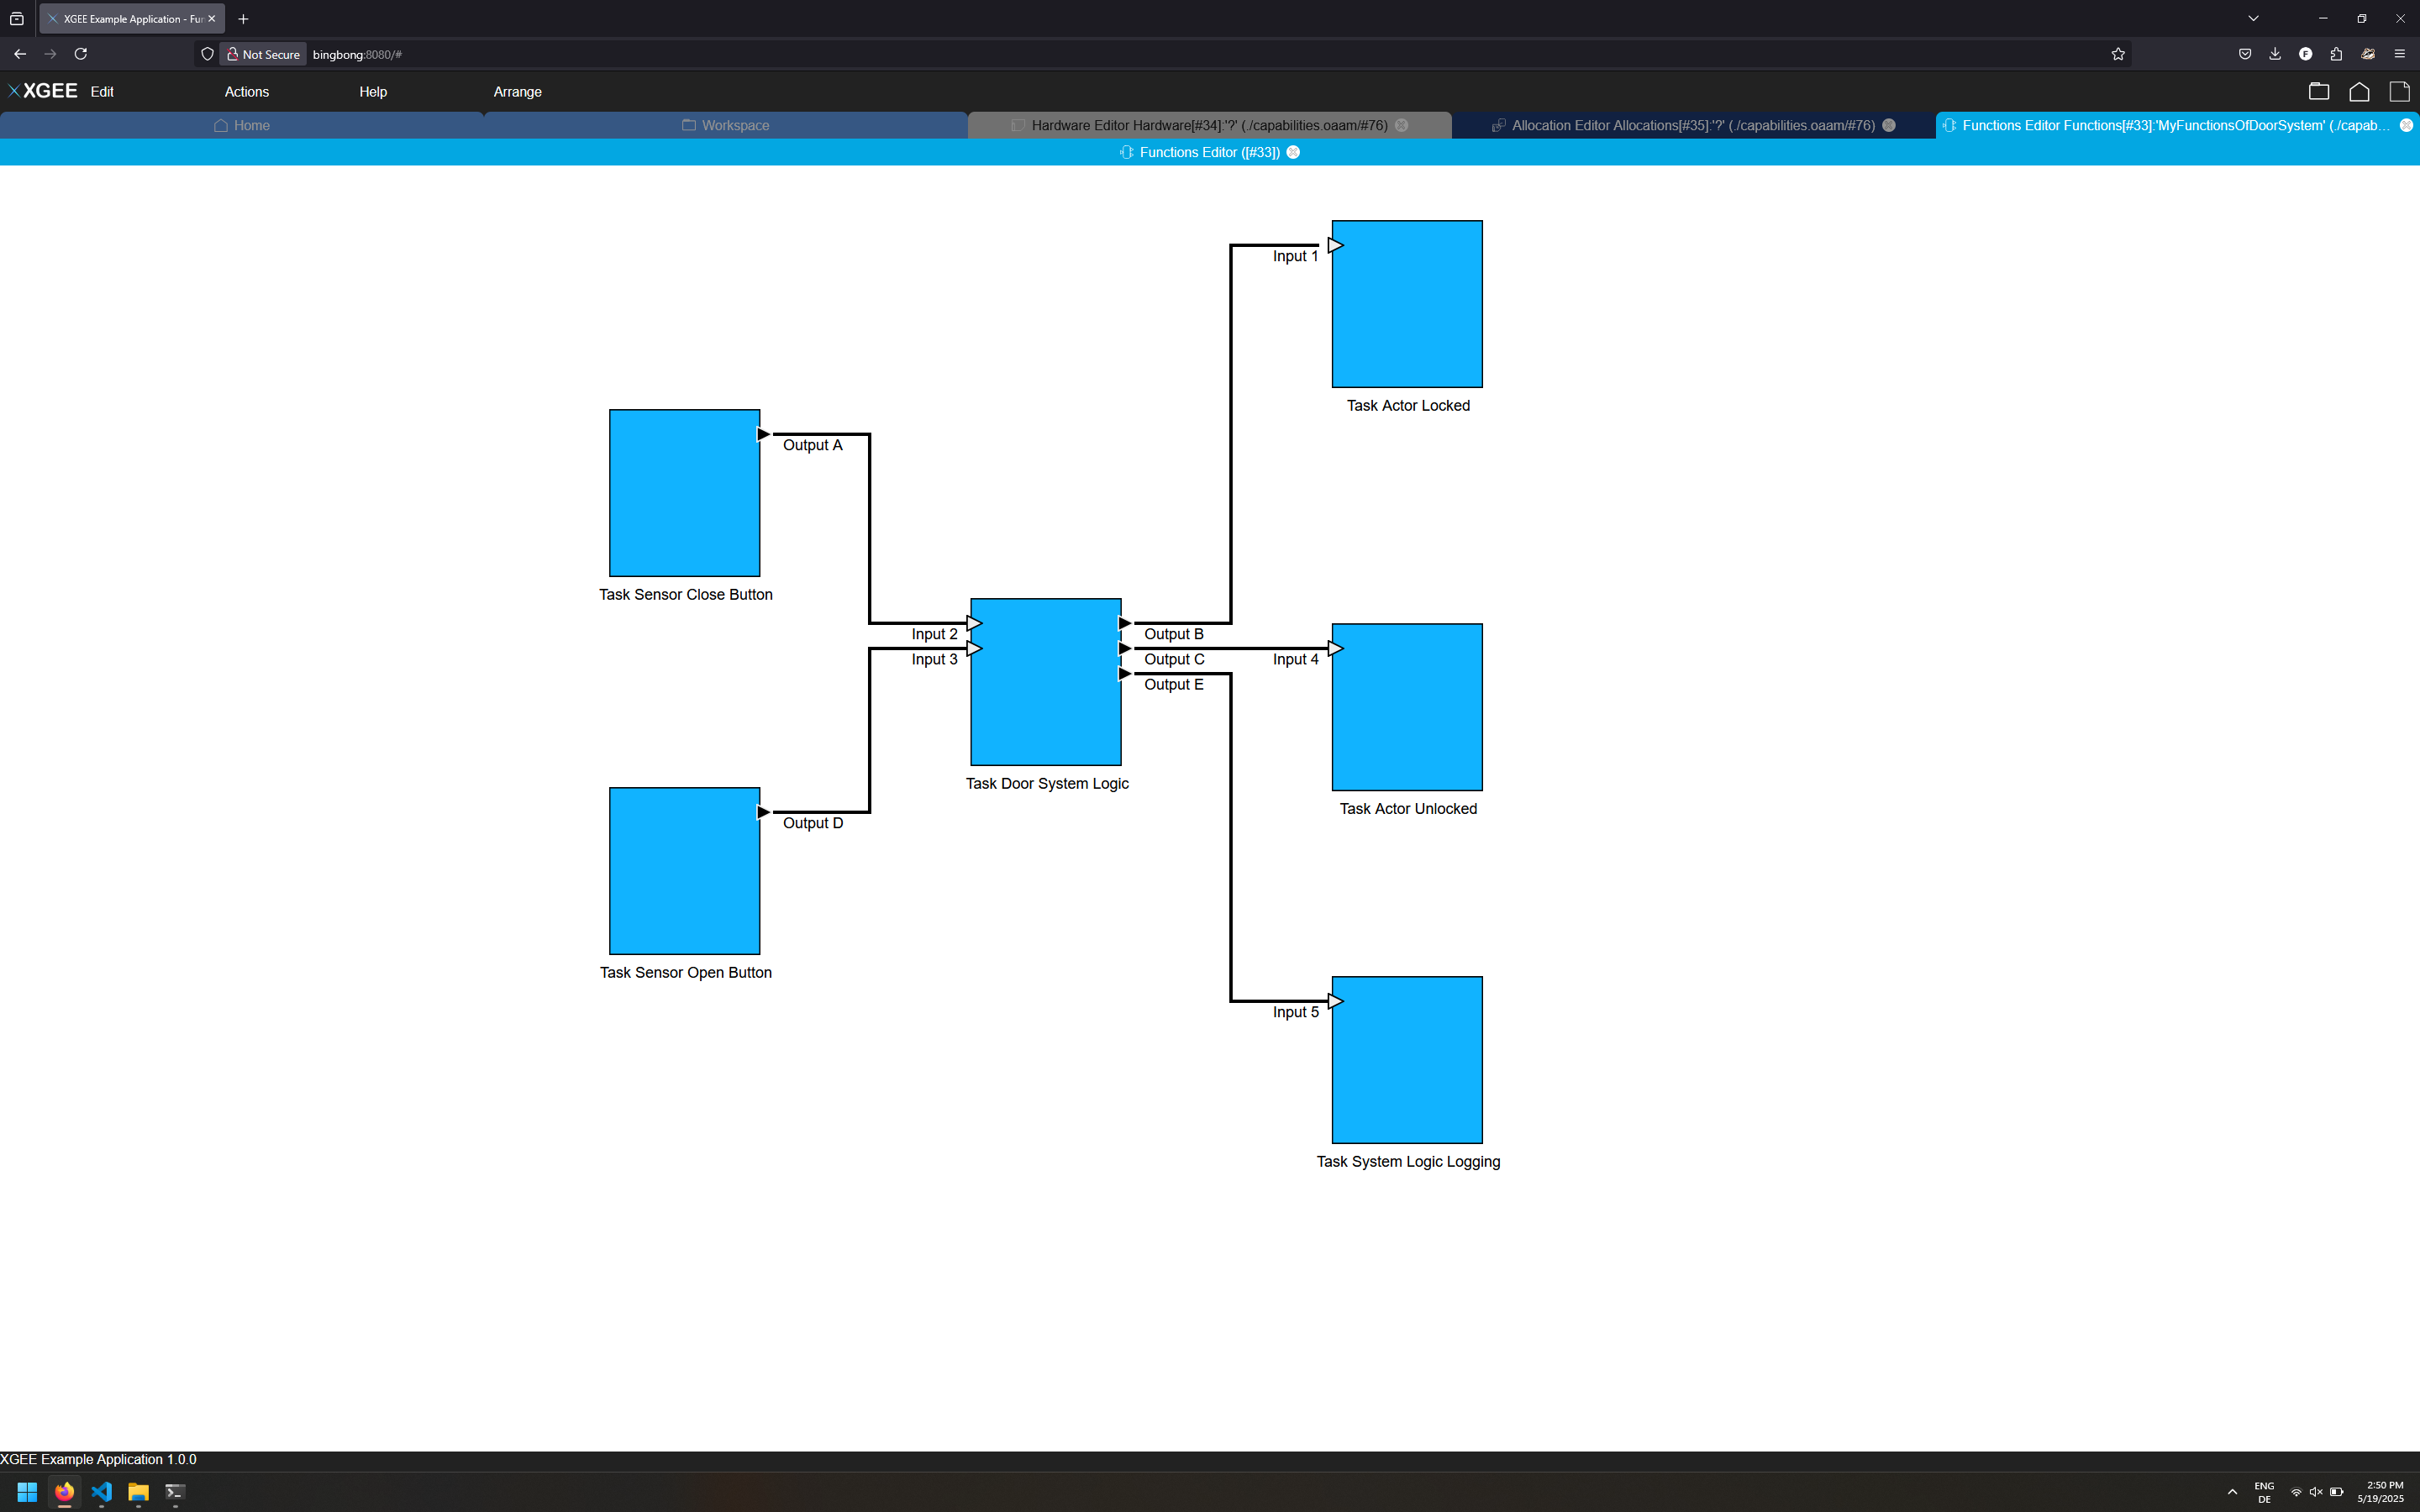
\includegraphics[width=\textwidth]{testcases/edge_10px_too_short/145039-079193_input_image.png}
        \caption*{\textit{Before}}
    \end{subfigure}
    \newline    
    \begin{subfigure}[t]{0.9\textwidth}
        \centering
        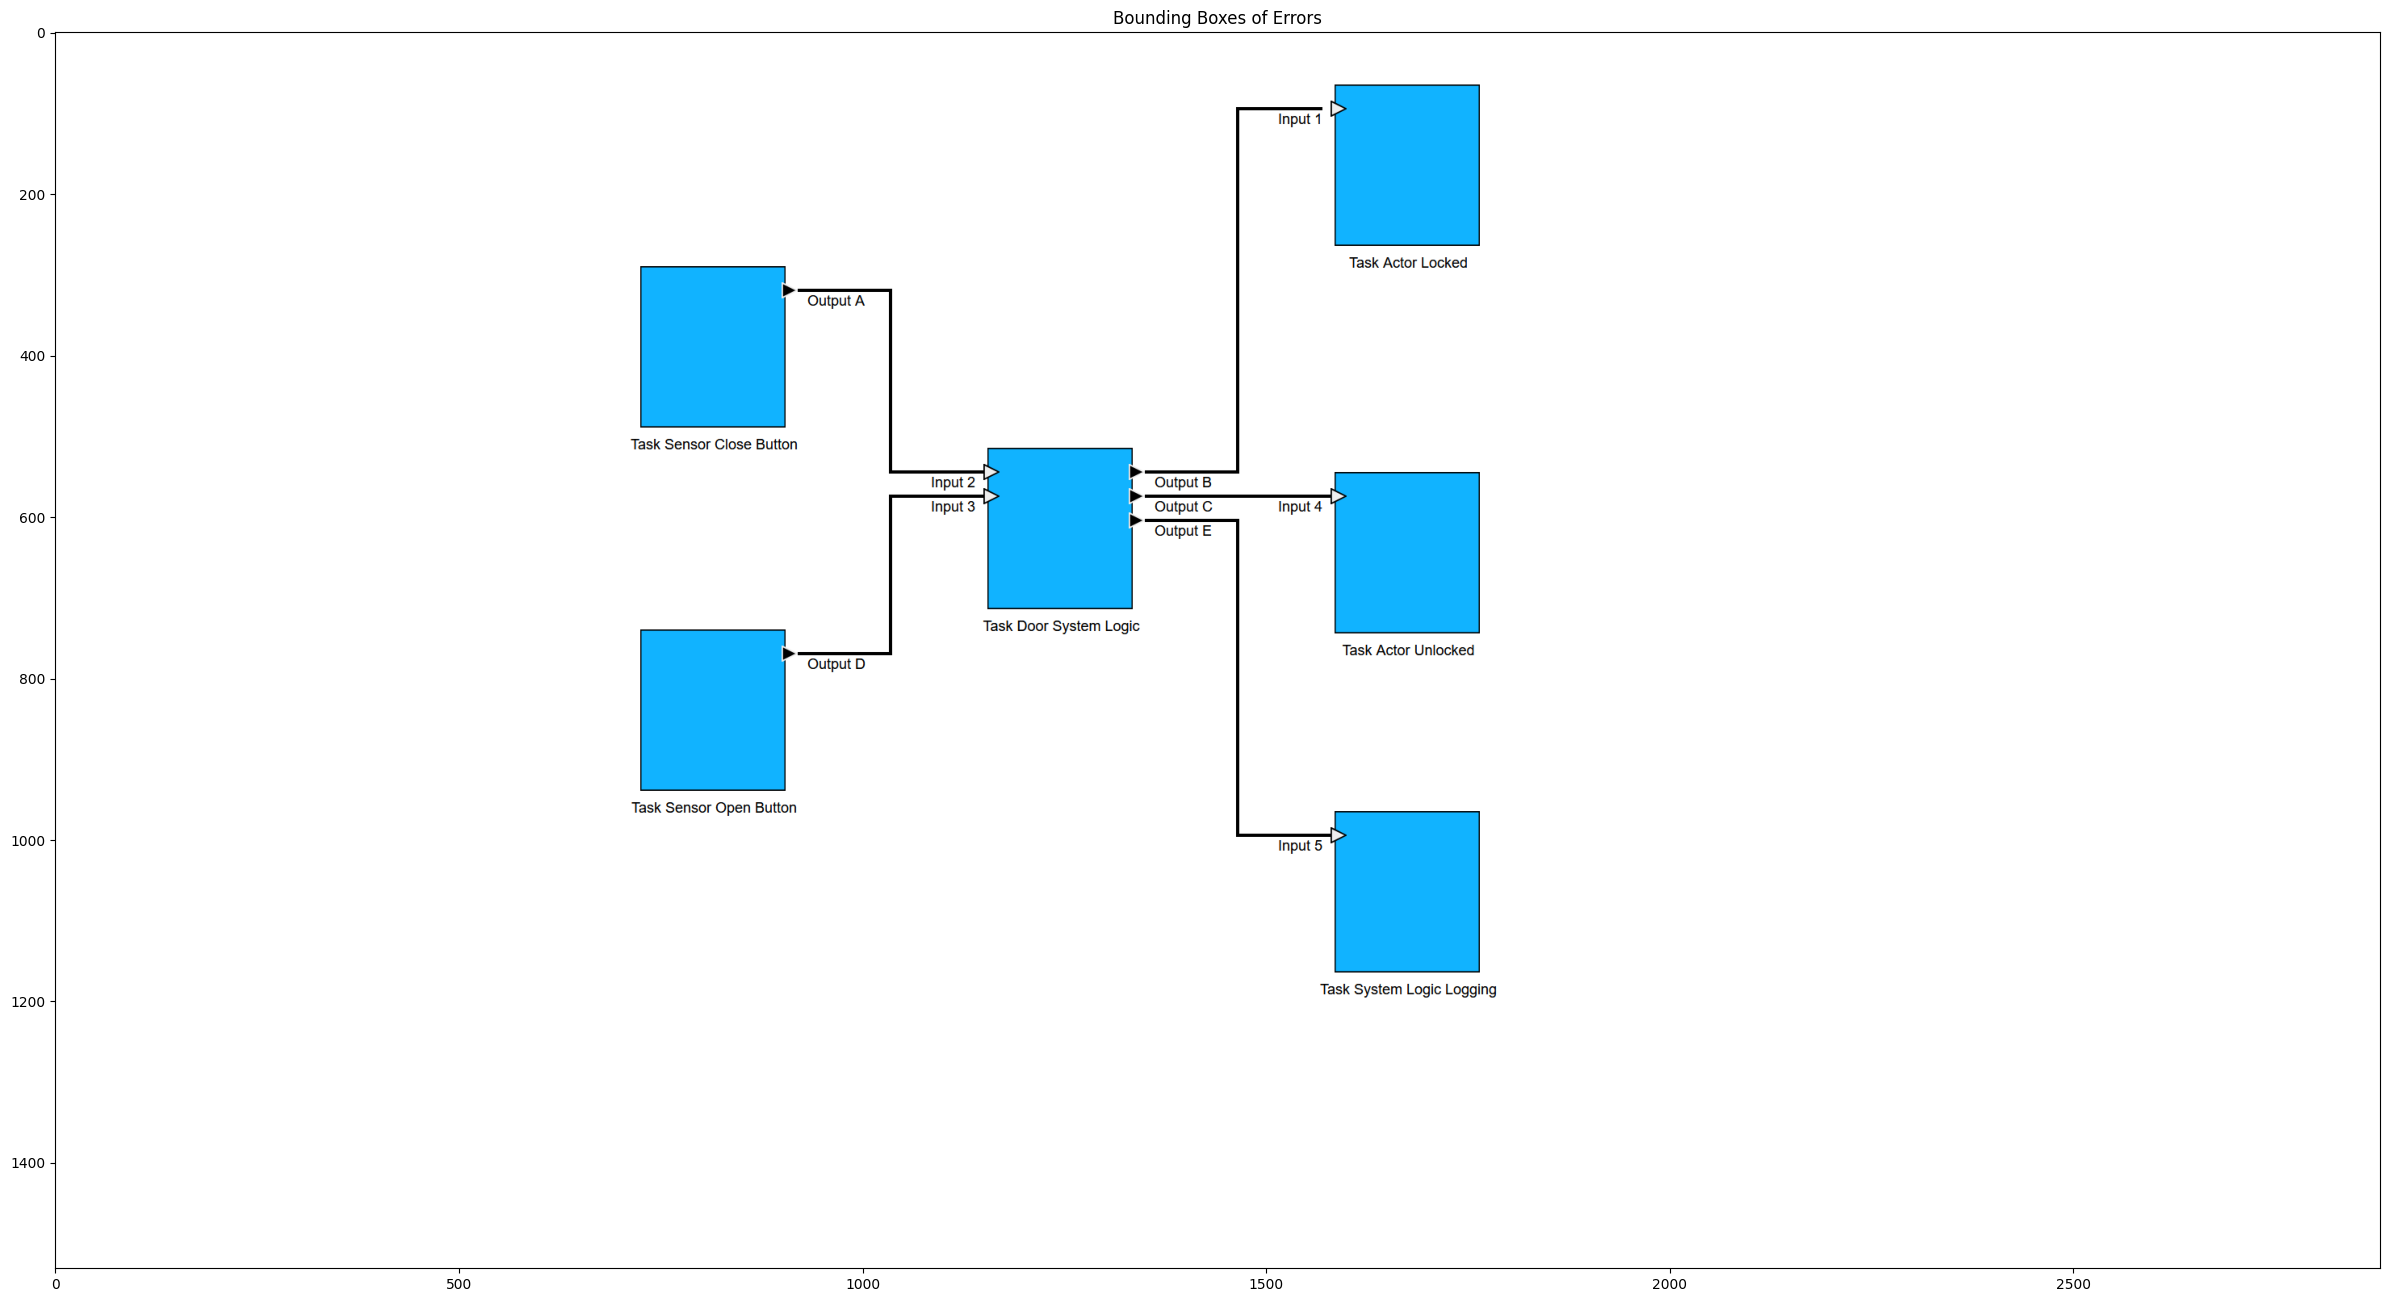
\includegraphics[width=\textwidth]{testcases/edge_10px_too_short/145058-578354_element_bbox_errors_labeled_colored.png}
        \caption*{\textit{After}}
    \end{subfigure}
    % \caption{Edge}
    \label{fig:edge_too_short_10}
\end{figure}
\newpage

\section{Edge 20px too short}
\begin{figure}[H]
    \centering
    \begin{subfigure}[t]{0.9\textwidth}
        \centering
        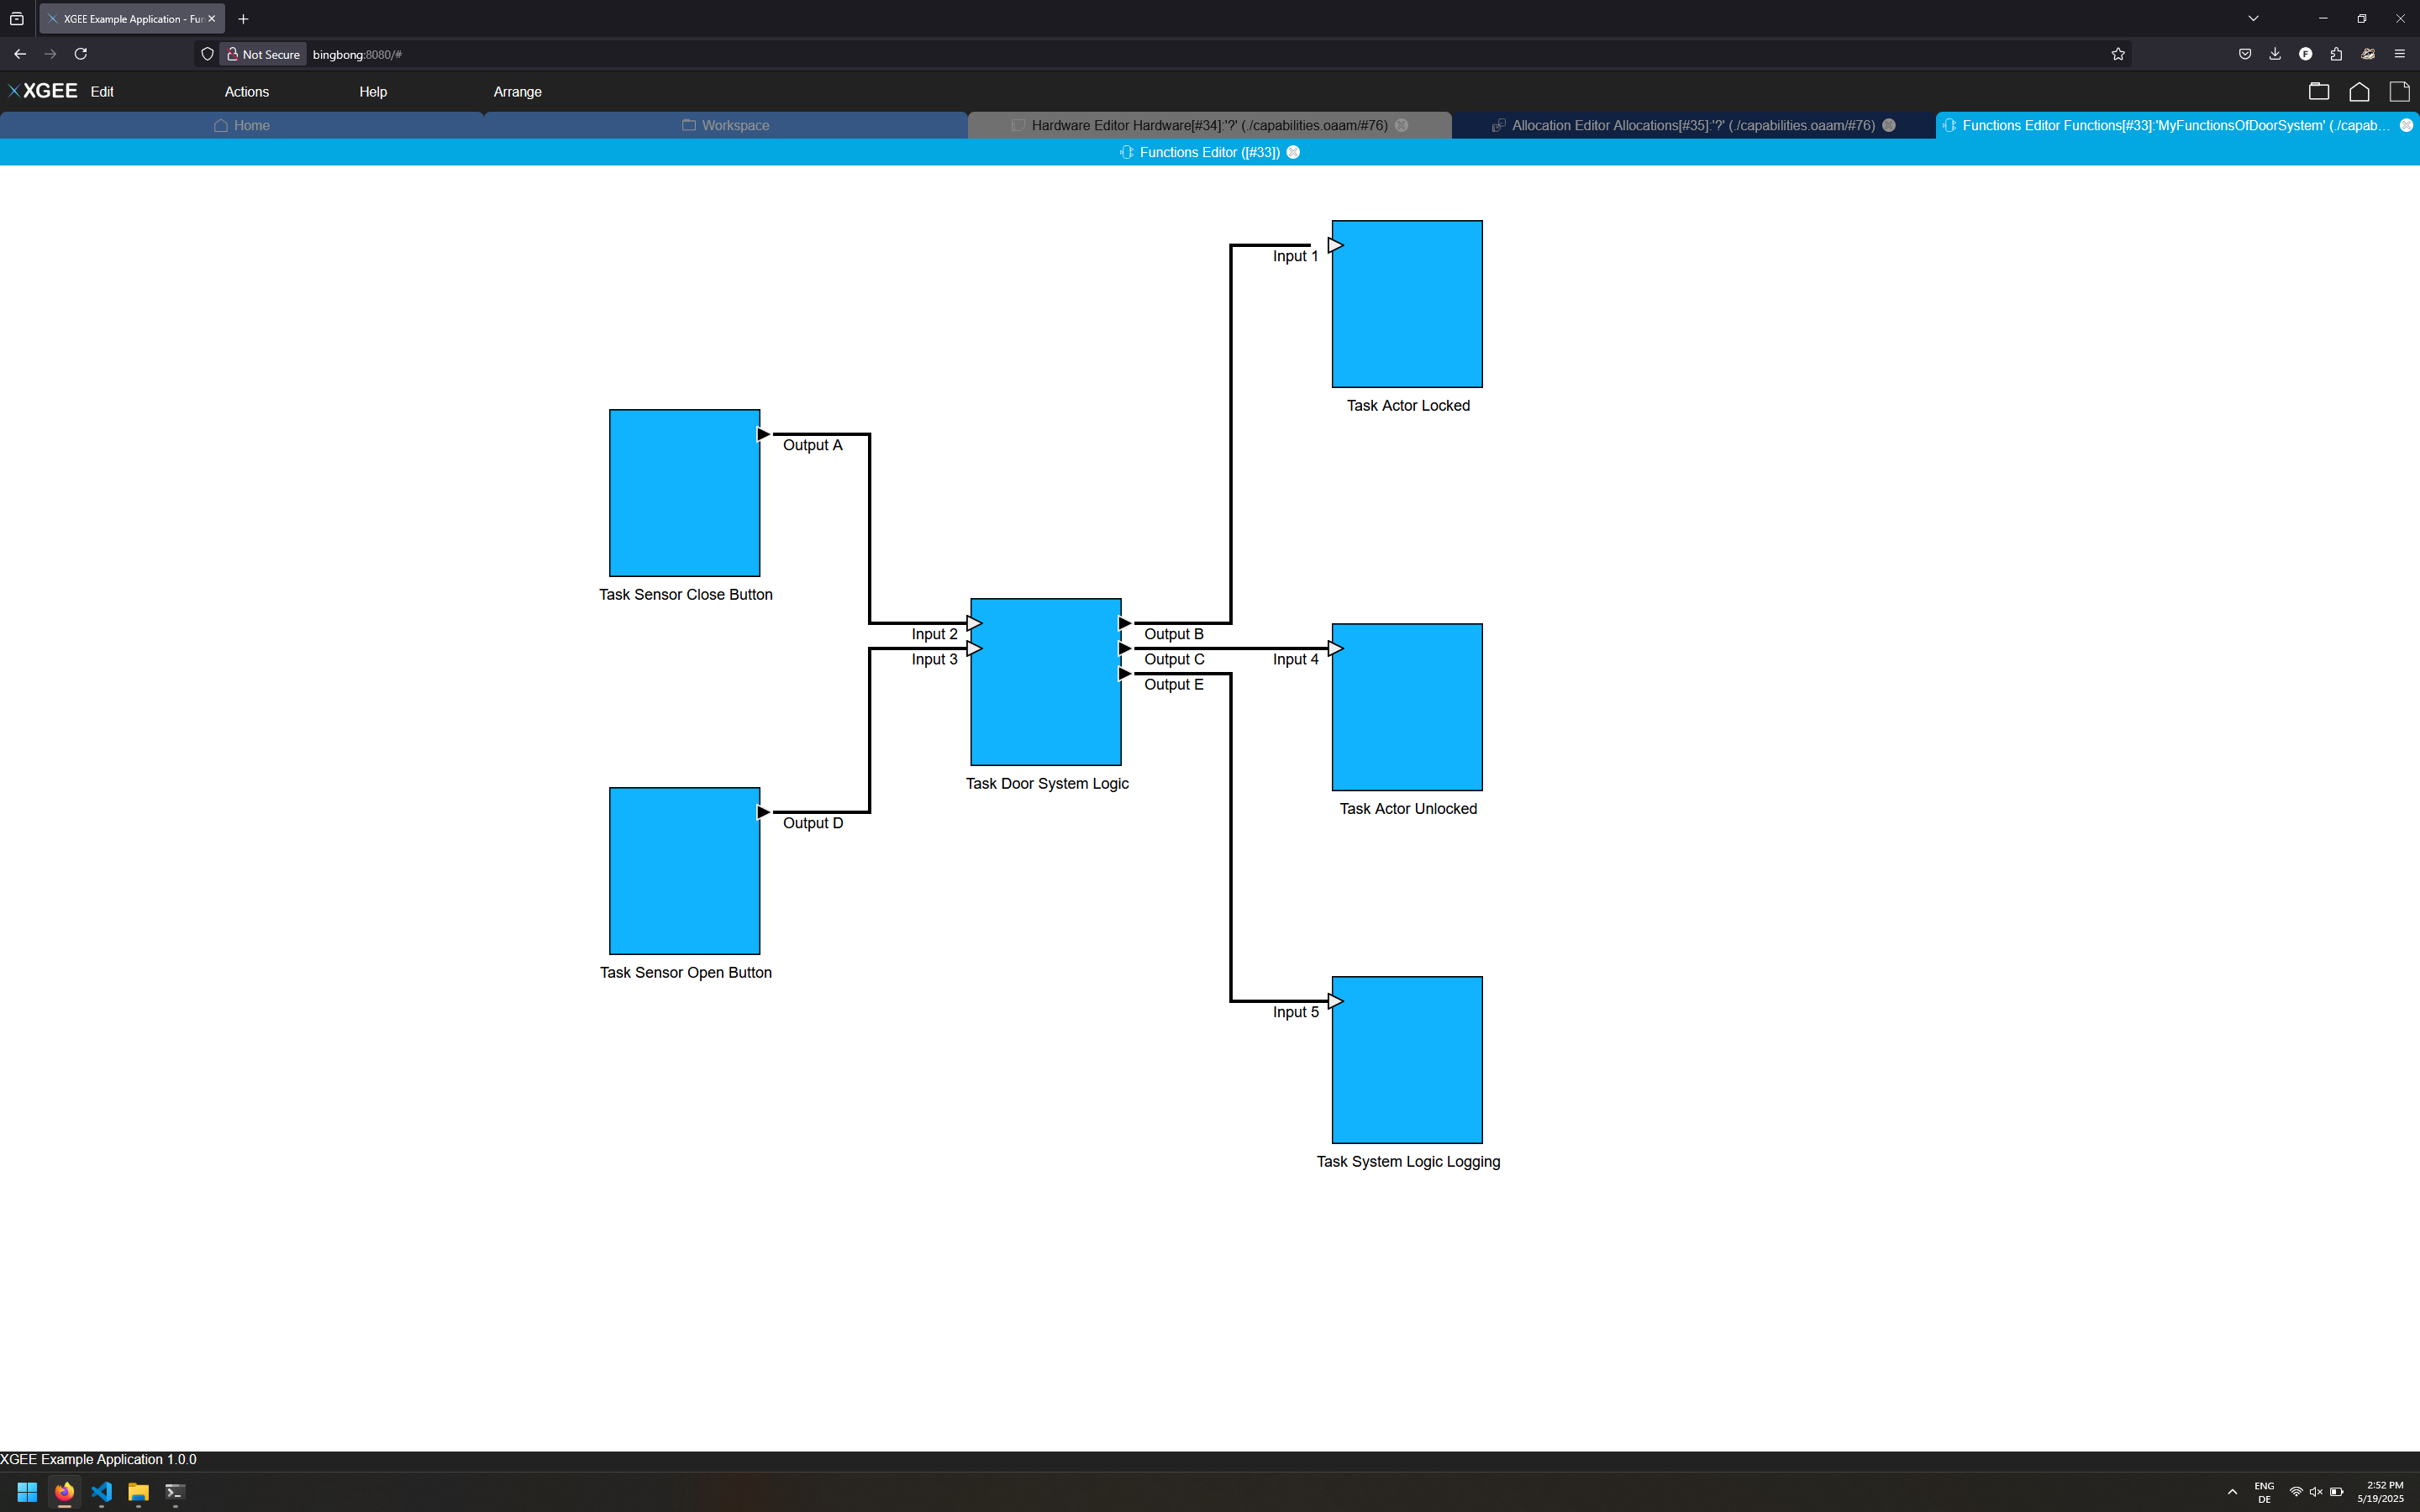
\includegraphics[width=\textwidth]{testcases/edge_20px_too_short/145244-393866_input_image.png}
        \caption*{\textit{Before}}
    \end{subfigure}
    \newline    
    \begin{subfigure}[t]{0.9\textwidth}
        \centering
        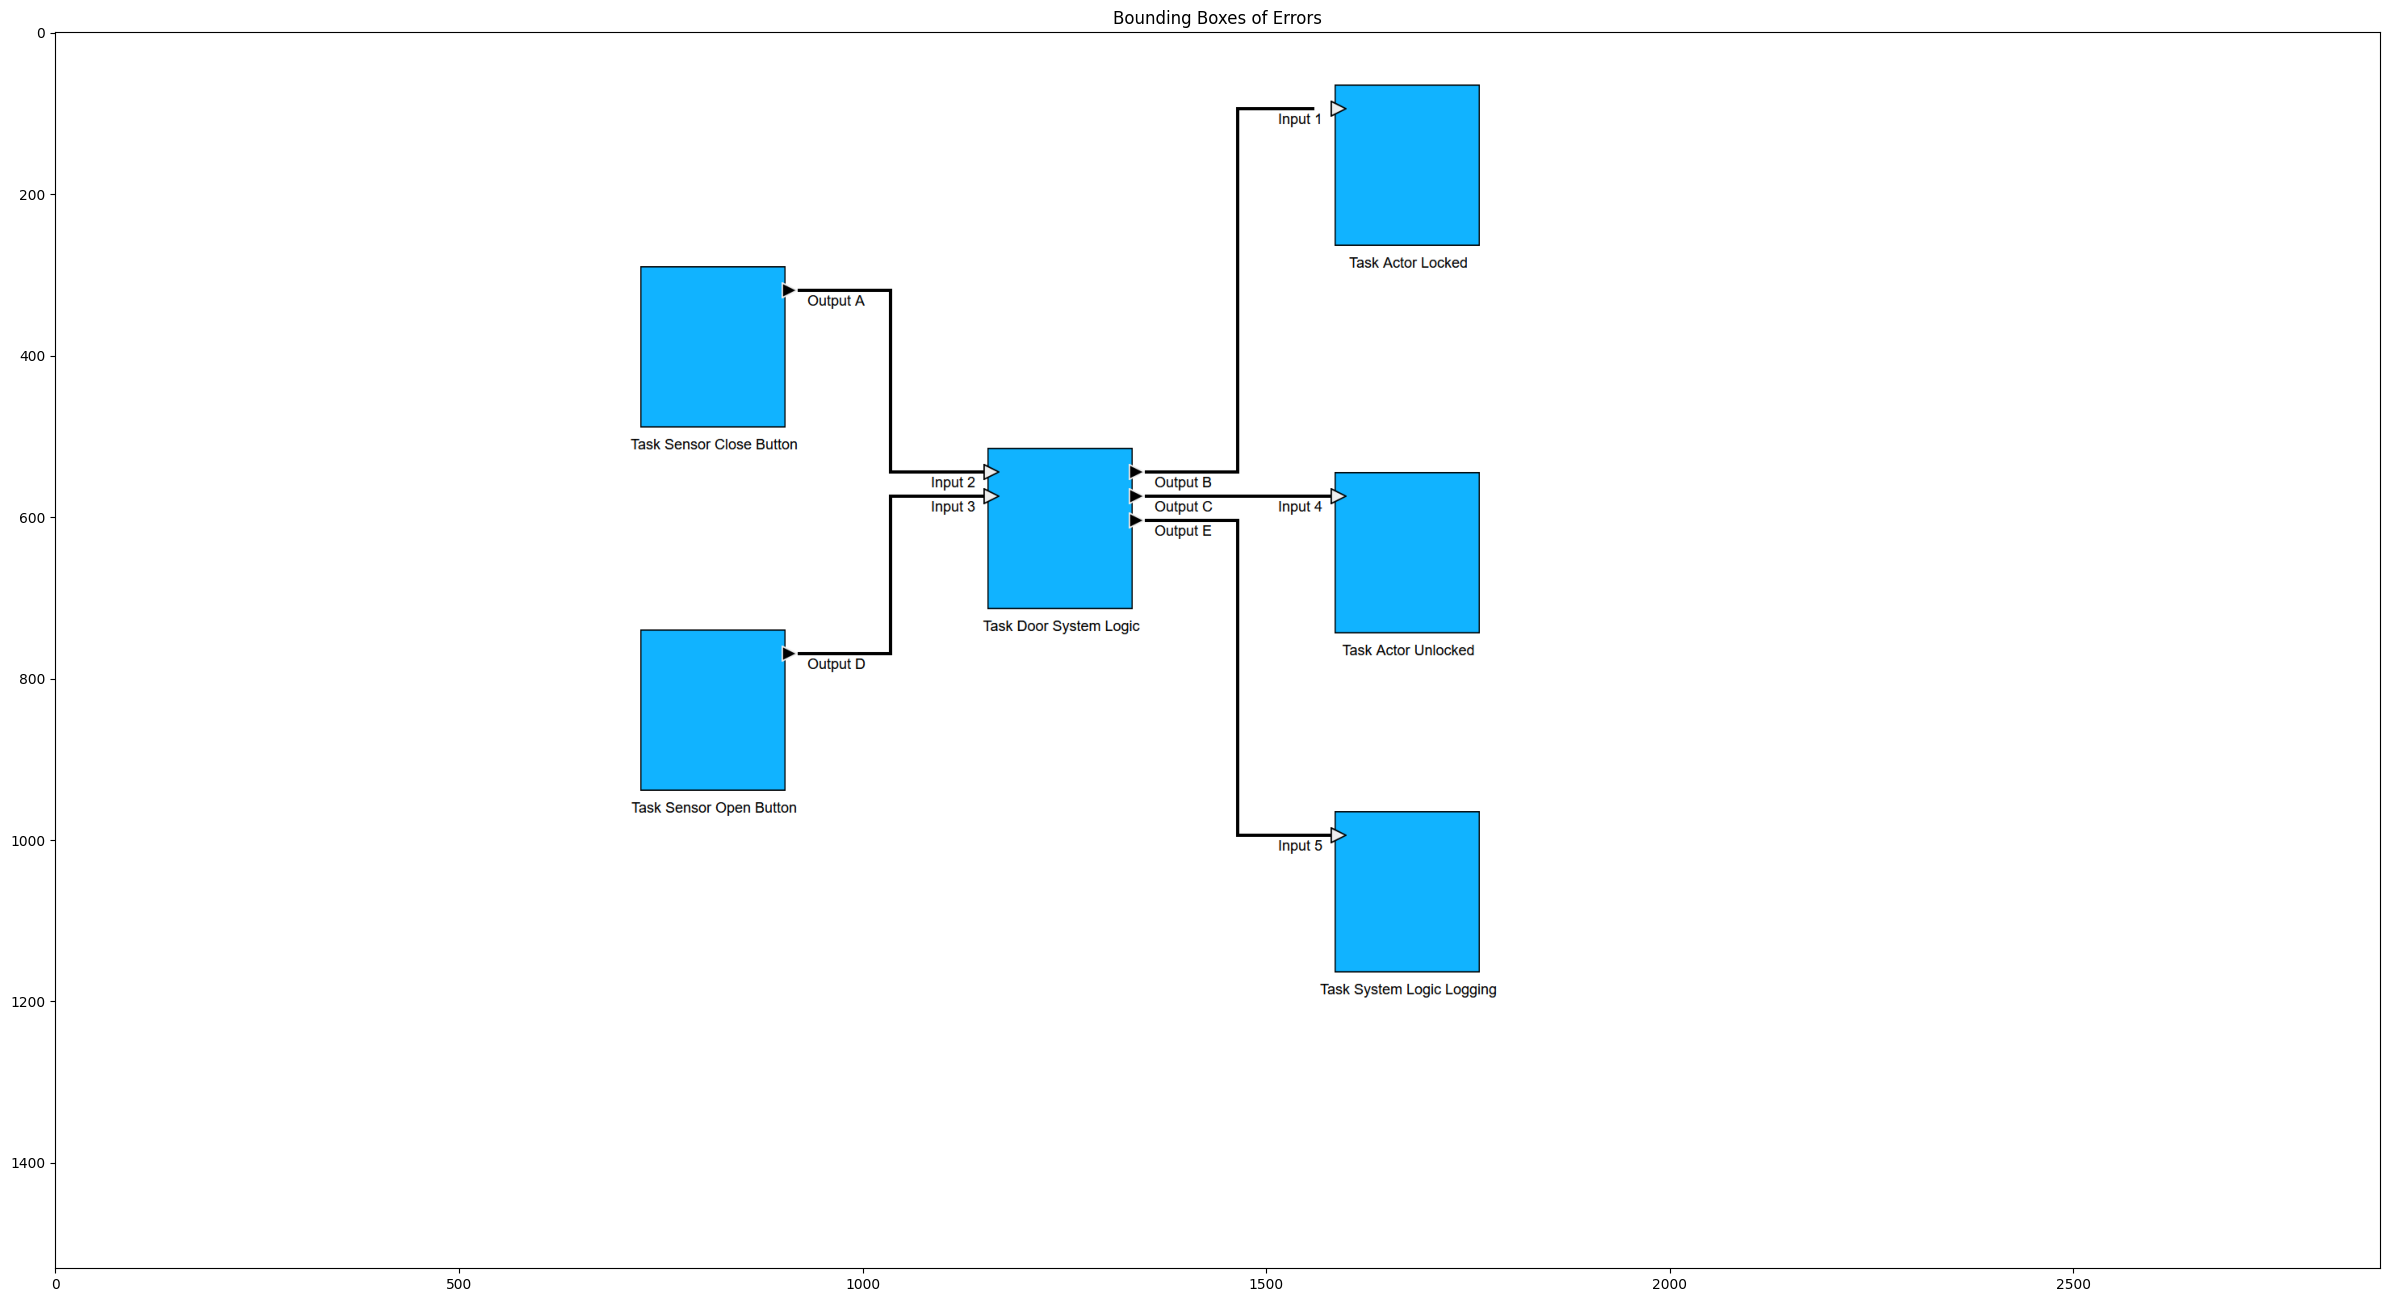
\includegraphics[width=\textwidth]{testcases/edge_20px_too_short/145304-754569_element_bbox_errors_labeled_colored.png}
        \caption*{\textit{After}}
    \end{subfigure}
    % \caption{Edge}
    \label{fig:edge_too_short_20}
\end{figure}
\newpage

\section{Edge connecting wrong elements}
\begin{figure}[H]
    \centering
    \begin{subfigure}[t]{0.9\textwidth}
        \centering
        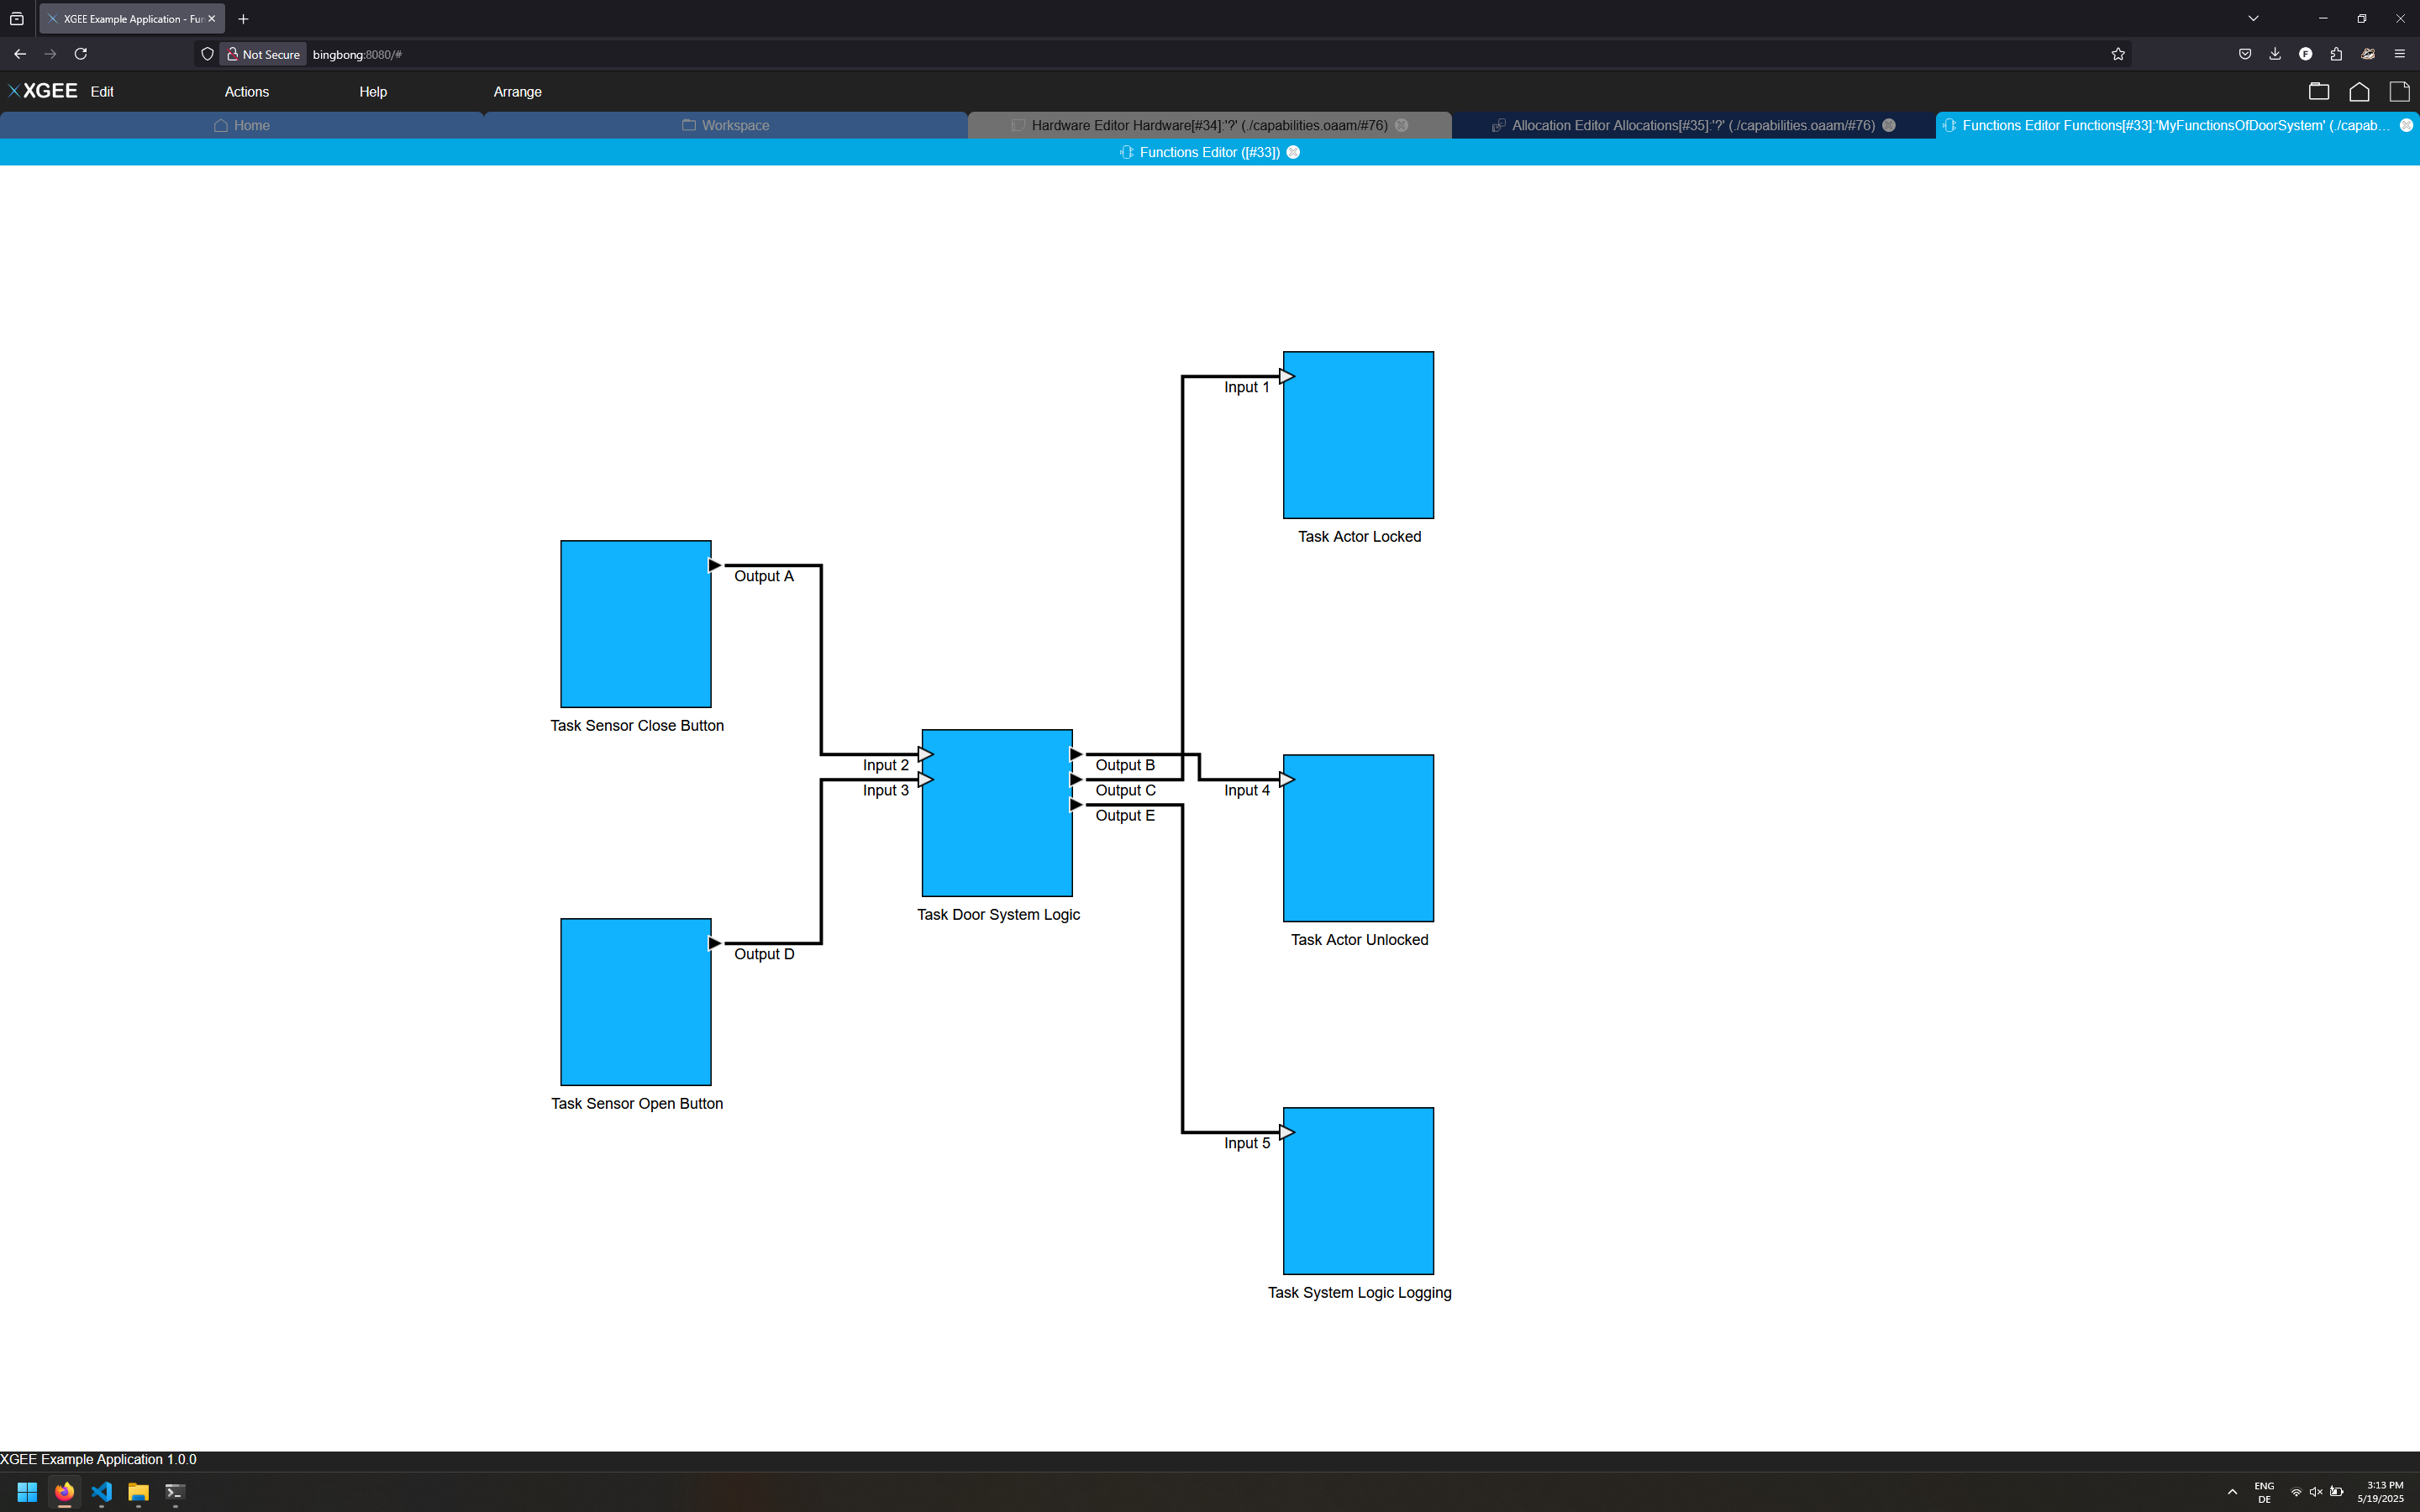
\includegraphics[width=\textwidth]{testcases/edge_connecting_wrong_elements/151304-831674_input_image.png}
        \caption*{\textit{Before}}
    \end{subfigure}
    \newline    
    \begin{subfigure}[t]{0.9\textwidth}
        \centering
        \includegraphics[width=\textwidth]{testcases/edge_connecting_wrong_elements/151317-638937_element_bbox_errors_labeled_colored.png}
        \caption*{\textit{After}}
    \end{subfigure}
    % \caption{Edge connecting wrong elements}
    \label{fig:edge_connecting_wrong}
\end{figure}
\newpage

\section{Edges too close to each other - 10px}
\begin{figure}[H]
    \centering
    \begin{subfigure}[t]{0.9\textwidth}
        \centering
        \includegraphics[width=\textwidth]{testcases/edge_too_close_10px_normal/151536-922393_input_image.png}
        \caption*{\textit{Before}}
    \end{subfigure}
    \newline    
    \begin{subfigure}[t]{0.9\textwidth}
        \centering
        \includegraphics[width=\textwidth]{testcases/edge_too_close_10px_normal/151548-984416_element_bbox_errors_labeled_colored.png}
        \caption*{\textit{After}}
    \end{subfigure}
    % \caption{Edges too close to each other}
    \label{fig:edges_too_close_10}
\end{figure}
\newpage

\section{Edges too close to each other - 5px}
\begin{figure}[H]
    \centering
    \begin{subfigure}[t]{0.9\textwidth}
        \centering
        \includegraphics[width=\textwidth]{testcases/edge_too_close_5px_assisted/151733-188571_input_image.png}
        \caption*{\textit{Before}}
    \end{subfigure}
    \newline    
    \begin{subfigure}[t]{0.9\textwidth}
        \centering
        \includegraphics[width=\textwidth]{testcases/edge_too_close_5px_assisted/151745-239534_element_bbox_errors_labeled_colored.png}
        \caption*{\textit{After}}
    \end{subfigure}
    % \caption{Edges too close to each other}
    \label{fig:edges_too_close_5}
\end{figure}
\newpage

\section{Edges forming ambiguous intersections}
\begin{figure}[H]
    \centering
    \begin{subfigure}[t]{0.9\textwidth}
        \centering
        \includegraphics[width=\textwidth]{testcases/edges_forming_bad_intersection/151929-204247_input_image.png}
        \caption*{\textit{Before}}
    \end{subfigure}
    \newline    
    \begin{subfigure}[t]{0.9\textwidth}
        \centering
        \includegraphics[width=\textwidth]{testcases/edges_forming_bad_intersection/151941-652255_element_bbox_errors_labeled_colored.png}
        \caption*{\textit{After}}
    \end{subfigure}
    % \caption{Edges forming ambiguous intersections}
    \label{fig:edges_ambiguous_intersections}
\end{figure}
\newpage

\section{Edges partly offscreen}
\begin{figure}[H]
    \centering
    \begin{subfigure}[t]{0.9\textwidth}
        \centering
        \includegraphics[width=\textwidth]{testcases/edge_offscreen_partly/152242-895612_input_image.png}
        \caption*{\textit{Before}}
    \end{subfigure}
    \newline    
    \begin{subfigure}[t]{0.9\textwidth}
        \centering
        \includegraphics[width=\textwidth]{testcases/edge_offscreen_partly/152255-292353_element_bbox_errors_labeled_colored.png}
        \caption*{\textit{After}}
    \end{subfigure}
    % \caption{Edges offscreen}
    \label{fig:edges_partly_offscreen}
\end{figure}
\newpage

\section{Edges completly offscreen}
\begin{figure}[H]
    \centering
    \begin{subfigure}[t]{0.9\textwidth}
        \centering
        \includegraphics[width=\textwidth]{testcases/edge_offscreen_completely/152114-079741_input_image.png}
        \caption*{\textit{Before}}
    \end{subfigure}
    \newline    
    \begin{subfigure}[t]{0.9\textwidth}
        \centering
        \includegraphics[width=\textwidth]{testcases/edge_offscreen_completely/152126-889602_element_bbox_errors_labeled_colored.png}
        \caption*{\textit{After}}
    \end{subfigure}
    % \caption{Edges offscreen}
    \label{fig:edges_completly_offscreen}
\end{figure}
\newpage

\section{Edge in visualization, but not in model}

\newpage

\section{Edge in model, but not in visualization}
\begin{figure}[H]
    \centering
    \begin{subfigure}[t]{0.9\textwidth}
        \centering
        \includegraphics[width=\textwidth]{testcases/edge_in_model_not_in_visualization/152413-910376_input_image.png}
        \caption*{\textit{Before}}
    \end{subfigure}
    \newline    
    \begin{subfigure}[t]{0.9\textwidth}
        \centering
        \includegraphics[width=\textwidth]{testcases/edge_in_model_not_in_visualization/152427-029742_element_bbox_errors_labeled_colored.png}
        \caption*{\textit{After}}
    \end{subfigure}
    % \caption{Edge in model, but not in visualization}
    \label{fig:edge_in_model_not_viz}
\end{figure}
\newpage

% ------------------------
% Text Issues
% ------------------------

\section{Text 5pt too small}
\begin{figure}[H]
    \centering
    \begin{subfigure}[t]{0.9\textwidth}
        \centering
        \includegraphics[width=\textwidth]{testcases/text_5pt_too_small/154310-836128_input_image.png}
        \caption*{\textit{Before}}
    \end{subfigure}
    \newline
    \begin{subfigure}[t]{0.9\textwidth}
        \centering
        \includegraphics[width=\textwidth]{testcases/text_5pt_too_small/154323-370828_element_bbox_errors_labeled_colored.png}
        \caption*{\textit{After}}
    \end{subfigure}
    % \caption{Text too small}
    \label{fig:text_too_small_5}
\end{figure}
\newpage

\section{Text 10pt too small}
\begin{figure}[H]
    \centering
    \begin{subfigure}[t]{0.9\textwidth}
        \centering
        \includegraphics[width=\textwidth]{testcases/text_10pt_too_small/154344-435789_input_image.png}
        \caption*{\textit{Before}}
    \end{subfigure}
    \newline
    \begin{subfigure}[t]{0.9\textwidth}
        \centering
        \includegraphics[width=\textwidth]{testcases/text_10pt_too_small/154357-030783_element_bbox_errors_labeled_colored.png}
        \caption*{\textit{After}}
    \end{subfigure}
    % \caption{Text too small}
    \label{fig:text_too_small_10}
\end{figure}
\newpage

\section{Text 5pt too large}
\begin{figure}[H]
    \centering
    \begin{subfigure}[t]{0.9\textwidth}
        \centering
        \includegraphics[width=\textwidth]{testcases/text_5pt_too_large/154503-258136_input_image.png}
        \caption*{\textit{Before}}
    \end{subfigure}
    \newline
    \begin{subfigure}[t]{0.9\textwidth}
        \centering
        \includegraphics[width=\textwidth]{testcases/text_5pt_too_large/154516-359589_element_bbox_errors_labeled_colored.png}
        \caption*{\textit{After}}
    \end{subfigure}
    % \caption{Text too large}
    \label{fig:text_too_large_5}
\end{figure}
\newpage

\section{Text 10pt too large}
\begin{figure}[H]
    \centering
    \begin{subfigure}[t]{0.9\textwidth}
        \centering
        \includegraphics[width=\textwidth]{testcases/text_10pt_too_large/154559-088336_input_image.png}
        \caption*{\textit{Before}}
    \end{subfigure}
    \newline
    \begin{subfigure}[t]{0.9\textwidth}
        \centering
        \includegraphics[width=\textwidth]{testcases/text_10pt_too_large/154611-579883_element_bbox_errors_labeled_colored.png}
        \caption*{\textit{After}}
    \end{subfigure}
    % \caption{Text too large}
    \label{fig:text_too_large_10}
\end{figure}
\newpage

\section{Text wrong in visualization}
\begin{figure}[H]
    \centering
    \begin{subfigure}[t]{0.9\textwidth}
        \centering
        \includegraphics[width=\textwidth]{testcases/text_wrong_in_visualization/160949-255974_input_image.png}
        \caption*{\textit{Before}}
    \end{subfigure}
    \newline
    \begin{subfigure}[t]{0.9\textwidth}
        \centering
        \includegraphics[width=\textwidth]{testcases/text_wrong_in_visualization/161009-586327_element_bbox_errors_labeled_colored.png}
        \caption*{\textit{After}}
    \end{subfigure}
    % \caption{Text wrong color}
    \label{fig:text_wrong_in_viz}
\end{figure}
\newpage

\section{Text wrong color}
\begin{figure}[H]
    \centering
    \begin{subfigure}[t]{0.9\textwidth}
        \centering
        \includegraphics[width=\textwidth]{testcases/text_wrong_color/155122-094397_input_image.png}
        \caption*{\textit{Before}}
    \end{subfigure}
    \newline
    \begin{subfigure}[t]{0.9\textwidth}
        \centering
        \includegraphics[width=\textwidth]{testcases/text_wrong_color/155134-981060_element_bbox_errors_labeled_colored.png}
        \caption*{\textit{After}}
    \end{subfigure}
    % \caption{Text wrong color}
    \label{fig:text_wrong_color}
\end{figure}
\newpage

\section{Text 10px too low}
\begin{figure}[H]
    \centering
    \begin{subfigure}[t]{0.9\textwidth}
        \centering
        \includegraphics[width=\textwidth]{testcases/text_10px_too_low/155426-766429_input_image.png}
        \caption*{\textit{Before}}
    \end{subfigure}
    \newline
    \begin{subfigure}[t]{0.9\textwidth}
        \centering
        \includegraphics[width=\textwidth]{testcases/text_10px_too_low/155439-414936_element_bbox_errors_labeled_colored.png}
        \caption*{\textit{After}}
    \end{subfigure}
    % \caption{Text in wrong position relative to parent element}
    \label{fig:text_too_low_10}
\end{figure}
\newpage

\section{Text 10px too high}
\begin{figure}[H]
    \centering
    \begin{subfigure}[t]{0.9\textwidth}
        \centering
        \includegraphics[width=\textwidth]{testcases/text_10px_too_high/155614-795238_input_image.png}
        \caption*{\textit{Before}}
    \end{subfigure}
    \newline
    \begin{subfigure}[t]{0.9\textwidth}
        \centering
        \includegraphics[width=\textwidth]{testcases/text_10px_too_high/155634-666348_element_bbox_errors_labeled_colored.png}
        \caption*{\textit{After}}
    \end{subfigure}
    % \caption{Text in wrong position relative to parent element}
    \label{fig:text_too_high_10}
\end{figure}
\newpage

\section{Text overlapping with other elements}
\begin{figure}[H]
    \centering
    \begin{subfigure}[t]{0.9\textwidth}
        \centering
        \includegraphics[width=\textwidth]{testcases/text_overlapping_with_other_elements/160243-325511_input_image.png}
        \caption*{\textit{Before}}
    \end{subfigure}
    \newline
    \begin{subfigure}[t]{0.9\textwidth}
        \centering
        \includegraphics[width=\textwidth]{testcases/text_overlapping_with_other_elements/160303-916118_element_bbox_errors_labeled_colored.png}
        \caption*{\textit{After}}
    \end{subfigure}
    % \caption{Text overlapping}
    \label{fig:text_overlapping}
\end{figure}
\newpage

\section{Text offscreen}
\begin{figure}[H]
    \centering
    \begin{subfigure}[t]{0.9\textwidth}
        \centering
        \includegraphics[width=\textwidth]{testcases/text_offscreen/160531-259368_input_image.png}
        \caption*{\textit{Before}}
    \end{subfigure}
    \newline
    \begin{subfigure}[t]{0.9\textwidth}
        \centering
        \includegraphics[width=\textwidth]{testcases/text_offscreen/160551-417948_element_bbox_errors_labeled_colored.png}
        \caption*{\textit{After}}
    \end{subfigure}
    % \caption{Text offscreen}
    \label{fig:text_offscreen}
\end{figure}
\newpage

\section{Text in visualization, but not in model}

\newpage

\section{Text in model, but not in visualization}
\begin{figure}[H]
    \centering
    \begin{subfigure}[t]{0.9\textwidth}
        \centering
        \includegraphics[width=\textwidth]{testcases/text_in_model_not_in_visualization/160709-183438_input_image.png}
        \caption*{\textit{Before}}
    \end{subfigure}
    \newline
    \begin{subfigure}[t]{0.9\textwidth}
        \centering
        \includegraphics[width=\textwidth]{testcases/text_in_model_not_in_visualization/160729-501686_element_bbox_errors_labeled_colored.png}
        \caption*{\textit{After}}
    \end{subfigure}
    % \caption{Text in model, but not in visualization}
    \label{fig:text_in_model_not_viz}
\end{figure}

\end{document}
